\documentclass[11pt,a4paper]{report}

\usepackage{mathtools, amsmath, listings, graphicx, amssymb, nth, cite, multirow, longtable, hyperref}

\makeatletter

% ------------------ Convenience Commands --------------------
\graphicspath{ {figures/} }

\newsavebox\myboxA
\newsavebox\myboxB
\newlength\mylenA

\newcommand*\xoverline[2][0.75]{%
    \sbox{\myboxA}{$\m@th#2$}%
    \setbox\myboxB\null% Phantom box
    \ht\myboxB=\ht\myboxA%
    \dp\myboxB=\dp\myboxA%
    \wd\myboxB=#1\wd\myboxA% Scale phantom
    \sbox\myboxB{$\m@th\overline{\copy\myboxB}$}%  Overlined phantom
    \setlength\mylenA{\the\wd\myboxA}%   calc width diff
    \addtolength\mylenA{-\the\wd\myboxB}%
    \ifdim\wd\myboxB<\wd\myboxA%
       \rlap{\hskip 0.5\mylenA\usebox\myboxB}{\usebox\myboxA}%
    \else
        \hskip -0.5\mylenA\rlap{\usebox\myboxA}{\hskip 0.5\mylenA\usebox\myboxB}%
    \fi}
\makeatother

\hypersetup{colorlinks=true, linkcolor=blue}

\DeclarePairedDelimiter\ceil{\lceil}{\rceil}
\DeclarePairedDelimiter\floor{\lfloor}{\rfloor}

\newcommand{\ts}{\textsuperscript}

% ------------------ Convenience Commands --------------------

\begin{document}

% ------------------ Title Page --------------------

\begin{titlepage}
	\centering
	
\includegraphics[width=0.15\textwidth]{brandeis-seal}\par\vspace{1cm}
	{\scshape\LARGE Brandeis University \par}
	\vspace{1cm}
	{\scshape\Large Undergraduate Thesis in Computer Science\par}
	\vspace{1.5cm}
	{\huge\bfseries Graphs: Isomorphism, Cycles, Reconstruction and Randomness\par}
	\vspace{2cm}
	{\Large\itshape Grady Ward\par}
	\vfill
	supervised by\par
	Prf. \textsc{James Storer}
	\vfill

	{\large \today\par}
\end{titlepage}

% ------------ Table of Contents ----------------

\tableofcontents


% ----------------- Chapters ----------------------



\chapter*{Acknowledgments}

When I asked Professor Storer to supervise me on a thesis on the graph isomorphism problem, he was hesitant.
He only acquiesced when I persuaded him that my future was secure with a fantastic job, and that my primary objective was the pursuit of questions that were of nothing but personal interest to me.
In many respects, his skepticism proved well founded.

This work has been incredibly challenging, both in that the body of existing work on GI is so large, and in that few visible niches of it exist which are promising and not thoroughly explored.
Over the past year I have poured my time and energy into this project, and have found it unbelievably energizing to do so.
I have been thrilled to find interesting properties in problems surrounding GI, and have had an equal number of frustrations in finding that my results had been previously discovered.
Moreover, it has been illuminating to begin to understand a hidden world of graph theory which had before seemed either trivial or intractably complex.

I would like to thank Professor Storer for the initial bout of skepticism about this project, as it shaped this project and experience for the better.
But I would also like to thank him for the amount of advice and freedom that he has supported me with on this project.
It has kept me on track to focus on my real goal for the semester, which was to learn and grow.
I have learned advanced techniques in GPU calculation, proof techniques in abstract algebra, and gotten the chance to reason with established problems in new and interesting ways.
My skill set has been broadened by this project which has deeply challenged me and always kept me on my toes.

I would like to thank my advisors (Prfs. Storer, Di Lillo and Torrey), the Computer Science department, and my friends and family for all of the different kinds of support and encouragement that have brought me to successful completion of this project.

\chapter*{TL;DR}

Given a graph, count the number of closed paths (cycles) of every length that pass through each vertex in the graph.
It turns out that we can do this very quickly, relative to how much information it gives us.
Counting the number of cycles gives us a vector which describes a kind of local resonance, a description of the localized area around each vertex within the graph.
This idea can be transformed into a numerical property, called an invariant, which is highly information dense--able to describe differences between graphs (or vertices) with high probability, but not sufficient to verify that two graphs (or vertices) are the same.

There are many graphs, even over a small number of vertices, but the number is much larger if you consider different labelings of the same graph to be distinct.
This difference matters in many contexts, but is most evident through examining random graph generators, which treat different labelings of the same graph as if they are distinct graphs. 
This is not a problem in and of itself (it makes sense in many practical contexts), but it warps theoretic arguments about the runtime of algorithms over `random' graphs.
It turns out that making up our own random graph generators can actually improve upon this state of affairs in a quantifiable way.

\chapter*{An Open Source Project}

An interesting aspect of this thesis has been that I have placed every incremental iteration of my work online, through the git version control system and GitHub.
Every element, from my reading notes, to my mid-semester reports, to my code, results, and datasets: everything has been kept in a central repository, and every change has been committed and logged.
Alongside this choice, I have decided that every line of code I have written is open source and publicly available for use; licensed under the Creative Commons Attribution-ShareAlike 4.0 International License.

There are three reasons to make this thesis as an open source, version controlled work.
\begin{enumerate}
\item{
Research in academia is far too often done in the dark, and only once the conclusion has been drawn and sufficiently polished does the general public get to learn about it. 
This falsely represents scientific inquiry as a lightning bolt, a blinding and stark progression from correct idea to correct idea. 

In reality we all explore ideas that fail, we all have intuitions that turn out to be incorrect.
The reality of research is much more one of lightning's infinitesimally branching electrical charges (with eventual connection and brilliance). Though this report presents a well coordinated and rehearse set of conclusions, this is not a reflection of all of the work that was done. The GitHub source provides the other pieces of this puzzle.
}
\item{I work on a personal laptop, a school desktop, and occasionally a public workstation. Transferring data (of all sorts) between these computers is tiresome and error prone without a VCS.}
\item{Everyone does better work when they know that their work could be observed.}
\end{enumerate}

The work is available \href{http://www.github.com/gbdubs/thesis}{on my personal github page}, and will be there for the foreseeable future.

\chapter{Definitions and Syntax}



\section{Graphs}

This report describes undirected, unlabeled graphs with no self-loops or multi-edges.
Such graphs are represented by an \emph{adjacency matrix}: a square, symmetric, binary matrix with zeros along the diagonal.
We will use $G$ to refer to a graph, and $A$ to refer to an adjacency matrix of the graph.
When we use $A$, it will not refer to a specific adjacency matrix, as most graphs can be represented by many matrices.

We will refer to the set of vertices of a graph as $V(G)$, and the set of edges of a graph as $E(V)$.
Graphs have $N$ vertices and $M$ edges where $N \in [0, \infty)$ and $M \in [0, E_{max}]$ where ${E_{max}} = \frac{1}{2}(N)(N-1)$.
When discussing specific edges, tuples are symmetric: $(v_1, v_2) = (v_2, v_1)$.

A graph's \emph{complement} is a new graph over the same set of vertices, but where adjacency and non-adjacency are inverted.
In formal terms, the graph $H$ is $G$'s inverse if $V(H) = V(G)$ and $(v_1, v_2) \in E(H) \leftrightarrow (v_1, v_2) \notin E(G)$.

The complete graph over $N$ vertices is $K_N$. 
The cycle graph over $N$ vertices is $C_N$.
The star graph is $N$ vertices is $S_N$.



\section{Labeling and Representing Graphs}

A labeling of a graph is a bijection which maps each vertex of $V(G)$ to an integer in the range $[1, N]$.
For every possible labeling of a graph, there is a natural adjacency matrix which represents it, namely the matrix where the $i$\ts{th} labeled vertex is represented by the $i$\ts{th} column and row of the matrix.
The number of distinct labelings of a graph and the number of distinct matrices which represent that graph are equivalent.
A graph can have as many as $V!$ labelings, or can have as few as $1$ (consider $K_N$).

An important distinction in this report is on the \emph{representation} of graphs.
Most graphs can be represented by several distinct adjacency matrices, but a change to representation does not change the fundamental structure of the graph that the matrices represent.
Different representations of graphs are akin to different labelings of the graph: neither mutate structure, and neither should change the results of our algorithms.
When we discuss a set of graphs, or an algorithm over graphs, we will be treating graphs as objects which denote structure, and will in every way be blind to their representation.
When we refer to a graph, we are referring to all of its representations.
When we intend to discuss a graph within some physical reality of its representation (for example, when determining whether two given adjacency matrices refer to the same graph) we will use the term \emph{graph instance} to denote that difference.
This is an `algebraic' understanding of the structure of graphs, not a semantic choice. 
It will have important implications throughout this report, particularly around ideas of random graph models.

When we are discussing the set of all graphs as algebraic objects, we will use the notation $G_{Alg}$.
When we are discussing the set of all graph instances, we will use the notation $G_{Inst}$.
To start thinking critically about this distinction, always remember that:
$$|G_{Alg}| <<< |G_{Inst}| = 2^{E_{max}}$$
but since the number of representations of a given graph is limited by its number of labelings that:
$$|G_{Alg}| * N! > | G_{Inst} | =  2^{E_{max}}$$



\section{Graph Isomorphism and Automorphism}

Two graph instances $G$ and $H$ are \emph{isomorphic} if there exists a mapping $M$ between $V(G)$ and $V(H)$ such that $$\forall_{a, b \in V(G)} (a, b) \in E(G) \leftrightarrow (M(a), M(b)) \in E(H)$$

If an isomorphism exists between two graph instances, then the two instances represent the same graph; they have the same structure.
An isomorphism preserves all adjacencies and all non-adjacencies, and the existence of an isomorphism between instances proves that they are the same graph.
It may be possible for multiple isomorphisms to exist between two graph instances, but we are generally only concerned with the existence of such a mapping.
We will use the notation $Iso(G, H)$ to be shorthand for a boolean predicate describing the existence of such a mapping.

The question of whether or not graph isomorphism as a decision problem (GI) can be computed in polynomial time is an open question in theoretical computer science.
The problem is known to be computable in quasi-polynomial time CITE, though no convincing arguments have placed it in NP-complete nor in P.

An \emph{automorphism} is a mapping of the set of vertices of a graph onto itself ($V(G)$ to $V(G)$) which preserves adjacency and non-adjacency.
If an automorphism $M$ maps every element of $V(G)$ to itself, the automorphism is called the \emph{trivial automorphism}.
Though it will be taken as granted, the set of all valid automorphisms for a graph G forms a group CITE.
This group has at least one element (the identity element as the identity isomorphism), but may have as many as $N!$ elements CITE.
This group will be referred to as $Aut(G)$, and the operation over the group is understood to be the \emph{followed by} operation.



\section{Graph Invariants}
A \emph{graph invariant} is an ordered property calculated over a graph which remains the same irrespective of the representation or labeling of the graph.
More specifically, an algorithm or property is a graph invariant only if it produces output which is stable across all instances of the same graph, and comparable in polynomial time.
A graph invariant $Inv(G)$ can allow us to conclude that two graph instances $(G_1, G_2)$ are \emph{not} isomorphic if $Inv(G_1) \neq Inv(G_2)$.
However, it is distinctly limited, in that the converse does not nescesarily hold (i.e. it is possible for non-isomorphic graph instances to share a value for a graph invariant).


\subsection{Discriminatory Power}
A graph invariant is \emph{discriminating} if it can, with a certain probability, distinguish two non-isomorphic graphs as non-isomorphic.
For example, an example of a graph invariant that is not very discriminatory is the vertex count of a graph.
Two graphs are certainly not isomorphic if they differ in their vertex count, however, many graphs which are not isomorphic do have the same vertex count.
In contrast, the chromatic polynomial of a graph is a highly discriminatory graph invariant, as the odds of having two non-isomorphic graph instances agree on their chromatic polynomial is relatively low.

To formalize this notion, we will discuss discriminatory power with a specific probabilistic meaning.
A graph invariant $Inv$ discriminates at a level $\alpha$ for $N$ vertices and $M$ edges if selecting two graphs $G$ and $H$ at random from some random graph generator:
$$P(Inv(G) = Inv(H) \wedge \neg Iso(G, H)) \, \leq \, \alpha$$
What we will find is that we can frequently discuss alpha as a function of $M$ and $N$.
Later in this report we will discuss how $\alpha$ fits in to a natural definition of a false positive an uncertain test without a false negative rate ($\beta = 0$).



\section{Vertex Invariants}


\subsection{Vertex Similarity}
Two vertices are \emph{similar} if there exists a mapping in the automorphism group $Aut(G)$ such that the mapping maps one vertex to the other.
Similarity is a transitive and commutative property.
The vertex set $V(G)$ can be divided up into between 1 and N similar vertex sets, such that all of the vertices in each set are similar, and no two sets contains similar vertices.
A discussion of these \emph{similar vertex sets} (or SVSs) will be the primary focus of chapter four.

A graph (or subset of the vertices of a graph) is called \emph{perfectly similar} or \emph{perfectly automorphic} if, for every pair of vertices, there exists an automorphic mapping which maps one of the vertices to the other.
This is not suggesting that every mapping of the graph is an automorphism (as is only the case in $K_n$ and $\xoverline{K_n}$), but rather that any initial choice of pairing within a mapping is valid, even if it limits all further choices.
For example, $C_n$ is a perfectly similar graph, as is Peterson's graph CITE.


\subsection{Vertex Invariants}
\emph{Vertex invariants} are numerical properties that we  calculate over a specific vertex within a graph which identifies potentially similar vertex pairs.
Similar vertices within a graph agree on all vertex invariants.
However, like graph invariants, vertex invariants can only eliminate the possibility for vertex similarity, they are not sufficient to prove similarity.

Vertex invariants make the computation of graph isomorphism between two graphs markedly easier. 
Whereas a graph invariant can tell us about whether or not graph instances as a whole might be alike, it does nothing to suggest a proposed mapping between the vertices of the two graph instances.
In contrast, a vertex invariant identifies potentially similar vertices not only within a graph, but also between graph instances.
A \emph{perfect} vertex invariant is one for which agreement on the value of the invariant is equivalent to establishing the existence of an automorphism that maps one vertex to the other.

A question discussed later in this report will be about the theoretical implications of a hypothetical perfectly discriminatory vertex invariant, and a couple of proposed invariants that haven't been found to be imperfect.



\section{Cycles Invariant}
The focus of this report is an invariant which can function as an invariant over graphs or their vertices.
It is called the `Cycles' invariant, but is sometimes referred to as the `Paths' Invariant in cases where cycle has other connotations.
In either case, we will consistently capitalize to distinguish the invariant from its other denotations.

Cycles are allowed to repeat vertices and edges, and can pass back through their place of origin.
We are counting cycles which are directional, so $ABCA$ and $ACBA$ are distinct cycles.

Note that cycles (as a function and vertex invariant) is a property of a graph instance, only through sorting can we make it into a graph invariant.


\subsection{Cycles as a Function}

The $Cycles(A, p, v)$ invariant counts the number of closed paths of length $p$ that pass through a given vertex, $v$. 
This information can be easily computed using $A$. 
Just as the entries of $A^1$ represent the existence of paths of length 1 between two vertices (edges), the entries of $A^p$ represent the number of paths of length $p$ between any two vertices (by examining the row and column corresponding to two vertices).
Thus, to find the number of closed paths of length $p$ that contain a given vertex $v$, we simply need to calculate: 
$$Cycles(A, p, v) = A^p[v, v]$$
Where $v$ is being used interchangeably here with its represented position within the adjacency matrix. 
Thus, calculating a specific value of $Cycles(A, p, v)$ can occur in the time it takes to exponentiate $A$ to the power $p$.

Though it is a well known result that matrix multiplication can be done in faster than $O(n^3)$ time, we will be using the na\"{i}ve TODO assumption that matrix multiplication runs in $O(n^3)$ in order to make the computational complexity calculations more accessible.  
Under that simplifying assumption, it is clear that calculating $Cycles(A, p, v)$ will occur in $O(pv^3)$ time, but we can request as many values of $v$ and $p_i < p$ `for free' after a single calculation for $A$ and $p$.


\subsection{Cycles as a Vertex Invariant}

Cycles as a vertex invariant describes a vector of length $P$, where the $p$th entry is the number of closed cycles of length $p$ which pass through the vertex being described.

If a vertex is the $i$th row/column of an adjacency matrix $A$, then the cycles invariant for the vertex is the successive values of 
$$Cycles(A, v_i) = [c_1, c_2, ... c_n] , c_p = Cycles(A, v_i, p) = A^p[i,i]$$
for each of the values of $p$, forming a vector of length $P$.

The vector generated by this computation is a way of describing the local graph around the vertex $v_i$.
We can consider many ways in which Cycles reflects a 'reverberation' about the local neighborhood of a vertex, and provides a noisy invariant, which is useful for distinguishing purposes. 
It will be discussed why later, but we will prove that $P$ will always be strictly less than $N$, and that further values of computation are not useful.


\subsection{Cycles as a Graph Invariant}

Extending this vertex invariant to be a graph invariant requires little imagination. 
We simply calculate the Cycles vertex invariant for every one of the vertices of the graph, and are given back $N$ vectors of length $P$.
We then sort the resultant vectors lexicographically, and arrange them in a $NxP$ matrix.
This matrix is a comparable object which is invariant to changes in labeling or representation of $G$.

Thus, paths as a graph invariant takes fewer inputs: Cycles(A, P).

Since vectors are comparable in linear time, we can sort them in log-quadratic time.
This does not change the asymptotic nature of our running time.

Cycles(A, P) is invariant to changes in vertex relabeling or adjacency matrix ordering.
A skeptical reader should convince themselves that this holds true, even when two of the vectors to be sorted are identical, the resulting $Paths$ object is valid and deterministically constructed from the graph.
The specific running time of calculating and comparing the $Cycles$ functions and object is not the primary aim of this report, but there are clever methodologies that I have used to reduce the running time beyond these na\"{i}ve estimates, primarily for advancements in computational limits, by using delayed evaluation and multi-threaded comparison.


\subsection{Invertibility}
Note that if two graphs agree on the paths invariant, their complements (or inverses) may also agree on the paths invariant, but there is no proven reason to believe this is universally true.
The existence of non-isomorphic, co-cycles graphs raises the question: are their inverses necessarily co-cycles?
For all co-cycles graphs that were found, invertibility holds, but that is not a guarantee as a general case.


\subsection{Time Complexity}
The running time of the paths invariant is the same whether we treat it as a vertex invariant or as a graph invariant.
The one difference is whether or not we sort the resulting vectors.
It is imperative to calculate $A^P$ even if we are only interested in calculating it for a single vertex.
Matrix multiplication can generally be accomplished in sub-cubic time CITE, but for the sake of simplicity and comprehensibility within this paper we will assume that it is an algorithm that runs in $O(N^3)$  time.
This means that the computation of any paths invariant can be accomplished in $O(N^4)$ time.
Though this sounds like a lot of time, generally, this is a quick computation.
This is made asymptotically better by the fact that efficient algorithms for matrix multiplication are well studied and optimized for a variety of contexts.
In a modern context, matrix multiplication can be done efficiently by GPU arrays, and there are quick ways to do multiplication on sparse matrices.


\subsection{Operating over Large Numbers}
One element of the Cycles invariant that we will consistently need to be cognizant of is the fact that our numbers will grow very quickly, particularly for large values of N.
This complicates the calculation of cycles for values as small as $N=10$ CITE.
Overflows occur when the summed value of the elements in the dot product add to a number greater than $2^32$.
We can avoid this overflow if we guarantee that each of the $N$ pieces of the summation are less than or equal to $2^{\floor{32 - \log_2(N)}}$.
Since we arrive at each element in this dot-product-summation via the product of two elements that were previously somewhere in our running matrix, we can avoid an overflow in a computation step if we have:

$$ \forall_{i, j \in [1, N]} A[i, j] <= \sqrt{2^{\floor{32 - \log_2(N)}}} = 2^{\floor{16 - 0.5\log_2(N)}}$$

We can make sure that this equality holds if we establish $K = \floor{16 - 0.5\log_2(N)}$ and make the incorporation of modulo into our formula for the Cycles function explicit:

$$ Cycles(A, v_i, p) = \begin{cases} 
      A[i,i] & p = 1 \\
      (Cycles(A, v_i, p-1) * A) \; \% \; 2^K  & p > 1
\end{cases}$$

This preserves the properties of addition and composition that we are looking for, and maintains reasonably sized bit arrays.
If we examine this methodology, we see that this operation is stable (if A and B map to the same value, they still will in this system) and that the odds of `collisions' (where values of A and B differ in the old system, and are the same in the new system) are unlikely.

The first claim is verified through the fact that if we break any integer $z_i$ into the portion of it divisible by $2^K$ ($x_i$), and the piece that is the remainder ($y_i$), then our properties of multiplication and addition hold under the modulo transformation (denoted $T_K(z_i)$) is stable/consistent:

$$z_i =  x_i(2^K) + y_i , \;\;\;T_K(z_i) = y_i$$

$$z_i + z_j = (x_i + x_j)(2^K) + (y_i + y_j)$$
$$T_K(z_i + z_j) = 0 + T_K(y_i + y_j)$$

$$z_i * z_j = (x_i*x_j)2^{2K} + (x_i*y_j + x_j*y_i)2^K + (y_i * y_j)$$
$$T_K(z_i * z_j) = 0 + 0 + T_K(y_i * y_j)$$

The second claim is verified through a thought experiment about how cycles varies over multiple values of $p$.
If we are attempting to distinguish between to cycles vectors, the most obvious comparison would be the degree of the vertices (the second element of a cycles vector).
If two vertices don't agree on this value, we have distinguished them successfully, and any future point of overlap (or collision) is irrelevant. 
If they agree on this value, then we know that each will have some minimum number of paths for any even value of p (as we know enough about their local neighborhood to assume the star graph as a minimum). 
If they later agree on a value for the cycles function, we know that CITE.


\subsection{Space Complexity}
Though the above simplification can certainly allow us to do our computations in a way that is likely to avoid collisions, if we are discussing properties of the invariant as a whole, our analysis ignores the nature of collisions.
Thus, if we are attempting to draw conclusions about the algorithm from a theoretical perspective, we need to assume that we are fully calculating the cycles invariant without the use of the modulo trick.
This means that we need to prove that computation of it can be done in polynomial space.
Otherwise, the polynomial aspect of this computation could be misleading away from a gross inefficiency in space that masks the the true costs and limitation of the computation.
For example, there is a cute algorithm [CITE] that I designed, which solves the boolean satisfiability problem (an NPC-problem) in linear time, using only addition, multiplication and bitwise operations, but uses exponential space to do it. 
The flaw in this kind of algorithm is that it exploits a simplification that we make in algorithmic theory: we don't consider the time complexity on a bit-by-bit basis.
With large enough numbers, algebraic operations are not constant, they are linear functions of the number of their bits.
Infinitely sized registers are an abstraction of well designed systems, but cannot exist.
Thus it is important for us to verify that the calculation of the cycles invariant uses a polynomial amount of space.

In the worst case, the largest value in the Cycles invariant will occur when we have a fully connected graph of size N.
In a fully connected graph, any sequence of vertices that does not put the same vertex adjacent to itself is a valid cycle.
Thus, for a length $l$, there are exactly $(N-1)^l$ valid paths, of which exactly $(N-1)^{(l-1)}$ of which start and end at the same location (and thus are cycles).

If we assume that the maximum length cycle we are interested in is of length N-1 (as is discussed in another chapter), then the number bits required to express an individual number within the Cycles matrix is at maximum:
$$ O(Bits(N)) = \log_2 (N-1)^{N-1} = (N - 1) \log_2 (N-1) = O(N \log N)$$
Thus the total number of bits required to fully represent a Cycles matrix is bounded by $O(N^3logN)$, a large upper bound, but certainly sub-exponential.


\section{Reconstructability, Determination, Representation}
Many of the graph theoretic discussions of the cycles invariant will describe it with respect to other invariants. We have some language to assist these comparisons.
We will say that a property of a graph is `reconstructable' from Cycles if we can construct a valid value for the property if we are given the Cycles invariant of the graph.
Similarly, a property is determined by Cycles if a set value of the invariant allows only zero or one values for the property in question.
Reconstructability and determinability differ only in that reconstructability describes a procedure for the conversion, but doesn't guarantee a unique result, while determinability demands that a value for Cycles uniquely determines the property in question, but doesn't require us to show a technique by which to perform the determination.

Finally, we will talk about the number of distinct matrices that describe isomorphic graph instances as being the `number of representations' of the graph, or $M_{Reps}(G)$.
Note that  $M_{Reps}(G)$ is related to the differentiation we made between the set of all graphs ($G_{Alg}$) and the set of all graph instances ($G_{Inst}$).

\chapter{Cycles as a Graph Invariant}
Cycles is a powerful graph invariant.
In this chapter we will discuss properties of graphs that are reconstructable from Cycles.
We will then show how Cycles is reconstructible from some other graph invariants, which leads us to the conclusion that Cycles is necessarily an incomplete invariant.
We will then discuss manual calculations that find examples of Co-Cycles graphs, and the establishment of small datasets of Co-Cycles graphs as a measure by which to gauge the discriminatory power of graph invariants.
Finally, we will examine the performance of the cycles invariant on different classes of graphs which typically show resistance to classification and differentiation via graph invariants.

\section{Basic Cycles-Reconstructable Properties}

From the Cycles graph invariant, we can easily deduce the number of vertices (the size of the resulting matrix's first dimension), and the number of edges (the sum of the second column of this matrix, divided by two).
We can also deduce the degree sequence, as simply observing the second column of each vertex invariant vector, and sorting the result.

\subsection{Triangles, Higher Order Polygons}
Within the context of a graph, a polygon is similar to a cycle in that both denote closed paths, however, a polygon differs from a cycle in that a cycle is allowed to repeat both edges and vertices, while polygons do not allow repetitions of either (except to close the path to its starting vertex).

The number of triangles is also easily computed.  Since triangles necessarily contain three distinct vertices (in a graph with no self-loops), we know that any cycle of length three on a graph will be a triangle.
Thus, the number of triangles which pass through each vertex is simply the third column of the cycles invariant matrix, and summing them and dividing by three yields the total number of triangles in the graph.

Things are not so simple for larger polygons.  If we think very critically, we can deduce the number of of valid quadrilaterals, by considering the degree sequence of each of the nodes adjacent to a specific node.

Note that this logic requires us to take in an additional piece of information to augment the data that we get from the cycles invariant (i.e. the sum of the degrees of the adjacent nodes).
Similarly, figuring out higher order polygons can be done, but it requires a larger amount of external information.
Generally, the larger the `neighbors-paths' supplemental information we require, the further we stray toward giving away the information that fully determines the graph.

However, this is a powerful observation, and fits into our idea of the cycles invariant as a `neighborhood awareness mechanism'. A formal discussion of such mechanism is discussed in chapter three.

\subsection{Chromatic Polynomial}
One of the most discriminatory polynomial time algorithms for ruling out graph isomorphism is the \emph{Chromatic Polynomial} of the graph's adjacency matrix $A$.
It is a well proven result that shuffling the order of the vertices in the representation of a given graph as an adjacency matrix does not change the eigenvalues of the matrix (thus the eigenvalues, as a multiset, form a powerfully discriminatory graph invariant), and thus the chromatic polynomial (as it encodes all information from this multiset) is also a graph invariant.
In practice, it is a highly discerning as a graph invariant, as a very small proportion of graph instances are ``co-spectral" (having the same chromatic polynomial) and not isomorphic.
However, there are not well established procedures to use the results of eigenvalue calculations to attempt to explicitly construct an isomorphism, rather, it is powerful in ruling out hypothetical isomorphisms.

The large downside of the chromatic polynomial (as a graph invariant) is that it is not computable in polynomial time (across all sets of graphs).
Rather, it is in the computational class $\#P-Hard$ (Sharp-Polynomial Hard), by reducibility to \#3SAT.
There are algorithms which can deterministically solve it in $O(2^N N^r)$ For a constant $r$.
This makes is calculation for graph isomorphism testing prohibitively expensive.
What we will show in this section is objectively quite valuable: we will show that the Cycles invariant encodes the chromatic polynomial, and is actually \emph{more} discriminatory than it.
Thus, by calculating the Cycles invariant, we can discriminate between graphs with greater accuracy, in less time, than by using the chromatic polynomial. 
This result is significant, but requires a long proof.

In seeking out a relationship between the chromatic polynomial and the $Cycles$ invariant, it helps to remember the helpful property of  eigenvalues:
$$E(A) = \{\lambda_1,\lambda_2,\lambda_3, \dots, \lambda_N\} \rightarrow E(A^P) = \{\lambda_1^P,\lambda_2^P,\lambda_3^P, \dots, \lambda_N^P\} $$
Additionally, since we know that our original matrix A is diagonalizable, positive, and symmetric, we know that all of the eigenvalues are real and non-negative. 
Finally, we know that the sum of the diagonal of any matrix is the sum of its eigenvectors. 
Thus, using the $Cycles$ function to determine the entries of the diagonal, we know that for any adjacency matrix A,
$$\lambda_1 + \lambda_2 + \lambda_3 + \dots + \lambda_N = \sum_{i = 0}^{N}{Cycles(A, 1, i)}$$
Or more generally (leveraging our knowledge about the eigenvalues of $A^P$:
$$ \forall_{p \in [1, P]} \; \sum_{i = 0}^N{\lambda_i^p} =  \sum_{i = 0}^{N}{Cycles(A, p, i)}$$
This means that we can create N nonparallel (as not divisible in the ring $R[x]$) equations, each containing $\lambda_1$ to $\lambda_N$ as variables.
Additionally, since we have the guarantee that our eigenvalues are all non-negative, we know that we can assuredly solve any given equation in terms of one of the $\lambda$'s.
If we then use these substitutions, and substitute out all but one of the variables, what we will get is a continuous function whose zeros are well defined and positive. 

Given the aggregated substitution, each one of the zeros is an eigenvalue, assign a selected value to any unassigned eigenvalue, and reduce our equations using that assumed value (think of a let statment).
This kind of procedure is necessary because our system of equations has variables whose relationships are inherently symmetric.
In other words, we cannot make any differentiation between $\lambda_1$ and $\lambda_2$ based on the relationships of the equations, but if we make a choice for either, it will lead to a valid conclusion, or a reduction which does not eliminate a valid conclusion.
This is by virtue of the fact that our substitutions are without condition, and we don't need to worry about any domains of substitution.

From a physical perspective, these equations can be described as surfaces in V dimensions, whose intersection we are interested in isolating for. 
Graphing the equation $x^3 + y^3 + z^3 = \kappa_3$ yields an interesting quasi planar sheet which becomes highly regular at large scales.  
The equation $x^2 + y^2 + z^2 = \kappa_2$ describes a sphere with the radius $\sqrt{\kappa_2}$, and the equation $x + y + z = \kappa_1$ describes a plane. 
Each of these functions is axis symmetric, so their intersections are also axis symmetric.  
The intersection of all of the equations yields a set of points (or none), which represent the potential values for our $\lambda$'s, which are axis invariant. 
We can generalize this to any number of requisite dimensions using the principle of equation and variable symmetry that these equations necessarily produce.

Thus, given the function $Cycles(A, p, v)$, we could calculate the eigenvalues of the matrix A using $Cycles(A, p, v)$ restricted to $1 \leq p \leq P = N$. 
This is superb, as it shows that the $Cycles$ function encodes at least as much information as the chromatic polynomial, and that any graphs which produce the same $Cycles$ function up to (p = V) are co-spectral. 
A quick verification of the base non-isomorphic co-spectral graphs (the butterfly and the box) show that they produce \emph{different} values of the Cycles function, showing that the $Cycles$ function carries \emph{more} information than graph spectrum does, even though both are computed in polynomial time. 
Also helpful: while co-spectral tests might rule out isomorphisms instead of providing a mechanism for their potential generation, the $Cycles$ function suggests the isomorphism that it believes to exist with a natural sorting and comparison of the vectors within the $Cycles$ object.

Again, because of the difference in the running time required to calculate Cycles ($O(N^4)$) versus the running time it takes to calculate the chromatic polynomial ($O(2^N N^r)$), this is an incredibly valuable result: rather than using the chromatic polynomial for discerning between non-isomorphic graphs, it is clear that the Cycles invariant is objectively better.

\subsection{Reconstructing a Valid Graph from Cycles}
If we are given full access to the $Cycles$ function, could we create a graph that is in line with the Cycles invariant?
Note that this question is fundamentally distinct from the one which asks if we could reconstruct the \emph{only} graph that could generate those Cycles values.
That is a separate question, one which the existence of co-cycles graphs makes irrelevant, but the question posed is significantly more general, and does not decide or influence the question of computational complexity of GI.
The reader should note that this section is really a proof of concept and the work done for this was to see how we could go between modes of operation: between reasoning about graphs theoretically, and interacting with them on an algebraic level.
A reader who is focused only on interesting results will not find them in this section.

The answer to this question is yes, given a Cycles invariant, we can reconstruct a graph that creates it. 
Over the next few paragraphs, I am going to detail a method of constructing such a graph by first constructing constituent integer-valued equations which describe the interrelationships between edges, then transform the integer edge equations into equally information dense boolean sentences. 
The final step is then to transform each of these sentences into CNF (Codd Normal Form), and use a satisfiability solver to find a solution to them.

It should be noted that a brute force search for a fitting graph would likely run in faster time, and that the final algorithmic step here (3-SAT) is in NP-Complete (thus has a non-polynomial running time).
The distinction here lies in the fact that our algorithm produces a predicate which describes \emph{all} graphs which fit the given Cycles invariant.
The transformation to 3-SAT involves the parsing out of all invalid cases, so that any value that we produce is guaranteed to satisfy the given Cycles invariant.
Contrast this to a guess and check methodology.
In this section we are not doing any guessing, nor do we need to do checking.
Though both algorithms run in exponential time, the sophisticated one is employing a fundamentally different unit of computation. 

Before we begin, lets examine three important points:
\begin{itemize}
  \item{
  	Our reconstruction algorithm is going to run in exponential time, and \emph{that is okay}.  
  	We have already demonstrated that our invariant, the $Cycles$ function, is calculable in polynomial time.  
  	The fact that we can reconstruct a valid graph from the $Cycles$ function is about exploring or debunking the invertible nature of the $Cycles$ object, 
  	and the time it takes to perform an inverse of that operation tells us nothing about the computational complexity of that operation.
  }
  \item{
  	The equations in this section for all but the most trivial of graphs take up a large amount of space, and as such, it is not recommended that this reconstruction technique be used in practice.  
  	Realistically, a brute force search would likely yield faster running-solutions (if one were trying to find a graph fitting the Cycles function), but the reader should try to convince themselves that this approach would terminate, 
  	and would yield a valid solution, given a valid $Cycles$ object.
  }
\end{itemize}

We know that the diagonals of $A^p$ yield the $Cycles$ function.
We also know that A is comprised of $E_{Max} = \frac{N * (N - 1)}{2}$ boolean variables, and all entries of $A^p$ must be some combination of the variables in the original adjacency matrix. 
We will refer to these variables as the $x_i$'s. Generally, we will arrange them in the row primary pattern, and will number them starting at 1.

The $x_i$'s also have the helpful property that $\forall k \geq 1,\, x_i^k = x_i $. 
This stems from the fact that each one of the $x_i$'s is either zero or one, the two solutions to this identity.  
This allows us to reduce any polynomial degree in our resulting equations down to one, though multivariate linear terms may remain.

I have been discussing these `equations' quite a bit; lets formally define them.  
We assume that we are given the $Cycles$ function for a graph, and we will call $Cycles(A, p, v) = k_{p, v}$ to simplify our work. 
In each equation, we will set the Cycles function for a specific $v$ and $p$ equal to the symbolic representation of the exponentiated adjacency matrix (which will solely be in terms expressed by the $x_i$'s).
We will refer to this specific equation as Equation p.v for $v$ in the range $[1, N]$ and $p$ in the range $[1, \infty)$.
For each $v$ and $p$ in their respective ranges, our equation p.v is:

$$k_{p, v} = A^p[v,v]$$

Some example Equations are shown below for a five node graph (2.1, 3.1, 4.1). 
Note the rapid expansion in the number and complexity of the terms.  
Also note that we don't need any polynomials over one variable, so we have collapsed them down to their reduced terms.

$$k_{2,1} = x_1 + x_2 + x_3 + x_4$$

$$k_{3,1} = 2x_1x_2x_5 + 2x_1x_3x_6 + 2x_1x_4x_7 + 2x_2x_3x_8 + 2x_2x_4x_9 + 2x_3x_4x_{10}$$

\begin{equation}\begin{aligned} k_{4,1} = x_1 + x_2 + x_3 + x_4 + 2x_1x_2 + 2x_1x_3 + 2x_1x_4 + 2x_2x_3 + x_1x_5 + 2x_2x_4 + x_1x_6 + x_2x_5 \\ + 2x_3x_4 + x_1x_7 + x_3x_6 + x_2x_8 + x_2x_9 + x_3x_8 + x_4x_7 + x_3x_{10} + x_4x_9 + x_4x_{10} \\ + 2x_2x_3x_5x_6 + 2x_1x_2x_6x_8 + 2x_1x_3x_5x_8 + 2x_2x_4x_5x_7 + 2x_1x_2x_7x_9 + 2x_1x_4x_5x_9 \\+ 2x_3x_4x_6x_7 + 2x_1x_3x_7x_{10} + 2x_1x_4x_6x_{10} + 2x_2x_3x_9x_{10} + 2x_2x_4x_8x_{10} + 2x_3x_4x_8x_9 \end{aligned}\end{equation}

An interesting aspect of these equations actually has a cool natural cause.  
Notice that in equation 2.1 and equation 4.1, both have linear terms of four variables.  
(Those happen to be the four variables in the row that we chose, row 1, but if we chose row 4, we would have gotten the variables in that row). 
A nice property that arises out of these linear variables is that if we were to solve for the variable $x_1$ from equation 4.1, we would get an expression with the following denominator: 
$$2x_2 + 2x_3 + 2x_4 + x_5 + x_6 + x_7 + 2x_2x_6x_8 + 2x_3x_5x_8 + 2x_2x_7x_9 + 2x_4x_5x_9 + 2x_3x_7x_{10} + 2x_4x_6x_{10} + 1$$
This is of particular interest, because we know that each one of the terms in this statement has to be \emph{non-negative}, as $\forall i \in v,  x_i \in \{0, 1\}$.  
Thus, there is no possible valid input of $x_i$'s which results in this denominator being zero, and our substitution is thus universally valid.  
That is really important because it means that we might be able to do the same thing for other variables, and potentially come up with a system of equations that fully describes the interactions of the vertices within our graph. 
Thus such a system could uniquely determine each of the $x_i$'s, the graph could be determined by $Cycles$, but what what we find instead is that $a$ reconstruction exists, but it is also possible that the reconstruction is not unique.

Lets explore this notion further.  
Lets say that we have an equation that describes the interactions of the binary relations in such a way that we can express the equality for of the variable 
$x_i$ solely in terms of the other variables such that $$x_i = \frac{C}{D + z}$$ Where $z$ is an integer, $z \geq 1$, and $C$ and $D$ 
can be any number of positive expressions that are comprised of terms of the addition and multiplication of variables in the set 
$\{x_1, \dots,  x_{i-1},x_{i+1}, \dots, x_{(N(N-1))/2}\}$.  Since we know that $x_i \in {0,1}$, we know that any positive term comprised of the multiplication and addition of these variables must be greater than or equal to zero.  
Thus, we know the denominator of the equation for $x_i$ must be greater than or equal to one ($D + z \geq 1$). 
This is a helpful result, as it means that our substitution is valid, and we know that the equality holds, because our division of both sides by $D + z$ 
does not risk dividing by zero.  We will call this a \emph{valid substitution} for $x_i$ over the equation for which it is generated (e.g. Equation 2.5). 

It turns out that there is a clever way to use a \emph{valid substitution} to construct a graph which would generate the Cycles functions that generated the equations which generated the valid substitutions.
Since we know that the denominator of a valid substitution is non-zero, we know the substitution is valid.  
We also happen to know that the variable we are solving for is either equal to zero or one.  
Thus, if the numerator ($C$) of our substitution is equal to zero, then we know that $x_i$ is equal to zero.  
Otherwise, we know that $x_i$ must be equal to one (for all other values are not in its domain). 
If we allow ourselves to do an informal conversion to predicate logic, we can transform an equation of the form:
 $$x_i = \frac{C}{D + z}$$ 
 $$(x_i = 0) \; \text{iff} \; (C = 0)$$
 $$\neg(x_i) \; \text{iff} \; (C = 0)$$
 $$x_i  \leftrightarrow  \neg(C = 0)$$
Expressing that $C$, a summation of terms over the $x_i$'s, is equal to zero, is actually quite a simple construct. 
We imagine that each of the terms in $C$ has a positive, integer valued weight that corresponds to its coefficient. 
If $C$ contains any integer valued negatives (which it does in real applications), we will call this the $target$.
Given this (and the terms and their weights as corresponding lists), we can generate a simple procedure for generating a boolean statement that encodes the information that our equation does when $C$ is set to zero.

\begin{lstlisting}[frame=single]
exactlyKTrue(clauses, weights, target):
	if (target == 0) then
		return negatedConjuction(clauses)
	clause = clauses.pop()
	weight = weights.pop()
	caseF = exactlyKTrue(clauses, weights, target)
	newTarget = target - weight
	caseT = exactlyKTrue(clauses, weights, newTarget)
	return (clause & caseT) | (!clause & caseF))
\end{lstlisting}

Though this code doesn't totally cover all edge cases, it should convince the reader that there is an appropriate transform between $C$ and a boolean expression of the $x_i$'s which maintains domain validity across substitutions.

\section{Other Forms of Reconstructability}

\subsection{EA Reconstructability}

Just as Cycles can be used to reconstruct other properties of a graph, Cycles can be reconstructed from another invariant, the matrix describing the angles between the eignespaces of a graph and the standard basis of $R^n$.
In their paper \emph{A Study of Eigenspaces of Graphs}, D. Cvetkovi\'c, P. Rowlinson, and S. Simi\'c showed that the cycles invariant (which they described as the number of closed walks) can be reconstructed from the angle matrix of G.
Just like the Cycles invariant, the angle matrix becomes a graph invariant when we lexicographically order its vectors.

However, the angle matrix of a graph is much more difficult to calculate than the Cycles function.
As a prerequisite to describing the angles, we first need to know the eigenvalues of the graph, which as we have already discussed, is an exponential algorithm.
If we think about the time-discrimination tradeoff, the angle matrix sits at a location that is more discriminatory and more costly than the Cycles invariant.

\subsection{Deck Reconstructability}

An open question that I have not been able to resolve is whether or not we can reconstruct the cycles invariant from the deck of a graph.
A deck of a graph $G$ over $N$ vertices, $Deck(G)$ is a multi-set of $N$ graphs such that each graph in the deck (called a card) is one of the vertex deleted subgraphs of G. 
The reconstruction hypothesis claims that a deck uniquely determines a graph.

Many graph invariants can be proven to be reconstructible from the deck of a graph.
I was not able to prove that the Cycles invariant is reconstructible from a deck, but, if you look to some of the unfinished work in chapter six, there is a lengthy discussion about how the cycles invariant might be able to give us tools to solve the reconstruction hypothesis by setting up clever predicates about each of the card graphs and their interrelationships.

\section{Placing Cycles within a Time/Power Tradeoff}
A subjective task we have to undertake is the critical examination of Cycles within the invariant tradeoff between computational power and time complexity.
On the one hand, cycles is highly discriminatory, and for the majority of graphs, we can show that cycles fully distinguishes between different graphs.
This computational power means that for the overwhelming majority of graphs (particularly large graphs), cycles can give us canonical labelings with a single pass.

However, on the other hand, cycles is heavy handed. There is a quartic amount of work that has to be done to calculate cycles for the number of vertices in a graph.
This means that even if we had a graph where every node was distinguished only by its degree, we would still require an extensive process of matrix multiplication to even get to results that could have been achieved in less time by any other means.

One way we can discuss this tradeoff is computationally.
An invariant that is `good' distinguishes between non-similar vertices in a small amount of time.
An invariant is `worse' the more time it takes to compute.

[COMPUTATIONAL RESULTS HERE] 

%\section{Discrimination on Tough Graph Classes}
%\subsection{Background}
%Any algorithm or methodology we create needs to be verified in the same terms that precursors have used to verify themselves.
%One way to do this is to examine the performance of tasks (such as canonical labeling and isomorphism testing) on the same classes of graphs that established renditions of those algorithms have used to push their performance.
%The most established canonical labeler comes from the NAUTY package CITE.
%The three sets of graphs that the authors of that package use to push the performance of their algorithm are the 1-Sparse, 2-Dense, and Miyizaki Graphs, each of which present their own set of challenges.
%In this section, we will briefly outline each of these sets of graphs, then show how a cannonical labeler based in cycles performs on each, comparing against NAUTY benchmarks.
%
%\subsection{1-Sparse Graphs}
%
%\subsection{2-Dense Graphs}
%
%\subsection{Miyizaki Graphs}

\section{Discrimination on Tough Graph Classes}

\subsection{Miyizaki Graphs}
The Miyizaki Graphs are as interesting as they are inscrutable.
They were described in a paper by CITE in CITE, and can be summarized as being comprised of similar constructions that are occasionally twisted.
It does not come as a surprise to me, and it should not come as a surprise to you, that the cycles invariant is unable to distinguish in between any Mikizaki Isomorphism pairs.

Miyizaki graphs are co-cycles graphs in partnership with their twisted halves.
In testing this hypothesis, I tested it on the Miyizaki graphs:
\begin{itemize}
\item{TODO}
\end{itemize}
and each were shown to be co-cycles.

However, differentiation with flagging (as described in the chapter on vertex invariants) was possible, at enormous computational (though still polynomial!) expense.

\section{Imperfection, Co-Cycles Graphs}

Though it has been alluded to previously, a key discovery of my thesis is that there exist co-cycles graphs, non-isomorphic graphs which have the same value for the cycles invariant for all observed values of P.
These graphs are incredibly rare.
None exist with fewer than ten vertices, and only about 100 of the 12 million graphs over 10 vertices satisfy this property.

In this section, we will discuss the initial discovery of co-cycles graphs, detailing the relatively advanced set of methodologies used.
Then we will discuss how co-cycles graphs can be constructed intentionally, on larger sets of vertices.
Finally, we will discuss co-cycles graphs as a useful (and relatively small) set of graphs which are useful for invariant analysis and testing.

\subsection{Discovering Co-Cycles Graphs, Cleverly}

Discovering co-cycles graphs was not trivial.
The way I went about looking for them was theoretically simple, but incredibly challenging to implement and process.
\begin{itemize}
\item{First, I enumerated all graphs of size N with M vertices by using the NAUTY geng function}
\item{I set up a mechanism which delivered the cycles values in sorted order, thus, the cycles invariant (which is an $N \times N$ matrix) could be parsed apart in order of its columns (all of the values of cycles of length 2, then 3, then 4, etc)}
\item{I used a clever set of minimally memory intensive structures to store only the information needed for a given unit of this computation.  This, in combination with the second step, yielded a delayed stream processing, where we have a structure (with minimal memory), which can be called upon for another, more differentiating value.}
\item{These structures (one per graph), were placed in an enormous trie, each level of which was the level of the delayed evaluation.  Only values which differentiated between different structures were evaluated (lazy eval on trie-collision, splitting into sub-tries).}
\item{Co-Cycles graphs were then simply detected by depth. After all graphs of a given size (with a given number of edges) were placed into the trie, only those at depth $N^2$ could possibly be co-cycles.}
\end{itemize}

The lazy evaluation (in a couple of benchmark tests on eight vertices) worked more efficiently on the order of $10^{-3}$ times the original running time.
Additionally, a trick I employed with bulk memory allocation reduced running time on the order of $10^-1$ (allocated 100 trie-nodes at once, rather than 1 at a time).
An additional optimization I made was the singular evaluation of a combination of N and M at a given time.
We know that the number of vertices and edges in a graph is reconstructible from the cycles invariant, so we only need to check for set values of M and N if we want to discover co-cycles graphs.
This enabled me to reduce the overall amount of memory allocated to approximately a tenth of what it would require to process all graphs of a given size simultaneously.

Additionally, a smart way that I set up my matrices allowed for insanely efficient memory allocation: since I had to maintain every single graph in my trie, for even a small number of vertices that could have been an incredible amount of space.
The graphs themselves were stored as pointers to arrays of integers (int**), which leads to a costly price in memory for even a small N (consider N=10):
$$Memory Used = SizeOf(Int) * N * N * NGraphs + SizeOf(Int*) * N * NGraphs = 4 * 10 * (10+2) * 12,005,168 = 5,762,480,640 \approx 6 GB $$
However, I realized quite quickly that since the matries themselves were not chaning over the course of the computation (the were being used in mutliplcations and what not, and being used to change other values and matrices), we could share their representations.
I decided not to have my algorithm waste time trying to canonize the graphs or find similarities, or shrinking down the individual memory storage of the graphs to the bit level (which would have been highly inefficient for the frequent scale-up/down necessary for computations as integers).
Instead, I simply pre-allocated all of the $2^N$ possible vectors that could be sub-vectors of a matrix.
Thus, the only thing that changed was that each of the individual entries in this great large computation is pre-allocated and shared amoungst all 12 million graph representations as in $N = 10$.  The memory use for this case is shown to be dramatically reduced:
$$Memory Used = SizeOf(Int) * N * NVectors + Sizeof(Int*) * N * NGraphs = 4 * 10 * 2^{10} + 8 * 10 * 12,005,168 = 960,454,400 \approx 1 GB $$



\subsection{Constructing Co-Cycles Graphs}
\subsection{As a Proposed Dataset for Invariant Analysis}

\section{Trie Depth and the Power of Cycles Across Classes of Graphs}

In chapter three, we will discuss a notion of $P^*(G)$, a value for which (within a graph G), cycles beyond length $P^*(G)$ do not yield additional discriminatory information.
Related is the same idea across sets of graphs.
For example, if we have some set of graphs $S$, there exists an integer $P^*(S)$, at which values beyond this length cycle are not informative in further discriminating between graphs in the set.
Intuitively, for a set with one element, $P^*(S) = 0$, and not-so-intuitively, with a set with only graphs which are co-cycles with one another, $P^*(S) = 0$.

The way that  $P^*(S)$ is calculated takes a natural interpretation within our co-cycles computations in C. 
 $P^*(S)$ is simply the maximum depth of the trie created when searching for co-cycles graphs, excepting nodes of full ($N^2$) depth.

\subsection{Expectations Borne out of Graph Counts}

A natural cadre of sets to explore is $S_{N, M} = Graphs(N, M)$, where $S_{N, M}$ is the set of all graphs with $N$ vertices and $M$ edges.
Before we discuss the results of what we observed $P^*(S)$ to be over these sets, lets first discuss what we anticipate, and discuss a detail of its implementation.
Naturally, we would think that the larger the set $S$, the more difficult it will be to fully discriminate between all of the graphs in it.
If we fix N, the distribution of graphs within that N over various values of M is approximately normal, and approximation that increases in accuracy as N increases (see chapter 1).
Thus, if we intuit that $P^*(S)$ is likely to be a function of the size of S, we would expect $P^*(S)$ to be approximately normally distributed.

What we actually find is markedly different, in the next three diagrams, of this curve for N=8, 9 and 10:

\begin{figure}[h]
\label{fig:powercurve8}
\caption{}
\centering
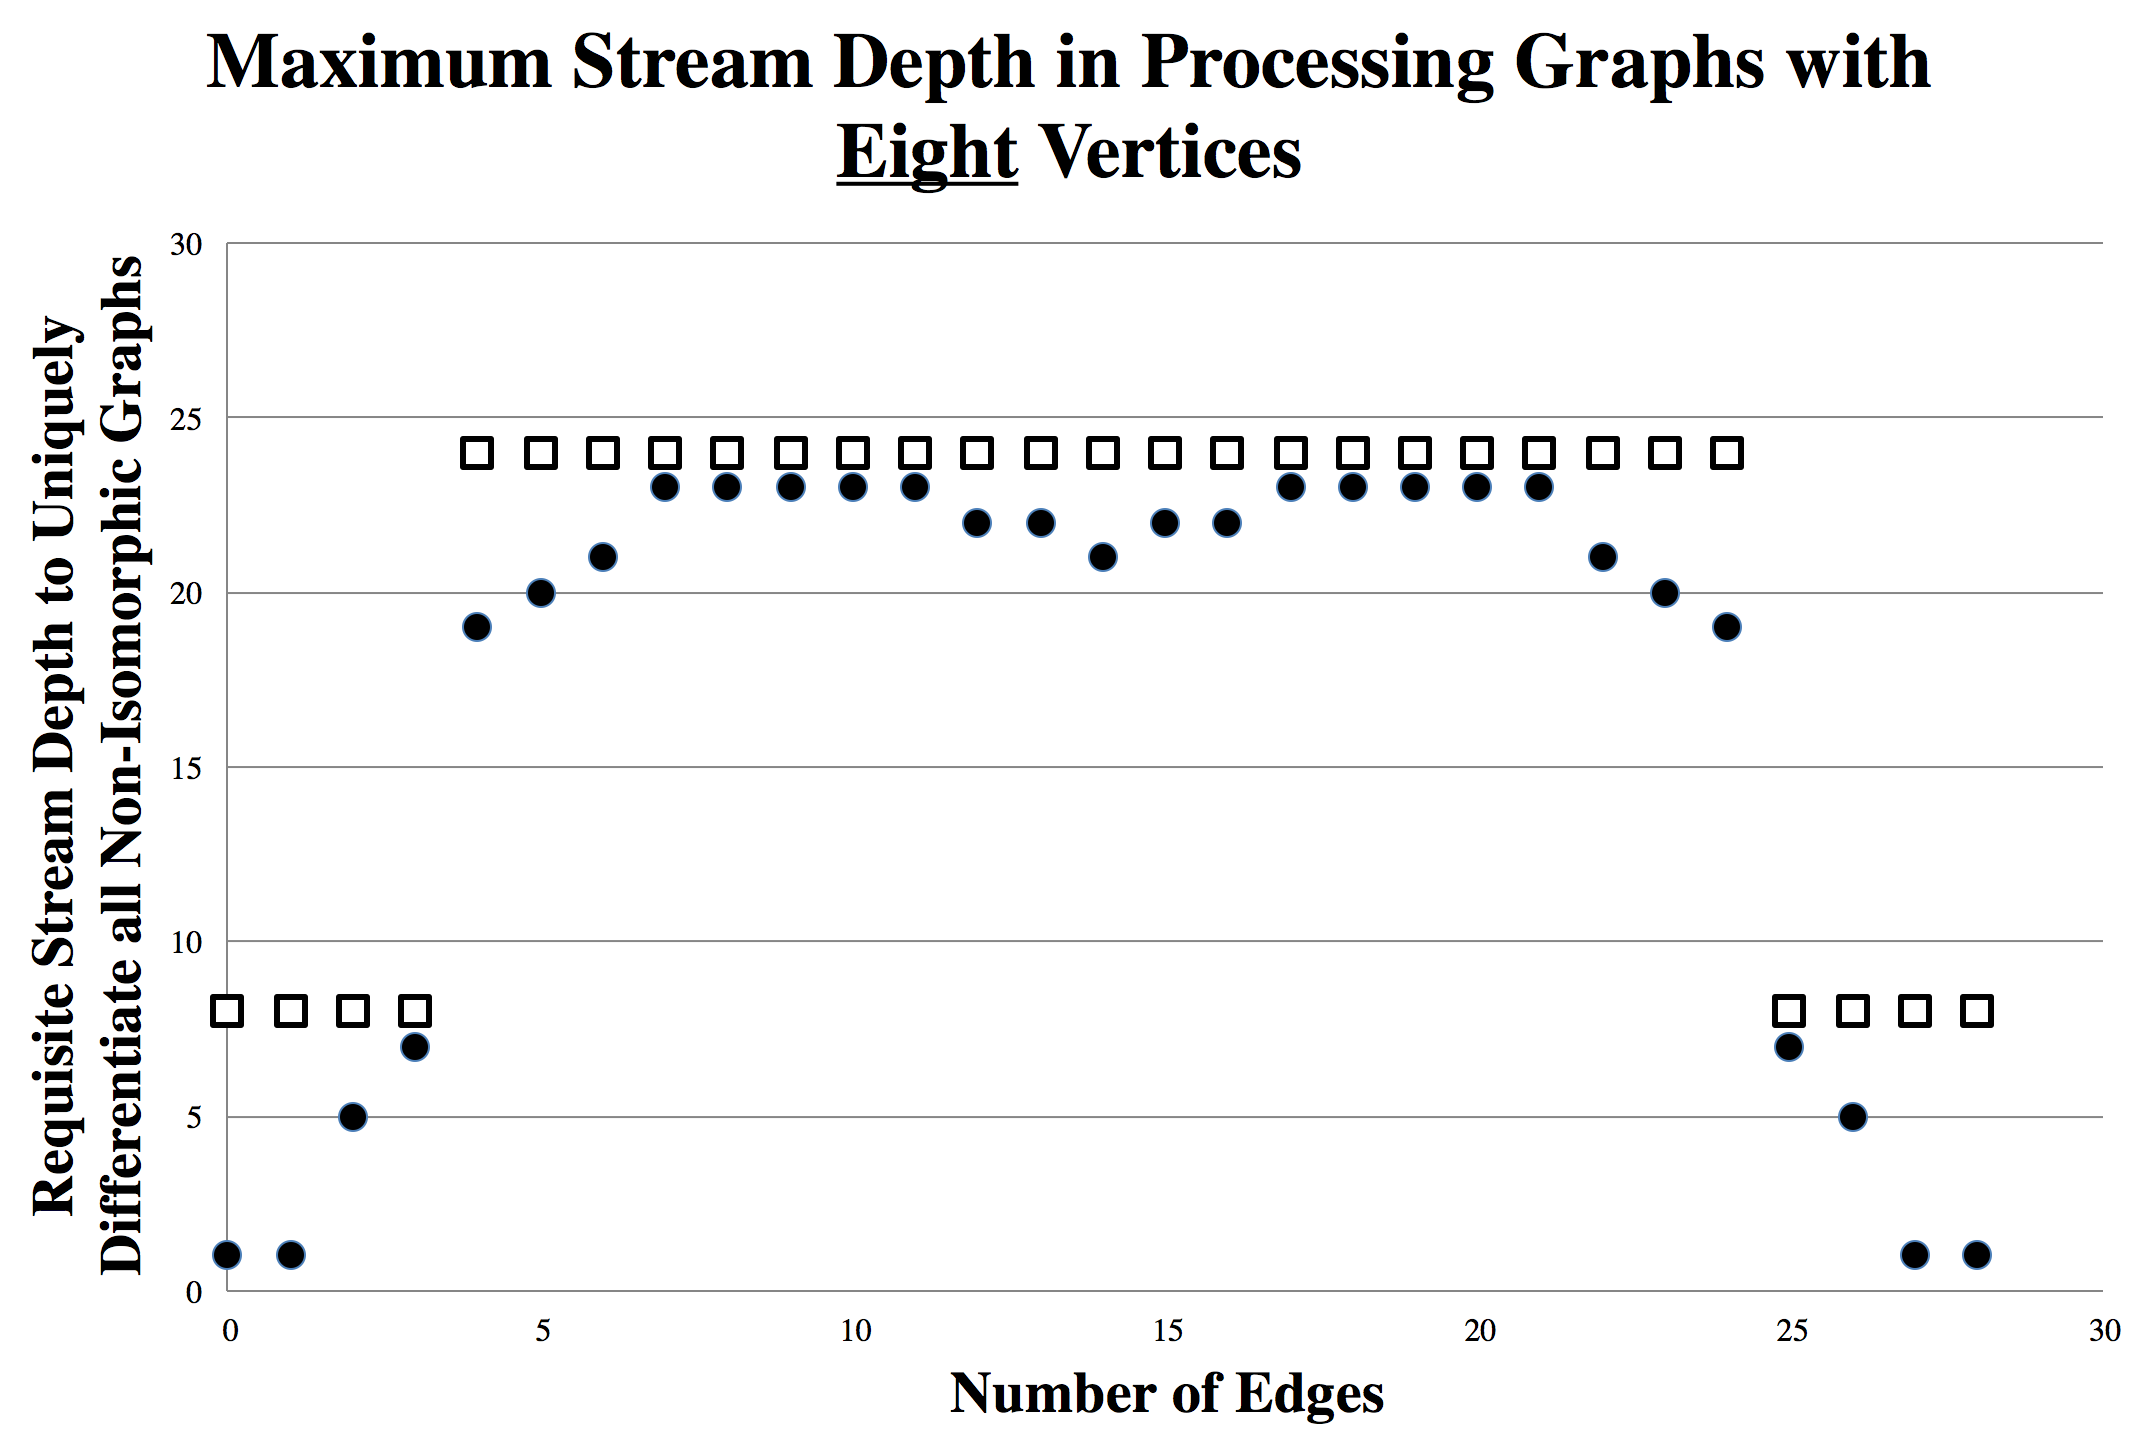
\includegraphics[width=\textwidth]{powercurve8}
\end{figure}

\begin{figure}[h]
\label{fig:powercurve9}
\caption{}
\centering
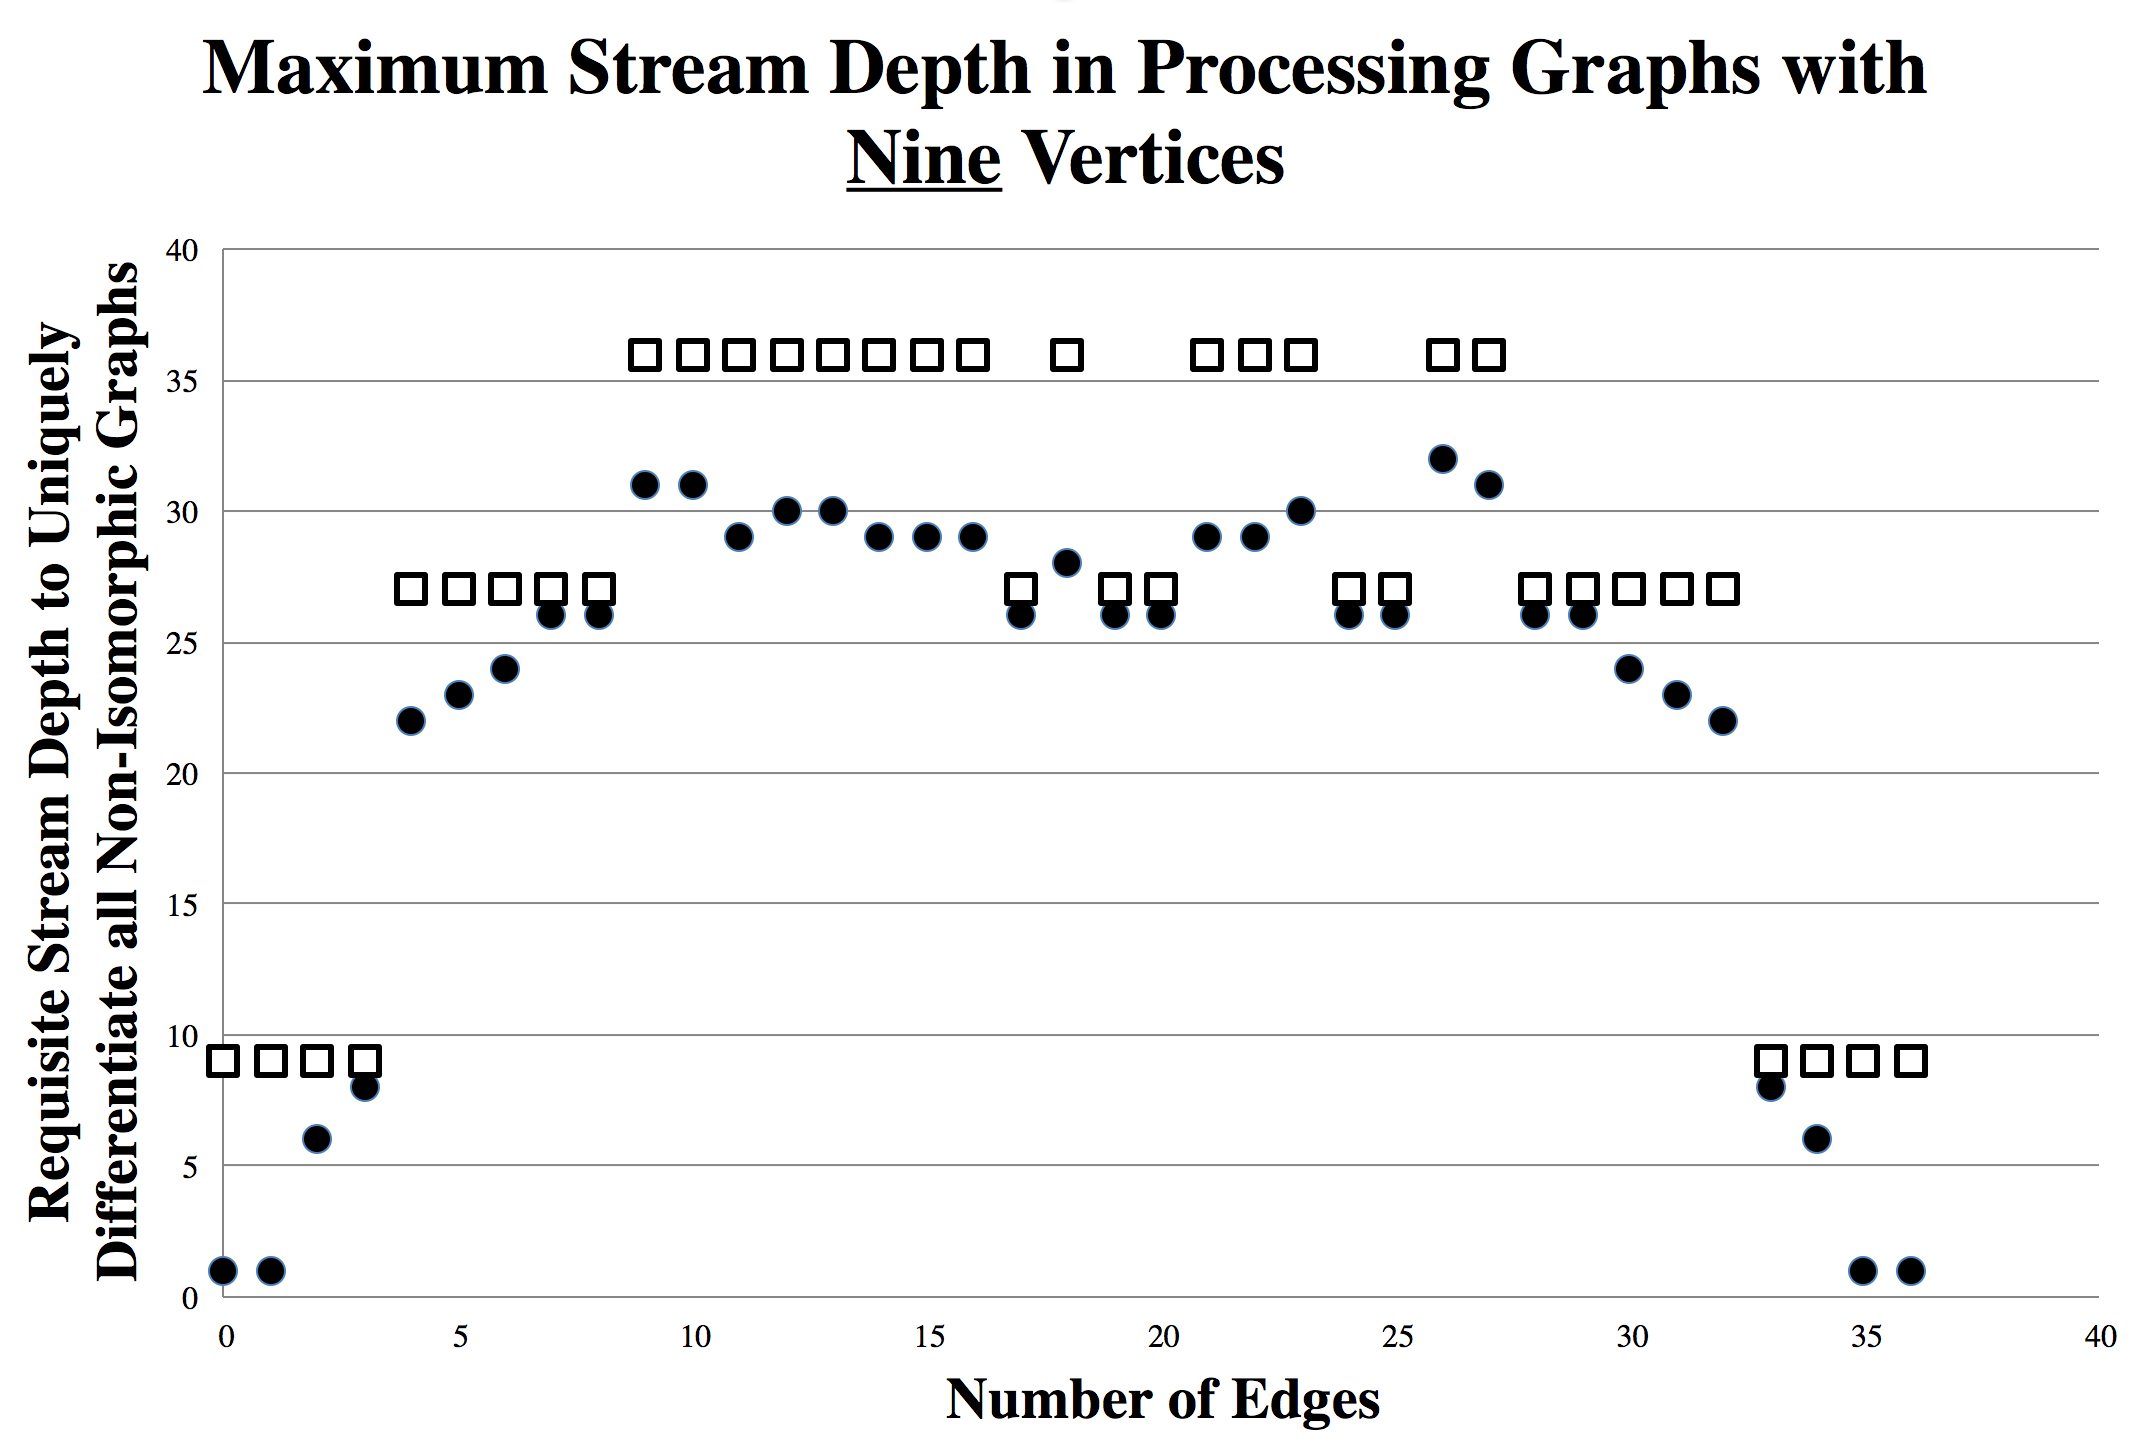
\includegraphics[width=\textwidth]{powercurve9}
\end{figure}

\begin{figure}[h]
\label{fig:powercurve10}
\caption{}
\centering
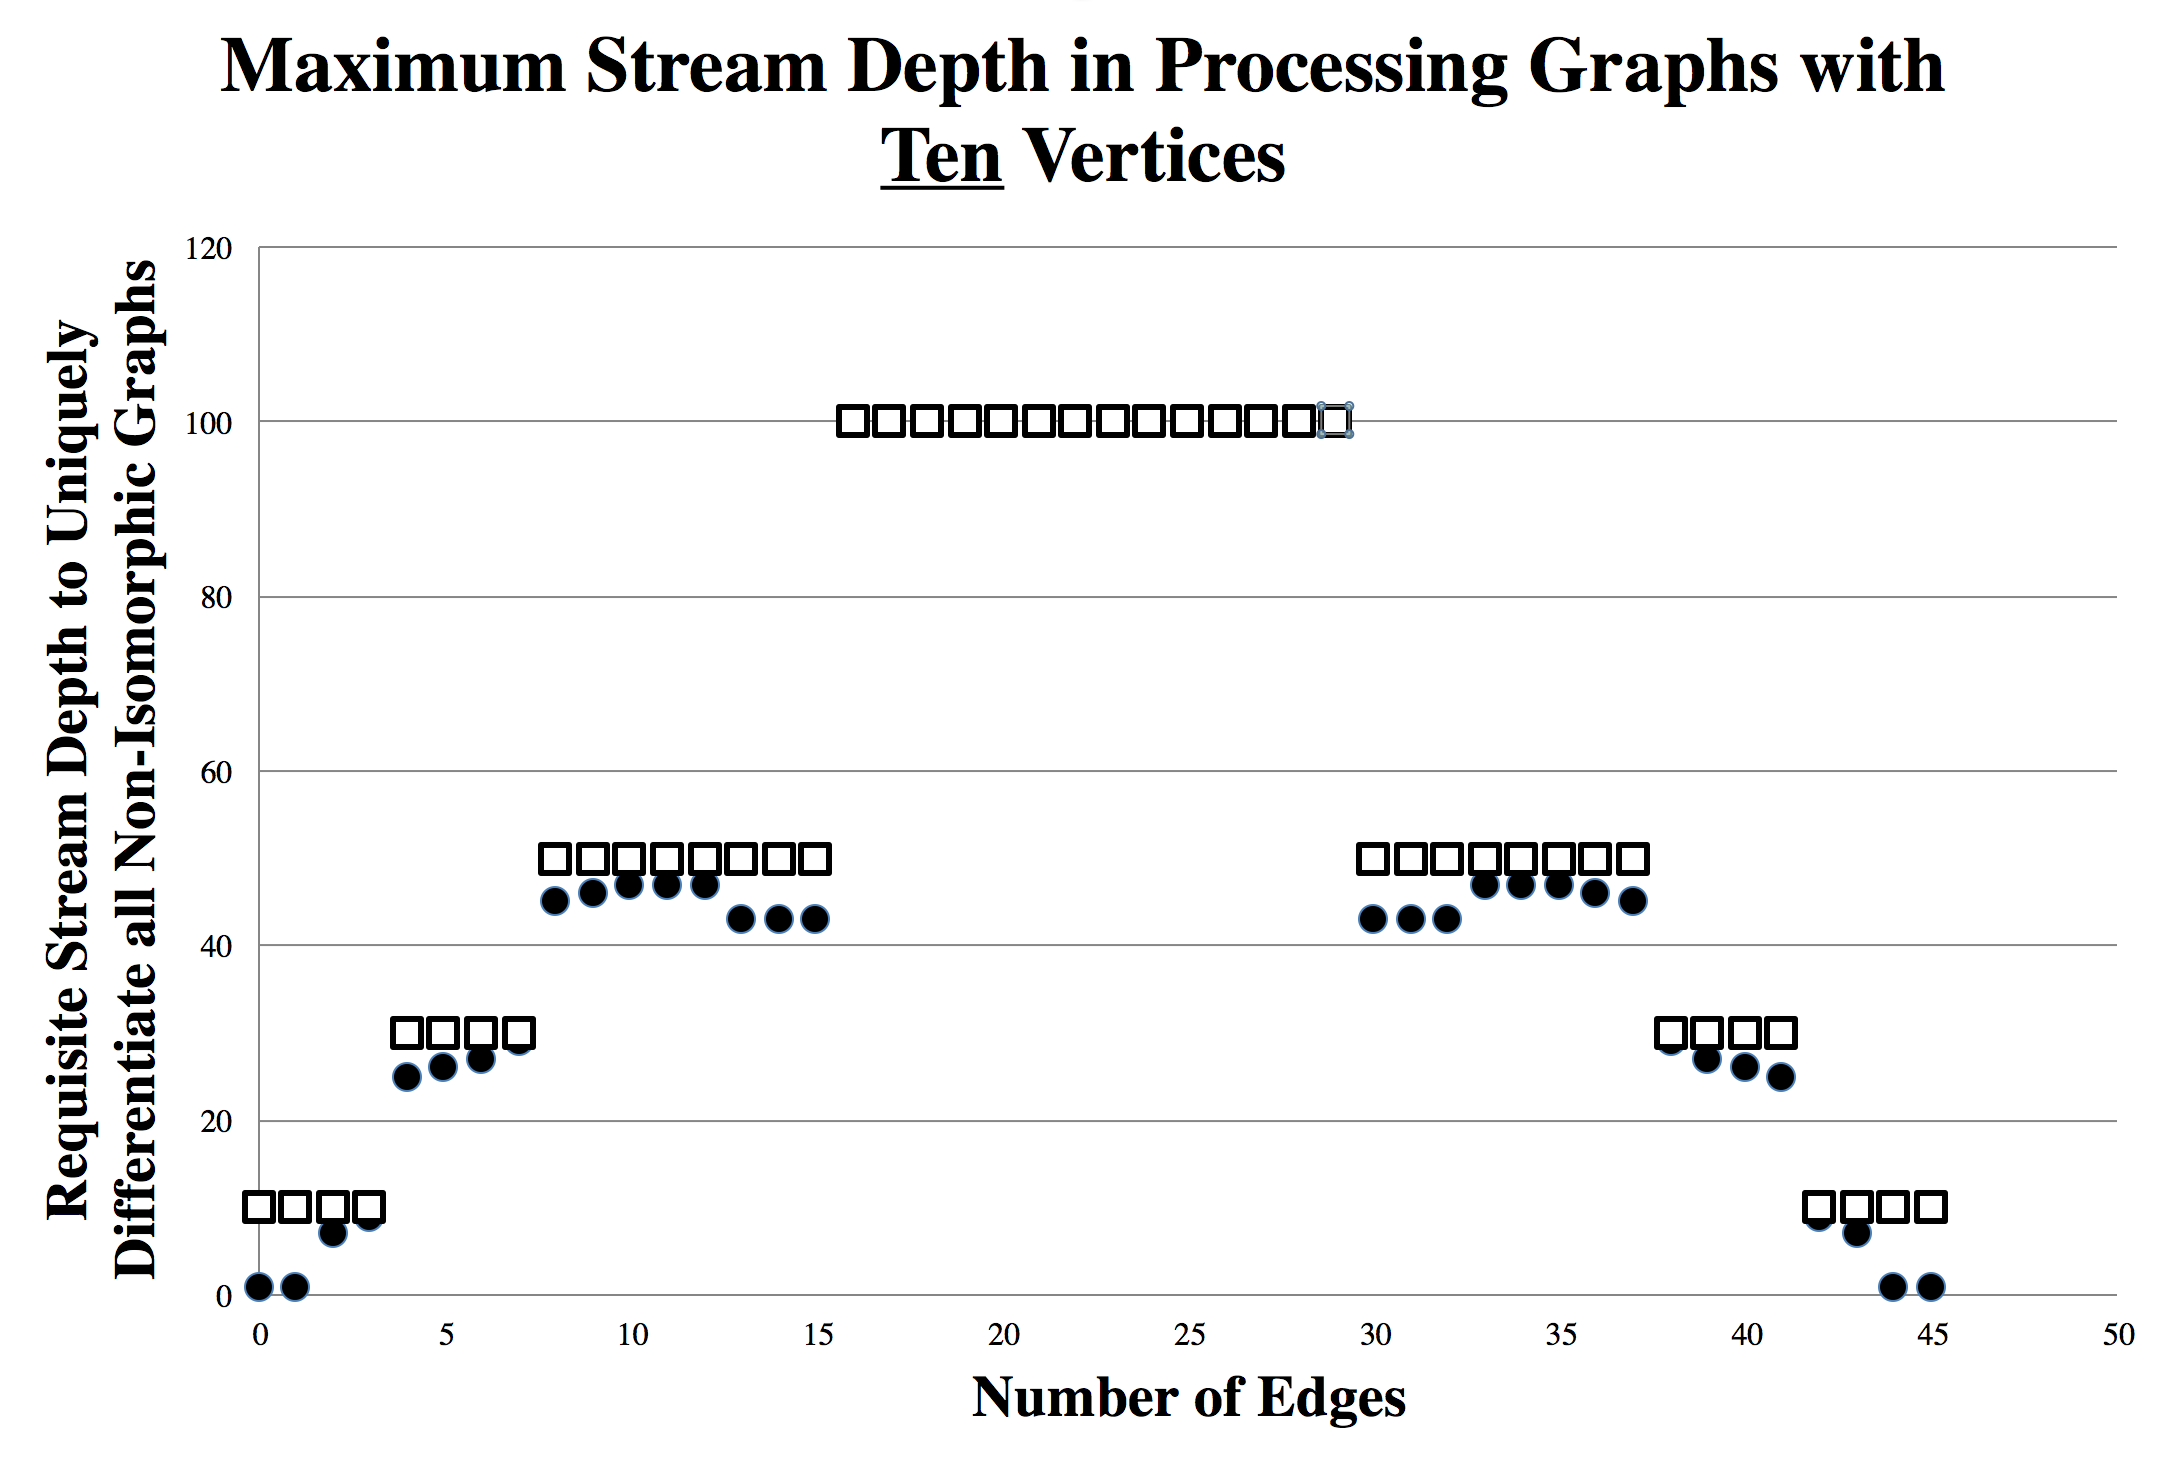
\includegraphics[width=\textwidth]{powercurve10}
\end{figure}

In each diagram, the dots represent the maximum trie depth, while the squares above them round that value up to the nearest `complete' depth.
By complete depth, we are referring to a depth divisible by the number of vertices within the graph.
This is relevant because these levels are the length of the cycles that correspond to all of the information gleaned from this length cycle and fewer.

\subsection{An Unexpected Dip}

What we see is counter to our expectations.
$P^*(S_{N, M})$ certainly is smaller at the fringes, but it actually dips in the middle, where the majority of the graphs are located.
Remember from chapter one that the number of graphs in each of these sets is maximized in the middle, while the ability to differentiate between them is actually maximized with connectivity around .25 and .75.

In figure \ref{powercurve10}, we see the same trend (slightly lower values for $N > 12$, than for $N \in (10, 12)$), despite the existence of co-cycles graphs, which push the middle up to 100 (maximal trie depth for N=10).

In figure \ref{powercurve9}, we see this trend exaggerated to the point that it distorts not only the granular values (the black dots), but the overall cycles length values (boxes).

It should be noted that the asymmetry in diagram \cite{powercurve9} was highly suspect to me.
I looked into it, and was able reproduce it using Matlab (in addition to the calculations in C).  
It turns out that the asymmetry is due to the lack of invertible equivalence in the Cycles invariant, and for some graphs in $S_{N=9, M=25}$ can be differentiated by their cycles values, while their inverses cannot.

This small set of experiments suggests an interesting property of graphs: it may be easier to differentiate between graphs which are half connected than a quarter connected, despite the fact that there are significantly more graphs which are half connected.


\chapter{Cycles as a Vertex Invariant}

A powerful feature of the cycles invariant is that it is not only discriminatory between graphs, it suggests potential isomorphisms between their vertices.
This section will discuss exactly how isomorphisms can be constructed and evaluated by using cycles as a vertex invariant.
Central to this chapter is the concept described earlier as Automorphism Equivalence Classes, or Similar Vertex Sets (SVS).

\section{Perfect Similar Vertex Sets}

A vertex-similar sets is a subset of the vertices of a graph such that for any pair of vertices in the set, there exists an automorphism which maps one to the other.
Note that vertex similarity is reflexive (as one-to-one mapping (such as an automorphism) is invertible). 
Also note that membership in vertex-similar sets is transitive (as we can simply use the `followed-by' operator on the component automorphism mappings).

Thus, all vertices in a graph can be partitioned into some number of similarity-sets, where every set has at least one element, and the union of the sets is the vertex set.
For the sake of simplicity, we will assume that there is some well-ordering over these sets, so that we are able to assign an order to each set within the collection of similar vertex sets.
In practice, this will be a practical function of how we go about computing the SVSes.

This construction is deeply tied to isomorphism checking and discovery.
If we have two graphs $G$ and $H$, and their Similar Vertex Sets are $SVS(G)$ and $SVS(H)$, based on the size of each set, we have a maximum number of potential isomorphisms.
First off, if we examine every $i$th paired set between $SVS(G)[i]$ and  $SVS(H)[i]$, if the sizes of the sets differ, then we can immediately reject the possibility of isomorphism between $G$ and $H$.
If the size of each component set are the same, we can check for isomorphism by brute force, by calculating every possible permutation between the paired sets, and then every combination of those permutations across all of the SVSes.
Though we can make many practical arguments which greatly simplify the number of these possibilities we have to test for isomorphism, it should be noted that in the overwhelming majority of cases, this simple algorithm only has to check \emph{one} mapping for an isomorphism.
This is by virtue of the fact the the overwhelming majority of graphs have only a single automorphism.

\section{Most Graphs Have One Automorphism}

This is by virtue of a simple fact: we can talk broadly about the average number of automorphisms in a set of graphs, and even better, we can calculate precise means for the average number of automorphisms for graphs of a certain size.
Remember that the number of undirected, non-looped, single-edge graphs (or as we have just been calling them, graphs), over N vertices has a known closed form.
We also know that the number of graph instances over N nodes is simply the number of undirected matrices over N nodes, $2^{E_{max}}$.
Finally, we know that the number of matrices 

$$ M_{reps}(g) = \frac{N!}{|Aut(g)|} $$
$$ \sum_{g \in G_{alg}} M_{reps}(g) = \sum_{g \in G_{alg}} \frac{N!}{|Aut(g)|} $$
$$ 2^{\frac{N^2 - N}{2}} = N! \sum_{g \in G_{alg}} \frac{1}{|Aut(g)|} $$
$$\frac{\sum_{g \in G_{alg}} \frac{1}{|Aut(g)|}}{|G_{alg}|} =  \frac{2^{\frac{N^2 - N}{2}}}{N! * |G_{alg}|} $$
$$ \xoverline{|Aut^{-1}(g)|} = \frac{2^{\frac{N^2 - N}{2}}}{N! * |G_{alg}|}$$

Though we don't have a closed form for this, a quick calculation pretty easy, and gives us a very clear trend.
In Figure \ref{fig:mostgraphsoneaut}, there are two figures shown.
The first plot shows the right hand side of the final equation, graphed for different values of N.
The second plot explores the difference between the first plot and one, and takes the logarithm to see how small the values get.

\begin{figure}[h]
\label{fig:mostgraphsoneaut}
\caption{\emph{Most Graphs Have Exactly One Automorphism} - It is clear that as N increases, the right hand side of our above equation approaches 1. Not only that, but it appears to do so exponentially fast.  The plot on the right shows a logarithmic linear approach to one.}
\centering
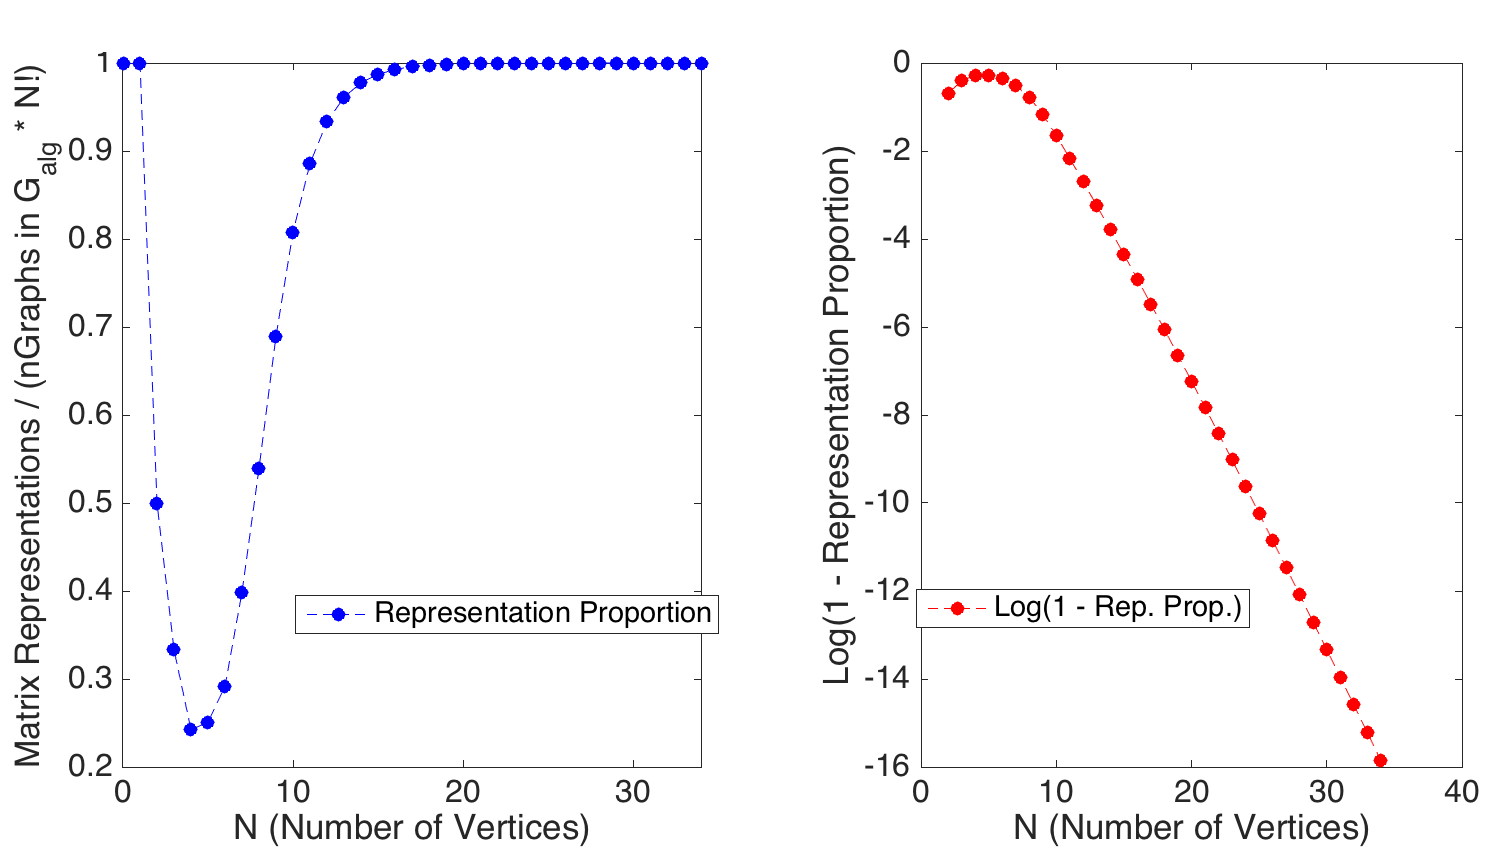
\includegraphics[width=\textwidth]{numGraphsAndMats}
\end{figure}

This should convince even a skeptical reader that for an average graph $g$ (even when treating it like an algebraic object), as $N$ increases, $\xoverline{|Aut(g)|} \rightarrow 1$.

\subsection{Implications for Perfectly Similar Vertex Sets}

Applying this back to our original purpose, we can reason that if a graph only has a single automorphism, then the only automorphism is the trivial automorphism.
Thus, the SVSes are a set of N distinct, one element sets, where each vertex is distinguishable from each other, and none share any automorphisms.
This makes checking for isomorphism between two random graphs trivial (if we have the SVSes), as the overwhelming majority of the time, we will only need to try the isomorphism implied by the direct, one to one mapping between the SVSes of the two graphs.

However, checking for Automorphisms between every single pair of vertices is clearly in a higher computational complexity class than testing for isomorphism.
Thus, we will use smart heuristics to develop quazi-similar vertex sets, which will enable us to get the benefits of SVSes (i.e. implying the isomorphisms to try) without actually proving that the automorphisms that define the SVSes exist.

\section{Quazi-Similar Vertex Sets}

Quazi-similar vertex sets are constructed with respect to a vertex invariant.
The vertex invariant is calculated for all vertices within the graph, and those with the same value are placed into the same set.
Transitivity and reflexivity clearly both hold under this definition.
Moreover, the ordering/comparability of vertex invariants gives us a natural way to order the sets within the QSVS.

In this section, we will describe how using the cycles invariant to generate QSVSes is highly successful at mirroring the true SVSes, and suggest an augmentation to cycles which correctly differentiates the two for all observed cases.



\section{Why $P^*<N$: Limitations on Cycles Usefulness}

\subsection{What is $P^*$, why does it matter?}

An ENORMOUS part of this thesis has thus far gone as assumed: what is $P$ (the maximum length cycle we are considering)?
When we are discussing cycles through a node, how long are the cycles we are considering?
The vertex invariant for cycles is clearly a vector, with the length of cycles corresponding to the place within the vector (cycles of length 2, 3, 4, etc.), but where do we draw the line?
To answer this question, I used a notion of `usefulness', to maximize the amount of information that we get out of the cycles invariant for the computation that we put into it.

Specifically, within the context of cycles as a vertex invariant, I started out with the assumption that all vertices share a single Similar Vertex Set (i.e. all are similar unless we have proof that they are not).
We then distinguish vertices by advancing P by one, we are in effect splitting this one class (or smaller classes) into smaller classes, based on the information gleaned by increasing the length of all invariant vectors by one.
This kinds of `breaking-down' leads us to a concrete notion of usefulness: for a given graph G, cycles is useful at a power $P_G$, where $P_G$ is the minimum value for P at which all of the vertex sets in the SVSes are as broken down as they can get (for any amount of P).
Thus, if we take the maximum of $P_G$ across all G, we will find a value $P^*$ at which point computation beyond this point is redundant.
This would enable us to more concretely talk about running time, and its tradeoffs.
What we find (through both computational exploration and theoretical justification) is that $P^*$ is contingent upon $N$, and specifically that:

\[ P^* = \begin{cases} 
      N-1 & \text{If N is odd} \\
      N-2 & \text{If N is even} \\
   \end{cases}
\]

\subsection{Observational Data: Diameter vs. $P_G$}

I first tried to explain $P_G$ as a function of the individual graph $G$.
Though this did not lead me anywhere directly, it did give me a clear idea of the upper bounds on $P_G$ for an individual graph.
Shown in figure \ref{fig:diamvsmaxpower} is a description of this relationship.  By no means is it rigid, but the coorelation is very strong.
It is also interesting (personally) just to see the diameter of a set of graphs laid out like this, just a side note.

\begin{figure}[h]
\label{fig:diamvsmaxpower}
\caption{\emph{Diameter Against $P_G$ with $N=9$} - The size and number next to each circle tell us how many graphs (as objects) fit into different sizes of diameter and $P_G$}
\centering
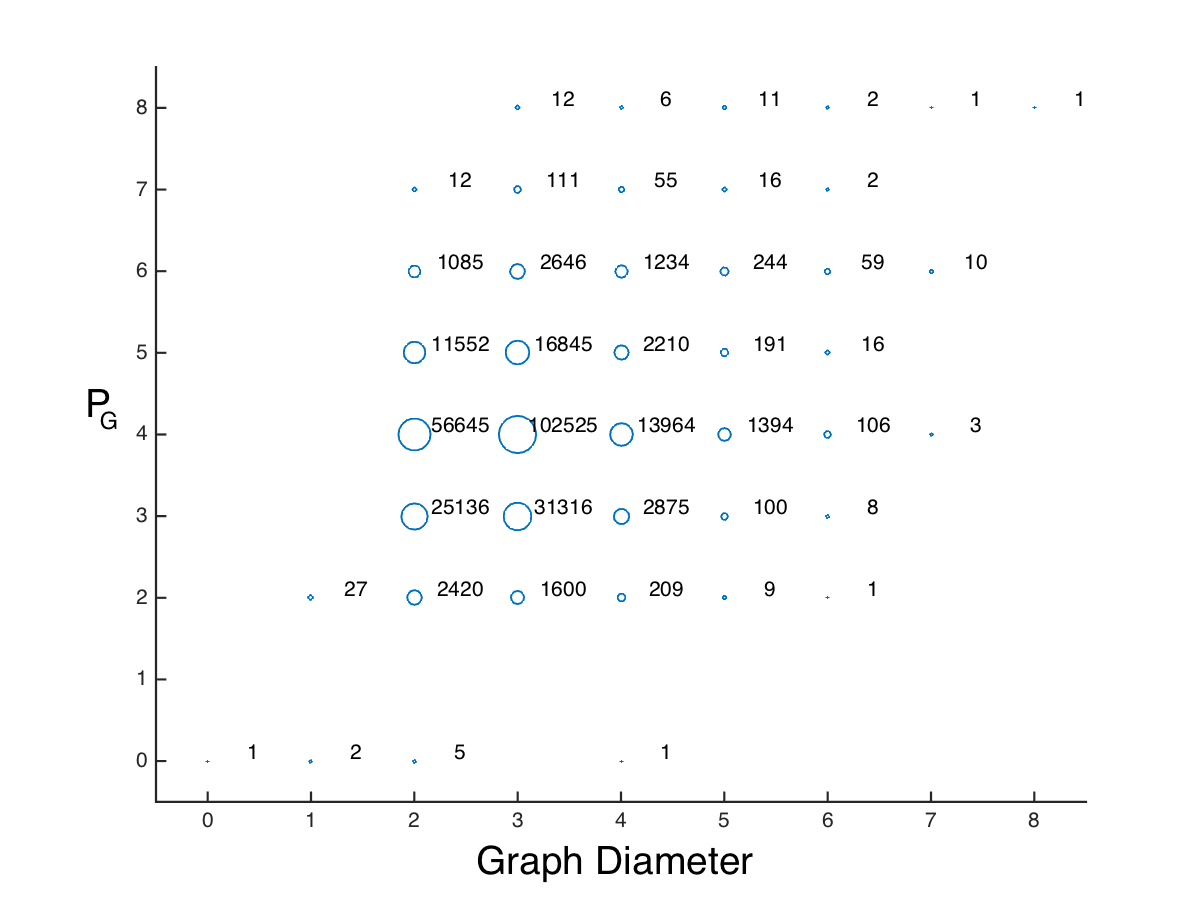
\includegraphics[width=\textwidth]{N9DiamVsDiffPower}
\end{figure}

Four things are consistent across all of the alike graphs (shown in an appendix):
\begin{itemize}
\item{There is consistently a maximum diameter for $P_G$, implying a $P^*$ for each as shown in the table below}
\item{There are never any graphs with $P_G = 1$, as we do not allow self loops }
\item{The Path graph ($P_N$), is always the lone member of the far upper right hand corner}
\item{The Cycle graph ($C_N$), always has $P_G$ equal to that of the Path graph}
\end{itemize}
The upper bound proposed by each one of the values for $P*(N)$ follows the pattern:
\[ P^* = \begin{cases} 
      N-1 & \text{If N is odd} \\
      N-2 & \text{If N is even} \\
   \end{cases}
\]
for $N <=9$. This sets up a strong case for this as a target hypothesis, but we still must prove it.

\subsection{Theoretical Justification: $P_N$ versus $C_N$}
Why does the proposed value for $P^*$ make sense?

This proof consists of two parts, the first is why $P_{P_N} = \text{the proposed} P^*$ for the Path graph ($P_N$), the second describes why all other graphs $G$ have $P_G \leq P_{P_N}$.

Part 1: \emph{Distinguishing between vertices in the path graph requires $P_{P_N} = N - 1 - ((N+1)\%2)$.}

Start all vertices in the same assumed similarity set, and assume that $P = 0$.
When we increase $P$ to 2, all vertices have degree 2 (the second entry in the cycles invariant) except for the two terminuses, thus the two terminuses are split off from the original quazi-similarity set, as they have been distinguished at $P=2$ by their cycles invariant.
When we increase $P$ to 4, the two nodes adjacent to the two terminuses are now distinguished (as they are now `missing' a path of length four that they would have had if they were further in toward the center of the path graph). 
There are now $N-4$ vertices remaining in the original quazi-similar vertex set.
From this, it is clear to see that for an arbitrarily large path graph, for $P=2K$, there will be $N-2K$ elements in the original QSVS.
We will have \emph{fully distinguished} all of the vertices into distinct QSVSes which are true to the SVSes when the original QSVS contains only the `middle' node(s).

In the even case $N = 2K, K \in Z$, this occurs when we have 
$$P = 2\ceil{\frac{N-2}{2}} = 2\ceil{\frac{2K}{2} - 1} = 2\ceil{K - 1} = 2(K - 1) = 2K - 2 = N - 2$$
In the odd case $N = 2K +1, K \in Z$, this occurs when we have 
$$P = 2\ceil{\frac{N-2}{2}}  = 2\ceil{\frac{2K+1- 2}{2}} = 2\ceil{K - 1/2} = 2K = N - 1 $$

Thus, we know that 
\[ P_{P_N} = \begin{cases} 
      N-1 & \text{If N is odd} \\
      N-2 & \text{If N is even} \\
   \end{cases}
\]

\section{Improving upon QSVS with Flagged Cycles}

The quality of the QSVS is generally described as how close they are to the true SVSes.
In other words, quality is a measure of how frequently does a QSVS contain two or more subsets that should be independent SVSes.
Though Cycles as a vertex invariant produces QSVSes which mirror SVSes with high probability, we should examine the failures cases to see if we can do better.

We will accomplish this via a methodology I am calling `flagging' after I have seen that a few times in the literature.
Flagging (or Marking) is the process of taking a graph and appending a single vertex to it which is connected by a single edge to some target vertex in the graph.
Flagging frequently modifies graph structure enough to see impacts with solid results.

For example, if we have two co-spectral graphs, and we are curious whether or not an isomorphism exists between the two of them, we can append a flag on each one of the vertices which must be mapped together in a potential isomorphism, and then take the chromatic polynomial again.
If the new (flagged) graphs differ in their chromatic polynomial, then the two vertices that were flagged cannot have an isomorphism to one another, as modifying two isomorphic graphs in a deterministic way should preserve isomorphism.
We use this principle in the pursuit of fully differentiating a set of QSVS into a refined state that more clearly mirrors SVSes.

\subsection{Appending a Flag, Somewhat Predictable}

Our methodology for modifying the QSVSes is simple: first, calculate the QSVSes using the Cycles invariant.
For each of the sets within the QSVSes with more than one element, perform a flagging operation K times, if the set has K elements, which results in K different graphs.
Calculate the cycles graph invariant over each of these graphs.
If the cycles invariants for any two of the K graphs differs, then split apart the set of vertices into two (or more) new QSVSes, one for each different value of the graph invariant associated with the graph formed by flagging each vertex.
What a mouth-full!

An interesting piece of this is that we can actually predict some of the values that the newly created, flagged graphs, will have for their cycles invariant values.
Specifically, we can predict the number of cycles for the flag vertex, as each one of the cycles that it is a part of must go to and from the flagged vertex, and we already knew how many of those there were from the original cycles function.
Additionally, we can predict the change in the number of cycles for the flagged vertex, as we knew its cycle profile before, and the addition of a single vertex on to it can be interpreted as a recursive definition, where cycles are broken into components that travel back (and forth) from the flag vertex and those that exist within the graph.
Though difficult to explain via formulae and words, I would encourage a skeptical reader to check out my code at (/Thesis/Matlab/constituentpaths/predictPathsOfAddingOneVertex.m).

Equally interesting (to the fact that we \emph{can} predict paths for these two nodes when just given the cycles invariant) is that we \emph{cannot} make any further predictions about the flagged cycles values based solely on the plain cycles values.
We know this to be true because in co-cycles graphs, we frequently get different flagged cycles graph invariants when we flag vertices which are suggested to be isomorphic (but are not).
This is a good piece of information to know because it gives us proof that flagging is not some kind of manipulation of information that we already have, it represents a way to get pieces of information that are tangibly new.

\subsection{Intuitive Justification for Flagging}

This section is not grounded in proof, but gives a conceptual reason that flagging works at further discriminating between vertices that we think might be automorphic.
Cycles is really a rough description of the `neighborhood' of a vertex within its context in the graph.
Cycles tells us about the way that energy reverberates around a structure.
One conceptual tool I like is to think about electricity flowing (bidirectionally) around a circuit, and measuring the self-connectivity or resistance.

Flagging a node changes that dynamic.
It changes it in a way that we understand and can predict for the flagged vertex and the flag vertex.
However, it also changes the way that cycles `reverberate' through the flagged vertex, and in doing so, changes the cycles invariant at other vertices.
We can even think of this in more concrete terms: take the cycles invariant for the flagged graph (without sorting), then subtract off the cycles invariant for the non-flagged graph (again, without sorting).

This tells you exactly how many new cycles have been created which pass through the flagged node at least once.
We call this modified matrix the \emph{excess cycles} matrix.
Note that this is \emph{not} the same as the row for the flagged cycles matrix, and actually encodes significantly more information (the constituents of those paths, not only that they exist).
In doing so, we actually get tangible information about the connectivity of each of the nodes.
From the excess cycles matrix, we can calculate the distance between the flagged vertex and each of the other vertices in the graph.
We can calculate the relative makeup of each of the added cycles (how many pass through each vertex, and how many times does each double back on itself), among a large number of other features.

The intuitive justification for flagging is compelling, and if I had another month to puzzle away at this problem, this is probably the area I would spend the most time focusing on.

\subsection{Analytical Support for Flagging, and an Open Question}

The analytical support for flagging is strong:
for all graphs of size $N<=10$, cycles with flagging as a mechanism for QSVS generation correctly generated QSVSes which turned out to be the same as the SVSes.
No counterexamples were found where cycles with flagging fails to be anything short of a perfect vertex invariant.

This begs an open question: is it possible that cycles with flagging is complete as a vertex invariant?
Is it possible that this metric fully determines the automorphism sets of vertices? Maybe.
However, it is more likely (based on the raw number of graphs out there) that we have only kicked the proverbial can further down the road.
For one, the raw amount of information required in Cycles with flagging is N times the amount of information required for cycles comparison.
This alone should tell us to expect a higher threshold for failure.

That being said, there are properties that are reconstructable from excess cycles computations that make me think that flagging might have some higher order justification.
I would love to spend another few months thinking of equations that I can use to reconstruct $A$ (or better yet, determine $A$) from flagged cycles.

%\section{Limitations to Augmentation}
%\subsection{A Second Augmentation Hypothesis}

\chapter{Canonical Labeling Using Cycles}


\section{Background}
A canonical labeling of a graph is a labeling of edges in a way that is consistent across all isomorphic graph instances of the same graph.
Given two graphs and their canonical labelings, graph isomorphism is then a simple quadratic-time check to make sure that alike-labeled vertices preserve all adjacencies and non-adjacencies. 
Thus, any canonical labeling algorithm is in $GI$, the time complexity class of the graph isomorphism problem.

Many parts of my coding projects required the use of a canonical labeler.
Sometimes this was because I wanted to check for isomorphisms on a broad set of graphs, a problem that is possible to complete quickly given the lexicographical nature of canonical labels.
Though there exist good algorithms for determining canonical labeling, I wanted to create my own, both as an exercise in implementation, and in algorithm design.
The result of this process is an algorithm which is relatively slow, but whose time growth is small relative to faster algorithms.

\section{Augmented Paths}

\section{A Consistent Algorithm}
The algorithm has a simple interpretation. 
It divides all of the vertices of the graphs into disjoint (covering) sets based on the value of the cycles vertex invariant.
For each of these sets with more than one vertex, a second round of `augmented paths' is performed to further divide sets, if possible.
It sorts each of these classes by its size, then by its paths values.
Each of these sorts is performed in a consistent way, which is irrespective of the original labeling of the graph.

Once the order of the sets is sorted, we consider every possible permutation of the values within each of the sets so that every possible ordering of vertexes is possible, with the constraint that each set element remains in the higher level order established by the sets themselves.
We traverse through these permutations and select the matrix which is lexicographically the `smallest'.
A clever optimization allows us to not generate any permutations which are automatically `larger' than the thus far `smallest' matrix.

I wrote and optimized the algorithm for Matlab (as that is the slowest of my use cases), but then worked on implementing it in C and Javascript.
All three versions of this code are available in my online repository documenting my thesis work.
The Matlab code provides detailed explanations of each piece of the code, why I implemented it that way, and the thoughts that went into it.

\section{Time Growth Comparisons to Faster Algorithms}
Any discussion of a homegrown algorithm would be either incomplete or intentionally salacious without a discussion of how it compares to out of the box algorithms.
For these benchmarks, I established two datasets, one of 10000 randomly generated graphs of size ten to fifty using an Erdos-Renyi model, and one using a graph model which is more likely to produce highly automorphic graphs (discussed in detail in chapter 6).
For both of these models we used a probability of $p=0.5$, as these are typically the graphs that are hardest to discriminate against.

To give perspective to my own time results, I used an established and well optimized piece of code, the canonical labeler from the NAUTY package.
A summary of the results is shown below, alongside equations which estimate their overall running time with the above parameters.
From these figures it is clear that the NAUTY package outperforms my canonical labeler, but that my labeler appears to have a lower growth rate.
I would imagine that this difference can be attributed to the large lengths my labeler goes to to minimize the number of permutations that are checked.
NAUTY's algorithm uses simpler heuristics (such as X and X) to eliminate permutations, while mine uses significantly more power to make likely better informed choices.


\chapter{Random Graph Generators and Automorphisms}

\section{Random Graph Models}

The field of random graph theory was started with two independent papers in 1959, each defining models for generating and analyzing random graphs.
A \emph{random graph model} is any system of generating graphs with the influence of chance, with various constraints that describe the desired properties of the resulting graphs.
These two papers began a trend in graph theory that allowed theoreticians and algorithm designers to think about efficiency differently, particularly on NP-Hard and NP-Complete graph algorithms.
Rather than concerning themselves with worst case run time, theoreticians began describing and designing algorithms to satisfy ideas of average case running time over the `class of random graphs'.
Random graphs served as a new lens through which theory could pivot away from the worst case, instead handling common and general cases of problems that were either proven to be impossible in the worst case, or suspected to be so. 

A few examples from the years following showed that random graph theory lent a new life to the challenging problems of CITE, CITE and CITE.
In this chapter, we will discuss multiple models of random graph generation, examine the strengths and flaws of each, and propose alternative mechanisms by which graphs can be generated for more theoretical applications and algorithms.

It is important to recognize that there has been an increase in interest in alternative random graph models in the last ten years.
The majority of these papers focus on exponential random graph models, which are centered around the study of network structure with local and global patterns of connection.
For example, the internet (if sites are viewed as vertices and links as edges), has an exponential in-degree distribution (many more people link to cnn.com than gradybward.com) \cite{exponentialgraphs}.
Another set of random graph models tries to model social networks, which are categorized by cliques (groups of friends), with alternative connections that symbolize non-group friendships.
For either of these models, algorithmic theory is inadequate if it treats all graphs as equally likely, or if it treats all graph instances as equally likely.
Though this section is not focused on these models, it does adapt some of the characteristics and heuristics of this pursuit to a different goal, of establishing a random graph model for testing algorithms over the set of all graphs.

In this pursuit, we will question what we mean when we say `random' graphs, and make explicit the assumptions, aims and valid applications of any one of our models. 

\subsection{The Erd\"os-R\'enyi Model(s)}

In their seminal paper on random graph theory, Paul Erd\"os and Alfred R\'enyi proposed two different models for random graph generation.
The first of these models will be outlined in this section, and will be referred to as the Erd\"os-R\'enyi Model.
The second was laid out in the same 1959 paper, but was also discovered by an independent contemporaneous mathematician, Edgar Gilbert.
For the sake of clarity, we will refer to the contemporaneously described model as the Gilbert Model, and the one that is about to be outlined as the Erd\"os-R\'enyi Model.

The model $G(N, M$) is defined as choosing a graph G with uniform probability from the set of all graph instances with $N$ edges and $M$ vertices.
The size of this set is $\binom{E_{max}}{M}$, where $E_{max} = \frac{1}{2}(N^2 - N)$ represents the maximum number of vertices possible in a graph over $N$ vertices.
Though the probability of getting any graph \emph{instance} with $N$ and $M$ edges out of this model is uniform, the probability of getting any graph with those constraints is not.
Since the number of representations of a graph fluctuates along with other properties of the graph, this random generator has the flaw that certain graphs are more heavily weighted than others.
This is a flaw that we will discuss at length in discussion of the Gilbert Model.

In the study of random graphs, the Erd\"os-R\'enyi model has not been as popular as the Gilbert model because it is more cumbersome to deal with, and has fewer concrete applications CITE.
Though some papers have utilized this model (namely CITE and CITE), the majority of theory is better suited to the combinatorial and probabilistic methods that are made useful by the Gilbert model.
Though knowing the number of edges in a graph gives us some information about the graph, it turns out that the probability of a given edge, and the guarantee of its independence, is significantly more malleable to theoretic goals.

\subsection{The Gilbert Model}

The second model, which we will call the Gilbert model, comes from the mathematician Edgar Gilbert (as well as Erd\"os and R\'enyi) and is denoted $G(n, p)$.
In the Gilbert model, $n$ specifies $N$, the number of vertices in the graph, and every pair of vertices is connected by an edge with a fixed and independent probability $p$.
The Gilbert model is both intuitively pleasing, justified by real world use, and has convenient properties for proof.

The Gilbert Model is an effective model for real world applications where graphs are thought of as occurring naturally without oversight or intervention.
If we think about the configuration of the a network generated by actors acting randomly, the Gilbert model is appropriate.
For example, consider a cocktail party among strangers, where the odds that any two people have a conversation in a given evening are likely independent and uniform.
Or, consider the reproduction of coral, where fertilization of one coral by another is reasonably random through the fluid dynamics that carry, combine and disseminate their pollen.
Gilbert's model gives us the language to describe graphs that pop up in wide-ranging uses, and a model to express the assumptions we frequently make about graphs in practical applications.

Additionally, the Gilbert Model allows us to make bold proof-based claims about random graphs through established combinatorial and probabilistic methods.
For example, if we try to estimate the number of edges within the a Gilbert graph, we simply are asking the binomial question with $n$ and $p$, and we have a readily available probability distribution to answer our questions.
A more interesting example arises when we ask about the number of triangles expected in a large graph.
If our graph is sufficiently large enough, the existence of one triangle does not impact the potential existence of another.
We can express the number of triangles as a simple combinatorial problem: multiply the total number of triangles possible $\binom{N}{3}$ by the probability of all three edges existing $(p^3)$.
This shows how combinatorics gives us tools to deal with Gilbert random graphs, and to make theoretical statements about expectations of the properties of these graphs.

Finally, the Gilbert model has a revelatory connection to matrix representation.
Consider the model with a fixed probability of $p=0.5$ and some fixed $N$.
We will show that this random generator has a uniform probability of selecting any matrix from the set of all valid graph instances of size $N$.

Consider the range of integers $[0, K^2 - 1]$.
If we assume numbers are left-padded with infinite zeros, the $b$th bit of a randomly selected integer from this range has an equal probability of being a 1 or a 0, as exactly half of these numbers have each bit set.
This is trivially true through the fact that there are $K^2$ integers in this range, and $K^2$ different bit strings.
Since each bit string is only achievable with exact probability $(0.5)^K$, each integer is generated with the same, uniform probability.
We will reshape the bit-string into representing each one of the edge variables, and we let $K = E_{max} = \frac{1}{2}(V^2 - V)$.
This establishes a connection between the Gilbert model and a randomly selected matrix from the set of matrices which represent our definition of valid graphs. 
This connection is intuitively pleasing, but further investigation should also show that its implies skewed results for some algorithms which rely on it.

\subsection{Isomorphism Under the Gilbert Model}

One of the first places that theoreticians turned their attention toward after the start of the study of random graphs was the problem of Graph Isomorphism.
The dominant lens of that study was the discussion of naming a class of graphs, and having the following proof structure:
\begin{itemize}
\item{The class of graphs is closed under isomorphism (i.e. all graph instances are in the class of graphs)}
\item{The class of graphs includes a large proportion of all graph \emph{instances}}
\item{Any two graph instances in the class of graphs can be determined isomorphic or not in polynomial time}
\end{itemize}
This approach was undertaken by a large number of theoreticians in the 1960s and 1970s.
A secondary component of these papers became the discussion of alternative algorithms which could solve the cases that were not solved for by the large model of the paper.
It seemed (to paraphrase from Erdos), that graph theoreticians were going to chip away at the problem of graph isomorphism until there was nothing left to chip away.
Yet, as it went forward, the increasingly restricted set of graphs for which no fast algorithm was known did not vanish.
Instead, theoreticians (pardon the projection) were surprised to find that Graph Isomorphism was a hydra that they couldn't vanquish through these means.
No matter the number of large classes of graphs they covered, no matter the diminishing proportion of graphs that were left uncovered, they couldn't find a way to solve all cases.

Hindsight is clear, and we can see that the theoreticians' realization was really a self-reflexive commentary on the work that we are going to be doing in this section.
What they had discovered is that the easy cases in isomorphism are exponentially (in fact, factorially) more common under a Gilbert model than they are if we treat them as algebraic objects.
Thus, even as they shrunk the probability of seeing one of these highly automorphic graphs under a gilbert model, they did little to increase the overall number of graphs that their algorithms covered.

The work we are going to do in this report is taking the opposite approach.
Rather than trying to create algorithms that only cover a set of easy to handle graphs, we are going to ask how we can explicitly look for the harder cases.
There are a number of justifications for this kind of work, but one simple one is the evaluation and clarification of random graph models.
Initial attempts at modeling social networks, first through gilbert models, then through exponential models, failed to appropriately assess the true nature of the problem.
Similarly, algorithm designers who use a gilbert model to test against the `average' graph should have their algorithms checked against a truly `average' graph.

Treating graph instances as graphs allows theoreticians to use easier math, and allows algorithm designers to inflate their claims.
In the next section, we will show how a simple problem (like graph isomorphism) has dramatically different theoretical and experimental analysis when performed over all graphs than when it is performed over all graph instances.

%----------------------------------------------------------------------------------

\section{Disconnect from Graphs as Algebraic Objects}

Though it is the foundation for most probabilistic random graph theory, the Gilbert model is has a different meaning than we typically think when discussing `random' generators of other kinds.
When we consider most other discussions of `uniform randomness', we state the assumption that the result element was selected from its set with a uniform probability.
Moreover, we generally assume that each object within that pool was represented the same number of times.
When I say `a randomly generated integer from the range', we are all agreeing on assumptions of what integers fall within this range, as well as how many times each is in our pool for selection (namely, once). 
Whereas, when I say `a randomly selected word from a book', there is the possibility that common words are more likely to occur, or it could mean that I found the unique set of words in the book, and I am selecting from that.

This is where random graph theory and colloquial understandings of randomness miss one another.
Throughout this work I have gone to great lengths to distinguish between graphs (an entity that has a given structure), and graph instances (a given representation of that structure).
Most graphs have many distinct graph instances; many different ways of representing themselves, but this number varies as a function of the properties of the graph.

The problem with the two models outlined above is that they select a random \emph{graph instance} with a uniform probability, but this does not translate to our understanding of graphs as algebraic objects, which denote structure irrespective of representation.
Thus, a model which chooses graph instances with uniform probability does not choose graphs with uniform probability, just as selecting a word at random off of the page of a book is not equivalent to selecting a word from all of the words in the book with uniform probability.

Consider an illustrative example with two graphs, G and H, on N vertices and M edges.
Graph G has only the trivial automorphism, and Graph H has an automorphism group with 20 elements.
It was shown by XXX in CITE that the number of distinct matrix representations (and thus distinct labelings) of a graph is equal to $\frac{N!}{|Aut(G)|}$.
Thus, the number of graph instances that represent graph G is $N!$, while the number of graph instances that represent graph H is $\frac{N!}{20}$.
Since graph instances are really just a way about talking about the number of matrices which represent the graph, this means that in the set of all valid undirected, non-looped graph matrices, there are 20 times as many which represent G as represent H.
This is critical because the two models of selecting random graphs select a matrix with a certain number of ones (some number of edges) with equal probability.
Even when the probability is not $p=0.5$ as it was in the illustrated case, it is clear that this is true.
This means that the probability of selecting a matrix which represents graph G is twenty times more likely than selecting a matrix which represents graph H under either `random' graph generator.

Though this seems like a semantic difference, as I will show over the next several sections, it has critical implications for the algorithms that use it to argue about computational complexity.

\subsection{Comparing the Distribution of Graph Connectivity}

In Chapter 1, we described the overall distribution of graphs as algebraic objects with respect to their connectivity.
We can also model the connectivity if we are considering the set of graph instances.
Since there is a one to one correspondence between graph instances and the set of all valid zero-diagonaled, binary symmetric matrices, we can discuss the connectivity of graph instances as a function of the binomial distribution.
That is because we can view the process of random graph instance generation under the gilbert model with probability .5 as a sequence of disjoint (as equally probable) binary variables, one per edge.
Thus the number of edges in a Gilbert random graph follows a binomial distribution with $E_{max}$ trials and fixed probability of success $\frac{1}{2}$.

The variance of such a model is known to be 
$$Var(Binom(n, p)) = (1-p) * p * n = E_{max} * .5 * .5 = \frac{E_{max}}{4}$$
Since we want to normalize our distribution so that the x values represent connectivity, we divide by the number of edges possible (after we convert to the standard deviation by taking the square root:
$$\sigma_{norm}(|E(G_{inst})|) = \frac{\sqrt{Var(Binom(E_{max}, .5))}}{E_{max}} = \frac{\sqrt{1/4 * E_{max}}}{E_{max}}  = \frac{1}{2\sqrt{E_{max}}}$$
Using these values, we can plot the relative sigmas for the distribution of graphs relative to their connectivity for both of the sets: the set of all graph instances, and the set of all graphs as algebraic objects.
Doing this we get the graph shown below.

\begin{figure}[h]
\label{fig:sigmaconvergence}
\caption{\emph{Sigma of Connectivity Distribution for the Set of Random Graphs and the Set of Random Graph Instances}}
\centering
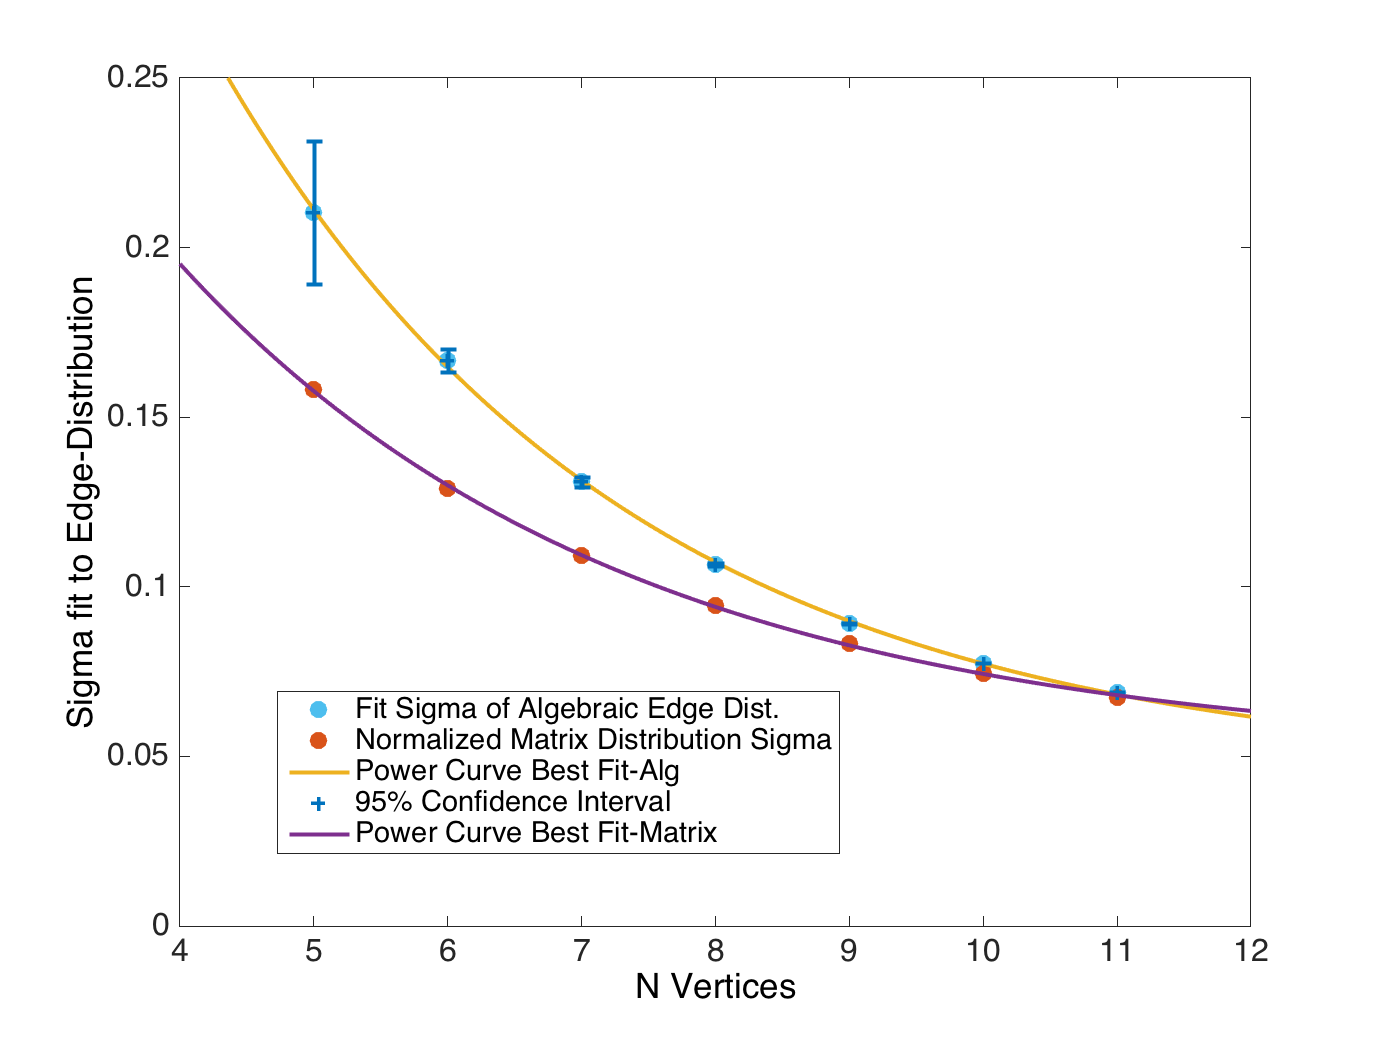
\includegraphics[width=\textwidth]{decreasingsigmawithbinom}
\end{figure}

Note that the values appear to shrink in their disparity, a remarkable observation, which gives us an idea of how the two sets/distributions differ with respect to the number of edges they produce as a function of N.
However, fitting exponential functions to each muddles the question: are they converging or intersecting and diverging again?
Note that even a convergence doesn't tell us about other properties of the sets of graphs.
Similarity in the distribution of the number of edges (or connectivity) does not equate distributional symmetry.
However, what we can see is that the Gilbert graph generator models the number of edges successfully for values of $N \approx 11$, and for larger values it may or may not  mirror this distribution.

%----------------------------------------------------------------------------------

\section{Specifically Disadvantaging Highly Automorphic Graphs}

Dominant models of random graph generation specifically preference graphs with fewer non-trivial automorphisms over graphs that have many automorphisms. 
This flaw is most glaring when discussing average or worst case running time over the `random' class of graphs.
Many algorithms make exciting claims about their performance on `random' graphs, but
we will show how theoretical and practical analysis of performance changes dramatically under different random graph generators.

\subsection{Two Quick Justifications}

To get an initial sense of this problem, we will first examine the relative probabilities of selecting a Co-Cycles graph from the set of graphs of size 10.
Since we know all 116 Co-Cycles graphs over 10 vertices, we can (without much computational effort) calculate the relative probabilities of generating a Co-Cycles graph under the standard (Gilbert) model and under the idealized model.
The results are not shocking, but a notable difference is apparent:
$$P(CoCycles(G) | G \in Gilbert) = \frac{\sum_{g \in CoCycles}^{116}M_{Reps}(g)}{N Matrices} = \frac{260820000}{3.5184 \times 10^{13}} = 7.4130 \times 10^{-6}$$
$$P(CoCycles(G) | G \in Gilbert) = \frac{N CoCycles Graphs}{N Graphs} = \frac{116}{12005168} = 9.6625 \times 10^{-6}$$

Though these are not exorbitent differences, it should be noted that there is a difference of 23\%, meaning that by using a Gilbert random graph generator, you are 23\% less likely to observe a co-cycles graph as a result of generating one random graph than you would be via an idealized generator.
In this case, the difference between the generators is clearly appreciable, but not severely limiting.

As a second example, we will compare the most and least likely graphs to be observed under either random graph model.
In an idealized random graph generator, all graphs have equal probability of being selected.
Thus, the ratio of the most likely to least likely is exactly 1.

In a Gilbert random graph generator (abstracting over p, as discussed earlier), graphs that are fully automorphic (where the automorphism set contains all one-to-one mappings), are the least likely to occur.
One such graph is the fully connected graph, or the complete graph ($K_N$).
This is simply because the number of matrices which represent them is given by $M_{Reps}$, and the probability of selecting a the complete graph is thus:
$$P(G = K_N | G \in Gilbert) =  \frac{M_{Reps}(K_N)}{NMatrices} = \frac{N! / |Aut(K_N)|}{2^{.5N(N-1)}} = \frac{N! / N!}{2^{.5N(N-1)}} = \frac{1}{2^{.5N(N-1)}}$$
However, if we examine a graph with only the trivial automorphism ($G_{TA}$):
$$P(G = G_{TA} | G \in Gilbert) =  \frac{M_{Reps}(G_{TA})}{NMatrices} = \frac{N! / |Aut(G_{TA})|}{2^{.5N(N-1)}} = \frac{N! / 1}{2^{.5N(N-1)}} = \frac{N!}{2^{.5N(N-1)}}$$
Thus, the ratio of these probabilities is always going to be $N!$.

These two examples give us a really important message: the difference between the Gilbert and Ideal models is frequently substantive, but its effects can be mild (as in the case of co-cycles graphs), or extreme (as in the case of selecting a perfectly automorphic graph).
What largely determines the degree of this distortion is the \emph{average number of automorphisms in the set that is being examined}. 
The larger this number, the more distortionary the Gilbert Model is when compared to the Idealized model.

\subsection{Theoretical Average Case Comparison}

Consider a standard canonical labeling algorithm.
This algorithm has two abstract components, one which correctly places vertexes into Similar Vertex Sets (SVS), and another which finds a canonical labeling given an accurate SVS partition.
If we take the first part of this algorithm as given, and assume that it can be computed in polynomial time (a reasonable assumption, as discussed in the section on SVS), then the running time of the algorithm is contingent upon the number of matrices we need to evaluate against some canonical property.
One common property for canonization is selecting the adjacency matrix which is the lexicographically smallest (or largest) representation of the graph.
It is reasonable to assume that the second half of the algorithm dominates the running time of the overall algorithm, as it is the piece that is inherently exponential based on the number of representations of the matrix.
Thus,  we can express the running time of the overall algorithm in terms of $O(|Aut(G)|)$, as this is the number of possible labelings we will have to examine to find our canonical one.

The selection of this simplified algorithm for analysis is not an accident: we have chosen it because the number of matrix representations ($M_{rep}(G)$) for a given graph $G$ is $\frac{N!}{|Aut(G)|}$.
Thus, if we are considering the average running time of this canonization algorithm ($\xoverline{T}_{Gilbert}$) over the set of all graph instances ($G_{Inst} = G(A)$ for $A \in \{\{0,1\}^{N \times N}\}$) (i.e. using the standard models for random graph generation), we come to different conclusions if we consider the set of possible graphs $G_{Inst}$, versus if we consider the set of all graphs as algebraic structural objects ($G_{Alg}$).
$$O(\xoverline{T}_{Gilbert}) = \frac{ \sum_{g \in G_{Inst}} O(T(g))}{|G_{Inst}|}$$
$$O(\xoverline{T}_{Gilbert}) = \frac{ \sum_{g \in G_{Alg}} O(T(g)) * M_{Reps}(g)}{|G_{Inst}|}$$
$$O(\xoverline{T}_{Gilbert}) = \frac{ \sum_{g \in G_{Alg}}  |Aut(g)| * \frac{N!}{|Aut(g)|}}{|G_{Inst}|}$$
$$O(\xoverline{T}_{Gilbert}) = \frac{ \sum_{g \in G_{Alg}}  N!}{2^{.5(N^2 - N)}}$$
$$O(\xoverline{T}_{Gilbert}) = \frac{ |G_{Alg}| * N!}{2^{.5(N^2 - N)}}$$

This property might not look like it tells us much, but we can actually approximate what it looks like for different values of N, since we have the frist nineteen values of this sequence from OEIS sequence A000088 CITE.
This data is shown below.
CITE

However, if we attempted to select a graph from the set of all graphs of that size, we would find that: 
$$\xoverline{T}_{Ideal} = \frac{ \sum_{g \in G_{Alg}}  O(T(g)) }{|G_{Alg}|}$$
$$\xoverline{T}_{Ideal} = \frac{ \sum_{g \in G_{Alg}}  |Aut(g)|}{|G_{Alg}|}$$
$$\xoverline{T}_{Ideal} = \text{Average Number of Automorphisms over Graphs}$$

Some sample numbers to give you the scale of these disparities is given below \cite{erdosreyni}.

The takeaway here is that specifically disadvantaging a class of graphs (namely highly automorphic graphs) warps our analysis of running time in a substantive way, not only for fringe algorithms, but for well studied algorithms too.
We can show this through the theoretical proof as shown above, but we can also show it through data describing actual algorithm performance.

\subsection{Practical Average Case Comparison}

The NAUTY package, written in CITE by CITE, is one of the quickest algorithms for canonical labeling CITE.
Though its performance is weaker on some graphs (like the Miyazaki, for example), in general, its canonical labeling algorithm is widely regarded and frequently used.

I ran the NAUTY canonization algorithm on batches of graphs with different numbers of vertices.
To generate the first sets of batches, I randomly selected graphs using the Gilbert model with probability 1/2, and varying values of N.
To generate the second batch, I first set N, then generated a random variable M to describe the number of edges (also with internal binomial probability 1/2), then selected with uniform probability from the set of all graphs with N vertices and M edges.
I ran each batch set ten times, to get a scatterplot describing the time complexity growth, and understand its variance.
The logarithmic graph of my results is shown below.  [CITE].

We can see from these figures that not only does NAUTY have slower performance on `Idealized' random graphs, but its running time increases at a higher constant value.
If we set these numbers to a log-lin regression, we see that this growth rate is heavily supported by the data.

Both in theory and in practice, distinguishing between 'random graph' and `random graph instance' has significant implications.
It is very possible that misuse of the Gilbert model has understated the true average and worst case time complexity for a number of algorithms.

\subsection{Should We Never Use the Gilbert Model?}

The short answer to this question is no, the Gilbert model is remains relevant (even dominant) even when we embrace these flaws.
The primary argument for the Gilbert model is not its application to questions of theory, \emph{but questions of practice and natural occurrence}.
Most applications of graph theory to world problems are based around structures that are naturally arising, without centralized planing or design.
It is much more likely that some graph that is found in the world will be non-automorphic than have some kind of inherent and difficult to describe complexity.
This is because if we look at graph building as a process [CITE GILBERT], or as a probabilistic construction [CITE EDRODS], then some outcomes are more likely than others.
This is well in line with the pervasive assumptions of the Gilbert model.

Rather, what we have been criticizing is the \emph{application} of the Gilbert model to questions about theoretical algorithmic complexity.
In graph theory, we hold a meaningful distinction between graphs and graph instances, a distinction only made at the theoretical level.
It is thus inappropriate to use a model which ignores this distinction, and ignores it in such a way as to specifically disadvantage certain classes of graphs.
This allows theoretical arguments about graph algorithms to underweight what we consider `hard' cases, and overweight what we would generally consider `easy' cases.

This distinction is important.
In practice, graphs that arise in the world are likely to be selected randomly from the set of graph instances.
However, in graph theory, where we consider isomorphic graph instances to be fundamentally equivalent, the assumptions of the Gilbert model are antithetical to other assumptions of graph theoretic research.

\section{Measuring and Comparing Random Graph Models}

Our mandate suddenly becomes: `well, what can we do which is better?'
Establishing an intuition to answer this question requires us first to understand what we would think of as `ideal', and see if we can approach that model.

\subsection{An Ideal Random Graph Model}
To allow our comparisons to be explicit, we will use the same nomenclature to describe an idealized generator as we do with the Gilbert model, so that they are directly comparable.
Thus, our ideal random graph model will take two input parameters, N and p, where p describes the probability of getting any given edge existing.
Note that this explicitly breaks from the idea of edge independence that is assumed in the Gilbert model.
Rather, we are assuming that the probability of any given edge existing is p if we have no knowledge about the rest of the graph.
We will define our `Ideal' generator as one which first selects a number of edges M from the binomial distribution with $E_{Max}$ trials and trial success probability $p$.
After selecting M as an observation from this random distribution, we will select a graph from the set of all graphs of N vertices and M edges with uniform probability.
To accomplish this task, we will enumerate all graphs of that size, and select from that fully defined set.

The flaw in this scheme is obvious.
Our `Ideal' generator is only possible by this methodology so long as you can enumerate all graphs of a given size.
There are 24637809253125004524383007491432768 non-isomorphic graphs over 19 vertices, so this is not remotely sustainable methodology for a random generator.
If we cannot rely on an ideal graph generator, are we doomed to stick with the Gilbert model?
Or, could we create a model that is better than the Gilbert model (closer to our ideal), while being computationally reasonable?

\subsection{An Equivalent Ideal Random Graph Model}

Another way to view our equivalent random graph model is as a overlaid construction on top of a standard, Gilbert, random graph model.
Since we know that the Gilbert random graph model produces a graph with a probability proportional to its number of automorphisms, we can actually create a random graph generator which is equivalent to our idealized model by systematically throwing out graphs with probability inverse to their probability of showing up.
The algorithm which generates to this model is not guaranteed to halt, but does simulate our idealized random graph generator, even over large values of N.

\begin{lstlisting}[frame=single]
while true:
	g = gilbertRandomGraph(N, P)
	na = |Aut(g)|
	p = Math.rand(0, 1)
	if (p < (na / N!))
		return g
\end{lstlisting}

Here we find a gilbert random graph, and calculate the number of automorphisms that it has.
That gives us knowledge of how many times we would expect it to occur in a sample of $2^{E_{max}}$ random graph instances, namely $N! / na$ times.
Thus, we weight any randomly observed random graph instance by the inverse of this value.
This equalizes the probability of getting any graph, regardless of its number of automorphisms.

This methodology is, unfortunately, equally unsustainable.
This is an example of a geometric process, where we will have to go a certain number of trials before finding a success and stopping. 
The probability of a success on any given trial is $p = \frac{|G_{alg}|}{|G_{inst}|}$, which approximates the $p = fact^{-1}(N) = \frac{1}{N!}$ growth function.
Thus, for even a small number of vertices, the expected number of trials that need to be generated before a success is found is very large, as it is given by $1/p = N!$. 
For example, if $N=10$, we would expect to have to examine 3.6 million graphs before finding one which is returned successfully.

This too, is not a sustainable methodology for random graph generation.

\subsection{Establishing a Methodology for Random Graph Generator Evaluation}

So what can we do that is better?
Answering that question required some really deliberate thought.
I knew lots about what I didn't want to do:
\begin{itemize}
\item{I didn't want to use subjective measures to support one random graph generator over another.}
\item{I didn't want to write generators and then use collected data to support them.}
\item{I didn't want to focus in on singular ways of looking at the quality of the graphs that I generated.}
\item{I didn't want to allow my own intellect and lack of creativity be a limiting step on the way to a better generator.}
The process that I decided on attempted to address all of these concerns, and was designed to avoid the pitfalls of bad computer science: overfitting, statistic selection, and rigidity.
\end{itemize}

I decided on a wide portfolio of statistics each of which is calculated over a sets of graphs.
These statistics are inherently heuristic, but each attempts to capture some property of the graphs that are generated, or some property of how the set looks as a whole.
Each of the statistics I decided on is meant to describe some property of a set of graphs, but it does not establish an `idealized' or theoretical value for that statistic.
Though for several of these metrics we know how to express the ideal/expected probability, that is not always the case (or not always known to be the case0.
These metrics serve as a way for us to identify and name ways that random graph generators fail us, and challenge us to do better, to compare a proposed solution to an ideal or standard solution in quantifiable and concrete terms.

The set metrics is described in the next section, and they vary in computational complexity and broad descriptiveness.
I set up a (pardon the brag) BEAUTIFUL system for calculating these statistics over arbitrary datasets.
I created an idealized random generator (as described above), and a Gilbert random generator, and verified the accuracy of the results produced through this computational system over the initial results from each.

Most importantly, I set up these metrics, this system, and the baseline Gilbert/Ideal metric values before I wrote a line of code which randomly generated graphs.
This is really important to me, because it frees the results of this work from the publication and statistic selection bias that plagues research everywhere.

\subsection{Graph Set Metrics}
Below are the metrics that I compared across graph sets generated by different random graph generation procedures.
Though I calculated some more statistics for personal use and discovery, the ones included below are the `single result' statistics.
Others were distributional properties that were not easily captured and compared (except through distributional goodness of fit tests, which only give us an idea of alikeness, not of directed difference).
The reliance on singular metrics as a means of comparison allows us to evaluate systems of random graph generation automatically, and come up with similarity tests that are divorced from our intuition and hypotheses.

Described below are each of the metrics that are calculated over every set of random graphs that were generated.
Each is labeled a statistic (implying a singular value used to judge the generator) or a distribution (connoting that it was not used in the systematized evaluation of generators).
Each is listed under its acronym, which can be found throughout my code and tests. 

\subsection{Graph Set Metric Reference, Coding and Description}

\begin{itemize}

\item{ADIAM - Set Statistic - Average Graph Diameter - Take the diameter of each graph, and average over all graphs in the set}
\item{ADSM - Set Statistic - Average Degree Sequence Mean - take the mean of degree sequence of each graph, and average that across all graphs}
\item{ADSMD - Set Statistic - Average Degree Sequence Median - take the median of the degree sequence of each graph, then average that across all graphs}
\item{ADSMN - Set Statistic - Average Degree Sequence Minimum - take the degree of the least connected node in each graph, then average that across all graphs}
\item{ADSMX - Set Statistic - Average Degree Sequence Maximum - take the degree of the most connected node in each graph, then average that across all graphs}
\item{ADSR - Set Statistic - Average Degree Sequence Range  (i.e. Find the difference in degree between the most and least connected node, and average over all graphs in the set}
\item{ADSV - Set Statistic - Average Degree Sequence Variance - take the variance of the degree sequence of the graph, then average across all graphs}
\item{ALNA - Set Statistic - Average of the Logarithm of the Number of Automorphisms - Find the number of automorphisms that each graph has within the set, take the logarithm of each, then average across the logged results}
\item{ANA - Set Statistic - Average Number of Automorphisms - find the number of automorphisms for each graph, then average that across the set}
\item{ANCC - Set Statistic - Average Number of Connected Components - take the number of connected components of each graph in the set, then average across all of them}
\item{ANQUAD - Set Statistic - Average Number of Quadrilaterals - The Average number of non-trivial (non-edge repeating) quadrilaterals across all graph instances within the graph set.}
\item{ANR - Set Statistic - Average Number of Repeats - The average graph, when selected from the set in question, will have this expected number of equivalent instances in the set}
\item{ANTRI - Set Statistic - Average Number of Triangles - The Average number of triangles across all graph instances within the graph set.}
\item{CP - Subset - Co-Cycles Graphs - The intersection between the set of all $V=10$ co-cycles graphs and the given set}
\item{DIAMV - Set Statistic - Variance in the Diameter of Graphs - calculate the diameter of each graph, and calculate the variance of the set as a whole}
\item{DSMDV - Set Statistic - Degree Sequence Median Variance - Take the median degree of each graph, and calculate the variance over all graphs in the set}
\item{DSMNV - Set Statistic - Degree Sequence Minimum Variance - Take the minimum degree of each graph, and calculate the variance over all graphs in the set}
\item{DSMV - Set Statistic - Degree Sequence Mean Variance - Take the mean degree of each graph, and calculate the variance over all graphs in the set}
\item{DSMXV - Set Statistic - Degree Sequence Maximum Variance - Take the maximum degree of each graph, and calculate the variance over all graphs in the set}
\item{DSVV - Set Statistic - Degree Sequence Variance Variance - Take the variance of the degree sequence of each graph, and calculate the variance over all graphs in the set}
\item{FC - Set Property - Frequency Count - The number of isomorphic graph instances associated with each one of the graphs in the set}
\item{FFC - Set Distribution Counts - Frequency Count Counts - The counts that correspond to FFVs, the frequency with which graphs show up in our random set}
\item{FFV - Set Distribution Bins - Frequency Count Bins - The discrete values for which there exist graphs in our set that poses that number of instances in the set, this is really just a bin count for FC}
\item{MLNA - Set Statistic - Median of the Logarithm of the Number of Automorphisms - Find the number of automorphisms that each graph has within the set, take the logarithm of each, then find the median across the logged results}
\item{MNR - Set Statistic - Maximum Number of Repeats - The graph in the set that was selected the most times was selected this many times}
\item{NA - Graph Statistic - Number of Automorphisms - Counts the number of automorphisms that a graph has by finding the number of unique matrices that describe a graph}
\item{NAB - Set Distribution Bins - Number of Automorphisms Bins - The unique values of NA, to provide histogram alongside NAC}
\item{NAC - Set Distribution Counts - Number of Automorphisms Counts - The counts of the NAB, as in a histogram}
\item{NCCV - Set Statistic - Variance in the Number of Connected Components - take the number of connected components of each graph in the set, then take the variance of the set}
\item{NCP - Set Statistic - Number of Co-Cycles graphs - Same as Co-cycles graphs, this only applies to graphs of size 10 and larger, counts the number of Co-Cycles graphs (which tend to be highly automorphic) in the overall set of graphs}
\item{NE - Set Statistic - Number of Edges - the average number of edges in the graph set. This should be the same across generators, as we are specifying $p$, and asking for a large sample size}
\item{NR - Set Statistic - Number of Regular Graphs - the number of regular graphs in the graphset}
\item{NUG - Set Statistic - Number of Unique Graphs - The proportion of graphs within the set that are only generated once}
\item{ODSPL - Set Statistic - Overall Degree Sequence Poisson Distribution Lambda  - Find the set of all of the degrees of all of the graph, then fit a poisson distribution to this distribution. Report the lambda that defines this poisson distribution}
\item{PCONN - Set Statistic - Probability of Connectivity - take the number of fully connected graphs, and divide by the total number of graphs in the set}
\item{PDL - Set Statistic - Poisson Distribution Lambda - Take the distribution of the number of times that each graph is represented by an instance within a graph set, and set this distribution fit to a poisson distribution, reporting its lambda}
\item{PQRA - Set Statistic - Percentage Quazi-Regular A - Percentage of graphs where the degree sequence range is less than or equal to 1}
\item{PQRB - Set Statistic - Percentage Quazi-Regular B - Percentage of graphs where the degree sequence range is less than or equal to 2}
\item{PQRC - Set Statistic - Percentage Quazi-Regular C - Percentage of graphs where the degree sequence range is less than or equal to $sqrt(N)$}
\item{PTRIL - Set Statistic - Probability Triangle-less - the Probability that a graph instance selected randomly from the graph set is triangle-less.}
\item{SQNR - Set Statistic - Sum of Squared Number of Repeats - A measure of how dispersed the distribution is, calculated as $FFC \dot (FFV^2) / nGraphs$}
\item{UG - Set Property - Unique Graphs - The canonical form of all of the graph set's graphs, with duplicates removed (if they existed)}
\item{VLNA - Set Statistic - Variance of the Logarithm of the Number of Automorphisms - Find the number of automorphisms that each graph has within the set, take the logarithm of each, then find the variance of the logged results}
\end{itemize}

\subsection{Establishing Baselines for Graph Set Metrics}

Once we set up these metrics, we need to find a way to systematically compare them within our desired context: building a random graph generator which models an idealized random graph generator.
To do this, I established baseline understandings for each one of the metrics, over a problem `domain':
\begin{itemize}
\item{Number of Graphs - I decided to operate over sets of 1000 graphs.  It allowed us to get reasonable numbers for standard deviations and not use an excess of CPU time}
\item{Number of Vertices - I baselined the metrics over graphs of size 4 to size 10.  This allowed us to see what the metrics looked like on an overrepresented graph set, and on a sample set.}
\item{Probability of Edges - I used p from the set $[.1, .2, .3, .4, .5, .6, .7, .8, .9]$. I figured that focusing on sparse, dense or intermediate graphs might introduce biases that I hadn't accounted for, so I decided for the most generic set possible.}
\item{Number of Trials - For each one of these baseline scenarios, I performed 30 trials}
\end{itemize}

Thus, in the end, there were $2 \times 9 \times 7 \times 30 = 2780$ sets of 1000 graphs that were used to create our baseline metrics.

For each one of the statistics we calculated the mean and standard deviation of the sampled metrics over both algorithms.
That resulted in two sample means and sample standard deviations, for the ideal and gilbert graph models: $\xoverline{x_I}, \xoverline{x_G}, s_I$ and $s_G$. 
Using these values, I came up with a simple and intuitive way to measure a new random graph generator, given its value for $\xoverline{x_N}$ and $s_N$ and the number of samples that were used to compute each, $n_N$.
This methodology compares the t values in two tests of significance for two unknown means and unknown standard deviations.
In a test of unequal unknown means and standard deviations, the slightly modified t-statistic is given by:
$$T(A, B) = T(\xoverline{x_A}, \xoverline{x_B}, s_A, s_B, n_A, n_B) = \frac{|\xoverline{x_A} - \xoverline{x_B}|}{\sqrt{(s_A^2 / n_A + s_B^2 / n_B}} $$
And our scoring mechanism for a metric and generator is given by:
$$ \text{Score for Metric M} = -1 * \text{min} \bigg[ \ln \Big( \frac{T_M(I, N)}{T_M(I, G)} + e^{-10} \Big), 10 \bigg] $$
Lets break down this scoring mechanism:
\begin{itemize}
\item{First off, $T_M(A, B)$ is strictly greater than or equal to zero (and all of our metrics have non-zero $T_M(I, G)$ values), thus the fraction in the logarithm is defined and in the range $[0, \infty)$. When we add $e^{-10}$, we shift that range up to $[e^{-10}, \infty)$, meaning that the logarithm's value will be bounded between $[-10, \infty)$ }
\item{Next, we take the minimum of this score and 10, to bound the individual score between $[-10, 10]$.}
\item{Finally, we invert the values with a -1, so that a score of -10 corresponds to a metric where the new random graph generator performs incredibly poorly, while 10 corresponds to a metric where the new random graph generator is indistinguishable from ideal (with respect to the differences setup by the baselines).}
\item{The resulting metric has the helpful property that the baseline metric is at (or ever so slightly below) 0, so that a score of 0 marks an equivalence in quality to the Gilbert random generator.}
\end{itemize}
Once we calculate individual metrics, we can calculate the score for a generator as the sum over the number of metrics that are calculated for it, which includes multiple values of p and n:
$$ \text{Score for Generator} = \frac{1}{N_{Metrics}} \times \sum_m^{Metrics} Score_m $$
in this metric, higher scores are better and a score of 0 corresponds to a generator that is exactly as bad as the Gilbert Generator.

This is a good mechanism because it scores a value on a metric based on how close it is to the ideal mean, but also compares any deviancy to the deviancy observed between the ideal and standard (Gilbert) generators.

\subsection{Finding Data on Graph Set Metrics and Scores}

The baselines for the graph set metrics are all stored in one file for convenience (Thesis/Matlab/Alternative Generator/Data/baselineMetrics.mat).
As mentioned above, they are for the tenth-probabilities, over graphs of size 4 to 10.
The baselined metrics were constructed using thirty random trials, each containing 1000 random graphs.
In the baseline file, the mean, standard deviation and number of samples is given.

An appendix to this thesis lists the graph set baselined metrics, along with their associated uncertainties, for all values of N and P.
Since there were 7 tested values of N, and 9 tested values of P, and 35 metrics, over two different generators for random graphs, there are a total of approximately 4,000 component statistics in this baseline file.

\subsection{Examining the Difference between Gilbert and Ideal Baselines}

The differences between the Gilbert random graph generator and the Idealized generator are on display in the visual examination of the metrics described above.
To see the full range of differences, and the full set of charts that were generated to supply some of these examples, please check out my code on github.
These files in particular are stored at /Thesis/Matlab/alternative generator/analysis.

In this section, we will summarize the broad tendencies (and larger deviations) that we see between the two models.
There are six different categories that I placed each of the metrics within, describing six different patterns of difference.
The graphs used for this section should be taken with a grain of salt: in our baselines, we perform 30x the number of trials that generated these graphs, so they certainly are prone to more vertical uncertainty.
However, we have graphed many more values of $p$, so these graphs can better show how the baselines change across values of $p$, not only see their absolute differences.

\subsection*{Identical - ADSMD, ADSMN, ANQUAD, DSMV, NE, ODSPL} 
Some of the metrics were indistinguishable between the two random graph generators.
Approximately six of the thirty-five metrics behaved indistinguishably between the Gilbert and Idealized random graph generators.
An example is shown in the figure below, which describes the number of quadrilaterals in a graph set for various values of $p$ (the graphs were all of size 10, and there were 1000 of them represented by each dot).

\begin{figure}[h]
\label{fig:anquad10}
\caption{}
\centering
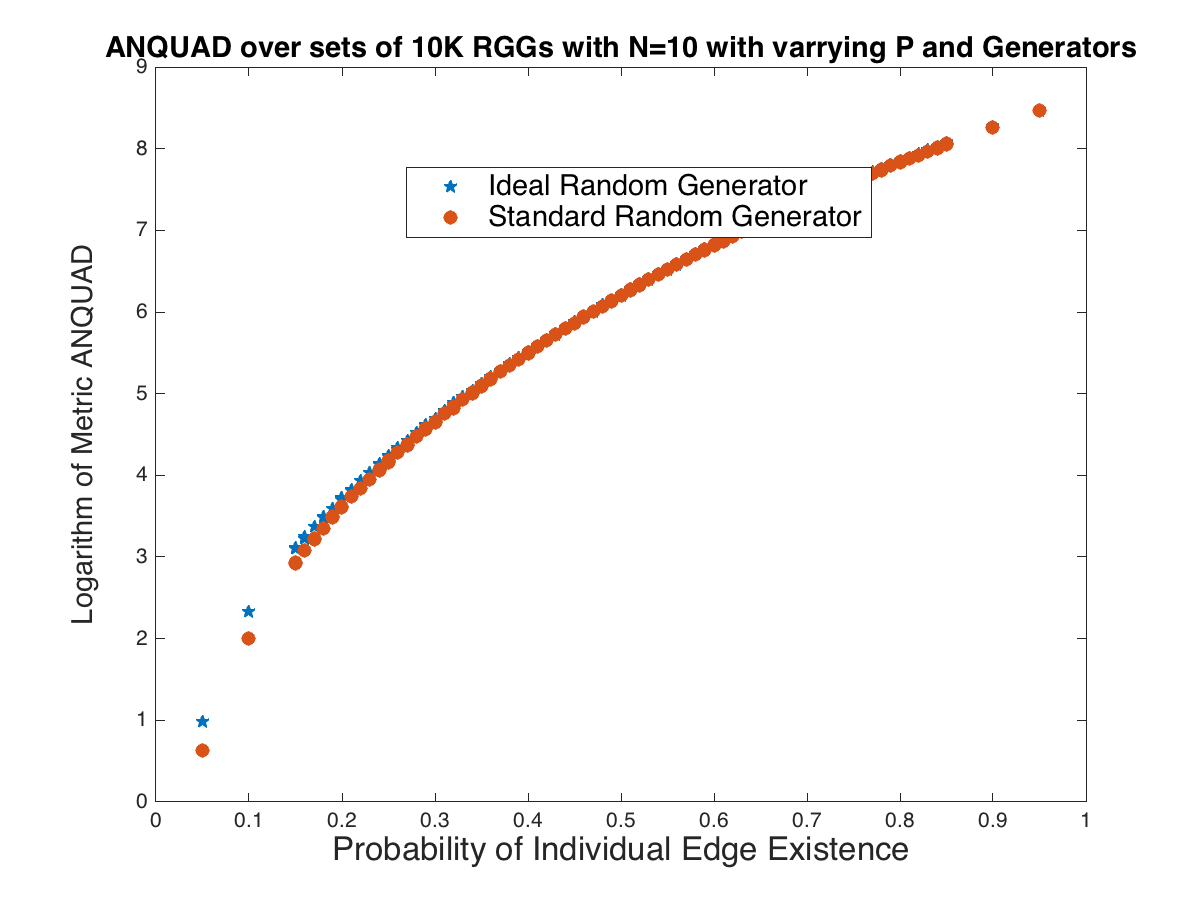
\includegraphics[width=\textwidth]{ANQUAD-10}
\end{figure}

\subsection*{Height Different - ADIAM, ADSMX, ANA, ANCC, ANR, ANTRI, DIAMV, MLNA, NCCV, NUG, PCONN, PDL, PQRA, PQRB, PQRC, SQNR} 
Many of the metrics had the same broad patterns between 

\begin{figure}[h]
\label{fig:sqnr7}
\caption{}
\centering
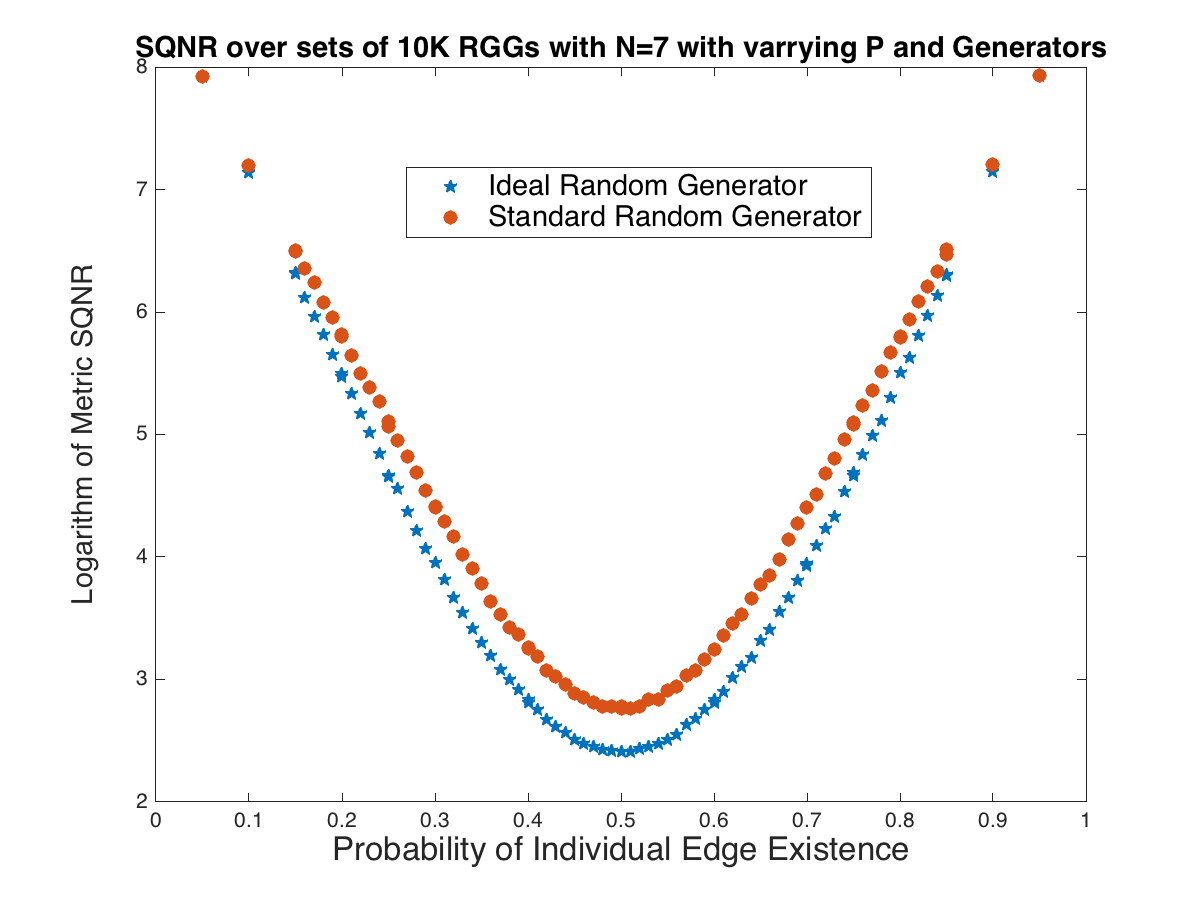
\includegraphics[width=\textwidth]{SQNR-7}
\end{figure}

\subsection*{Not Enough Data - NCP}
For one metric, there was consistently not enough data to calculate it or any comparison between two random graph generators.
It shouldn't come as a surprise that that metric is NCP, the number of Co-Paths (or Co-Cycles) graphs in the graph set. 
Since there was consistently not enough data to establish a baseline, you will find that most of the time NCP is zeroed out, not by some choice of mine, but becuase of the way I have set up  my scoring mechanism.

\subsection*{Crossover - ADSR, ADSV, NCCV, PTRIL, VLNA}

\begin{figure}[h]
\label{fig:diamv5}
\caption{}
\centering
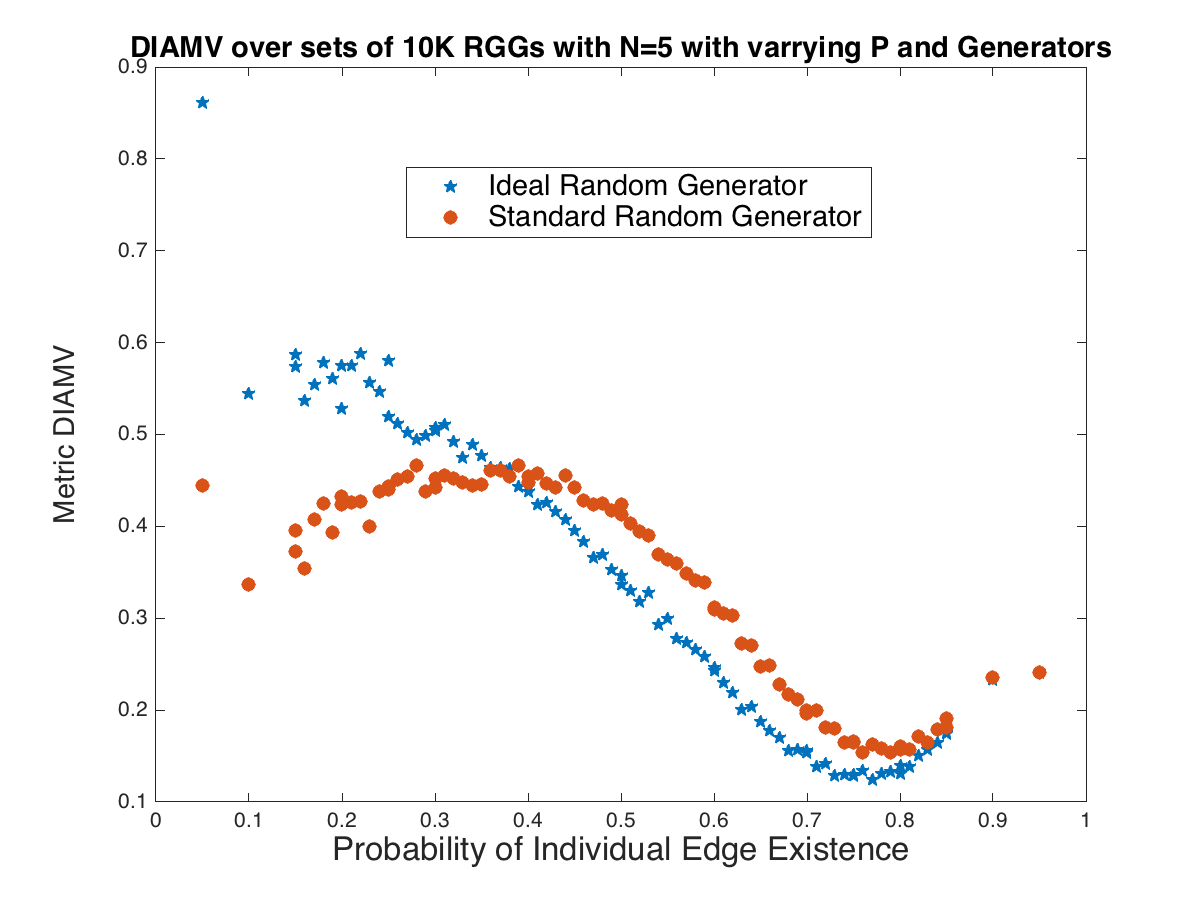
\includegraphics[width=\textwidth]{DIAMV-5}
\end{figure}

\begin{figure}[h]
\label{fig:vlna6}
\caption{}
\centering
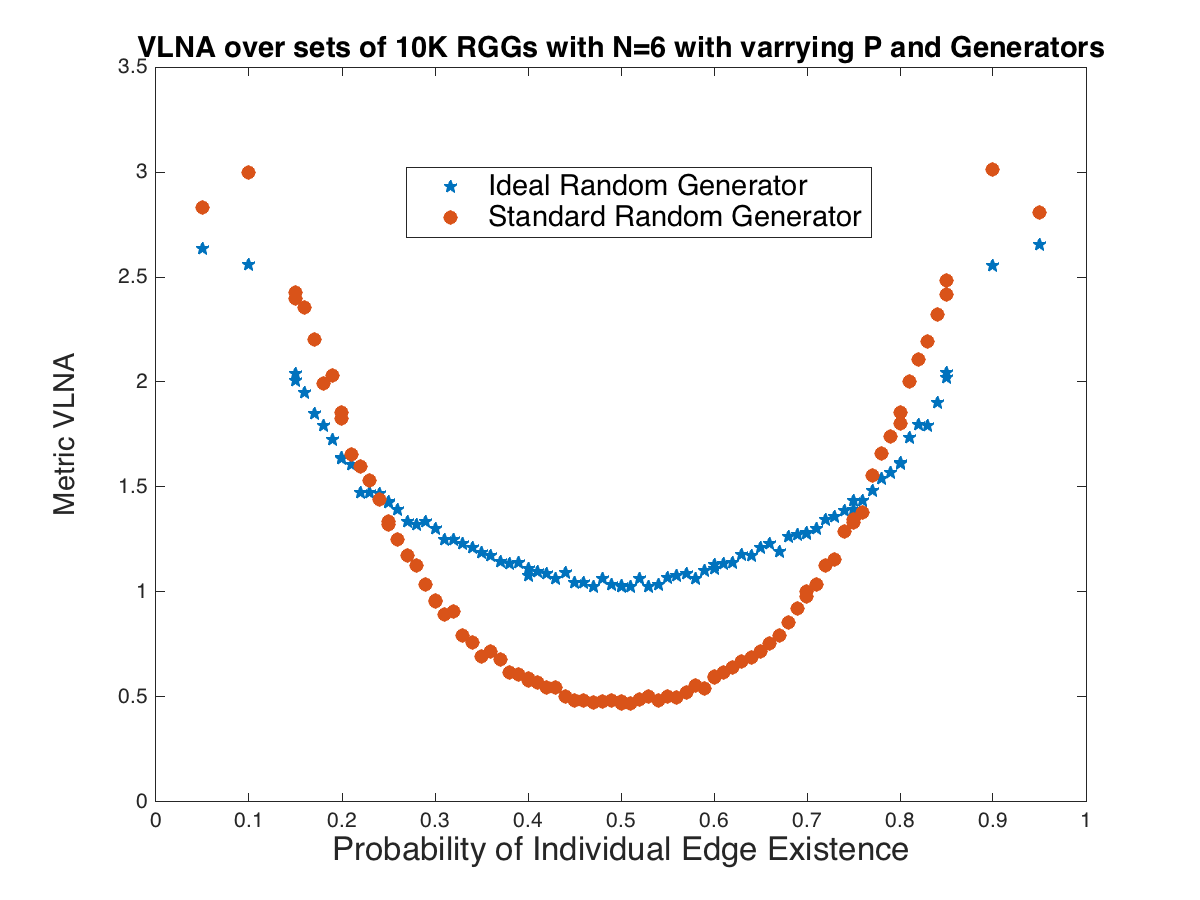
\includegraphics[width=\textwidth]{VLNA-6}
\end{figure}


\subsection*{Shape Different - ALNA, DIAMV, DSMDV, DSMNV, DSMXV, DSVV, MNR, NR}

\begin{figure}[h]
\label{fig:dsmxv10}
\caption{}
\centering
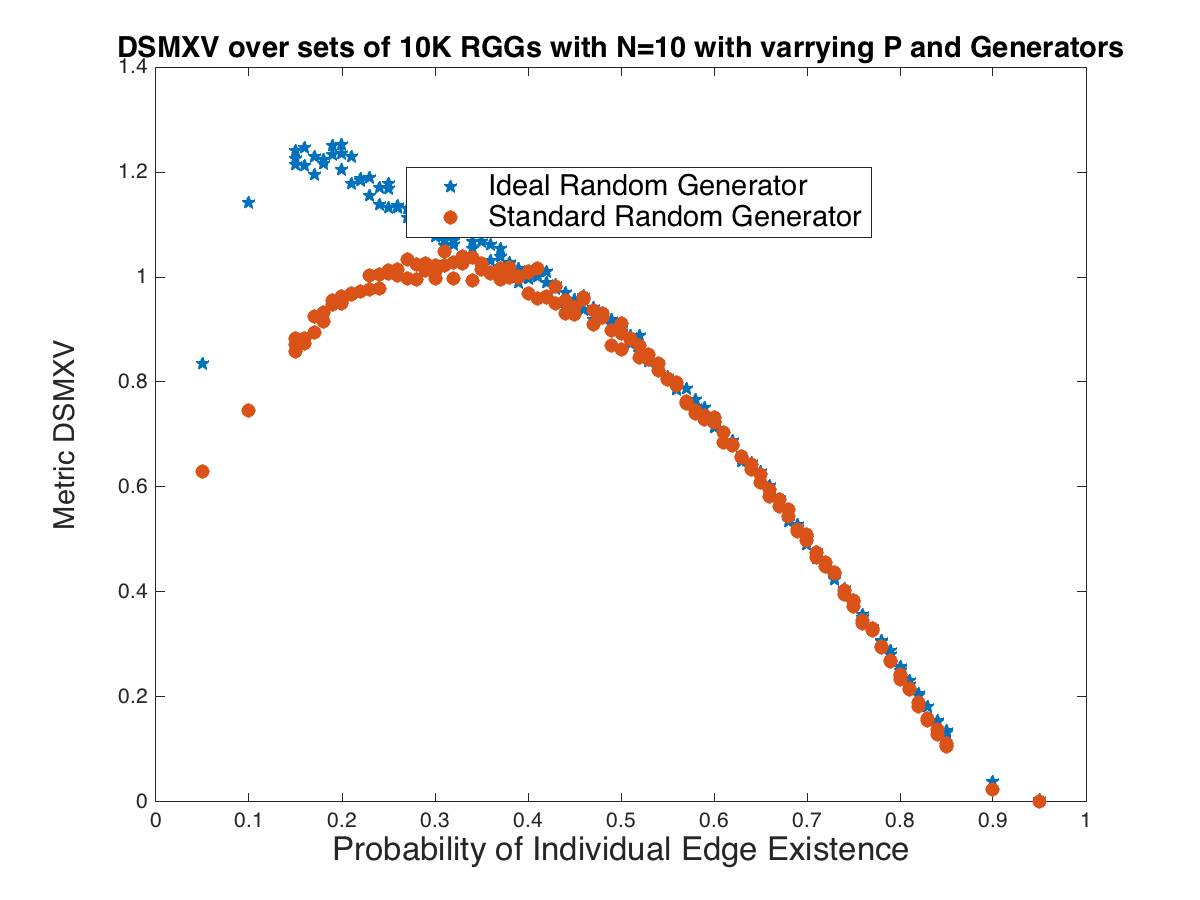
\includegraphics[width=\textwidth]{DSMXV-10}
\end{figure}

\begin{figure}[h]
\label{fig:adiam9}
\caption{}
\centering
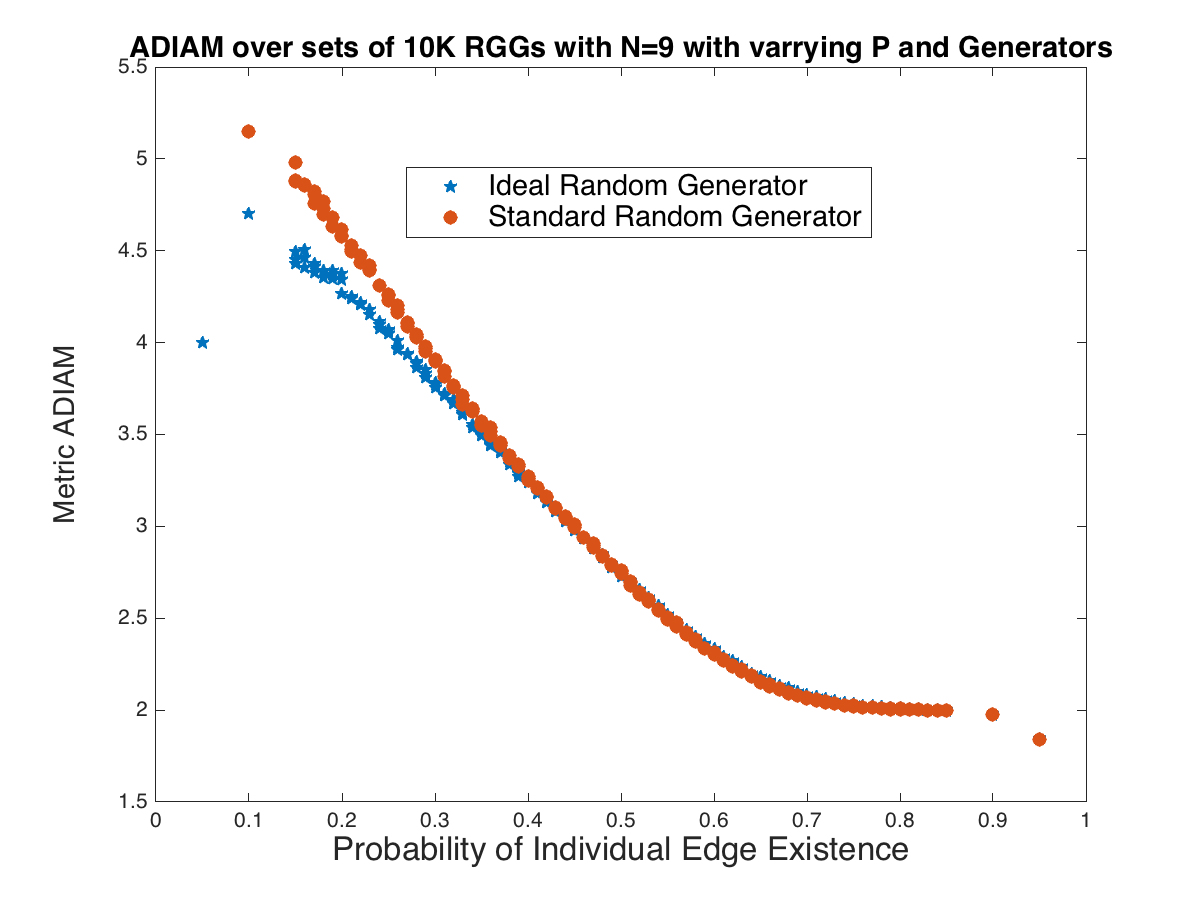
\includegraphics[width=\textwidth]{ADIAM-9}
\end{figure}


\section{Alternative Ideas for Random Graph Modeling and Creation}

Now that we have a mechanism for quantifiably adjudicating the quality of a proposed random graph generator, we are tasked with creating different ideas for random graph generation and evaluating them on this basis.
Discussed below are each of the algorithms that I built for Random Graph Generation and Processing.
They are not presented in any particular order.
Each is prefixed by the string that it is represented as/by throughout the code.

\subsection{MinusOne - A Weighted Automorphic Subgraph Generator}

MinusOne has a simple methodology.
If you are generating a graph with $N$ vertices and with probability of edge creation $p$, start by creating a graph $H$ of size $N+1$ via the gilbert model.
Then, generate all $N+1$ of $H$'s single vertex deleted subgraphs, store each in a set we will call $VD(H)$.
Lets define an automorphic metric $AM$ which is defined by the following formula, finding the QSVSes, and take the product of the factorial of their sizes.
$$AM(g) = \prod_{i \;\in \;QSVSes(g)} |QSVS_i|$$
Finally, over each member of the set $g \in VD(H)$ calculate the automorphic metric, and select that graph with the probability:
$$P(g | H) = \frac{AM(g)}{\sum_{h_i}^{VD(H)} AM(h_i)}$$

\subsection{MinusOneA - Less Automorphic Version of MinusOne}

MinusOneA has a methodology with closely matches that of MinusOne.
The only difference is the automorphic metric function, which is the logarithm of the one proposed above (plus a constant factor).
$$AM(g) = 1 + \log_2 \Big[{\prod_{i \;\in \;QSVSes(g)} |QSVS_i|} \Big]$$

\subsection{MinusOneB - Interspersing Some Gilbert Random Graphs}

MinusOneC has an identical methodology with closely matches that of MinusOne, with one caveat.
With a probability selected based on $p$, the algorithm chooses between picking a graph from a MinusOne distribution and a Gilbert distribution:
\[ MinusOneB(n, p) = \begin{cases} 
      Gilbert(n, p) & \text{if $rand < .5 * (p) * (1-p)$} \\
      MinusOne(n, p) & \text{otherwise} \\
   \end{cases}
\]

\subsection{MinusOneC - Less Automorphic Version of MinusOne}

MinusOneC has a methodology with closely matches that of MinusOne.
The only difference is the automorphic metric function, which is the square root of the one proposed above.
$$AM(g) = \sqrt{\prod_{i \;\in \;QSVSes(g)} |QSVS_i|}$$

\subsection{BuildingA - An Iterative Graph Generator}

Building Algorithms are processes by which edges are added individually to a matrix (given a `probability matrix'), and then a new probability matrix is generated from the current iteration of the formative graph.

\begin{lstlisting}[frame=single]
nEdges = binomalRandom(N, P)
A = zeros(N)
P = (ones(N) - eye(N))/(N*(N-1))
while nEdges > 0:
	A = addEdgeFromProbabilityMatrix(A, P)
	P = generateProbabilityMatrixFromPartialGraph(A)
	nEdges = nEdges - 1
\end{lstlisting}

From this, it is clear that the only place that one can really modify this algorithm is in the generation of the $P$ matrix from the partially generated graph $A$.
BuildingA used a simple algorithm to do this.
It created an edge metric $EM(v_i, v_j)$ to describe the odds of creating an edge between vertices $v_i$ and $v_j$ (here, $DS$ refers to the degree sequence of A as it exists at each iteration):
$$ EM(v_i, v_j, A) = (i - j  \neq 0) * (1 - A[i, j]) * \Big[ 1 + 2 max(DS) - DS[i] - DS[j] \Big] $$
And with the probability of selecting a given edge for creation being:
$$P(\,(v_i, v_j) \,| A) = EM(v_i, v_j, A) / \sum_{x = 1}^{N} \sum_{y = 1}^{N} EM(v_x, v_y, A)$$

\subsection{BuildingB - An Inverse Differential Graph Generator}

The BuildingB random graph generator operates identically to BuildingA, with a change in the individual edge metric $EM_A$:
$$ EM(v_i, v_j, A) = (i - j  \neq 0) * (1 - A[i, j]) * \Big[ 1 + 2 max(DS) + DS[i] + DS[j] \Big] $$

\subsection{Cloning Model}
One of the thoughts that I first had was on the way that Co-Cycles graphs tended to be highly automorphic, and the way that internal structure of each set within the SVSes was almost always fully automorphic.
Remember that a fully automorphic graph (or in this case, subset of vertices) means that within its self contained structure, there exists an automorphism which maps any one vertex to any other (not implying that all proposed mappings are automorphisms, but only that a mapping exists that pairs any pair of vertices within the set.
To try to create a model that is likely to produce this kind of internally reflective behavior, I broke the task of generating a graph down into two subtasks.
First, it creates K disjoint graphs, each of which is fully automorphic/similar, and with the total number of vertices over all of these smaller graphs equalling the target number of vertices the generator is looking to produce.
Then, it constructs a set of connections between each pair of the K subgraphs.
With fixed probabilities, it constructs these connections to be either fully symmetric (i.e. preserving symmetry for both the right and left hand side of the connection), partially symmetric (just preserving one side's symmetry), or asymmetric (differentiating both sides).

This model was not successful at producing graphs which are broadly in line with the aims of the chapter (i.e. idealized random graphs), but it was very successful at producing co-cyclic graphs, with regularity far exceeding that of either generator. This initial attempt's results are detailed below, alongside some different results given different parameter values (for the fixed probability of edge symmetry creation.


\chapter{Further Questions}


\section{Reconstruction Hypothesis}

The Reconstruction Hypothesis is a claim in theoretical computer science that is very likely true, but has not been proven to be.
The hypothesis revolves around the notion of a `deck' of a graph $G$ with $N$ vertices.
The Deck of G ($Deck(G)$) is a (possibly multi-)set of $N$ graphs, each of size $N-1$, all of which are created by deleting one vertex from the graph G.

Two Decks $D_1$ and $D_2$ are said to be isomorphic if there exists a one to one mapping of their elements such that every graph $g_i \in D_1$ is mapped to an isomorphic graph $g_j \in D_2$.
The reconstruction hypothesis is the claim that two decks are isomorphic if and only if their graphs are isomorphic, or in formal terms:

$$ Deck(G) \cong Deck(H) \iff G \cong H$$

Though this hypothesis seems pretty iron clad, there is one known violation, two non-isomorphic graphs over two vertices have congruent decks. Can you find them? (hint: there are only two graphs over two vertices).
Thus the actual hypothesis only makes its claim for $N \geq 3$.
As we get to larger and larger values of $N$, it would seem that the hypothesis becomes harder to refute via a counter example, both because the amount of information that goes into the physical representation of the deck increases cubically, and because the unknown pieces of the graph shrink relative to the consistent amount provided by each card in the deck.

However, the nature of the hypothesis is so hard to verify, (and the number of graphs grows so large so quickly) that its verification has only been done up to graphs of 11 vertices, by McKay in 1999.

One would think, that with today's technology and resources, we ought be able to improve upon that bound, and increase N to 12 (or find a counterexample therein).
That is hopefully the site of some future work.

% ------------ Bibliography ----------------

% Adds all of the citations to the Paper, regardless of if they are used.
\nocite{*}

\bibliographystyle{plain}

\bibliography{bibliography}

% ------------ Appendices ----------------

\chapter*{Acknowledgments}

When I asked Professor Storer to supervise me on a thesis on the graph isomorphism problem, he was hesitant.
He only acquiesced when I persuaded him that my future was secure with a fantastic job, and that my primary objective was the pursuit of questions that were of nothing but personal interest to me.
In many respects, his skepticism proved well founded.

This work has been incredibly challenging, both in that the body of existing work on GI is so large, and in that few visible niches of it exist which are promising and not thoroughly explored.
Over the past year I have poured my time and energy into this project, and have found it unbelievably energizing to do so.
I have been thrilled to find interesting properties in problems surrounding GI, and have had an equal number of frustrations in finding that my results had been previously discovered.
Moreover, it has been illuminating to begin to understand a hidden world of graph theory which had before seemed either trivial or intractably complex.

I would like to thank Professor Storer for the initial bout of skepticism about this project, as it shaped this project and experience for the better.
But I would also like to thank him for the amount of advice and freedom that he has supported me with on this project.
It has kept me on track to focus on my real goal for the semester, which was to learn and grow.
I have learned advanced techniques in GPU calculation, proof techniques in abstract algebra, and gotten the chance to reason with established problems in new and interesting ways.
My skill set has been broadened by this project which has deeply challenged me and always kept me on my toes.

I would like to thank my advisors (Prfs. Storer, Di Lillo and Torrey), the Computer Science department, and my friends and family for all of the different kinds of support and encouragement that have brought me to successful completion of this project.

\chapter*{TL;DR}

Given a graph, count the number of closed paths (cycles) of every length that pass through each vertex in the graph.
It turns out that we can do this very quickly, relative to how much information it gives us.
Counting the number of cycles gives us a vector which describes a kind of local resonance, a description of the localized area around each vertex within the graph.
This idea can be transformed into a numerical property, called an invariant, which is highly information dense--able to describe differences between graphs (or vertices) with high probability, but not sufficient to verify that two graphs (or vertices) are the same.

There are many graphs, even over a small number of vertices, but the number is much larger if you consider different labelings of the same graph to be distinct.
This difference matters in many contexts, but is most evident through examining random graph generators, which treat different labelings of the same graph as if they are distinct graphs. 
This is not a problem in and of itself (it makes sense in many practical contexts), but it warps theoretic arguments about the runtime of algorithms over `random' graphs.
It turns out that making up our own random graph generators can actually improve upon this state of affairs in a quantifiable way.

\chapter*{An Open Source Project}

An interesting aspect of this thesis has been that I have placed every incremental iteration of my work online, through the git version control system and GitHub.
Every element, from my reading notes, to my mid-semester reports, to my code, results, and datasets: everything has been kept in a central repository, and every change has been committed and logged.
Alongside this choice, I have decided that every line of code I have written is open source and publicly available for use; licensed under the Creative Commons Attribution-ShareAlike 4.0 International License.

There are three reasons to make this thesis as an open source, version controlled work.
\begin{enumerate}
\item{
Research in academia is far too often done in the dark, and only once the conclusion has been drawn and sufficiently polished does the general public get to learn about it. 
This falsely represents scientific inquiry as a lightning bolt, a blinding and stark progression from correct idea to correct idea. 

In reality we all explore ideas that fail, we all have intuitions that turn out to be incorrect.
The reality of research is much more one of lightning's infinitesimally branching electrical charges (with eventual connection and brilliance). Though this report presents a well coordinated and rehearse set of conclusions, this is not a reflection of all of the work that was done. The GitHub source provides the other pieces of this puzzle.
}
\item{I work on a personal laptop, a school desktop, and occasionally a public workstation. Transferring data (of all sorts) between these computers is tiresome and error prone without a VCS.}
\item{Everyone does better work when they know that their work could be observed.}
\end{enumerate}

The work is available \href{http://www.github.com/gbdubs/thesis}{on my personal github page}, and will be there for the foreseeable future.

\section{Appendix A: Explanation of Code Structure}

All of the code used in this project is available and version controlled on my GitHub repository, TODOHREF here.

Here is the basic structure of the project:

\subsection{Thesis/Cardinality Analysis}

Used to generate and analyze the co-cycles graphs, where they exist.
The C code is largely what I did my computation in, while the Java code was usually there just for corroborating unclear results, and unit testing that my work (particularly around paths calculations and graph encodings) was correct.
Within the C code, there are three projects.
The first (C/deprecated) did not incorporate the trie structure or delayed evaluation, and evaluated against all matrices, (reinforcing the distinction between graphs and their instances!) and was unable to calculate up to the values that I needed because of really high run times.
The second (C/updated) did incorporate NAUTY to do random graph generation, and attempted to use a Tree, but was too slow because of memory allocation and non-delayed processing (eager evaluation). 
The third (C/tries) is the most up to date, and was originally used solely for cardinality calculation. 
It uses delayed evaluation, tries, and minimal memory (less than a sixth of its predecessor).
When I examined the power curves as described in chapter 3, I modified some of this code to relay depth information appropriately, which did not significantly modify its specs or the way that it runs.
To see the cardinality calculations as they were when originally completed, simply visit that SHA in GitHub.

\subsection{Thesis/data}

Shared graph data amongst many different elements of the project.
Two main components: geng (the NAUTY graph generator), and two bash scripts which generate small and regular graphs.
These graphs are shared among all different kinds of applications, and are created as read-only files.

\subsection{Thesis/Documentation+Reports}

Documentation for all of my work has been accompanied alongside the project itself.
This includes multiple write ups that I did for my advisor throughout the semester (labeled by date) alongside an original thesis proposal, and the final result.
All of these files are written in latex, so the source code is provided alongside the PDF generated by it. 
Some ideas and planning documents are included as well, mainly simply to maintain my thoughts and plans in centralized places.
These documents are not very reflective of what ended up happening, but mark my vector trajectories at different points in time.

\subsection{Thesis/Excel}

Power curve data from chapter 3.

\subsection{Thesis/Mupad}

\subsection{Thesis/Matlab}

\subsection*{Thesis/Matlab/alternative generator}

\subsection*{Thesis/Matlab/augmentation}

\subsection*{Thesis/Matlab/automorphism vertex sets}

\subsection*{Thesis/Matlab/cannonical}

\subsection*{Thesis/Matlab/comparison and processing}

\subsection*{Thesis/Matlab/constituentpaths}

\subsection*{Thesis/Matlab/copaths search}

\subsection*{Thesis/Matlab/data}

\subsection*{Thesis/Matlab/nuralnetexplorer}

\subsection*{Thesis/Matlab/ngraphs}

\subsection*{Thesis/Matlab/oneoffs}

\subsection*{Thesis/Matlab/paths}

\subsection*{Thesis/Matlab/random graphs}
Deprecated, before I started work on rigorous examination of random graph generators, this was the way I was looking into Random Graph Properties.

\subsection*{Thesis/Matlab/test graphs}

\subsection*{Thesis/Matlab/utils}

\subsection*{Thesis/Matlab/visualization}


\subsection{Thesis/Number of Graphs}


\subsection{Thesis/Number of Graphs}

\section{Appendix B: Co-Cycles Data Set Over 10 Vertices}

Below are the co-cycles graphs that are over 10 vertices.
They are grouped in pairs to make them easy to distinguish, alongside their number of vertices.
The NAUTY canonization (in graph6 form) alongside the Cycles canonization (also in graph6 form) is shown for each.

\begin{longtable}{ | c | c || c | c | c | }
\hline
\multicolumn{5}{|c|}{ Co-Cycles Dataset } \\
\hline
N & M & CyclesCannonization & NautyCannonization & Co-Cycles Group \\
\hline
\hline
\endhead
\hline
10 & 16 & IIa?hONKo & IQQ@HcMEW & 1 \\
10 & 16 & Il?GOKrN? & I`GXOiBOw & 1 \\
\hline
\hline
10 & 17 & IIa?X\_VIw & IQ`@OgfEw & 2 \\
10 & 17 & Il?GOKrNG & I`G[ACjDw & 2 \\
\hline
\hline
10 & 18 & IIok?[RLg & IB\_iCcNZ\_ & 3 \\
10 & 18 & I\_[haGR`w & IOOgidwbo & 3 \\
\hline
10 & 18 & I@Pjk?XeW & I\_Ogpgrr\_ & 4 \\
10 & 18 & I@QKj?]]O & IBOcSKN\^? & 4 \\
\hline
\hline
10 & 19 & IIq?XgjDw & IBaOXLJYW & 5 \\
10 & 19 & I\_[qCKjDw & I\_\textbackslash @cKVJW & 5 \\
\hline
10 & 19 & IICkKSN\^? & IIaGXSV[W & 6 \\
10 & 19 & I\_ChhtKrG & I\_OpmOlEw & 6 \\
\hline
\hline
10 & 20 & I@PjcKXfg & I?SsbTefW & 7 \\
10 & 20 & I@QKbK]\^\_ & IAGZCmM]W & 7 \\
\hline
10 & 20 & IBO\_[uF\^G & I@X?kMZ\^O & 8 \\
10 & 20 & ICO\_zpdfg & ICOXJDxfo & 8 \\
\hline
10 & 20 & IKr@hoNKo & I?dVF?\}NO & 9 \\
10 & 20 & IlQGhS\{Bo & I`KCYmk\textbackslash G & 9 \\
\hline
10 & 20 & IKCeMO|N\_ & I?YVE\_|N\_ & 10 \\
10 & 20 & IlQGhS]JO & I`GRSlkfG & 10 \\
\hline
10 & 20 & IXeI?LrFo & I?hRM\_\}mO & 11 \\
10 & 20 & IpKgWNPSw & I\_Cg|Xq\{G & 11 \\
\hline
10 & 20 & IJaJcWVIo & I?iYbE\{[o & 12 \\
10 & 20 & I\_CXX\^o\{G & I`KxGrBow & 12 \\
\hline
10 & 20 & IcXTHpeeO & IukH@LFT\_ & 13 \\
10 & 20 & IceahlgYG & ItsI@KfT\_ & 13 \\
\hline
10 & 20 & IJPKkmgiG & Itp?W[r\textbackslash ? & 14 \\
10 & 20 & ILQIstchG & I\{cBIkkFG & 14 \\
\hline
\hline
10 & 21 & I@TjcKXfg & I?djQgrdw & 15 \\
10 & 21 & I@UKbK]\^\_ & I?Y[qgrXw & 15 \\
\hline
10 & 21 & IBA[YWj[w & IB?kQ]]\textbackslash o & 16 \\
10 & 21 & ICDrIWjew & ICCjA\textbackslash ufo & 16 \\
\hline
10 & 21 & IKr@hoNKw & IQr@`suBw & 17 \\
10 & 21 & IlQGhS\{Bw & I`dh\_]RWw & 17 \\
\hline
10 & 21 & IKCmMO|N\_ & IQr@hofEw & 18 \\
10 & 21 & IlQGhS]JW & I`YXOlbcw & 18 \\
\hline
10 & 21 & I[d@bK]Bw & IQV@Okzho & 19 \\
10 & 21 & IpKXeDFBw & I`MohTJow & 19 \\
\hline
10 & 21 & IJaJcWVIw & ITPHGurRo & 20 \\
10 & 21 & I`KwXfBow & I`KxGvBow & 20 \\
\hline
10 & 21 & I`T\textbackslash DCN\{G & IvO\_W]RZG & 21 \\
10 & 21 & I`T\textbackslash DDdeg & I\}CHG]RZG & 21 \\
\hline
\hline
10 & 22 & IYGUUG\^No & I@o]LHr]o & 22 \\
10 & 22 & IoGRrh[bw & ID`BXx[ww & 22 \\
\hline
10 & 22 & IiGL\_\}F\^G & I`Pcc[z\^\_ & 23 \\
10 & 22 & Iq?JpxMlW & IOF?zpm\{o & 23 \\
\hline
10 & 22 & IiGLG\}R\^G & I`PcSkz\^\_ & 24 \\
10 & 22 & Iq?JXxYlW & I\_IOzpm\{o & 24 \\
\hline
10 & 22 & IJCeMQNNo & IAK]LJb]o & 25 \\
10 & 22 & I`CbjrKbw & ICOnaw\{ww & 25 \\
\hline
10 & 22 & I?S\}fEb\^G & IGG\}EeZ\^\_ & 26 \\
10 & 22 & ICOi~\_m\{W & I\_GW~`m\{o & 26 \\
\hline
10 & 22 & I@PjgqFfw & I?SsbTffw & 27 \\
10 & 22 & I@QKg|e\^g & IAGZCmN]w & 27 \\
\hline
10 & 22 & IEYakthhg & IoLUL\_\^Yo & 28 \\
10 & 22 & IEYbLTXdg & IoLTeK\textbackslash Yg & 28 \\
\hline
10 & 22 & IIeahrJho & IoLTM\_\^Yo & 29 \\
10 & 22 & IIedUGvUo & IoSteK\textbackslash Yg & 29 \\
\hline
\hline
10 & 23 & IYr?xSVNW & IRHKshNZo & 30 \\
10 & 23 & Io\textbackslash q`SVbw & IoCzbpMbw & 30 \\
\hline
10 & 23 & IhiIO\{V\textbackslash g & Ib\_iKsn\^\_ & 31 \\
10 & 23 & Io\textbackslash YPcVhw & IoKag|\{ro & 31 \\
\hline
10 & 23 & IhiGyKZ\textbackslash W & Ib`HKsn\^\_ & 32 \\
10 & 23 & Io\textbackslash XaKZhw & IoKQh\textbackslash \{ro & 32 \\
\hline
10 & 23 & I@TjgqFfw & I?dPjXjfw & 33 \\
10 & 23 & I@UKg|e\^g & I?SzCuVZw & 33 \\
\hline
10 & 23 & IJCmMQNNo & IJeQPMNZo & 34 \\
10 & 23 & I`CjjrKbw & I`ogzhqbw & 34 \\
\hline
10 & 23 & IJokOmN\textbackslash o & IJ\_iKuN\^\_ & 35 \\
10 & 23 & I`[honDpw & I`CuP\textbackslash \{ro & 35 \\
\hline
10 & 23 & IKNLQyRXg & I`qkiteMW & 36 \\
10 & 23 & IKoytXbdg & I`qkqdfNO & 36 \\
\hline
10 & 23 & IKNIlLheg & I`q\textbackslash QdfNO & 37 \\
10 & 23 & IKNItTddg & I`q\textbackslash IteMW & 37 \\
\hline
\hline
10 & 24 & I?vVF?~No & I?mrbbNro & 38 \\
10 & 24 & IlhYtKNKo & I\_hZSlxlg & 38 \\
\hline
10 & 24 & IgCydMN]w & I@oZeMf\^W & 39 \\
10 & 24 & IgC\{JdZjw & IEIBXx\textbackslash xw & 39 \\
\hline
10 & 24 & I@Sy~AFxw & IANcIszxw & 40 \\
10 & 24 & I@UeNK]\^g & IAK\^EMf\^W & 40 \\
\hline
10 & 24 & IJX[suehW & ITiZJLYUW & 41 \\
10 & 24 & IJiYrMYhW & ITiZJdLUg & 41 \\
\hline
10 & 24 & I?zecpvNo & I?]rcflro & 42 \\
10 & 24 & I\_Yko~p\textbackslash g & ICLP]\^qzG & 42 \\
\hline
10 & 24 & IK]oxZTy\_ & I?hRtj\textbackslash z\_ & 43 \\
10 & 24 & IlC`hvLrg & I\_YXW~p\{g & 43 \\
\hline
10 & 24 & I@Q\}vVsF\_ & I?iRjrlv\_ & 44 \\
10 & 24 & ILs?w~dxg & I\_hgw~q\{W & 44 \\
\hline
\hline
10 & 25 & IaL`syN\textbackslash w & IQLas]V\^W & 45 \\
10 & 25 & IaMHrhffw & IcLHZdtfw & 45 \\
\hline
10 & 25 & I]r?Xc~No & I@zee\_~No & 46 \\
10 & 25 & IlhYtKNKw & I`hZSlxlg & 46 \\
\hline
10 & 25 & IHTjkqFfw & IKdHZhrfw & 47 \\
10 & 25 & IHUKk|e\^g & IILcsmN\^W & 47 \\
\hline
10 & 25 & I]q`\_\textbackslash \^No & I@VVFO~n\_ & 48 \\
10 & 25 & Ilgx\_\^FUw & I`HZS\}u\}G & 48 \\
\hline
10 & 25 & IK]unONNG & I@dVNQ|\^\_ & 49 \\
10 & 25 & IlKpmVLBw & I`Kcy~szG & 49 \\
\hline
10 & 25 & IK]unO\textbackslash Jg & I@hUvH|n\_ & 50 \\
10 & 25 & IlChhvLrg & I`GZ[~s\}G & 50 \\
\hline
10 & 25 & IrXkskN\{G & I\}aJyWxLW & 51 \\
10 & 25 & IrXksktqg & I|qAzg\textbackslash Jg & 51 \\
\hline
10 & 25 & IhP\textbackslash tYtu\_ & I\}iAzg\textbackslash Jg & 52 \\
10 & 25 & IodrZq]\{O & I\}aJhxMMW & 52 \\
\hline
\hline
10 & 26 & IDoy\{Lxxw & ICqbyw|\{w & 53 \\
10 & 26 & IDqeG|\}\^o & IDW\textbackslash JNZvo & 53 \\
\hline
10 & 26 & IEK\^UMf\^W & IC[ZLNrvo & 54 \\
10 & 26 & IEMFYw|xw & IChNhx\textbackslash \{w & 54 \\
\hline
\hline
10 & 27 & IpTjkLxfw & I`iRzX\textbackslash \{w & 55 \\
10 & 27 & IpUKjL\}\^o & IqLck\textbackslash z\^o & 55 \\
\hline
10 & 27 & IiWtkuN\^W & IHtKlNr\^o & 56 \\
10 & 27 & Ii\_tzplfw & I`cnixl\{w & 56 \\
\hline
\hline
10 & 28 & IJmwhVVyw & I@h[z\^x|g & 57 \\
10 & 28 & ILQHxz|~\_ & I?mrrjnvo & 57 \\
\hline
\hline
10 & 29 & IjmwhVVyw & IKpX|\^x|g & 58 \\
10 & 29 & IlQHxz|~\_ & I\_mrrjnvo & 58 \\
\hline
\end{longtable}

\section{Appendix C: Machine Specifications}

To give a historically situated reader an idea of the difficulty (or triviality) of the computations that I performed, I will provide some basic specs on the two machines that I used:
\begin{itemize}
\item{13" Mid 2012 MacBook Air - 4GB RAM, 1.8GHz Intel Core i5, with a quick ping SSD}
\item{27" Retina 5K iMac - 24GB RAM, 4.0GHz quad-core Intel Core i7, with a very slow ping Network based File System}
\end{itemize}

% \begin{longtable}{ | c | c || c | c | c | c | c | c | c | }
\hline
\multicolumn{9}{|c|}{ Baseline Generated for Metric (ADIAM)} \\
\hline
\multirow{2}{*}{ N } & \multirow{2}{*}{ P } & \multicolumn{2}{| c |}{ Ideal RGG }  & \multicolumn{2}{| c |}{ Gilbert RGG } & \multirow{2}{*}{ $\Delta$ } & \multirow{2}{*}{ $s_{pool}$ } & \multirow{2}{*}{ Z-Score } \\
  &  & $\xoverline{x_i}$ & $s_i$ & $\xoverline{x_G}$ & $s_G$ & &  & \\
 \hline
 \hline
 \endhead
\multirow{9}{*}{4} & 0.1 & 2.434 & 0.172452 & 2.680 & 0.154970 & 0.246 & 0.042330 & 5.804 \\
 & 0.2 & 2.369 & 0.069671 & 2.606 & 0.050242 & 0.237 & 0.015683 & 15.141 \\
 & 0.3 & 2.313 & 0.036232 & 2.509 & 0.023839 & 0.196 & 0.007918 & 24.735 \\
 & 0.4 & 2.247 & 0.020840 & 2.402 & 0.030885 & 0.155 & 0.006802 & 22.736 \\
 & 0.5 & 2.162 & 0.019783 & 2.283 & 0.013881 & 0.122 & 0.004412 & 27.613 \\
 & 0.6 & 2.058 & 0.018472 & 2.156 & 0.020583 & 0.098 & 0.005049 & 19.462 \\
 & 0.7 & 1.939 & 0.013545 & 1.989 & 0.018533 & 0.050 & 0.004191 & 11.951 \\
 & 0.8 & 1.753 & 0.019869 & 1.777 & 0.019893 & 0.024 & 0.005133 & 4.594 \\
 & 0.9 & 1.474 & 0.016205 & 1.481 & 0.018497 & 0.007 & 0.004490 & 1.455 \\
 \hline
\multirow{9}{*}{5} & 0.1 & 2.735 & 0.372387 & 3.326 & 0.195272 & 0.591 & 0.076769 & 7.704 \\
 & 0.2 & 2.814 & 0.072569 & 3.150 & 0.067735 & 0.336 & 0.018124 & 18.515 \\
 & 0.3 & 2.699 & 0.034240 & 2.991 & 0.046799 & 0.292 & 0.010587 & 27.572 \\
 & 0.4 & 2.566 & 0.023052 & 2.806 & 0.029520 & 0.240 & 0.006838 & 35.140 \\
 & 0.5 & 2.394 & 0.020998 & 2.567 & 0.021374 & 0.173 & 0.005470 & 31.627 \\
 & 0.6 & 2.231 & 0.010866 & 2.340 & 0.019458 & 0.109 & 0.004069 & 26.796 \\
 & 0.7 & 2.084 & 0.010639 & 2.144 & 0.017746 & 0.060 & 0.003778 & 15.819 \\
 & 0.8 & 1.920 & 0.013640 & 1.941 & 0.013682 & 0.021 & 0.003527 & 5.962 \\
 & 0.9 & 1.657 & 0.014480 & 1.657 & 0.017424 & 0.000 & 0.004136 & 0.095 \\
 \hline
\multirow{9}{*}{6} & 0.1 & 3.246 & 0.396346 & 3.950 & 0.279832 & 0.704 & 0.088581 & 7.944 \\
 & 0.2 & 3.300 & 0.106255 & 3.652 & 0.062942 & 0.352 & 0.022548 & 15.624 \\
 & 0.3 & 3.115 & 0.057870 & 3.387 & 0.028306 & 0.272 & 0.011762 & 23.104 \\
 & 0.4 & 2.880 & 0.030862 & 3.061 & 0.021178 & 0.181 & 0.006834 & 26.456 \\
 & 0.5 & 2.612 & 0.023822 & 2.727 & 0.021972 & 0.114 & 0.005917 & 19.340 \\
 & 0.6 & 2.353 & 0.019036 & 2.403 & 0.020781 & 0.049 & 0.005145 & 9.590 \\
 & 0.7 & 2.137 & 0.014188 & 2.153 & 0.010488 & 0.016 & 0.003221 & 4.925 \\
 & 0.8 & 1.997 & 0.007486 & 1.996 & 0.005719 & 0.001 & 0.001720 & 0.608 \\
 & 0.9 & 1.797 & 0.016202 & 1.792 & 0.015607 & 0.004 & 0.004107 & 1.018 \\
 \hline
\multirow{9}{*}{7} & 0.1 & 3.712 & 0.354904 & 4.421 & 0.391519 & 0.709 & 0.096479 & 7.348 \\
 & 0.2 & 3.653 & 0.086212 & 4.016 & 0.095616 & 0.363 & 0.023505 & 15.449 \\
 & 0.3 & 3.414 & 0.055062 & 3.649 & 0.051336 & 0.235 & 0.013744 & 17.067 \\
 & 0.4 & 3.078 & 0.025829 & 3.231 & 0.034524 & 0.153 & 0.007872 & 19.399 \\
 & 0.5 & 2.701 & 0.021645 & 2.770 & 0.030720 & 0.068 & 0.006861 & 9.979 \\
 & 0.6 & 2.378 & 0.019143 & 2.378 & 0.021470 & 0.000 & 0.005252 & 0.005 \\
 & 0.7 & 2.131 & 0.013083 & 2.121 & 0.009727 & 0.011 & 0.002977 & 3.627 \\
 & 0.8 & 2.015 & 0.006025 & 2.010 & 0.003689 & 0.005 & 0.001290 & 4.252 \\
 & 0.9 & 1.895 & 0.008890 & 1.891 & 0.006593 & 0.003 & 0.002021 & 1.613 \\
 \hline
\multirow{9}{*}{8} & 0.1 & 4.277 & 0.537960 & 4.904 & 0.319032 & 0.627 & 0.114190 & 5.489 \\
 & 0.2 & 4.035 & 0.052634 & 4.362 & 0.069688 & 0.327 & 0.015944 & 20.505 \\
 & 0.3 & 3.654 & 0.043974 & 3.827 & 0.046740 & 0.173 & 0.011716 & 14.786 \\
 & 0.4 & 3.204 & 0.024308 & 3.269 & 0.028234 & 0.066 & 0.006802 & 9.687 \\
 & 0.5 & 2.756 & 0.021159 & 2.773 & 0.027215 & 0.017 & 0.006294 & 2.720 \\
 & 0.6 & 2.355 & 0.016377 & 2.340 & 0.015066 & 0.015 & 0.004063 & 3.787 \\
 & 0.7 & 2.115 & 0.008328 & 2.094 & 0.010405 & 0.021 & 0.002433 & 8.478 \\
 & 0.8 & 2.016 & 0.003736 & 2.006 & 0.002824 & 0.010 & 0.000855 & 11.624 \\
 & 0.9 & 1.948 & 0.007259 & 1.949 & 0.009996 & 0.001 & 0.002255 & 0.639 \\
 \hline
\multirow{9}{*}{9} & 0.1 & 4.611 & 0.352768 & 5.119 & 0.556720 & 0.508 & 0.120331 & 4.219 \\
 & 0.2 & 4.333 & 0.075060 & 4.593 & 0.073086 & 0.260 & 0.019127 & 13.607 \\
 & 0.3 & 3.772 & 0.033479 & 3.899 & 0.051083 & 0.127 & 0.011151 & 11.393 \\
 & 0.4 & 3.240 & 0.030070 & 3.251 & 0.025826 & 0.011 & 0.007237 & 1.584 \\
 & 0.5 & 2.740 & 0.021549 & 2.738 & 0.019044 & 0.001 & 0.005250 & 0.226 \\
 & 0.6 & 2.318 & 0.017213 & 2.313 & 0.022458 & 0.005 & 0.005166 & 0.949 \\
 & 0.7 & 2.088 & 0.009038 & 2.068 & 0.008830 & 0.020 & 0.002307 & 8.571 \\
 & 0.8 & 2.012 & 0.003108 & 2.004 & 0.001878 & 0.008 & 0.000663 & 11.880 \\
 & 0.9 & 1.979 & 0.003530 & 1.978 & 0.004402 & 0.001 & 0.001030 & 1.359 \\
 \hline
\multirow{9}{*}{10} & 0.1 & 4.873 & 0.524818 & 5.608 & 0.399298 & 0.734 & 0.120398 & 6.099 \\
 & 0.2 & 4.516 & 0.069910 & 4.756 & 0.064465 & 0.240 & 0.017362 & 13.829 \\
 & 0.3 & 3.843 & 0.036070 & 3.925 & 0.025222 & 0.082 & 0.008036 & 10.202 \\
 & 0.4 & 3.219 & 0.018116 & 3.233 & 0.021283 & 0.014 & 0.005103 & 2.655 \\
 & 0.5 & 2.707 & 0.021986 & 2.699 & 0.015629 & 0.008 & 0.004925 & 1.589 \\
 & 0.6 & 2.284 & 0.015044 & 2.261 & 0.017157 & 0.023 & 0.004166 & 5.550 \\
 & 0.7 & 2.058 & 0.005360 & 2.045 & 0.004811 & 0.013 & 0.001315 & 10.030 \\
 & 0.8 & 2.006 & 0.002529 & 2.002 & 0.001061 & 0.003 & 0.000501 & 6.859 \\
 & 0.9 & 1.990 & 0.003115 & 1.990 & 0.003439 & 0.000 & 0.000847 & 0.235 \\
 \hline
\hline
\end{longtable}
 
 
 
 
 
 
 
 
 
 
\begin{longtable}{ | c | c || c | c | c | c | c | c | c | }
\hline
\multicolumn{9}{|c|}{ Baseline Generated for Metric (ADSM)} \\
\hline
\multirow{2}{*}{ N } & \multirow{2}{*}{ P } & \multicolumn{2}{| c |}{ Ideal RGG }  & \multicolumn{2}{| c |}{ Gilbert RGG } & \multirow{2}{*}{ $\Delta$ } & \multirow{2}{*}{ $s_{pool}$ } & \multirow{2}{*}{ Z-Score } \\
  &  & $\xoverline{x_i}$ & $s_i$ & $\xoverline{x_G}$ & $s_G$ & &  & \\
 \hline
 \hline
 \endhead
\multirow{9}{*}{4} & 0.1 & 0.301 & 0.009704 & 0.293 & 0.011223 & 0.008 & 0.002709 & 3.064 \\
 & 0.2 & 0.598 & 0.011752 & 0.600 & 0.019086 & 0.002 & 0.004092 & 0.513 \\
 & 0.3 & 0.905 & 0.017138 & 0.901 & 0.018647 & 0.004 & 0.004624 & 0.970 \\
 & 0.4 & 1.202 & 0.023456 & 1.199 & 0.014527 & 0.003 & 0.005037 & 0.675 \\
 & 0.5 & 1.496 & 0.019452 & 1.502 & 0.015353 & 0.005 & 0.004524 & 1.179 \\
 & 0.6 & 1.799 & 0.021808 & 1.798 & 0.014113 & 0.001 & 0.004743 & 0.299 \\
 & 0.7 & 2.104 & 0.015094 & 2.101 & 0.021433 & 0.003 & 0.004786 & 0.575 \\
 & 0.8 & 2.400 & 0.015710 & 2.401 & 0.018743 & 0.001 & 0.004465 & 0.258 \\
 & 0.9 & 2.697 & 0.012022 & 2.698 & 0.014555 & 0.001 & 0.003447 & 0.411 \\
 \hline
\multirow{9}{*}{5} & 0.1 & 0.400 & 0.011788 & 0.395 & 0.011466 & 0.006 & 0.003002 & 1.901 \\
 & 0.2 & 0.807 & 0.011694 & 0.798 & 0.016187 & 0.009 & 0.003646 & 2.384 \\
 & 0.3 & 1.201 & 0.015544 & 1.201 & 0.016337 & 0.000 & 0.004117 & 0.071 \\
 & 0.4 & 1.594 & 0.018391 & 1.594 & 0.017906 & 0.001 & 0.004686 & 0.171 \\
 & 0.5 & 1.994 & 0.014978 & 2.004 & 0.012758 & 0.010 & 0.003592 & 2.706 \\
 & 0.6 & 2.401 & 0.021976 & 2.401 & 0.020533 & 0.000 & 0.005491 & 0.080 \\
 & 0.7 & 2.796 & 0.013390 & 2.795 & 0.019269 & 0.002 & 0.004284 & 0.370 \\
 & 0.8 & 3.203 & 0.018299 & 3.200 & 0.019815 & 0.003 & 0.004924 & 0.682 \\
 & 0.9 & 3.595 & 0.013117 & 3.599 & 0.011678 & 0.005 & 0.003206 & 1.468 \\
 \hline
\multirow{9}{*}{6} & 0.1 & 0.497 & 0.012816 & 0.501 & 0.011351 & 0.004 & 0.003126 & 1.194 \\
 & 0.2 & 1.008 & 0.017086 & 0.998 & 0.014762 & 0.010 & 0.004123 & 2.461 \\
 & 0.3 & 1.497 & 0.017112 & 1.504 & 0.018826 & 0.007 & 0.004645 & 1.596 \\
 & 0.4 & 2.001 & 0.019374 & 2.000 & 0.014685 & 0.001 & 0.004438 & 0.230 \\
 & 0.5 & 2.500 & 0.028708 & 2.494 & 0.020134 & 0.006 & 0.006402 & 0.974 \\
 & 0.6 & 2.996 & 0.014607 & 2.996 & 0.013202 & 0.001 & 0.003595 & 0.247 \\
 & 0.7 & 3.511 & 0.017516 & 3.498 & 0.014864 & 0.012 & 0.004194 & 2.972 \\
 & 0.8 & 4.005 & 0.016298 & 4.007 & 0.017121 & 0.002 & 0.004316 & 0.510 \\
 & 0.9 & 4.496 & 0.016407 & 4.503 & 0.011697 & 0.007 & 0.003679 & 1.794 \\
 \hline
\multirow{9}{*}{7} & 0.1 & 0.605 & 0.012620 & 0.598 & 0.012366 & 0.007 & 0.003226 & 2.161 \\
 & 0.2 & 1.199 & 0.012415 & 1.203 & 0.014606 & 0.004 & 0.003500 & 1.127 \\
 & 0.3 & 1.808 & 0.017520 & 1.791 & 0.013226 & 0.017 & 0.004008 & 4.232 \\
 & 0.4 & 2.397 & 0.022869 & 2.397 & 0.014386 & 0.000 & 0.004933 & 0.048 \\
 & 0.5 & 3.005 & 0.014128 & 3.003 & 0.027036 & 0.002 & 0.005569 & 0.335 \\
 & 0.6 & 3.590 & 0.022750 & 3.605 & 0.021962 & 0.015 & 0.005773 & 2.564 \\
 & 0.7 & 4.210 & 0.017141 & 4.202 & 0.022410 & 0.008 & 0.005151 & 1.510 \\
 & 0.8 & 4.801 & 0.019185 & 4.794 & 0.016443 & 0.008 & 0.004613 & 1.660 \\
 & 0.9 & 5.400 & 0.011194 & 5.403 & 0.011980 & 0.003 & 0.002994 & 0.932 \\
 \hline
\multirow{9}{*}{8} & 0.1 & 0.703 & 0.013099 & 0.697 & 0.018088 & 0.005 & 0.004077 & 1.320 \\
 & 0.2 & 1.394 & 0.017414 & 1.399 & 0.015874 & 0.004 & 0.004302 & 1.005 \\
 & 0.3 & 2.096 & 0.013539 & 2.091 & 0.016588 & 0.005 & 0.003909 & 1.341 \\
 & 0.4 & 2.790 & 0.018466 & 2.805 & 0.021690 & 0.015 & 0.005201 & 2.887 \\
 & 0.5 & 3.503 & 0.017422 & 3.499 & 0.022246 & 0.004 & 0.005159 & 0.758 \\
 & 0.6 & 4.209 & 0.016557 & 4.200 & 0.018691 & 0.009 & 0.004559 & 1.961 \\
 & 0.7 & 4.904 & 0.018540 & 4.892 & 0.024457 & 0.012 & 0.005603 & 2.131 \\
 & 0.8 & 5.603 & 0.012257 & 5.606 & 0.011303 & 0.002 & 0.003044 & 0.747 \\
 & 0.9 & 6.305 & 0.011543 & 6.294 & 0.016325 & 0.011 & 0.003650 & 3.041 \\
 \hline
\multirow{9}{*}{9} & 0.1 & 0.809 & 0.012015 & 0.800 & 0.011108 & 0.010 & 0.002987 & 3.300 \\
 & 0.2 & 1.600 & 0.016710 & 1.594 & 0.008887 & 0.006 & 0.003455 & 1.646 \\
 & 0.3 & 2.403 & 0.014492 & 2.392 & 0.017298 & 0.011 & 0.004120 & 2.778 \\
 & 0.4 & 3.201 & 0.015314 & 3.210 & 0.019557 & 0.009 & 0.004535 & 2.061 \\
 & 0.5 & 4.000 & 0.020048 & 3.999 & 0.021059 & 0.002 & 0.005308 & 0.336 \\
 & 0.6 & 4.807 & 0.021271 & 4.794 & 0.032979 & 0.013 & 0.007165 & 1.854 \\
 & 0.7 & 5.599 & 0.020272 & 5.606 & 0.019328 & 0.008 & 0.005114 & 1.514 \\
 & 0.8 & 6.391 & 0.018179 & 6.400 & 0.015417 & 0.008 & 0.004352 & 1.944 \\
 & 0.9 & 7.194 & 0.008623 & 7.200 & 0.014463 & 0.006 & 0.003074 & 1.981 \\
 \hline
\multirow{9}{*}{10} & 0.1 & 0.900 & 0.009705 & 0.898 & 0.010627 & 0.002 & 0.002628 & 0.906 \\
 & 0.2 & 1.797 & 0.020123 & 1.809 & 0.016031 & 0.012 & 0.004697 & 2.521 \\
 & 0.3 & 2.700 & 0.026598 & 2.693 & 0.018746 & 0.007 & 0.005941 & 1.172 \\
 & 0.4 & 3.596 & 0.015029 & 3.597 & 0.012891 & 0.001 & 0.003615 & 0.288 \\
 & 0.5 & 4.504 & 0.020695 & 4.497 & 0.023618 & 0.007 & 0.005733 & 1.163 \\
 & 0.6 & 5.396 & 0.022473 & 5.403 & 0.017974 & 0.007 & 0.005254 & 1.365 \\
 & 0.7 & 6.294 & 0.023874 & 6.301 & 0.020489 & 0.007 & 0.005744 & 1.172 \\
 & 0.8 & 7.204 & 0.012968 & 7.205 & 0.012392 & 0.001 & 0.003275 & 0.226 \\
 & 0.9 & 8.103 & 0.019722 & 8.094 & 0.012911 & 0.009 & 0.004304 & 2.132 \\
 \hline
\hline
\end{longtable}
 
 
 
 
 
 
 
 
 
 
\begin{longtable}{ | c | c || c | c | c | c | c | c | c | }
\hline
\multicolumn{9}{|c|}{ Baseline Generated for Metric (ADSMD)} \\
\hline
\multirow{2}{*}{ N } & \multirow{2}{*}{ P } & \multicolumn{2}{| c |}{ Ideal RGG }  & \multicolumn{2}{| c |}{ Gilbert RGG } & \multirow{2}{*}{ $\Delta$ } & \multirow{2}{*}{ $s_{pool}$ } & \multirow{2}{*}{ Z-Score } \\
  &  & $\xoverline{x_i}$ & $s_i$ & $\xoverline{x_G}$ & $s_G$ & &  & \\
 \hline
 \hline
 \endhead
\multirow{9}{*}{4} & 0.1 & 0.301 & 0.010128 & 0.293 & 0.011302 & 0.008 & 0.002771 & 2.719 \\
 & 0.2 & 0.598 & 0.011089 & 0.601 & 0.018772 & 0.003 & 0.003981 & 0.662 \\
 & 0.3 & 0.906 & 0.017890 & 0.900 & 0.018700 & 0.005 & 0.004725 & 1.164 \\
 & 0.4 & 1.204 & 0.026205 & 1.196 & 0.015579 & 0.008 & 0.005566 & 1.419 \\
 & 0.5 & 1.497 & 0.019963 & 1.502 & 0.018331 & 0.005 & 0.004948 & 1.031 \\
 & 0.6 & 1.803 & 0.021239 & 1.798 & 0.015474 & 0.004 & 0.004798 & 0.858 \\
 & 0.7 & 2.103 & 0.012989 & 2.099 & 0.021493 & 0.004 & 0.004585 & 0.865 \\
 & 0.8 & 2.399 & 0.016582 & 2.401 & 0.018533 & 0.002 & 0.004540 & 0.418 \\
 & 0.9 & 2.697 & 0.011966 & 2.698 & 0.014408 & 0.001 & 0.003419 & 0.273 \\
 \hline
\multirow{9}{*}{5} & 0.1 & 0.285 & 0.011964 & 0.272 & 0.014697 & 0.013 & 0.003460 & 3.873 \\
 & 0.2 & 0.778 & 0.017648 & 0.734 & 0.023733 & 0.044 & 0.005400 & 8.167 \\
 & 0.3 & 1.223 & 0.016713 & 1.184 & 0.016679 & 0.039 & 0.004311 & 9.078 \\
 & 0.4 & 1.617 & 0.021015 & 1.593 & 0.019936 & 0.024 & 0.005289 & 4.544 \\
 & 0.5 & 1.996 & 0.014954 & 2.001 & 0.019702 & 0.004 & 0.004516 & 0.908 \\
 & 0.6 & 2.368 & 0.023427 & 2.402 & 0.022226 & 0.034 & 0.005896 & 5.801 \\
 & 0.7 & 2.773 & 0.019429 & 2.811 & 0.022100 & 0.039 & 0.005372 & 7.191 \\
 & 0.8 & 3.237 & 0.023494 & 3.257 & 0.026291 & 0.020 & 0.006437 & 3.112 \\
 & 0.9 & 3.703 & 0.019188 & 3.722 & 0.012745 & 0.019 & 0.004206 & 4.518 \\
 \hline
\multirow{9}{*}{6} & 0.1 & 0.403 & 0.012323 & 0.396 & 0.015265 & 0.007 & 0.003582 & 1.964 \\
 & 0.2 & 0.966 & 0.013322 & 0.948 & 0.020272 & 0.017 & 0.004429 & 3.861 \\
 & 0.3 & 1.474 & 0.018610 & 1.483 & 0.023547 & 0.009 & 0.005480 & 1.579 \\
 & 0.4 & 1.989 & 0.021008 & 1.993 & 0.016868 & 0.004 & 0.004919 & 0.861 \\
 & 0.5 & 2.502 & 0.028697 & 2.494 & 0.023406 & 0.008 & 0.006761 & 1.196 \\
 & 0.6 & 3.005 & 0.014925 & 3.003 & 0.018851 & 0.002 & 0.004390 & 0.456 \\
 & 0.7 & 3.530 & 0.017586 & 3.516 & 0.015607 & 0.014 & 0.004293 & 3.226 \\
 & 0.8 & 4.044 & 0.019213 & 4.054 & 0.019969 & 0.010 & 0.005059 & 2.059 \\
 & 0.9 & 4.590 & 0.019871 & 4.609 & 0.013595 & 0.019 & 0.004396 & 4.247 \\
 \hline
\multirow{9}{*}{7} & 0.1 & 0.491 & 0.018896 & 0.514 & 0.017475 & 0.022 & 0.004699 & 4.710 \\
 & 0.2 & 1.143 & 0.021469 & 1.165 & 0.020310 & 0.022 & 0.005396 & 4.139 \\
 & 0.3 & 1.781 & 0.014938 & 1.764 & 0.024978 & 0.016 & 0.005314 & 3.049 \\
 & 0.4 & 2.382 & 0.027032 & 2.384 & 0.018174 & 0.002 & 0.005947 & 0.381 \\
 & 0.5 & 3.005 & 0.021061 & 3.007 & 0.028005 & 0.002 & 0.006397 & 0.323 \\
 & 0.6 & 3.603 & 0.032975 & 3.615 & 0.027181 & 0.012 & 0.007802 & 1.495 \\
 & 0.7 & 4.240 & 0.019587 & 4.225 & 0.026078 & 0.015 & 0.005955 & 2.547 \\
 & 0.8 & 4.862 & 0.025126 & 4.832 & 0.021632 & 0.030 & 0.006053 & 4.879 \\
 & 0.9 & 5.515 & 0.016376 & 5.492 & 0.016677 & 0.023 & 0.004267 & 5.351 \\
 \hline
\multirow{9}{*}{8} & 0.1 & 0.543 & 0.015392 & 0.595 & 0.016666 & 0.051 & 0.004142 & 12.426 \\
 & 0.2 & 1.313 & 0.023480 & 1.346 & 0.017686 & 0.033 & 0.005367 & 6.136 \\
 & 0.3 & 2.041 & 0.014011 & 2.059 & 0.021407 & 0.018 & 0.004671 & 3.946 \\
 & 0.4 & 2.758 & 0.021606 & 2.788 & 0.024951 & 0.029 & 0.006026 & 4.871 \\
 & 0.5 & 3.503 & 0.023874 & 3.502 & 0.023302 & 0.001 & 0.006091 & 0.189 \\
 & 0.6 & 4.231 & 0.016592 & 4.216 & 0.028867 & 0.015 & 0.006079 & 2.511 \\
 & 0.7 & 4.966 & 0.020809 & 4.920 & 0.029669 & 0.046 & 0.006616 & 6.932 \\
 & 0.8 & 5.692 & 0.017500 & 5.661 & 0.016468 & 0.031 & 0.004387 & 7.024 \\
 & 0.9 & 6.466 & 0.014393 & 6.389 & 0.019096 & 0.077 & 0.004366 & 17.606 \\
 \hline
\multirow{9}{*}{9} & 0.1 & 0.609 & 0.015160 & 0.693 & 0.016476 & 0.084 & 0.004088 & 20.500 \\
 & 0.2 & 1.494 & 0.024321 & 1.535 & 0.013042 & 0.040 & 0.005039 & 7.972 \\
 & 0.3 & 2.342 & 0.019587 & 2.353 & 0.026698 & 0.010 & 0.006046 & 1.698 \\
 & 0.4 & 3.168 & 0.019179 & 3.196 & 0.022806 & 0.028 & 0.005440 & 5.128 \\
 & 0.5 & 4.006 & 0.021219 & 3.995 & 0.025810 & 0.011 & 0.006100 & 1.760 \\
 & 0.6 & 4.836 & 0.025309 & 4.818 & 0.041721 & 0.018 & 0.008909 & 1.972 \\
 & 0.7 & 5.660 & 0.021106 & 5.643 & 0.021384 & 0.017 & 0.005486 & 3.142 \\
 & 0.8 & 6.489 & 0.023610 & 6.468 & 0.017825 & 0.020 & 0.005401 & 3.789 \\
 & 0.9 & 7.400 & 0.015962 & 7.309 & 0.019822 & 0.091 & 0.004646 & 19.549 \\
 \hline
\multirow{9}{*}{10} & 0.1 & 0.701 & 0.014141 & 0.797 & 0.016463 & 0.096 & 0.003962 & 24.152 \\
 & 0.2 & 1.691 & 0.024745 & 1.740 & 0.018991 & 0.049 & 0.005695 & 8.630 \\
 & 0.3 & 2.636 & 0.031311 & 2.651 & 0.018380 & 0.015 & 0.006629 & 2.313 \\
 & 0.4 & 3.566 & 0.021156 & 3.574 & 0.014781 & 0.008 & 0.004712 & 1.701 \\
 & 0.5 & 4.503 & 0.023441 & 4.492 & 0.024000 & 0.012 & 0.006125 & 1.897 \\
 & 0.6 & 5.424 & 0.020186 & 5.423 & 0.019873 & 0.001 & 0.005172 & 0.164 \\
 & 0.7 & 6.358 & 0.029228 & 6.341 & 0.023956 & 0.017 & 0.006900 & 2.478 \\
 & 0.8 & 7.312 & 0.018150 & 7.270 & 0.013730 & 0.043 & 0.004155 & 10.249 \\
 & 0.9 & 8.302 & 0.021522 & 8.191 & 0.011726 & 0.110 & 0.004475 & 24.661 \\
 \hline
\hline
\end{longtable}
 
 
 
 
 
 
 
 
 
 
\begin{longtable}{ | c | c || c | c | c | c | c | c | c | }
\hline
\multicolumn{9}{|c|}{ Baseline Generated for Metric (ADSMN)} \\
\hline
\multirow{2}{*}{ N } & \multirow{2}{*}{ P } & \multicolumn{2}{| c |}{ Ideal RGG }  & \multicolumn{2}{| c |}{ Gilbert RGG } & \multirow{2}{*}{ $\Delta$ } & \multirow{2}{*}{ $s_{pool}$ } & \multirow{2}{*}{ Z-Score } \\
  &  & $\xoverline{x_i}$ & $s_i$ & $\xoverline{x_G}$ & $s_G$ & &  & \\
 \hline
 \hline
 \endhead
\multirow{9}{*}{4} & 0.1 & 0.061 & 0.004040 & 0.030 & 0.006742 & 0.032 & 0.001435 & 22.113 \\
 & 0.2 & 0.202 & 0.010769 & 0.134 & 0.014733 & 0.068 & 0.003332 & 20.309 \\
 & 0.3 & 0.405 & 0.021599 & 0.308 & 0.016413 & 0.097 & 0.004953 & 19.571 \\
 & 0.4 & 0.633 & 0.019699 & 0.539 & 0.016684 & 0.094 & 0.004713 & 19.959 \\
 & 0.5 & 0.907 & 0.023368 & 0.810 & 0.016751 & 0.097 & 0.005249 & 18.466 \\
 & 0.6 & 1.234 & 0.033697 & 1.130 & 0.019676 & 0.104 & 0.007124 & 14.551 \\
 & 0.7 & 1.603 & 0.027360 & 1.510 & 0.027529 & 0.093 & 0.007086 & 13.143 \\
 & 0.8 & 2.002 & 0.025450 & 1.937 & 0.031539 & 0.065 & 0.007399 & 8.848 \\
 & 0.9 & 2.455 & 0.020961 & 2.432 & 0.027388 & 0.023 & 0.006297 & 3.642 \\
 \hline
\multirow{9}{*}{5} & 0.1 & 0.022 & 0.005099 & 0.023 & 0.004655 & 0.001 & 0.001260 & 1.031 \\
 & 0.2 & 0.146 & 0.014458 & 0.143 & 0.011262 & 0.003 & 0.003346 & 1.026 \\
 & 0.3 & 0.373 & 0.016462 & 0.363 & 0.013544 & 0.010 & 0.003892 & 2.672 \\
 & 0.4 & 0.673 & 0.018430 & 0.655 & 0.019688 & 0.019 & 0.004924 & 3.791 \\
 & 0.5 & 1.027 & 0.020017 & 1.033 & 0.018258 & 0.006 & 0.004947 & 1.226 \\
 & 0.6 & 1.454 & 0.030592 & 1.436 & 0.022715 & 0.018 & 0.006957 & 2.616 \\
 & 0.7 & 1.922 & 0.031817 & 1.902 & 0.022342 & 0.020 & 0.007098 & 2.874 \\
 & 0.8 & 2.499 & 0.030520 & 2.459 & 0.037339 & 0.040 & 0.008805 & 4.592 \\
 & 0.9 & 3.150 & 0.027176 & 3.131 & 0.024020 & 0.019 & 0.006622 & 2.889 \\
 \hline
\multirow{9}{*}{6} & 0.1 & 0.049 & 0.007557 & 0.022 & 0.005300 & 0.027 & 0.001685 & 15.725 \\
 & 0.2 & 0.232 & 0.014864 & 0.162 & 0.009112 & 0.071 & 0.003183 & 22.148 \\
 & 0.3 & 0.508 & 0.019005 & 0.446 & 0.013206 & 0.062 & 0.004225 & 14.642 \\
 & 0.4 & 0.859 & 0.022142 & 0.816 & 0.015546 & 0.043 & 0.004940 & 8.786 \\
 & 0.5 & 1.281 & 0.029077 & 1.255 & 0.024509 & 0.025 & 0.006943 & 3.644 \\
 & 0.6 & 1.764 & 0.032709 & 1.769 & 0.014746 & 0.005 & 0.006551 & 0.768 \\
 & 0.7 & 2.363 & 0.029310 & 2.347 & 0.026191 & 0.016 & 0.007176 & 2.188 \\
 & 0.8 & 3.037 & 0.027816 & 3.015 & 0.029112 & 0.021 & 0.007351 & 2.916 \\
 & 0.9 & 3.847 & 0.027941 & 3.829 & 0.028252 & 0.018 & 0.007255 & 2.435 \\
 \hline
\multirow{9}{*}{7} & 0.1 & 0.030 & 0.004950 & 0.020 & 0.003514 & 0.010 & 0.001108 & 8.571 \\
 & 0.2 & 0.215 & 0.011445 & 0.189 & 0.011304 & 0.026 & 0.002937 & 9.023 \\
 & 0.3 & 0.565 & 0.020119 & 0.524 & 0.015498 & 0.041 & 0.004637 & 8.828 \\
 & 0.4 & 0.988 & 0.020278 & 0.991 & 0.021770 & 0.003 & 0.005432 & 0.522 \\
 & 0.5 & 1.491 & 0.032182 & 1.525 & 0.031554 & 0.034 & 0.008229 & 4.168 \\
 & 0.6 & 2.050 & 0.024068 & 2.136 & 0.037271 & 0.086 & 0.008100 & 10.646 \\
 & 0.7 & 2.733 & 0.031677 & 2.809 & 0.033561 & 0.075 & 0.008426 & 8.925 \\
 & 0.8 & 3.518 & 0.031517 & 3.572 & 0.024495 & 0.054 & 0.007288 & 7.460 \\
 & 0.9 & 4.507 & 0.029641 & 4.526 & 0.021650 & 0.019 & 0.006701 & 2.900 \\
 \hline
\multirow{9}{*}{8} & 0.1 & 0.047 & 0.006625 & 0.021 & 0.004460 & 0.026 & 0.001458 & 18.014 \\
 & 0.2 & 0.271 & 0.011753 & 0.215 & 0.011018 & 0.056 & 0.002941 & 18.914 \\
 & 0.3 & 0.666 & 0.016315 & 0.627 & 0.020115 & 0.039 & 0.004729 & 8.198 \\
 & 0.4 & 1.162 & 0.029371 & 1.172 & 0.024060 & 0.010 & 0.006932 & 1.452 \\
 & 0.5 & 1.757 & 0.032568 & 1.791 & 0.022354 & 0.034 & 0.007212 & 4.687 \\
 & 0.6 & 2.440 & 0.027308 & 2.498 & 0.030919 & 0.058 & 0.007532 & 7.710 \\
 & 0.7 & 3.166 & 0.039602 & 3.273 & 0.038514 & 0.107 & 0.010086 & 10.642 \\
 & 0.8 & 4.060 & 0.035007 & 4.172 & 0.021315 & 0.112 & 0.007483 & 14.972 \\
 & 0.9 & 5.193 & 0.031230 & 5.234 & 0.038306 & 0.041 & 0.009023 & 4.540 \\
 \hline
\multirow{9}{*}{9} & 0.1 & 0.034 & 0.005887 & 0.022 & 0.004771 & 0.012 & 0.001383 & 8.529 \\
 & 0.2 & 0.303 & 0.017159 & 0.253 & 0.014023 & 0.050 & 0.004046 & 12.300 \\
 & 0.3 & 0.764 & 0.015142 & 0.742 & 0.019627 & 0.021 & 0.004526 & 4.662 \\
 & 0.4 & 1.346 & 0.021917 & 1.365 & 0.025316 & 0.019 & 0.006113 & 3.146 \\
 & 0.5 & 2.045 & 0.025230 & 2.067 & 0.026612 & 0.022 & 0.006695 & 3.286 \\
 & 0.6 & 2.810 & 0.029314 & 2.862 & 0.042684 & 0.052 & 0.009454 & 5.455 \\
 & 0.7 & 3.626 & 0.033440 & 3.772 & 0.034470 & 0.145 & 0.008768 & 16.571 \\
 & 0.8 & 4.596 & 0.040987 & 4.775 & 0.028169 & 0.179 & 0.009080 & 19.746 \\
 & 0.9 & 5.830 & 0.029339 & 5.977 & 0.034257 & 0.147 & 0.008235 & 17.847 \\
 \hline
\multirow{9}{*}{10} & 0.1 & 0.037 & 0.006547 & 0.024 & 0.005420 & 0.013 & 0.001552 & 8.442 \\
 & 0.2 & 0.335 & 0.018198 & 0.310 & 0.015375 & 0.025 & 0.004350 & 5.679 \\
 & 0.3 & 0.875 & 0.020130 & 0.852 & 0.016928 & 0.022 & 0.004802 & 4.672 \\
 & 0.4 & 1.550 & 0.022414 & 1.559 & 0.017411 & 0.008 & 0.005182 & 1.628 \\
 & 0.5 & 2.348 & 0.032871 & 2.364 & 0.026114 & 0.016 & 0.007665 & 2.118 \\
 & 0.6 & 3.193 & 0.036242 & 3.267 & 0.028189 & 0.074 & 0.008383 & 8.824 \\
 & 0.7 & 4.129 & 0.032385 & 4.265 & 0.030041 & 0.136 & 0.008065 & 16.913 \\
 & 0.8 & 5.169 & 0.036820 & 5.390 & 0.029066 & 0.221 & 0.008565 & 25.831 \\
 & 0.9 & 6.530 & 0.049608 & 6.714 & 0.032791 & 0.184 & 0.010857 & 16.911 \\
 \hline
\hline
\end{longtable}
 
 
 
 
 
 
 
 
 
 
\begin{longtable}{ | c | c || c | c | c | c | c | c | c | }
\hline
\multicolumn{9}{|c|}{ Baseline Generated for Metric (ADSMX)} \\
\hline
\multirow{2}{*}{ N } & \multirow{2}{*}{ P } & \multicolumn{2}{| c |}{ Ideal RGG }  & \multicolumn{2}{| c |}{ Gilbert RGG } & \multirow{2}{*}{ $\Delta$ } & \multirow{2}{*}{ $s_{pool}$ } & \multirow{2}{*}{ Z-Score } \\
  &  & $\xoverline{x_i}$ & $s_i$ & $\xoverline{x_G}$ & $s_G$ & &  & \\
 \hline
 \hline
 \endhead
\multirow{9}{*}{4} & 0.1 & 0.542 & 0.018026 & 0.556 & 0.018530 & 0.014 & 0.004720 & 2.881 \\
 & 0.2 & 0.994 & 0.024998 & 1.065 & 0.028384 & 0.071 & 0.006905 & 10.253 \\
 & 0.3 & 1.405 & 0.024359 & 1.495 & 0.028759 & 0.090 & 0.006881 & 13.080 \\
 & 0.4 & 1.768 & 0.031211 & 1.864 & 0.021620 & 0.096 & 0.006932 & 13.887 \\
 & 0.5 & 2.085 & 0.025509 & 2.193 & 0.016689 & 0.108 & 0.005565 & 19.417 \\
 & 0.6 & 2.359 & 0.021706 & 2.465 & 0.016091 & 0.106 & 0.004933 & 21.535 \\
 & 0.7 & 2.607 & 0.016833 & 2.697 & 0.018527 & 0.090 & 0.004570 & 19.707 \\
 & 0.8 & 2.800 & 0.012016 & 2.866 & 0.011743 & 0.066 & 0.003068 & 21.603 \\
 & 0.9 & 2.939 & 0.007394 & 2.966 & 0.007877 & 0.027 & 0.001972 & 13.553 \\
 \hline
\multirow{9}{*}{5} & 0.1 & 0.844 & 0.026974 & 0.856 & 0.023178 & 0.012 & 0.006493 & 1.899 \\
 & 0.2 & 1.515 & 0.023202 & 1.533 & 0.026870 & 0.018 & 0.006482 & 2.782 \\
 & 0.3 & 2.075 & 0.031143 & 2.094 & 0.020832 & 0.019 & 0.006841 & 2.709 \\
 & 0.4 & 2.558 & 0.033910 & 2.559 & 0.024875 & 0.000 & 0.007678 & 0.048 \\
 & 0.5 & 2.964 & 0.030818 & 2.980 & 0.015883 & 0.016 & 0.006330 & 2.480 \\
 & 0.6 & 3.326 & 0.025371 & 3.336 & 0.021007 & 0.010 & 0.006014 & 1.702 \\
 & 0.7 & 3.626 & 0.013622 & 3.635 & 0.021555 & 0.009 & 0.004655 & 1.919 \\
 & 0.8 & 3.853 & 0.011580 & 3.866 & 0.009771 & 0.012 & 0.002766 & 4.459 \\
 & 0.9 & 3.976 & 0.005084 & 3.977 & 0.002769 & 0.001 & 0.001057 & 0.757 \\
 \hline
\multirow{9}{*}{6} & 0.1 & 1.145 & 0.030119 & 1.181 & 0.025461 & 0.035 & 0.007200 & 4.907 \\
 & 0.2 & 1.993 & 0.030055 & 1.995 & 0.019813 & 0.003 & 0.006572 & 0.380 \\
 & 0.3 & 2.662 & 0.038273 & 2.654 & 0.026781 & 0.008 & 0.008528 & 0.934 \\
 & 0.4 & 3.237 & 0.025417 & 3.224 & 0.026753 & 0.012 & 0.006737 & 1.850 \\
 & 0.5 & 3.716 & 0.033667 & 3.733 & 0.028323 & 0.017 & 0.008033 & 2.087 \\
 & 0.6 & 4.136 & 0.019414 & 4.179 & 0.017024 & 0.043 & 0.004714 & 9.121 \\
 & 0.7 & 4.492 & 0.015479 & 4.559 & 0.019472 & 0.066 & 0.004542 & 14.599 \\
 & 0.8 & 4.769 & 0.013943 & 4.841 & 0.010784 & 0.072 & 0.003218 & 22.362 \\
 & 0.9 & 4.949 & 0.005682 & 4.979 & 0.003809 & 0.030 & 0.001249 & 23.620 \\
 \hline
\multirow{9}{*}{7} & 0.1 & 1.496 & 0.026185 & 1.467 & 0.026501 & 0.029 & 0.006802 & 4.264 \\
 & 0.2 & 2.493 & 0.016546 & 2.425 & 0.017738 & 0.067 & 0.004429 & 15.219 \\
 & 0.3 & 3.292 & 0.033332 & 3.182 & 0.023397 & 0.110 & 0.007435 & 14.817 \\
 & 0.4 & 3.937 & 0.036328 & 3.862 & 0.027459 & 0.075 & 0.008314 & 9.073 \\
 & 0.5 & 4.525 & 0.019742 & 4.473 & 0.027787 & 0.052 & 0.006223 & 8.382 \\
 & 0.6 & 5.001 & 0.023607 & 5.019 & 0.018649 & 0.017 & 0.005493 & 3.180 \\
 & 0.7 & 5.448 & 0.023730 & 5.475 & 0.014913 & 0.027 & 0.005117 & 5.322 \\
 & 0.8 & 5.781 & 0.012862 & 5.817 & 0.011993 & 0.036 & 0.003211 & 11.223 \\
 & 0.9 & 5.974 & 0.005117 & 5.980 & 0.004673 & 0.006 & 0.001265 & 4.505 \\
 \hline
\multirow{9}{*}{8} & 0.1 & 1.815 & 0.032413 & 1.755 & 0.040773 & 0.060 & 0.009510 & 6.292 \\
 & 0.2 & 2.932 & 0.029229 & 2.837 & 0.025589 & 0.095 & 0.007093 & 13.432 \\
 & 0.3 & 3.827 & 0.039961 & 3.706 & 0.023638 & 0.121 & 0.008477 & 14.251 \\
 & 0.4 & 4.580 & 0.025551 & 4.517 & 0.025097 & 0.062 & 0.006539 & 9.512 \\
 & 0.5 & 5.250 & 0.022888 & 5.205 & 0.032442 & 0.044 & 0.007249 & 6.139 \\
 & 0.6 & 5.839 & 0.023488 & 5.837 & 0.023079 & 0.002 & 0.006012 & 0.371 \\
 & 0.7 & 6.329 & 0.022053 & 6.365 & 0.023549 & 0.036 & 0.005890 & 6.185 \\
 & 0.8 & 6.728 & 0.017934 & 6.784 & 0.012116 & 0.055 & 0.003951 & 13.961 \\
 & 0.9 & 6.956 & 0.006239 & 6.979 & 0.004388 & 0.023 & 0.001393 & 16.230 \\
 \hline
\multirow{9}{*}{9} & 0.1 & 2.164 & 0.036124 & 2.032 & 0.022348 & 0.132 & 0.007755 & 17.076 \\
 & 0.2 & 3.397 & 0.037297 & 3.220 & 0.017185 & 0.177 & 0.007497 & 23.617 \\
 & 0.3 & 4.371 & 0.018756 & 4.228 & 0.021771 & 0.143 & 0.005246 & 27.257 \\
 & 0.4 & 5.214 & 0.033729 & 5.143 & 0.029113 & 0.071 & 0.008135 & 8.765 \\
 & 0.5 & 5.951 & 0.032094 & 5.926 & 0.030171 & 0.025 & 0.008042 & 3.046 \\
 & 0.6 & 6.662 & 0.030821 & 6.630 & 0.035517 & 0.031 & 0.008586 & 3.665 \\
 & 0.7 & 7.237 & 0.017230 & 7.259 & 0.022750 & 0.022 & 0.005210 & 4.318 \\
 & 0.8 & 7.698 & 0.014018 & 7.741 & 0.013493 & 0.043 & 0.003552 & 12.133 \\
 & 0.9 & 7.963 & 0.006618 & 7.979 & 0.004006 & 0.017 & 0.001412 & 11.800 \\
 \hline
\multirow{9}{*}{10} & 0.1 & 2.490 & 0.027555 & 2.279 & 0.020882 & 0.211 & 0.006312 & 33.379 \\
 & 0.2 & 3.826 & 0.035792 & 3.625 & 0.030881 & 0.202 & 0.008631 & 23.374 \\
 & 0.3 & 4.869 & 0.028639 & 4.725 & 0.028026 & 0.144 & 0.007316 & 19.729 \\
 & 0.4 & 5.799 & 0.026547 & 5.740 & 0.043237 & 0.059 & 0.009263 & 6.398 \\
 & 0.5 & 6.661 & 0.029544 & 6.638 & 0.032626 & 0.023 & 0.008036 & 2.829 \\
 & 0.6 & 7.454 & 0.022620 & 7.452 & 0.032137 & 0.002 & 0.007175 & 0.232 \\
 & 0.7 & 8.127 & 0.020556 & 8.145 & 0.020539 & 0.018 & 0.005305 & 3.424 \\
 & 0.8 & 8.663 & 0.015039 & 8.697 & 0.014428 & 0.034 & 0.003805 & 8.839 \\
 & 0.9 & 8.958 & 0.005582 & 8.975 & 0.004977 & 0.017 & 0.001365 & 12.305 \\
 \hline
\hline
\end{longtable}
 
 
 
 
 
 
 
 
 
 
\begin{longtable}{ | c | c || c | c | c | c | c | c | c | }
\hline
\multicolumn{9}{|c|}{ Baseline Generated for Metric (ADSR)} \\
\hline
\multirow{2}{*}{ N } & \multirow{2}{*}{ P } & \multicolumn{2}{| c |}{ Ideal RGG }  & \multicolumn{2}{| c |}{ Gilbert RGG } & \multirow{2}{*}{ $\Delta$ } & \multirow{2}{*}{ $s_{pool}$ } & \multirow{2}{*}{ Z-Score } \\
  &  & $\xoverline{x_i}$ & $s_i$ & $\xoverline{x_G}$ & $s_G$ & &  & \\
 \hline
 \hline
 \endhead
\multirow{9}{*}{4} & 0.1 & 0.481 & 0.017817 & 0.526 & 0.016450 & 0.045 & 0.004427 & 10.239 \\
 & 0.2 & 0.793 & 0.027596 & 0.931 & 0.021440 & 0.138 & 0.006380 & 21.703 \\
 & 0.3 & 1.001 & 0.030170 & 1.188 & 0.025847 & 0.187 & 0.007253 & 25.772 \\
 & 0.4 & 1.135 & 0.028102 & 1.325 & 0.022483 & 0.190 & 0.006571 & 28.967 \\
 & 0.5 & 1.178 & 0.021195 & 1.383 & 0.015561 & 0.205 & 0.004801 & 42.703 \\
 & 0.6 & 1.125 & 0.028791 & 1.335 & 0.021316 & 0.210 & 0.006540 & 32.093 \\
 & 0.7 & 1.004 & 0.027284 & 1.187 & 0.017649 & 0.183 & 0.005933 & 30.880 \\
 & 0.8 & 0.797 & 0.024630 & 0.929 & 0.027702 & 0.132 & 0.006768 & 19.465 \\
 & 0.9 & 0.484 & 0.019725 & 0.533 & 0.027338 & 0.050 & 0.006155 & 8.070 \\
 \hline
\multirow{9}{*}{5} & 0.1 & 0.822 & 0.025390 & 0.833 & 0.022525 & 0.011 & 0.006197 & 1.780 \\
 & 0.2 & 1.369 & 0.022256 & 1.390 & 0.022705 & 0.021 & 0.005805 & 3.698 \\
 & 0.3 & 1.702 & 0.025907 & 1.731 & 0.021155 & 0.029 & 0.006107 & 4.738 \\
 & 0.4 & 1.885 & 0.039979 & 1.904 & 0.026124 & 0.019 & 0.008719 & 2.183 \\
 & 0.5 & 1.937 & 0.030667 & 1.947 & 0.021720 & 0.010 & 0.006861 & 1.404 \\
 & 0.6 & 1.871 & 0.016084 & 1.900 & 0.021651 & 0.028 & 0.004924 & 5.774 \\
 & 0.7 & 1.704 & 0.030993 & 1.733 & 0.018710 & 0.029 & 0.006610 & 4.438 \\
 & 0.8 & 1.354 & 0.025354 & 1.407 & 0.031686 & 0.053 & 0.007409 & 7.122 \\
 & 0.9 & 0.826 & 0.026046 & 0.846 & 0.023666 & 0.020 & 0.006425 & 3.102 \\
 \hline
\multirow{9}{*}{6} & 0.1 & 1.096 & 0.028917 & 1.158 & 0.024711 & 0.062 & 0.006945 & 8.904 \\
 & 0.2 & 1.760 & 0.023684 & 1.833 & 0.021012 & 0.073 & 0.005781 & 12.629 \\
 & 0.3 & 2.154 & 0.035130 & 2.208 & 0.025851 & 0.054 & 0.007963 & 6.769 \\
 & 0.4 & 2.377 & 0.028715 & 2.408 & 0.027730 & 0.031 & 0.007288 & 4.244 \\
 & 0.5 & 2.435 & 0.030096 & 2.477 & 0.023523 & 0.042 & 0.006974 & 6.032 \\
 & 0.6 & 2.373 & 0.034504 & 2.411 & 0.022070 & 0.038 & 0.007478 & 5.077 \\
 & 0.7 & 2.130 & 0.025202 & 2.212 & 0.033055 & 0.082 & 0.007589 & 10.805 \\
 & 0.8 & 1.732 & 0.025208 & 1.826 & 0.029424 & 0.093 & 0.007074 & 13.203 \\
 & 0.9 & 1.102 & 0.024097 & 1.150 & 0.028867 & 0.047 & 0.006865 & 6.870 \\
 \hline
\multirow{9}{*}{7} & 0.1 & 1.467 & 0.025269 & 1.447 & 0.025847 & 0.019 & 0.006599 & 2.955 \\
 & 0.2 & 2.277 & 0.018161 & 2.236 & 0.016799 & 0.041 & 0.004517 & 9.055 \\
 & 0.3 & 2.727 & 0.028516 & 2.658 & 0.023726 & 0.069 & 0.006773 & 10.222 \\
 & 0.4 & 2.949 & 0.030995 & 2.871 & 0.029323 & 0.078 & 0.007790 & 10.047 \\
 & 0.5 & 3.034 & 0.028932 & 2.948 & 0.022621 & 0.086 & 0.006705 & 12.896 \\
 & 0.6 & 2.952 & 0.031032 & 2.883 & 0.025710 & 0.069 & 0.007358 & 9.346 \\
 & 0.7 & 2.714 & 0.019709 & 2.666 & 0.026804 & 0.048 & 0.006074 & 7.897 \\
 & 0.8 & 2.263 & 0.027644 & 2.245 & 0.020954 & 0.018 & 0.006333 & 2.895 \\
 & 0.9 & 1.467 & 0.029819 & 1.453 & 0.018556 & 0.014 & 0.006412 & 2.142 \\
 \hline
\multirow{9}{*}{8} & 0.1 & 1.768 & 0.033183 & 1.735 & 0.039154 & 0.034 & 0.009370 & 3.582 \\
 & 0.2 & 2.661 & 0.029358 & 2.622 & 0.025789 & 0.040 & 0.007134 & 5.555 \\
 & 0.3 & 3.161 & 0.046816 & 3.079 & 0.027320 & 0.082 & 0.009896 & 8.289 \\
 & 0.4 & 3.417 & 0.029272 & 3.345 & 0.024735 & 0.072 & 0.006997 & 10.328 \\
 & 0.5 & 3.492 & 0.027302 & 3.414 & 0.025655 & 0.078 & 0.006840 & 11.447 \\
 & 0.6 & 3.399 & 0.030978 & 3.338 & 0.030113 & 0.060 & 0.007888 & 7.645 \\
 & 0.7 & 3.163 & 0.034807 & 3.092 & 0.037288 & 0.071 & 0.009313 & 7.613 \\
 & 0.8 & 2.668 & 0.043518 & 2.611 & 0.023848 & 0.057 & 0.009060 & 6.277 \\
 & 0.9 & 1.763 & 0.031169 & 1.745 & 0.039045 & 0.018 & 0.009121 & 2.014 \\
 \hline
\multirow{9}{*}{9} & 0.1 & 2.130 & 0.037072 & 2.010 & 0.020719 & 0.121 & 0.007754 & 15.558 \\
 & 0.2 & 3.094 & 0.035750 & 2.967 & 0.024258 & 0.127 & 0.007888 & 16.139 \\
 & 0.3 & 3.608 & 0.019981 & 3.486 & 0.022364 & 0.122 & 0.005475 & 22.263 \\
 & 0.4 & 3.869 & 0.043766 & 3.778 & 0.032458 & 0.091 & 0.009948 & 9.100 \\
 & 0.5 & 3.906 & 0.030178 & 3.860 & 0.035114 & 0.047 & 0.008453 & 5.501 \\
 & 0.6 & 3.852 & 0.024505 & 3.769 & 0.025348 & 0.083 & 0.006437 & 12.900 \\
 & 0.7 & 3.610 & 0.045670 & 3.488 & 0.034247 & 0.123 & 0.010422 & 11.783 \\
 & 0.8 & 3.103 & 0.041018 & 2.966 & 0.028042 & 0.136 & 0.009072 & 15.014 \\
 & 0.9 & 2.133 & 0.029845 & 2.002 & 0.032653 & 0.130 & 0.008077 & 16.133 \\
 \hline
\multirow{9}{*}{10} & 0.1 & 2.452 & 0.029233 & 2.255 & 0.018539 & 0.198 & 0.006320 & 31.266 \\
 & 0.2 & 3.492 & 0.037000 & 3.315 & 0.028659 & 0.177 & 0.008545 & 20.718 \\
 & 0.3 & 3.994 & 0.028226 & 3.872 & 0.032604 & 0.122 & 0.007873 & 15.482 \\
 & 0.4 & 4.249 & 0.032412 & 4.181 & 0.042022 & 0.068 & 0.009689 & 6.987 \\
 & 0.5 & 4.313 & 0.033390 & 4.274 & 0.026944 & 0.039 & 0.007833 & 4.974 \\
 & 0.6 & 4.261 & 0.033337 & 4.185 & 0.041948 & 0.076 & 0.009783 & 7.731 \\
 & 0.7 & 3.998 & 0.035812 & 3.880 & 0.032150 & 0.118 & 0.008787 & 13.456 \\
 & 0.8 & 3.494 & 0.034045 & 3.306 & 0.025628 & 0.188 & 0.007780 & 24.113 \\
 & 0.9 & 2.428 & 0.047886 & 2.262 & 0.031572 & 0.167 & 0.010472 & 15.928 \\
 \hline
\hline
\end{longtable}
 
 
 
 
 
 
 
 
 
 
\begin{longtable}{ | c | c || c | c | c | c | c | c | c | }
\hline
\multicolumn{9}{|c|}{ Baseline Generated for Metric (ADSV)} \\
\hline
\multirow{2}{*}{ N } & \multirow{2}{*}{ P } & \multicolumn{2}{| c |}{ Ideal RGG }  & \multicolumn{2}{| c |}{ Gilbert RGG } & \multirow{2}{*}{ $\Delta$ } & \multirow{2}{*}{ $s_{pool}$ } & \multirow{2}{*}{ Z-Score } \\
  &  & $\xoverline{x_i}$ & $s_i$ & $\xoverline{x_G}$ & $s_G$ & &  & \\
 \hline
 \hline
 \endhead
\multirow{9}{*}{4} & 0.1 & 0.163 & 0.006447 & 0.177 & 0.005795 & 0.014 & 0.001583 & 8.705 \\
 & 0.2 & 0.283 & 0.010843 & 0.322 & 0.008246 & 0.039 & 0.002487 & 15.681 \\
 & 0.3 & 0.373 & 0.011007 & 0.420 & 0.010769 & 0.047 & 0.002811 & 16.619 \\
 & 0.4 & 0.440 & 0.011676 & 0.479 & 0.009762 & 0.039 & 0.002779 & 13.995 \\
 & 0.5 & 0.462 & 0.009512 & 0.502 & 0.006708 & 0.040 & 0.002125 & 18.812 \\
 & 0.6 & 0.437 & 0.011674 & 0.481 & 0.008102 & 0.045 & 0.002594 & 17.153 \\
 & 0.7 & 0.376 & 0.012490 & 0.420 & 0.005831 & 0.045 & 0.002517 & 17.709 \\
 & 0.8 & 0.284 & 0.009040 & 0.321 & 0.010104 & 0.036 & 0.002475 & 14.710 \\
 & 0.9 & 0.164 & 0.006848 & 0.179 & 0.009536 & 0.015 & 0.002143 & 7.045 \\
 \hline
\multirow{9}{*}{5} & 0.1 & 0.264 & 0.009315 & 0.264 & 0.008549 & 0.000 & 0.002308 & 0.147 \\
 & 0.2 & 0.489 & 0.011946 & 0.477 & 0.012014 & 0.012 & 0.003093 & 3.968 \\
 & 0.3 & 0.664 & 0.014116 & 0.631 & 0.011995 & 0.033 & 0.003382 & 9.691 \\
 & 0.4 & 0.777 & 0.023059 & 0.721 & 0.015494 & 0.055 & 0.005072 & 10.910 \\
 & 0.5 & 0.807 & 0.017946 & 0.748 & 0.012461 & 0.059 & 0.003989 & 14.828 \\
 & 0.6 & 0.768 & 0.010763 & 0.721 & 0.011405 & 0.047 & 0.002863 & 16.377 \\
 & 0.7 & 0.662 & 0.016294 & 0.631 & 0.009210 & 0.031 & 0.003417 & 9.147 \\
 & 0.8 & 0.483 & 0.012419 & 0.482 & 0.014142 & 0.001 & 0.003436 & 0.344 \\
 & 0.9 & 0.265 & 0.010622 & 0.270 & 0.008178 & 0.005 & 0.002447 & 2.187 \\
 \hline
\multirow{9}{*}{6} & 0.1 & 0.361 & 0.012131 & 0.363 & 0.008937 & 0.002 & 0.002751 & 0.719 \\
 & 0.2 & 0.673 & 0.014006 & 0.639 & 0.010067 & 0.034 & 0.003149 & 10.928 \\
 & 0.3 & 0.897 & 0.023310 & 0.832 & 0.014571 & 0.065 & 0.005019 & 12.934 \\
 & 0.4 & 1.037 & 0.020865 & 0.962 & 0.018163 & 0.074 & 0.005051 & 14.736 \\
 & 0.5 & 1.071 & 0.024115 & 1.005 & 0.017686 & 0.066 & 0.005460 & 12.078 \\
 & 0.6 & 1.036 & 0.019828 & 0.964 & 0.009729 & 0.072 & 0.004032 & 17.739 \\
 & 0.7 & 0.887 & 0.015466 & 0.837 & 0.019298 & 0.049 & 0.004515 & 10.963 \\
 & 0.8 & 0.659 & 0.015000 & 0.634 & 0.013875 & 0.025 & 0.003731 & 6.674 \\
 & 0.9 & 0.360 & 0.009978 & 0.359 & 0.009669 & 0.001 & 0.002537 & 0.413 \\
 \hline
\multirow{9}{*}{7} & 0.1 & 0.490 & 0.012953 & 0.447 & 0.008128 & 0.044 & 0.002792 & 15.635 \\
 & 0.2 & 0.898 & 0.012136 & 0.801 & 0.011438 & 0.097 & 0.003045 & 31.798 \\
 & 0.3 & 1.170 & 0.021269 & 1.046 & 0.013065 & 0.123 & 0.004557 & 27.066 \\
 & 0.4 & 1.311 & 0.021594 & 1.190 & 0.019410 & 0.121 & 0.005301 & 22.773 \\
 & 0.5 & 1.374 & 0.021127 & 1.247 & 0.017174 & 0.128 & 0.004971 & 25.666 \\
 & 0.6 & 1.322 & 0.021595 & 1.198 & 0.016919 & 0.124 & 0.005009 & 24.690 \\
 & 0.7 & 1.163 & 0.013331 & 1.049 & 0.018779 & 0.114 & 0.004205 & 27.155 \\
 & 0.8 & 0.889 & 0.015388 & 0.805 & 0.011119 & 0.084 & 0.003466 & 24.164 \\
 & 0.9 & 0.487 & 0.014794 & 0.448 & 0.007984 & 0.039 & 0.003069 & 12.801 \\
 \hline
\multirow{9}{*}{8} & 0.1 & 0.611 & 0.016876 & 0.538 & 0.015670 & 0.072 & 0.004205 & 17.202 \\
 & 0.2 & 1.088 & 0.017937 & 0.962 & 0.015006 & 0.126 & 0.004270 & 29.605 \\
 & 0.3 & 1.390 & 0.031447 & 1.257 & 0.016888 & 0.133 & 0.006517 & 20.446 \\
 & 0.4 & 1.561 & 0.022052 & 1.446 & 0.014636 & 0.114 & 0.004832 & 23.676 \\
 & 0.5 & 1.610 & 0.022836 & 1.498 & 0.020464 & 0.112 & 0.005598 & 19.927 \\
 & 0.6 & 1.541 & 0.024544 & 1.439 & 0.019384 & 0.103 & 0.005710 & 17.989 \\
 & 0.7 & 1.391 & 0.024285 & 1.264 & 0.024482 & 0.127 & 0.006296 & 20.231 \\
 & 0.8 & 1.093 & 0.021917 & 0.956 & 0.013310 & 0.138 & 0.004681 & 29.405 \\
 & 0.9 & 0.612 & 0.015916 & 0.542 & 0.018035 & 0.071 & 0.004392 & 16.060 \\
 \hline
\multirow{9}{*}{9} & 0.1 & 0.763 & 0.020631 & 0.629 & 0.009683 & 0.134 & 0.004161 & 32.089 \\
 & 0.2 & 1.294 & 0.021985 & 1.120 & 0.015799 & 0.174 & 0.004943 & 35.220 \\
 & 0.3 & 1.610 & 0.020505 & 1.470 & 0.012525 & 0.140 & 0.004387 & 31.888 \\
 & 0.4 & 1.792 & 0.027824 & 1.686 & 0.030120 & 0.105 & 0.007486 & 14.029 \\
 & 0.5 & 1.821 & 0.023774 & 1.752 & 0.026617 & 0.069 & 0.006516 & 10.621 \\
 & 0.6 & 1.786 & 0.019802 & 1.685 & 0.017286 & 0.101 & 0.004799 & 21.144 \\
 & 0.7 & 1.618 & 0.027626 & 1.467 & 0.022429 & 0.151 & 0.006497 & 23.279 \\
 & 0.8 & 1.297 & 0.022829 & 1.118 & 0.016601 & 0.179 & 0.005154 & 34.712 \\
 & 0.9 & 0.759 & 0.015827 & 0.629 & 0.013913 & 0.130 & 0.003847 & 33.781 \\
 \hline
\multirow{9}{*}{10} & 0.1 & 0.912 & 0.012353 & 0.717 & 0.009380 & 0.195 & 0.002832 & 68.912 \\
 & 0.2 & 1.491 & 0.026347 & 1.283 & 0.020699 & 0.209 & 0.006117 & 34.133 \\
 & 0.3 & 1.818 & 0.021519 & 1.675 & 0.023010 & 0.143 & 0.005752 & 24.832 \\
 & 0.4 & 2.009 & 0.026049 & 1.927 & 0.030641 & 0.082 & 0.007343 & 11.152 \\
 & 0.5 & 2.059 & 0.029978 & 1.997 & 0.020663 & 0.062 & 0.006647 & 9.315 \\
 & 0.6 & 2.008 & 0.025465 & 1.924 & 0.024767 & 0.084 & 0.006486 & 12.966 \\
 & 0.7 & 1.818 & 0.029671 & 1.680 & 0.022232 & 0.139 & 0.006769 & 20.463 \\
 & 0.8 & 1.494 & 0.028113 & 1.279 & 0.018381 & 0.214 & 0.006132 & 34.967 \\
 & 0.9 & 0.898 & 0.022839 & 0.724 & 0.015722 & 0.173 & 0.005062 & 34.256 \\
 \hline
\hline
\end{longtable}
 
 
 
 
 
 
 
 
 
 
\begin{longtable}{ | c | c || c | c | c | c | c | c | c | }
\hline
\multicolumn{9}{|c|}{ Baseline Generated for Metric (ALNA)} \\
\hline
\multirow{2}{*}{ N } & \multirow{2}{*}{ P } & \multicolumn{2}{| c |}{ Ideal RGG }  & \multicolumn{2}{| c |}{ Gilbert RGG } & \multirow{2}{*}{ $\Delta$ } & \multirow{2}{*}{ $s_{pool}$ } & \multirow{2}{*}{ Z-Score } \\
  &  & $\xoverline{x_i}$ & $s_i$ & $\xoverline{x_G}$ & $s_G$ & &  & \\
 \hline
 \hline
 \endhead
\multirow{9}{*}{4} & 0.1 & 2.339 & 0.026076 & 2.310 & 0.025448 & 0.029 & 0.006652 & 4.420 \\
 & 0.2 & 1.858 & 0.030141 & 1.724 & 0.026289 & 0.134 & 0.007302 & 18.383 \\
 & 0.3 & 1.602 & 0.030352 & 1.388 & 0.023178 & 0.214 & 0.006973 & 30.727 \\
 & 0.4 & 1.487 & 0.030665 & 1.226 & 0.023177 & 0.261 & 0.007018 & 37.254 \\
 & 0.5 & 1.454 & 0.015717 & 1.163 & 0.016043 & 0.291 & 0.004100 & 70.965 \\
 & 0.6 & 1.499 & 0.026096 & 1.213 & 0.019149 & 0.286 & 0.005910 & 48.353 \\
 & 0.7 & 1.604 & 0.018877 & 1.394 & 0.024608 & 0.210 & 0.005662 & 37.165 \\
 & 0.8 & 1.857 & 0.033897 & 1.728 & 0.037188 & 0.129 & 0.009187 & 13.991 \\
 & 0.9 & 2.331 & 0.029404 & 2.287 & 0.037027 & 0.044 & 0.008632 & 5.057 \\
 \hline
\multirow{9}{*}{5} & 0.1 & 3.079 & 0.045493 & 3.043 & 0.038802 & 0.036 & 0.010917 & 3.332 \\
 & 0.2 & 2.203 & 0.026832 & 2.037 & 0.031265 & 0.166 & 0.007522 & 22.099 \\
 & 0.3 & 1.794 & 0.025493 & 1.470 & 0.024467 & 0.324 & 0.006451 & 50.233 \\
 & 0.4 & 1.601 & 0.018302 & 1.171 & 0.016722 & 0.429 & 0.004526 & 94.892 \\
 & 0.5 & 1.546 & 0.028324 & 1.102 & 0.020391 & 0.444 & 0.006372 & 69.741 \\
 & 0.6 & 1.608 & 0.027071 & 1.194 & 0.025428 & 0.414 & 0.006781 & 61.115 \\
 & 0.7 & 1.787 & 0.033333 & 1.450 & 0.017227 & 0.337 & 0.006850 & 49.218 \\
 & 0.8 & 2.219 & 0.041537 & 2.019 & 0.043894 & 0.199 & 0.011033 & 18.072 \\
 & 0.9 & 3.067 & 0.043760 & 3.022 & 0.047519 & 0.045 & 0.011794 & 3.780 \\
 \hline
\multirow{9}{*}{6} & 0.1 & 3.835 & 0.055366 & 3.667 & 0.042442 & 0.168 & 0.012737 & 13.222 \\
 & 0.2 & 2.577 & 0.036198 & 2.162 & 0.043527 & 0.415 & 0.010336 & 40.137 \\
 & 0.3 & 1.976 & 0.027361 & 1.373 & 0.029656 & 0.603 & 0.007367 & 81.838 \\
 & 0.4 & 1.641 & 0.028935 & 1.018 & 0.026848 & 0.622 & 0.007207 & 86.361 \\
 & 0.5 & 1.526 & 0.038401 & 0.903 & 0.019436 & 0.623 & 0.007858 & 79.308 \\
 & 0.6 & 1.653 & 0.037820 & 1.011 & 0.027392 & 0.642 & 0.008526 & 75.351 \\
 & 0.7 & 1.993 & 0.031726 & 1.373 & 0.028400 & 0.619 & 0.007774 & 79.668 \\
 & 0.8 & 2.613 & 0.034005 & 2.179 & 0.041310 & 0.434 & 0.009769 & 44.442 \\
 & 0.9 & 3.801 & 0.060893 & 3.680 & 0.063041 & 0.121 & 0.016002 & 7.568 \\
 \hline
\multirow{9}{*}{7} & 0.1 & 4.438 & 0.056805 & 4.192 & 0.075099 & 0.246 & 0.017192 & 14.310 \\
 & 0.2 & 2.761 & 0.034174 & 2.136 & 0.043438 & 0.625 & 0.010091 & 61.941 \\
 & 0.3 & 1.842 & 0.038312 & 1.188 & 0.031546 & 0.654 & 0.009061 & 72.223 \\
 & 0.4 & 1.371 & 0.049055 & 0.746 & 0.029142 & 0.625 & 0.010417 & 59.989 \\
 & 0.5 & 1.215 & 0.032556 & 0.636 & 0.022574 & 0.579 & 0.007233 & 80.054 \\
 & 0.6 & 1.359 & 0.031878 & 0.740 & 0.031009 & 0.619 & 0.008119 & 76.236 \\
 & 0.7 & 1.848 & 0.037714 & 1.165 & 0.035234 & 0.683 & 0.009423 & 72.430 \\
 & 0.8 & 2.764 & 0.055935 & 2.121 & 0.054176 & 0.643 & 0.014217 & 45.196 \\
 & 0.9 & 4.437 & 0.050185 & 4.200 & 0.048446 & 0.237 & 0.012735 & 18.602 \\
 \hline
\multirow{9}{*}{8} & 0.1 & 5.075 & 0.068327 & 4.628 & 0.107988 & 0.447 & 0.023331 & 19.160 \\
 & 0.2 & 2.851 & 0.057560 & 2.016 & 0.051616 & 0.835 & 0.014115 & 59.153 \\
 & 0.3 & 1.614 & 0.035740 & 0.930 & 0.032659 & 0.684 & 0.008839 & 77.435 \\
 & 0.4 & 1.033 & 0.026691 & 0.508 & 0.025312 & 0.525 & 0.006716 & 78.136 \\
 & 0.5 & 0.854 & 0.022917 & 0.406 & 0.023435 & 0.448 & 0.005984 & 74.930 \\
 & 0.6 & 1.031 & 0.032300 & 0.503 & 0.017356 & 0.528 & 0.006694 & 78.875 \\
 & 0.7 & 1.624 & 0.032349 & 0.908 & 0.037224 & 0.716 & 0.009004 & 79.494 \\
 & 0.8 & 2.846 & 0.046752 & 2.009 & 0.041960 & 0.837 & 0.011469 & 72.993 \\
 & 0.9 & 5.124 & 0.065449 & 4.560 & 0.104035 & 0.565 & 0.022440 & 25.158 \\
 \hline
\multirow{9}{*}{9} & 0.1 & 5.576 & 0.079238 & 4.876 & 0.065738 & 0.700 & 0.018797 & 37.224 \\
 & 0.2 & 2.699 & 0.071933 & 1.815 & 0.040771 & 0.885 & 0.015096 & 58.612 \\
 & 0.3 & 1.257 & 0.035072 & 0.680 & 0.028035 & 0.577 & 0.008198 & 70.409 \\
 & 0.4 & 0.685 & 0.022242 & 0.323 & 0.014781 & 0.362 & 0.004876 & 74.312 \\
 & 0.5 & 0.531 & 0.023412 & 0.243 & 0.013136 & 0.288 & 0.004901 & 58.815 \\
 & 0.6 & 0.694 & 0.026718 & 0.319 & 0.013186 & 0.375 & 0.005440 & 68.977 \\
 & 0.7 & 1.280 & 0.034266 & 0.676 & 0.026380 & 0.604 & 0.007895 & 76.456 \\
 & 0.8 & 2.659 & 0.067503 & 1.783 & 0.043178 & 0.877 & 0.014630 & 59.926 \\
 & 0.9 & 5.570 & 0.058573 & 4.894 & 0.085719 & 0.677 & 0.018955 & 35.702 \\
 \hline
\multirow{9}{*}{10} & 0.1 & 6.084 & 0.068354 & 5.078 & 0.075065 & 1.006 & 0.018536 & 54.248 \\
 & 0.2 & 2.471 & 0.061376 & 1.524 & 0.036872 & 0.948 & 0.013072 & 72.484 \\
 & 0.3 & 0.934 & 0.044387 & 0.476 & 0.019179 & 0.458 & 0.008828 & 51.873 \\
 & 0.4 & 0.429 & 0.014232 & 0.197 & 0.014085 & 0.232 & 0.003656 & 63.570 \\
 & 0.5 & 0.310 & 0.013955 & 0.136 & 0.012092 & 0.174 & 0.003371 & 51.560 \\
 & 0.6 & 0.424 & 0.019590 & 0.195 & 0.013332 & 0.228 & 0.004326 & 52.814 \\
 & 0.7 & 0.934 & 0.024610 & 0.472 & 0.026077 & 0.462 & 0.006546 & 70.625 \\
 & 0.8 & 2.470 & 0.045692 & 1.532 & 0.036354 & 0.939 & 0.010660 & 88.040 \\
 & 0.9 & 6.114 & 0.112008 & 5.041 & 0.079797 & 1.072 & 0.025109 & 42.709 \\
 \hline
\hline
\end{longtable}
 
 
 
 
 
 
 
 
 
 
\begin{longtable}{ | c | c || c | c | c | c | c | c | c | }
\hline
\multicolumn{9}{|c|}{ Baseline Generated for Metric (ANA)} \\
\hline
\multirow{2}{*}{ N } & \multirow{2}{*}{ P } & \multicolumn{2}{| c |}{ Ideal RGG }  & \multicolumn{2}{| c |}{ Gilbert RGG } & \multirow{2}{*}{ $\Delta$ } & \multirow{2}{*}{ $s_{pool}$ } & \multirow{2}{*}{ Z-Score } \\
  &  & $\xoverline{x_i}$ & $s_i$ & $\xoverline{x_G}$ & $s_G$ & &  & \\
 \hline
 \hline
 \endhead
\multirow{9}{*}{4} & 0.1 & 14.756 & 0.282967 & 14.714 & 0.273600 & 0.042 & 0.071863 & 0.582 \\
 & 0.2 & 9.528 & 0.282303 & 8.984 & 0.274589 & 0.544 & 0.071901 & 7.572 \\
 & 0.3 & 6.851 & 0.224982 & 5.978 & 0.194536 & 0.873 & 0.054302 & 16.083 \\
 & 0.4 & 5.658 & 0.219441 & 4.588 & 0.153230 & 1.070 & 0.048865 & 21.893 \\
 & 0.5 & 5.315 & 0.096987 & 4.111 & 0.123707 & 1.204 & 0.028700 & 41.954 \\
 & 0.6 & 5.736 & 0.172329 & 4.513 & 0.151425 & 1.222 & 0.041883 & 29.186 \\
 & 0.7 & 6.833 & 0.181641 & 6.002 & 0.206234 & 0.830 & 0.050175 & 16.551 \\
 & 0.8 & 9.536 & 0.335375 & 9.035 & 0.375005 & 0.502 & 0.091852 & 5.461 \\
 & 0.9 & 14.660 & 0.302595 & 14.447 & 0.368449 & 0.213 & 0.087048 & 2.447 \\
 \hline
\multirow{9}{*}{5} & 0.1 & 47.926 & 1.975783 & 48.319 & 1.457680 & 0.393 & 0.448276 & 0.877 \\
 & 0.2 & 19.630 & 1.014626 & 19.279 & 1.093053 & 0.351 & 0.272289 & 1.288 \\
 & 0.3 & 10.382 & 0.531979 & 8.399 & 0.561932 & 1.984 & 0.141276 & 14.040 \\
 & 0.4 & 7.440 & 0.287048 & 4.659 & 0.367978 & 2.781 & 0.085207 & 32.638 \\
 & 0.5 & 6.725 & 0.282700 & 4.036 & 0.199782 & 2.689 & 0.063201 & 42.548 \\
 & 0.6 & 7.347 & 0.437826 & 5.042 & 0.345073 & 2.304 & 0.101779 & 22.641 \\
 & 0.7 & 10.148 & 0.841324 & 7.902 & 0.450345 & 2.246 & 0.174226 & 12.890 \\
 & 0.8 & 20.289 & 1.293726 & 18.714 & 1.078305 & 1.575 & 0.307488 & 5.121 \\
 & 0.9 & 47.703 & 1.640110 & 47.592 & 1.956311 & 0.112 & 0.466087 & 0.239 \\
 \hline
\multirow{9}{*}{6} & 0.1 & 175.172 & 10.900487 & 170.833 & 5.698662 & 4.339 & 2.245702 & 1.932 \\
 & 0.2 & 41.546 & 2.768613 & 39.095 & 3.976197 & 2.452 & 0.884597 & 2.771 \\
 & 0.3 & 15.784 & 1.375487 & 10.091 & 1.749666 & 5.693 & 0.406337 & 14.011 \\
 & 0.4 & 10.619 & 0.650754 & 4.532 & 0.608233 & 6.086 & 0.162627 & 37.425 \\
 & 0.5 & 9.238 & 0.629872 & 3.378 & 0.127662 & 5.860 & 0.117337 & 49.940 \\
 & 0.6 & 10.826 & 0.771188 & 4.692 & 0.626909 & 6.133 & 0.181452 & 33.802 \\
 & 0.7 & 17.077 & 1.830676 & 9.641 & 1.602895 & 7.436 & 0.444246 & 16.738 \\
 & 0.8 & 44.117 & 4.422920 & 39.335 & 2.813320 & 4.782 & 0.957026 & 4.997 \\
 & 0.9 & 170.727 & 10.929349 & 172.162 & 10.779949 & 1.435 & 2.802725 & 0.512 \\
 \hline
\multirow{9}{*}{7} & 0.1 & 618.229 & 45.091445 & 640.198 & 64.951717 & 21.969 & 14.436024 & 1.522 \\
 & 0.2 & 81.735 & 15.192707 & 68.794 & 19.562597 & 12.941 & 4.522218 & 2.862 \\
 & 0.3 & 22.700 & 4.716425 & 10.869 & 3.129698 & 11.830 & 1.033436 & 11.448 \\
 & 0.4 & 10.981 & 1.592723 & 3.151 & 0.274402 & 7.830 & 0.295074 & 26.536 \\
 & 0.5 & 7.827 & 1.026811 & 2.471 & 0.120033 & 5.355 & 0.188746 & 28.373 \\
 & 0.6 & 10.409 & 1.039309 & 3.133 & 0.221501 & 7.276 & 0.194012 & 37.504 \\
 & 0.7 & 21.544 & 3.860414 & 9.900 & 4.389051 & 11.644 & 1.067186 & 10.911 \\
 & 0.8 & 86.905 & 15.634276 & 68.876 & 9.036621 & 18.029 & 3.296923 & 5.468 \\
 & 0.9 & 623.038 & 43.376288 & 629.684 & 30.727280 & 6.647 & 9.705098 & 0.685 \\
 \hline
\multirow{9}{*}{8} & 0.1 & 2346.806 & 247.880155 & 2509.525 & 355.703619 & 162.720 & 79.155888 & 2.056 \\
 & 0.2 & 197.361 & 73.117572 & 116.861 & 51.274658 & 80.500 & 16.304672 & 4.937 \\
 & 0.3 & 27.712 & 7.073647 & 15.763 & 22.640940 & 11.948 & 4.330699 & 2.759 \\
 & 0.4 & 10.204 & 4.755270 & 2.208 & 0.132819 & 7.995 & 0.868528 & 9.206 \\
 & 0.5 & 5.664 & 1.433734 & 1.841 & 0.089121 & 3.823 & 0.262268 & 14.577 \\
 & 0.6 & 9.417 & 3.955194 & 2.237 & 0.110348 & 7.180 & 0.722397 & 9.939 \\
 & 0.7 & 34.192 & 15.308096 & 6.173 & 1.294678 & 28.019 & 2.804841 & 9.989 \\
 & 0.8 & 182.893 & 37.726156 & 132.801 & 70.186454 & 50.092 & 14.548083 & 3.443 \\
 & 0.9 & 2486.896 & 304.960289 & 2344.466 & 402.355479 & 142.430 & 92.175685 & 1.545 \\
 \hline
\multirow{9}{*}{9} & 0.1 & 9593.758 & 1811.164131 & 9291.133 & 1662.853487 & 302.625 & 448.902262 & 0.674 \\
 & 0.2 & 250.805 & 158.071763 & 162.279 & 207.610037 & 88.526 & 47.640532 & 1.858 \\
 & 0.3 & 33.373 & 28.630730 & 4.194 & 0.726129 & 29.179 & 5.228913 & 5.580 \\
 & 0.4 & 4.441 & 1.645786 & 1.961 & 1.084020 & 2.480 & 0.359801 & 6.894 \\
 & 0.5 & 2.677 & 0.412643 & 1.446 & 0.035688 & 1.231 & 0.075619 & 16.283 \\
 & 0.6 & 7.040 & 10.218650 & 1.673 & 0.081655 & 5.368 & 1.865721 & 2.877 \\
 & 0.7 & 30.170 & 16.669465 & 5.031 & 2.361989 & 25.139 & 3.073815 & 8.178 \\
 & 0.8 & 289.008 & 226.843255 & 260.836 & 302.002551 & 28.172 & 68.959748 & 0.409 \\
 & 0.9 & 8923.973 & 1270.377628 & 9190.962 & 1646.569105 & 266.989 & 379.695015 & 0.703 \\
 \hline
\multirow{9}{*}{10} & 0.1 & 36419.086 & 11672.763410 & 33603.254 & 12433.933082 & 2815.832 & 3113.712134 & 0.904 \\
 & 0.2 & 325.199 & 104.641953 & 340.325 & 908.597624 & 15.126 & 166.982991 & 0.091 \\
 & 0.3 & 62.532 & 112.535446 & 3.571 & 5.573244 & 58.961 & 20.571248 & 2.866 \\
 & 0.4 & 2.920 & 1.132400 & 1.375 & 0.085092 & 1.545 & 0.207330 & 7.452 \\
 & 0.5 & 1.764 & 0.216717 & 1.235 & 0.042577 & 0.529 & 0.040323 & 13.121 \\
 & 0.6 & 3.216 & 2.533332 & 1.370 & 0.050059 & 1.845 & 0.462611 & 3.989 \\
 & 0.7 & 38.265 & 92.137017 & 3.071 & 1.570999 & 35.194 & 16.824286 & 2.092 \\
 & 0.8 & 397.550 & 673.942200 & 73.029 & 46.775016 & 324.521 & 123.340449 & 2.631 \\
 & 0.9 & 42193.478 & 11472.496449 & 40661.240 & 12414.749670 & 1532.238 & 3086.228465 & 0.496 \\
 \hline
\hline
\end{longtable}
 
 
 
 
 
 
 
 
 
 
\begin{longtable}{ | c | c || c | c | c | c | c | c | c | }
\hline
\multicolumn{9}{|c|}{ Baseline Generated for Metric (ANCC)} \\
\hline
\multirow{2}{*}{ N } & \multirow{2}{*}{ P } & \multicolumn{2}{| c |}{ Ideal RGG }  & \multicolumn{2}{| c |}{ Gilbert RGG } & \multirow{2}{*}{ $\Delta$ } & \multirow{2}{*}{ $s_{pool}$ } & \multirow{2}{*}{ Z-Score } \\
  &  & $\xoverline{x_i}$ & $s_i$ & $\xoverline{x_G}$ & $s_G$ & &  & \\
 \hline
 \hline
 \endhead
\multirow{9}{*}{4} & 0.1 & 3.403 & 0.018088 & 3.419 & 0.021757 & 0.015 & 0.005166 & 2.949 \\
 & 0.2 & 2.850 & 0.024269 & 2.834 & 0.035412 & 0.016 & 0.007838 & 2.003 \\
 & 0.3 & 2.336 & 0.027523 & 2.315 & 0.031311 & 0.021 & 0.007611 & 2.750 \\
 & 0.4 & 1.915 & 0.032495 & 1.879 & 0.023353 & 0.036 & 0.007306 & 4.941 \\
 & 0.5 & 1.576 & 0.025815 & 1.533 & 0.014330 & 0.044 & 0.005391 & 8.100 \\
 & 0.6 & 1.324 & 0.017337 & 1.281 & 0.012967 & 0.043 & 0.003953 & 10.972 \\
 & 0.7 & 1.138 & 0.013487 & 1.117 & 0.012333 & 0.021 & 0.003337 & 6.154 \\
 & 0.8 & 1.045 & 0.006608 & 1.034 & 0.006483 & 0.011 & 0.001690 & 6.390 \\
 & 0.9 & 1.006 & 0.001675 & 1.003 & 0.001837 & 0.002 & 0.000454 & 5.067 \\
 \hline
\multirow{9}{*}{5} & 0.1 & 4.022 & 0.027984 & 4.024 & 0.027799 & 0.001 & 0.007202 & 0.185 \\
 & 0.2 & 3.129 & 0.024461 & 3.105 & 0.031920 & 0.024 & 0.007342 & 3.269 \\
 & 0.3 & 2.401 & 0.029115 & 2.329 & 0.030394 & 0.071 & 0.007684 & 9.300 \\
 & 0.4 & 1.834 & 0.025008 & 1.747 & 0.021175 & 0.087 & 0.005983 & 14.469 \\
 & 0.5 & 1.455 & 0.027397 & 1.365 & 0.019928 & 0.090 & 0.006185 & 14.562 \\
 & 0.6 & 1.208 & 0.017332 & 1.154 & 0.010630 & 0.054 & 0.003712 & 14.421 \\
 & 0.7 & 1.082 & 0.009333 & 1.045 & 0.008385 & 0.037 & 0.002291 & 16.268 \\
 & 0.8 & 1.023 & 0.005184 & 1.008 & 0.002967 & 0.015 & 0.001091 & 13.938 \\
 & 0.9 & 1.002 & 0.001126 & 1.001 & 0.000728 & 0.001 & 0.000245 & 5.037 \\
 \hline
\multirow{9}{*}{6} & 0.1 & 4.559 & 0.037024 & 4.523 & 0.030860 & 0.036 & 0.008800 & 4.125 \\
 & 0.2 & 3.261 & 0.044494 & 3.215 & 0.038232 & 0.045 & 0.010711 & 4.245 \\
 & 0.3 & 2.305 & 0.028166 & 2.189 & 0.030687 & 0.117 & 0.007605 & 15.332 \\
 & 0.4 & 1.655 & 0.023822 & 1.569 & 0.019854 & 0.086 & 0.005662 & 15.266 \\
 & 0.5 & 1.301 & 0.018876 & 1.227 & 0.014439 & 0.075 & 0.004339 & 17.178 \\
 & 0.6 & 1.119 & 0.007056 & 1.069 & 0.005896 & 0.050 & 0.001679 & 29.644 \\
 & 0.7 & 1.039 & 0.007695 & 1.013 & 0.004379 & 0.027 & 0.001617 & 16.455 \\
 & 0.8 & 1.011 & 0.003411 & 1.002 & 0.001270 & 0.008 & 0.000665 & 12.591 \\
 & 0.9 & 1.001 & 0.000669 & 1.000 & 0.000254 & 0.001 & 0.000131 & 6.893 \\
 \hline
\multirow{9}{*}{7} & 0.1 & 4.990 & 0.041473 & 4.949 & 0.042475 & 0.041 & 0.010838 & 3.814 \\
 & 0.2 & 3.341 & 0.033302 & 3.197 & 0.044013 & 0.144 & 0.010077 & 14.277 \\
 & 0.3 & 2.134 & 0.036454 & 2.045 & 0.030705 & 0.089 & 0.008702 & 10.205 \\
 & 0.4 & 1.489 & 0.029241 & 1.380 & 0.022442 & 0.109 & 0.006730 & 16.172 \\
 & 0.5 & 1.178 & 0.009521 & 1.125 & 0.009557 & 0.053 & 0.002463 & 21.370 \\
 & 0.6 & 1.060 & 0.007289 & 1.028 & 0.004969 & 0.032 & 0.001611 & 20.095 \\
 & 0.7 & 1.020 & 0.005385 & 1.005 & 0.002112 & 0.015 & 0.001056 & 13.794 \\
 & 0.8 & 1.006 & 0.002076 & 1.001 & 0.000509 & 0.005 & 0.000390 & 13.155 \\
 & 0.9 & 1.000 & 0.000254 & 1.000 & 0.000000 & 0.000 & 0.000046 & 1.439 \\
 \hline
\multirow{9}{*}{8} & 0.1 & 5.369 & 0.046042 & 5.286 & 0.065765 & 0.082 & 0.014657 & 5.626 \\
 & 0.2 & 3.296 & 0.043678 & 3.104 & 0.047219 & 0.192 & 0.011744 & 16.358 \\
 & 0.3 & 1.946 & 0.026765 & 1.829 & 0.031589 & 0.118 & 0.007559 & 15.553 \\
 & 0.4 & 1.324 & 0.019776 & 1.255 & 0.021321 & 0.069 & 0.005309 & 12.946 \\
 & 0.5 & 1.091 & 0.014123 & 1.068 & 0.010897 & 0.023 & 0.003257 & 7.093 \\
 & 0.6 & 1.025 & 0.004614 & 1.014 & 0.003608 & 0.010 & 0.001069 & 9.414 \\
 & 0.7 & 1.009 & 0.002688 & 1.002 & 0.001856 & 0.007 & 0.000596 & 11.069 \\
 & 0.8 & 1.003 & 0.001167 & 1.000 & 0.000615 & 0.002 & 0.000241 & 8.999 \\
 & 0.9 & 1.000 & 0.000346 & 1.000 & 0.000000 & 0.000 & 0.000063 & 2.112 \\
 \hline
\multirow{9}{*}{9} & 0.1 & 5.662 & 0.054091 & 5.520 & 0.042552 & 0.142 & 0.012565 & 11.285 \\
 & 0.2 & 3.148 & 0.048413 & 2.942 & 0.035352 & 0.207 & 0.010945 & 18.883 \\
 & 0.3 & 1.727 & 0.014381 & 1.639 & 0.025231 & 0.087 & 0.005302 & 16.496 \\
 & 0.4 & 1.199 & 0.014566 & 1.168 & 0.012454 & 0.031 & 0.003499 & 8.869 \\
 & 0.5 & 1.047 & 0.005037 & 1.039 & 0.004946 & 0.008 & 0.001289 & 6.517 \\
 & 0.6 & 1.010 & 0.003863 & 1.006 & 0.001744 & 0.004 & 0.000774 & 4.825 \\
 & 0.7 & 1.003 & 0.001159 & 1.000 & 0.000479 & 0.003 & 0.000229 & 11.498 \\
 & 0.8 & 1.001 & 0.000890 & 1.000 & 0.000346 & 0.001 & 0.000174 & 5.163 \\
 & 0.9 & 1.000 & 0.000000 & 1.000 & 0.000000 & 0.000 & 0.000000 & NaN \\
 \hline
\multirow{9}{*}{10} & 0.1 & 5.937 & 0.034700 & 5.696 & 0.047082 & 0.241 & 0.010678 & 22.553 \\
 & 0.2 & 2.977 & 0.054674 & 2.694 & 0.035570 & 0.283 & 0.011909 & 23.778 \\
 & 0.3 & 1.553 & 0.029489 & 1.474 & 0.023272 & 0.079 & 0.006859 & 11.562 \\
 & 0.4 & 1.122 & 0.009324 & 1.105 & 0.009846 & 0.017 & 0.002476 & 6.853 \\
 & 0.5 & 1.023 & 0.003316 & 1.019 & 0.004057 & 0.004 & 0.000957 & 4.634 \\
 & 0.6 & 1.004 & 0.001418 & 1.002 & 0.001518 & 0.002 & 0.000379 & 5.538 \\
 & 0.7 & 1.000 & 0.000900 & 1.000 & 0.000346 & 0.000 & 0.000176 & 1.894 \\
 & 0.8 & 1.000 & 0.000606 & 1.000 & 0.000000 & 0.000 & 0.000111 & 3.010 \\
 & 0.9 & 1.000 & 0.000254 & 1.000 & 0.000000 & 0.000 & 0.000046 & 1.439 \\
 \hline
\hline
\end{longtable}
 
 
 
 
 
 
 
 
 
 
\begin{longtable}{ | c | c || c | c | c | c | c | c | c | }
\hline
\multicolumn{9}{|c|}{ Baseline Generated for Metric (ANQUAD)} \\
\hline
\multirow{2}{*}{ N } & \multirow{2}{*}{ P } & \multicolumn{2}{| c |}{ Ideal RGG }  & \multicolumn{2}{| c |}{ Gilbert RGG } & \multirow{2}{*}{ $\Delta$ } & \multirow{2}{*}{ $s_{pool}$ } & \multirow{2}{*}{ Z-Score } \\
  &  & $\xoverline{x_i}$ & $s_i$ & $\xoverline{x_G}$ & $s_G$ & &  & \\
 \hline
 \hline
 \endhead
\multirow{9}{*}{4} & 0.1 & 0.201 & 0.023505 & 0.233 & 0.029147 & 0.032 & 0.006836 & 4.700 \\
 & 0.2 & 0.921 & 0.038737 & 0.995 & 0.075692 & 0.074 & 0.015524 & 4.758 \\
 & 0.3 & 2.402 & 0.164073 & 2.341 & 0.133371 & 0.061 & 0.038604 & 1.578 \\
 & 0.4 & 4.709 & 0.184307 & 4.451 & 0.163134 & 0.258 & 0.044938 & 5.731 \\
 & 0.5 & 7.888 & 0.222928 & 7.537 & 0.180839 & 0.351 & 0.052408 & 6.701 \\
 & 0.6 & 12.466 & 0.435811 & 11.712 & 0.288480 & 0.754 & 0.095420 & 7.903 \\
 & 0.7 & 18.186 & 0.342898 & 17.564 & 0.477360 & 0.621 & 0.107308 & 5.789 \\
 & 0.8 & 25.649 & 0.535899 & 25.225 & 0.617546 & 0.424 & 0.149282 & 2.838 \\
 & 0.9 & 35.241 & 0.449329 & 35.090 & 0.552010 & 0.151 & 0.129950 & 1.162 \\
 \hline
\multirow{9}{*}{5} & 0.1 & 0.602 & 0.041836 & 0.584 & 0.054606 & 0.018 & 0.012559 & 1.412 \\
 & 0.2 & 2.773 & 0.105338 & 2.617 & 0.138346 & 0.156 & 0.031747 & 4.918 \\
 & 0.3 & 6.781 & 0.303925 & 6.432 & 0.247458 & 0.348 & 0.071556 & 4.870 \\
 & 0.4 & 13.301 & 0.517589 & 12.379 & 0.418568 & 0.921 & 0.121532 & 7.582 \\
 & 0.5 & 23.715 & 0.672217 & 22.633 & 0.531080 & 1.082 & 0.156410 & 6.920 \\
 & 0.6 & 38.583 & 1.090747 & 37.404 & 1.035468 & 1.179 & 0.274586 & 4.294 \\
 & 0.7 & 59.188 & 0.923510 & 57.651 & 1.063242 & 1.537 & 0.257122 & 5.978 \\
 & 0.8 & 88.614 & 1.618638 & 87.382 & 1.750821 & 1.232 & 0.435330 & 2.830 \\
 & 0.9 & 126.880 & 1.478188 & 127.237 & 1.467177 & 0.357 & 0.380248 & 0.938 \\
 \hline
\multirow{9}{*}{6} & 0.1 & 1.279 & 0.093101 & 1.275 & 0.101813 & 0.004 & 0.025188 & 0.172 \\
 & 0.2 & 5.786 & 0.271056 & 5.381 & 0.170341 & 0.405 & 0.058449 & 6.934 \\
 & 0.3 & 14.626 & 0.652484 & 13.683 & 0.522133 & 0.943 & 0.152573 & 6.178 \\
 & 0.4 & 30.361 & 1.000411 & 28.501 & 0.655658 & 1.861 & 0.218381 & 8.520 \\
 & 0.5 & 55.613 & 1.725447 & 52.323 & 1.462143 & 3.290 & 0.412918 & 7.969 \\
 & 0.6 & 93.423 & 1.381059 & 89.585 & 1.513739 & 3.839 & 0.374109 & 10.260 \\
 & 0.7 & 150.360 & 2.497750 & 144.708 & 1.999042 & 5.652 & 0.584093 & 9.677 \\
 & 0.8 & 227.364 & 2.976192 & 225.603 & 3.207692 & 1.761 & 0.798895 & 2.204 \\
 & 0.9 & 332.903 & 4.171987 & 334.278 & 3.259389 & 1.374 & 0.966593 & 1.422 \\
 \hline
\multirow{9}{*}{7} & 0.1 & 2.549 & 0.125937 & 2.151 & 0.080315 & 0.397 & 0.027271 & 14.570 \\
 & 0.2 & 10.888 & 0.369765 & 9.890 & 0.307394 & 0.998 & 0.087791 & 11.366 \\
 & 0.3 & 28.019 & 0.868024 & 25.491 & 0.529564 & 2.528 & 0.185643 & 13.615 \\
 & 0.4 & 58.258 & 1.604498 & 54.731 & 1.111310 & 3.527 & 0.356344 & 9.899 \\
 & 0.5 & 110.908 & 1.441142 & 105.115 & 2.597125 & 5.793 & 0.542278 & 10.682 \\
 & 0.6 & 190.050 & 4.511398 & 185.162 & 3.627448 & 4.888 & 1.056899 & 4.625 \\
 & 0.7 & 315.059 & 3.569238 & 305.264 & 5.735548 & 9.796 & 1.233369 & 7.942 \\
 & 0.8 & 486.018 & 7.344070 & 476.473 & 6.351176 & 9.544 & 1.772689 & 5.384 \\
 & 0.9 & 723.378 & 5.279152 & 722.468 & 5.399227 & 0.911 & 1.378660 & 0.660 \\
 \hline
\multirow{9}{*}{8} & 0.1 & 4.244 & 0.225295 & 3.504 & 0.222756 & 0.740 & 0.057844 & 12.799 \\
 & 0.2 & 17.961 & 0.516006 & 16.139 & 0.529042 & 1.821 & 0.134926 & 13.498 \\
 & 0.3 & 46.527 & 1.056345 & 43.459 & 0.916971 & 3.068 & 0.255389 & 12.013 \\
 & 0.4 & 100.181 & 2.223746 & 97.334 & 2.534285 & 2.847 & 0.615566 & 4.625 \\
 & 0.5 & 195.958 & 3.496109 & 189.117 & 3.943091 & 6.841 & 0.962129 & 7.110 \\
 & 0.6 & 349.695 & 5.190467 & 338.105 & 5.708385 & 11.589 & 1.408623 & 8.228 \\
 & 0.7 & 583.723 & 6.696073 & 565.360 & 10.161153 & 18.364 & 2.221759 & 8.265 \\
 & 0.8 & 918.889 & 6.995179 & 906.286 & 6.929061 & 12.603 & 1.797632 & 7.011 \\
 & 0.9 & 1385.614 & 9.756479 & 1369.299 & 12.966452 & 16.314 & 2.962644 & 5.507 \\
 \hline
\multirow{9}{*}{9} & 0.1 & 7.033 & 0.284583 & 5.286 & 0.206650 & 1.747 & 0.064211 & 27.205 \\
 & 0.2 & 27.903 & 0.672743 & 24.908 & 0.325486 & 2.996 & 0.136446 & 21.954 \\
 & 0.3 & 73.676 & 1.681183 & 69.641 & 1.422078 & 4.035 & 0.402023 & 10.036 \\
 & 0.4 & 162.781 & 2.744574 & 159.796 & 3.161484 & 2.985 & 0.764366 & 3.905 \\
 & 0.5 & 320.743 & 4.773878 & 315.144 & 5.334579 & 5.599 & 1.307002 & 4.284 \\
 & 0.6 & 587.536 & 8.592265 & 571.348 & 13.054396 & 16.188 & 2.853327 & 5.673 \\
 & 0.7 & 990.782 & 13.111605 & 978.576 & 12.141891 & 12.206 & 3.262615 & 3.741 \\
 & 0.8 & 1576.632 & 16.656470 & 1560.857 & 13.996640 & 15.775 & 3.972170 & 3.971 \\
 & 0.9 & 2401.540 & 10.241867 & 2392.470 & 17.297660 & 9.071 & 3.670172 & 2.471 \\
 \hline
\multirow{9}{*}{10} & 0.1 & 10.266 & 0.301566 & 7.655 & 0.250703 & 2.610 & 0.071599 & 36.459 \\
 & 0.2 & 40.970 & 1.093700 & 37.239 & 0.952142 & 3.730 & 0.264749 & 14.091 \\
 & 0.3 & 110.346 & 2.794065 & 104.936 & 2.400054 & 5.410 & 0.672484 & 8.045 \\
 & 0.4 & 248.038 & 4.606992 & 244.384 & 3.683276 & 3.654 & 1.076892 & 3.393 \\
 & 0.5 & 502.866 & 6.496484 & 493.398 & 9.837514 & 9.468 & 2.152371 & 4.399 \\
 & 0.6 & 922.323 & 12.910734 & 914.832 & 10.838548 & 7.491 & 3.077668 & 2.434 \\
 & 0.7 & 1578.540 & 22.463706 & 1565.010 & 18.123701 & 13.530 & 5.269683 & 2.568 \\
 & 0.8 & 2567.713 & 15.725149 & 2531.007 & 15.602354 & 36.706 & 4.044394 & 9.076 \\
 & 0.9 & 3928.169 & 33.989880 & 3879.548 & 21.873387 & 48.621 & 7.379605 & 6.589 \\
 \hline
\hline
\end{longtable}
 
 
 
 
 
 
 
 
 
 
\begin{longtable}{ | c | c || c | c | c | c | c | c | c | }
\hline
\multicolumn{9}{|c|}{ Baseline Generated for Metric (ANR)} \\
\hline
\multirow{2}{*}{ N } & \multirow{2}{*}{ P } & \multicolumn{2}{| c |}{ Ideal RGG }  & \multicolumn{2}{| c |}{ Gilbert RGG } & \multirow{2}{*}{ $\Delta$ } & \multirow{2}{*}{ $s_{pool}$ } & \multirow{2}{*}{ Z-Score } \\
  &  & $\xoverline{x_i}$ & $s_i$ & $\xoverline{x_G}$ & $s_G$ & &  & \\
 \hline
 \hline
 \endhead
\multirow{9}{*}{4} & 0.1 & 0.992 & 0.000648 & 0.992 & 0.000877 & 0.000 & 0.000199 & 0.670 \\
 & 0.2 & 0.990 & 0.000551 & 0.990 & 0.000583 & 0.000 & 0.000146 & 0.455 \\
 & 0.3 & 0.989 & 0.000509 & 0.990 & 0.000498 & 0.000 & 0.000130 & 0.769 \\
 & 0.4 & 0.989 & 0.000000 & 0.989 & 0.000000 & 0.000 & 0.000000 & 0.000 \\
 & 0.5 & 0.989 & 0.000000 & 0.989 & 0.000000 & 0.000 & 0.000000 & 0.000 \\
 & 0.6 & 0.989 & 0.000000 & 0.989 & 0.000254 & 0.000 & 0.000046 & 1.439 \\
 & 0.7 & 0.989 & 0.000504 & 0.990 & 0.000479 & 0.000 & 0.000127 & 1.837 \\
 & 0.8 & 0.990 & 0.000379 & 0.990 & 0.000629 & 0.000 & 0.000134 & 0.249 \\
 & 0.9 & 0.992 & 0.000774 & 0.992 & 0.000730 & 0.000 & 0.000194 & 0.515 \\
 \hline
\multirow{9}{*}{5} & 0.1 & 0.985 & 0.001383 & 0.986 & 0.001106 & 0.001 & 0.000323 & 3.093 \\
 & 0.2 & 0.975 & 0.001518 & 0.977 & 0.001217 & 0.002 & 0.000355 & 5.161 \\
 & 0.3 & 0.970 & 0.000898 & 0.970 & 0.000950 & 0.001 & 0.000239 & 2.515 \\
 & 0.4 & 0.967 & 0.000379 & 0.968 & 0.000809 & 0.000 & 0.000163 & 2.862 \\
 & 0.5 & 0.967 & 0.000629 & 0.967 & 0.000702 & 0.000 & 0.000172 & 2.518 \\
 & 0.6 & 0.967 & 0.000691 & 0.967 & 0.000583 & 0.000 & 0.000165 & 2.018 \\
 & 0.7 & 0.969 & 0.000805 & 0.971 & 0.001632 & 0.001 & 0.000332 & 4.215 \\
 & 0.8 & 0.976 & 0.001349 & 0.977 & 0.001502 & 0.001 & 0.000369 & 2.893 \\
 & 0.9 & 0.986 & 0.001871 & 0.986 & 0.001447 & 0.001 & 0.000432 & 1.390 \\
 \hline
\multirow{9}{*}{6} & 0.1 & 0.972 & 0.002723 & 0.974 & 0.003290 & 0.002 & 0.000780 & 2.608 \\
 & 0.2 & 0.936 & 0.002328 & 0.939 & 0.002234 & 0.004 & 0.000589 & 5.942 \\
 & 0.3 & 0.892 & 0.005072 & 0.902 & 0.003567 & 0.010 & 0.001132 & 8.656 \\
 & 0.4 & 0.860 & 0.002315 & 0.872 & 0.003075 & 0.011 & 0.000703 & 15.983 \\
 & 0.5 & 0.849 & 0.001070 & 0.861 & 0.002029 & 0.013 & 0.000419 & 30.646 \\
 & 0.6 & 0.859 & 0.002116 & 0.870 & 0.003213 & 0.011 & 0.000702 & 16.088 \\
 & 0.7 & 0.893 & 0.002451 & 0.902 & 0.003788 & 0.009 & 0.000824 & 10.521 \\
 & 0.8 & 0.934 & 0.002230 & 0.940 & 0.002626 & 0.006 & 0.000629 & 9.275 \\
 & 0.9 & 0.972 & 0.002553 & 0.974 & 0.001455 & 0.002 & 0.000536 & 4.226 \\
 \hline
\multirow{9}{*}{7} & 0.1 & 0.951 & 0.003041 & 0.956 & 0.002840 & 0.005 & 0.000760 & 6.889 \\
 & 0.2 & 0.838 & 0.006551 & 0.855 & 0.004514 & 0.016 & 0.001453 & 11.222 \\
 & 0.3 & 0.666 & 0.008262 & 0.703 & 0.006968 & 0.036 & 0.001973 & 18.380 \\
 & 0.4 & 0.465 & 0.009360 & 0.535 & 0.010316 & 0.070 & 0.002543 & 27.511 \\
 & 0.5 & 0.366 & 0.012708 & 0.450 & 0.005563 & 0.085 & 0.002533 & 33.417 \\
 & 0.6 & 0.464 & 0.011617 & 0.535 & 0.008295 & 0.071 & 0.002606 & 27.167 \\
 & 0.7 & 0.673 & 0.010412 & 0.705 & 0.011085 & 0.033 & 0.002777 & 11.717 \\
 & 0.8 & 0.843 & 0.006666 & 0.855 & 0.004498 & 0.012 & 0.001468 & 8.173 \\
 & 0.9 & 0.952 & 0.003070 & 0.955 & 0.002412 & 0.003 & 0.000713 & 4.396 \\
 \hline
\multirow{9}{*}{8} & 0.1 & 0.911 & 0.005328 & 0.923 & 0.005629 & 0.012 & 0.001415 & 8.432 \\
 & 0.2 & 0.662 & 0.009638 & 0.700 & 0.007851 & 0.039 & 0.002270 & 17.066 \\
 & 0.3 & 0.287 & 0.007845 & 0.358 & 0.011578 & 0.071 & 0.002553 & 27.676 \\
 & 0.4 & 0.082 & 0.008083 & 0.107 & 0.009710 & 0.025 & 0.002307 & 10.621 \\
 & 0.5 & 0.043 & 0.007876 & 0.056 & 0.008389 & 0.013 & 0.002101 & 6.061 \\
 & 0.6 & 0.080 & 0.009829 & 0.108 & 0.009473 & 0.028 & 0.002492 & 11.408 \\
 & 0.7 & 0.285 & 0.013040 & 0.350 & 0.016268 & 0.065 & 0.003806 & 17.067 \\
 & 0.8 & 0.662 & 0.010389 & 0.701 & 0.007266 & 0.038 & 0.002315 & 16.561 \\
 & 0.9 & 0.914 & 0.003455 & 0.923 & 0.005482 & 0.009 & 0.001183 & 7.270 \\
 \hline
\multirow{9}{*}{9} & 0.1 & 0.848 & 0.006542 & 0.874 & 0.007016 & 0.026 & 0.001751 & 14.789 \\
 & 0.2 & 0.403 & 0.012728 & 0.473 & 0.008833 & 0.070 & 0.002829 & 24.771 \\
 & 0.3 & 0.050 & 0.006422 & 0.089 & 0.007976 & 0.039 & 0.001870 & 20.950 \\
 & 0.4 & 0.005 & 0.002385 & 0.006 & 0.001958 & 0.001 & 0.000563 & 1.834 \\
 & 0.5 & 0.002 & 0.001705 & 0.002 & 0.001478 & 0.000 & 0.000412 & 0.162 \\
 & 0.6 & 0.005 & 0.001569 & 0.006 & 0.002063 & 0.001 & 0.000473 & 2.114 \\
 & 0.7 & 0.054 & 0.007938 & 0.086 & 0.007592 & 0.032 & 0.002005 & 15.841 \\
 & 0.8 & 0.396 & 0.013103 & 0.472 & 0.012709 & 0.076 & 0.003333 & 22.724 \\
 & 0.9 & 0.850 & 0.007770 & 0.869 & 0.007273 & 0.019 & 0.001943 & 9.795 \\
 \hline
\multirow{9}{*}{10} & 0.1 & 0.754 & 0.008907 & 0.796 & 0.006040 & 0.042 & 0.001965 & 21.461 \\
 & 0.2 & 0.162 & 0.013434 & 0.223 & 0.015796 & 0.061 & 0.003786 & 16.156 \\
 & 0.3 & 0.005 & 0.002125 & 0.008 & 0.003377 & 0.003 & 0.000728 & 4.530 \\
 & 0.4 & 0.000 & 0.000479 & 0.000 & 0.000254 & 0.000 & 0.000099 & 2.693 \\
 & 0.5 & 0.000 & 0.000000 & 0.000 & 0.000346 & 0.000 & 0.000063 & 2.112 \\
 & 0.6 & 0.000 & 0.000407 & 0.000 & 0.000430 & 0.000 & 0.000108 & 0.308 \\
 & 0.7 & 0.005 & 0.002428 & 0.009 & 0.002888 & 0.004 & 0.000689 & 5.178 \\
 & 0.8 & 0.163 & 0.008014 & 0.233 & 0.009815 & 0.071 & 0.002313 & 30.604 \\
 & 0.9 & 0.758 & 0.013887 & 0.792 & 0.010627 & 0.034 & 0.003193 & 10.629 \\
 \hline
\hline
\end{longtable}
 
 
 
 
 
 
 
 
 
 
\begin{longtable}{ | c | c || c | c | c | c | c | c | c | }
\hline
\multicolumn{9}{|c|}{ Baseline Generated for Metric (ANTRI)} \\
\hline
\multirow{2}{*}{ N } & \multirow{2}{*}{ P } & \multicolumn{2}{| c |}{ Ideal RGG }  & \multicolumn{2}{| c |}{ Gilbert RGG } & \multirow{2}{*}{ $\Delta$ } & \multirow{2}{*}{ $s_{pool}$ } & \multirow{2}{*}{ Z-Score } \\
  &  & $\xoverline{x_i}$ & $s_i$ & $\xoverline{x_G}$ & $s_G$ & &  & \\
 \hline
 \hline
 \endhead
\multirow{9}{*}{4} & 0.1 & 0.029 & 0.017524 & 0.023 & 0.011622 & 0.006 & 0.003839 & 1.511 \\
 & 0.2 & 0.226 & 0.029778 & 0.192 & 0.032328 & 0.034 & 0.008025 & 4.212 \\
 & 0.3 & 0.701 & 0.073699 & 0.634 & 0.049542 & 0.067 & 0.016213 & 4.132 \\
 & 0.4 & 1.544 & 0.112389 & 1.532 & 0.103244 & 0.012 & 0.027863 & 0.445 \\
 & 0.5 & 2.807 & 0.138905 & 3.043 & 0.120273 & 0.236 & 0.033546 & 7.047 \\
 & 0.6 & 4.902 & 0.205116 & 5.184 & 0.192694 & 0.282 & 0.051382 & 5.484 \\
 & 0.7 & 7.766 & 0.188892 & 8.246 & 0.272467 & 0.480 & 0.060531 & 7.936 \\
 & 0.8 & 11.907 & 0.291903 & 12.315 & 0.327440 & 0.408 & 0.080088 & 5.097 \\
 & 0.9 & 17.261 & 0.238813 & 17.417 & 0.273278 & 0.156 & 0.066260 & 2.357 \\
 \hline
\multirow{9}{*}{5} & 0.1 & 0.121 & 0.021625 & 0.051 & 0.021124 & 0.069 & 0.005519 & 12.574 \\
 & 0.2 & 0.718 & 0.059867 & 0.502 & 0.077159 & 0.215 & 0.017830 & 12.069 \\
 & 0.3 & 1.922 & 0.120459 & 1.638 & 0.112547 & 0.285 & 0.030098 & 9.456 \\
 & 0.4 & 4.095 & 0.197097 & 3.751 & 0.249494 & 0.344 & 0.058050 & 5.929 \\
 & 0.5 & 7.798 & 0.273241 & 7.544 & 0.229412 & 0.254 & 0.065138 & 3.896 \\
 & 0.6 & 13.210 & 0.405015 & 13.050 & 0.386929 & 0.160 & 0.102266 & 1.563 \\
 & 0.7 & 20.516 & 0.326948 & 20.380 & 0.388578 & 0.136 & 0.092716 & 1.467 \\
 & 0.8 & 30.699 & 0.541343 & 30.677 & 0.557032 & 0.022 & 0.141814 & 0.157 \\
 & 0.9 & 43.387 & 0.462904 & 43.703 & 0.469777 & 0.316 & 0.120412 & 2.628 \\
 \hline
\multirow{9}{*}{6} & 0.1 & 0.267 & 0.037641 & 0.131 & 0.033092 & 0.136 & 0.009151 & 14.819 \\
 & 0.2 & 1.309 & 0.099414 & 0.960 & 0.075615 & 0.349 & 0.022804 & 15.313 \\
 & 0.3 & 3.721 & 0.234975 & 3.185 & 0.171477 & 0.537 & 0.053109 & 10.104 \\
 & 0.4 & 8.181 & 0.284599 & 7.726 & 0.240348 & 0.455 & 0.068011 & 6.696 \\
 & 0.5 & 15.642 & 0.555890 & 14.928 & 0.436305 & 0.714 & 0.129019 & 5.536 \\
 & 0.6 & 26.344 & 0.400816 & 25.799 & 0.418254 & 0.544 & 0.105765 & 5.145 \\
 & 0.7 & 41.804 & 0.692005 & 40.996 & 0.548228 & 0.808 & 0.161186 & 5.014 \\
 & 0.8 & 61.672 & 0.776727 & 61.750 & 0.824557 & 0.077 & 0.206817 & 0.373 \\
 & 0.9 & 87.119 & 0.982553 & 87.692 & 0.726685 & 0.573 & 0.223120 & 2.570 \\
 \hline
\multirow{9}{*}{7} & 0.1 & 0.525 & 0.049895 & 0.202 & 0.045262 & 0.323 & 0.012299 & 26.262 \\
 & 0.2 & 2.366 & 0.102612 & 1.715 & 0.104393 & 0.651 & 0.026725 & 24.352 \\
 & 0.3 & 6.608 & 0.219574 & 5.657 & 0.165342 & 0.951 & 0.050183 & 18.943 \\
 & 0.4 & 14.327 & 0.413895 & 13.269 & 0.253409 & 1.058 & 0.088605 & 11.945 \\
 & 0.5 & 27.530 & 0.453548 & 26.251 & 0.676961 & 1.280 & 0.148771 & 8.601 \\
 & 0.6 & 46.173 & 1.100900 & 45.491 & 0.836431 & 0.682 & 0.252428 & 2.701 \\
 & 0.7 & 73.702 & 0.853662 & 72.143 & 1.208519 & 1.559 & 0.270139 & 5.770 \\
 & 0.8 & 108.630 & 1.422315 & 107.153 & 1.267771 & 1.477 & 0.347861 & 4.245 \\
 & 0.9 & 153.429 & 0.959117 & 153.326 & 1.017405 & 0.102 & 0.255279 & 0.401 \\
 \hline
\multirow{9}{*}{8} & 0.1 & 0.815 & 0.062825 & 0.327 & 0.057674 & 0.488 & 0.015570 & 31.341 \\
 & 0.2 & 3.599 & 0.181265 & 2.745 & 0.203304 & 0.854 & 0.049729 & 17.173 \\
 & 0.3 & 10.140 & 0.346819 & 9.039 & 0.259727 & 1.101 & 0.079108 & 13.915 \\
 & 0.4 & 22.328 & 0.589665 & 21.663 & 0.558976 & 0.664 & 0.148342 & 4.477 \\
 & 0.5 & 43.234 & 0.830487 & 42.062 & 0.792024 & 1.172 & 0.209524 & 5.593 \\
 & 0.6 & 74.108 & 1.023359 & 72.423 & 1.064572 & 1.685 & 0.269603 & 6.251 \\
 & 0.7 & 117.381 & 1.228629 & 114.773 & 1.775180 & 2.607 & 0.394157 & 6.615 \\
 & 0.8 & 174.206 & 1.105925 & 172.537 & 1.135755 & 1.670 & 0.289425 & 5.769 \\
 & 0.9 & 246.607 & 1.440819 & 244.176 & 1.891774 & 2.430 & 0.434157 & 5.598 \\
 \hline
\multirow{9}{*}{9} & 0.1 & 1.332 & 0.101028 & 0.480 & 0.059710 & 0.852 & 0.021426 & 39.765 \\
 & 0.2 & 5.353 & 0.189198 & 4.027 & 0.134660 & 1.325 & 0.042399 & 31.261 \\
 & 0.3 & 14.802 & 0.425218 & 13.548 & 0.427826 & 1.254 & 0.110128 & 11.383 \\
 & 0.4 & 33.283 & 0.687929 & 32.547 & 0.644199 & 0.736 & 0.172070 & 4.280 \\
 & 0.5 & 63.968 & 1.051167 & 63.087 & 1.075930 & 0.881 & 0.274626 & 3.208 \\
 & 0.6 & 110.799 & 1.419341 & 108.566 & 2.288993 & 2.232 & 0.491732 & 4.540 \\
 & 0.7 & 175.026 & 2.062413 & 173.605 & 1.920921 & 1.421 & 0.514571 & 2.762 \\
 & 0.8 & 259.809 & 2.156895 & 258.008 & 1.932700 & 1.801 & 0.528757 & 3.406 \\
 & 0.9 & 368.662 & 1.305076 & 367.414 & 2.187201 & 1.248 & 0.465012 & 2.685 \\
 \hline
\multirow{9}{*}{10} & 0.1 & 1.881 & 0.129577 & 0.723 & 0.074802 & 1.158 & 0.027316 & 42.407 \\
 & 0.2 & 7.376 & 0.209594 & 5.885 & 0.247584 & 1.491 & 0.059225 & 25.172 \\
 & 0.3 & 20.691 & 0.623299 & 19.257 & 0.556715 & 1.434 & 0.152581 & 9.398 \\
 & 0.4 & 46.919 & 0.804287 & 46.083 & 0.739909 & 0.835 & 0.199528 & 4.187 \\
 & 0.5 & 90.976 & 1.045829 & 89.687 & 1.654201 & 1.290 & 0.357311 & 3.610 \\
 & 0.6 & 156.489 & 1.956783 & 155.999 & 1.708303 & 0.491 & 0.474247 & 1.034 \\
 & 0.7 & 248.654 & 2.950814 & 247.220 & 2.439443 & 1.435 & 0.699004 & 2.052 \\
 & 0.8 & 373.502 & 1.950129 & 369.372 & 1.906605 & 4.130 & 0.497934 & 8.294 \\
 & 0.9 & 529.220 & 3.682376 & 523.703 & 2.401007 & 5.517 & 0.802594 & 6.874 \\
 \hline
\hline
\end{longtable}
 
 
 
 
 
 
 
 
 
 
\begin{longtable}{ | c | c || c | c | c | c | c | c | c | }
\hline
\multicolumn{9}{|c|}{ Baseline Generated for Metric (DIAMV)} \\
\hline
\multirow{2}{*}{ N } & \multirow{2}{*}{ P } & \multicolumn{2}{| c |}{ Ideal RGG }  & \multicolumn{2}{| c |}{ Gilbert RGG } & \multirow{2}{*}{ $\Delta$ } & \multirow{2}{*}{ $s_{pool}$ } & \multirow{2}{*}{ Z-Score } \\
  &  & $\xoverline{x_i}$ & $s_i$ & $\xoverline{x_G}$ & $s_G$ & &  & \\
 \hline
 \hline
 \endhead
\multirow{9}{*}{4} & 0.1 & 0.238 & 0.053140 & 0.215 & 0.078261 & 0.023 & 0.017271 & 1.319 \\
 & 0.2 & 0.233 & 0.023001 & 0.241 & 0.013246 & 0.007 & 0.004846 & 1.538 \\
 & 0.3 & 0.223 & 0.013831 & 0.257 & 0.008905 & 0.034 & 0.003003 & 11.202 \\
 & 0.4 & 0.216 & 0.010185 & 0.263 & 0.009904 & 0.047 & 0.002594 & 18.045 \\
 & 0.5 & 0.191 & 0.012612 & 0.257 & 0.010388 & 0.066 & 0.002983 & 22.078 \\
 & 0.6 & 0.192 & 0.014396 & 0.255 & 0.016009 & 0.063 & 0.003931 & 16.054 \\
 & 0.7 & 0.198 & 0.016232 & 0.255 & 0.014514 & 0.057 & 0.003975 & 14.232 \\
 & 0.8 & 0.239 & 0.009255 & 0.273 & 0.012996 & 0.034 & 0.002913 & 11.697 \\
 & 0.9 & 0.259 & 0.005110 & 0.266 & 0.007372 & 0.007 & 0.001638 & 4.328 \\
 \hline
\multirow{9}{*}{5} & 0.1 & 0.498 & 0.293242 & 0.372 & 0.138061 & 0.126 & 0.059175 & 2.132 \\
 & 0.2 & 0.591 & 0.068677 & 0.404 & 0.049003 & 0.186 & 0.015403 & 12.100 \\
 & 0.3 & 0.508 & 0.032098 & 0.441 & 0.041650 & 0.067 & 0.009600 & 6.991 \\
 & 0.4 & 0.441 & 0.022782 & 0.445 & 0.021801 & 0.004 & 0.005757 & 0.656 \\
 & 0.5 & 0.346 & 0.020669 & 0.417 & 0.026726 & 0.071 & 0.006168 & 11.476 \\
 & 0.6 & 0.238 & 0.010017 & 0.312 & 0.016840 & 0.075 & 0.003577 & 20.934 \\
 & 0.7 & 0.149 & 0.018086 & 0.198 & 0.016572 & 0.050 & 0.004479 & 11.092 \\
 & 0.8 & 0.139 & 0.011066 & 0.153 & 0.011025 & 0.014 & 0.002852 & 4.845 \\
 & 0.9 & 0.231 & 0.005844 & 0.233 & 0.006863 & 0.002 & 0.001646 & 1.407 \\
 \hline
\multirow{9}{*}{6} & 0.1 & 0.703 & 0.590917 & 0.496 & 0.307472 & 0.207 & 0.121617 & 1.705 \\
 & 0.2 & 0.650 & 0.067260 & 0.576 & 0.061921 & 0.074 & 0.016691 & 4.438 \\
 & 0.3 & 0.583 & 0.043681 & 0.590 & 0.035314 & 0.007 & 0.010255 & 0.728 \\
 & 0.4 & 0.536 & 0.029542 & 0.563 & 0.041895 & 0.026 & 0.009359 & 2.803 \\
 & 0.5 & 0.427 & 0.019320 & 0.499 & 0.026662 & 0.072 & 0.006012 & 12.049 \\
 & 0.6 & 0.300 & 0.017951 & 0.341 & 0.021931 & 0.041 & 0.005174 & 7.981 \\
 & 0.7 & 0.138 & 0.013531 & 0.157 & 0.013089 & 0.019 & 0.003437 & 5.559 \\
 & 0.8 & 0.069 & 0.007075 & 0.070 & 0.004090 & 0.001 & 0.001492 & 0.657 \\
 & 0.9 & 0.165 & 0.009143 & 0.168 & 0.009262 & 0.003 & 0.002376 & 1.240 \\
 \hline
\multirow{9}{*}{7} & 0.1 & 0.998 & 0.593980 & 0.773 & 0.613820 & 0.225 & 0.155947 & 1.441 \\
 & 0.2 & 0.727 & 0.166373 & 0.728 & 0.093981 & 0.002 & 0.034887 & 0.054 \\
 & 0.3 & 0.658 & 0.056742 & 0.688 & 0.050041 & 0.030 & 0.013813 & 2.197 \\
 & 0.4 & 0.569 & 0.030488 & 0.626 & 0.036140 & 0.057 & 0.008633 & 6.559 \\
 & 0.5 & 0.455 & 0.019417 & 0.491 & 0.029587 & 0.036 & 0.006461 & 5.600 \\
 & 0.6 & 0.299 & 0.015199 & 0.305 & 0.022219 & 0.006 & 0.004915 & 1.234 \\
 & 0.7 & 0.122 & 0.013431 & 0.113 & 0.008771 & 0.009 & 0.002929 & 3.004 \\
 & 0.8 & 0.035 & 0.004498 & 0.027 & 0.004483 & 0.007 & 0.001159 & 6.238 \\
 & 0.9 & 0.096 & 0.006612 & 0.098 & 0.005026 & 0.002 & 0.001516 & 1.098 \\
 \hline
\multirow{9}{*}{8} & 0.1 & 0.775 & 0.551356 & 0.705 & 0.474070 & 0.070 & 0.132757 & 0.525 \\
 & 0.2 & 0.831 & 0.104092 & 0.879 & 0.074720 & 0.048 & 0.023394 & 2.046 \\
 & 0.3 & 0.710 & 0.071541 & 0.797 & 0.047377 & 0.087 & 0.015666 & 5.583 \\
 & 0.4 & 0.542 & 0.038173 & 0.593 & 0.034068 & 0.052 & 0.009341 & 5.516 \\
 & 0.5 & 0.423 & 0.020284 & 0.433 & 0.023548 & 0.011 & 0.005674 & 1.892 \\
 & 0.6 & 0.268 & 0.009666 & 0.264 & 0.012326 & 0.004 & 0.002860 & 1.373 \\
 & 0.7 & 0.105 & 0.007157 & 0.088 & 0.008624 & 0.017 & 0.002046 & 8.376 \\
 & 0.8 & 0.021 & 0.003319 & 0.011 & 0.004413 & 0.010 & 0.001008 & 9.781 \\
 & 0.9 & 0.051 & 0.007059 & 0.048 & 0.008852 & 0.003 & 0.002067 & 1.262 \\
 \hline
\multirow{9}{*}{9} & 0.1 & 1.226 & 1.405044 & 0.928 & 0.557467 & 0.298 & 0.275978 & 1.081 \\
 & 0.2 & 0.914 & 0.095048 & 1.100 & 0.109705 & 0.185 & 0.026501 & 6.997 \\
 & 0.3 & 0.722 & 0.061477 & 0.838 & 0.064626 & 0.117 & 0.016285 & 7.160 \\
 & 0.4 & 0.493 & 0.044643 & 0.511 & 0.037230 & 0.018 & 0.010613 & 1.735 \\
 & 0.5 & 0.368 & 0.018035 & 0.371 & 0.021133 & 0.002 & 0.005072 & 0.434 \\
 & 0.6 & 0.235 & 0.009616 & 0.234 & 0.015128 & 0.001 & 0.003273 & 0.161 \\
 & 0.7 & 0.081 & 0.007275 & 0.064 & 0.008645 & 0.017 & 0.002063 & 8.005 \\
 & 0.8 & 0.013 & 0.002172 & 0.005 & 0.001583 & 0.007 & 0.000491 & 14.985 \\
 & 0.9 & 0.020 & 0.003337 & 0.022 & 0.004222 & 0.001 & 0.000983 & 1.291 \\
 \hline
\multirow{9}{*}{10} & 0.1 & 1.138 & 0.835691 & 1.155 & 0.743378 & 0.017 & 0.204205 & 0.082 \\
 & 0.2 & 0.983 & 0.088586 & 1.136 & 0.098809 & 0.154 & 0.024228 & 6.339 \\
 & 0.3 & 0.732 & 0.065644 & 0.796 & 0.055155 & 0.065 & 0.015654 & 4.131 \\
 & 0.4 & 0.416 & 0.028749 & 0.431 & 0.032484 & 0.016 & 0.007920 & 1.995 \\
 & 0.5 & 0.321 & 0.014255 & 0.321 & 0.018794 & 0.000 & 0.004307 & 0.004 \\
 & 0.6 & 0.213 & 0.009146 & 0.199 & 0.009307 & 0.015 & 0.002382 & 6.167 \\
 & 0.7 & 0.055 & 0.004751 & 0.043 & 0.004560 & 0.012 & 0.001202 & 9.961 \\
 & 0.8 & 0.006 & 0.002662 & 0.002 & 0.001057 & 0.003 & 0.000523 & 6.641 \\
 & 0.9 & 0.010 & 0.003188 & 0.010 & 0.003371 & 0.000 & 0.000847 & 0.086 \\
 \hline
\hline
\end{longtable}
 
 
 
 
 
 
 
 
 
 
\begin{longtable}{ | c | c || c | c | c | c | c | c | c | }
\hline
\multicolumn{9}{|c|}{ Baseline Generated for Metric (DSMDV)} \\
\hline
\multirow{2}{*}{ N } & \multirow{2}{*}{ P } & \multicolumn{2}{| c |}{ Ideal RGG }  & \multicolumn{2}{| c |}{ Gilbert RGG } & \multirow{2}{*}{ $\Delta$ } & \multirow{2}{*}{ $s_{pool}$ } & \multirow{2}{*}{ Z-Score } \\
  &  & $\xoverline{x_i}$ & $s_i$ & $\xoverline{x_G}$ & $s_G$ & &  & \\
 \hline
 \hline
 \endhead
\multirow{9}{*}{4} & 0.1 & 0.138 & 0.007983 & 0.134 & 0.007656 & 0.004 & 0.002019 & 2.009 \\
 & 0.2 & 0.253 & 0.008861 & 0.248 & 0.010275 & 0.005 & 0.002477 & 1.871 \\
 & 0.3 & 0.347 & 0.020666 & 0.330 & 0.010453 & 0.017 & 0.004228 & 4.071 \\
 & 0.4 & 0.409 & 0.013389 & 0.388 & 0.015581 & 0.021 & 0.003751 & 5.624 \\
 & 0.5 & 0.426 & 0.012956 & 0.409 & 0.010439 & 0.018 & 0.003038 & 5.818 \\
 & 0.6 & 0.412 & 0.011905 & 0.387 & 0.017213 & 0.025 & 0.003821 & 6.535 \\
 & 0.7 & 0.340 & 0.017123 & 0.337 & 0.011762 & 0.003 & 0.003793 & 0.823 \\
 & 0.8 & 0.254 & 0.009639 & 0.248 & 0.013014 & 0.006 & 0.002957 & 2.095 \\
 & 0.9 & 0.137 & 0.008022 & 0.135 & 0.008156 & 0.002 & 0.002089 & 1.013 \\
 \hline
\multirow{9}{*}{5} & 0.1 & 0.252 & 0.011910 & 0.223 & 0.011978 & 0.029 & 0.003084 & 9.392 \\
 & 0.2 & 0.479 & 0.015142 & 0.435 & 0.016370 & 0.043 & 0.004071 & 10.628 \\
 & 0.3 & 0.516 & 0.019135 & 0.496 & 0.016870 & 0.020 & 0.004657 & 4.334 \\
 & 0.4 & 0.490 & 0.016869 & 0.501 & 0.021008 & 0.011 & 0.004919 & 2.184 \\
 & 0.5 & 0.486 & 0.023708 & 0.518 & 0.028289 & 0.032 & 0.006739 & 4.737 \\
 & 0.6 & 0.495 & 0.021267 & 0.514 & 0.026542 & 0.018 & 0.006210 & 2.974 \\
 & 0.7 & 0.504 & 0.022105 & 0.483 & 0.019753 & 0.021 & 0.005412 & 3.920 \\
 & 0.8 & 0.474 & 0.016718 & 0.424 & 0.019014 & 0.050 & 0.004623 & 10.811 \\
 & 0.9 & 0.260 & 0.013499 & 0.230 & 0.011314 & 0.029 & 0.003216 & 9.133 \\
 \hline
\multirow{9}{*}{6} & 0.1 & 0.245 & 0.009050 & 0.239 & 0.012008 & 0.006 & 0.002745 & 2.027 \\
 & 0.2 & 0.370 & 0.017138 & 0.367 & 0.013848 & 0.002 & 0.004023 & 0.534 \\
 & 0.3 & 0.461 & 0.025048 & 0.434 & 0.017873 & 0.027 & 0.005618 & 4.811 \\
 & 0.4 & 0.527 & 0.020991 & 0.501 & 0.027202 & 0.026 & 0.006273 & 4.208 \\
 & 0.5 & 0.557 & 0.022084 & 0.513 & 0.022217 & 0.043 & 0.005719 & 7.557 \\
 & 0.6 & 0.529 & 0.021642 & 0.488 & 0.016332 & 0.040 & 0.004950 & 8.111 \\
 & 0.7 & 0.466 & 0.019686 & 0.433 & 0.019460 & 0.033 & 0.005054 & 6.466 \\
 & 0.8 & 0.377 & 0.017874 & 0.364 & 0.015370 & 0.013 & 0.004304 & 3.072 \\
 & 0.9 & 0.248 & 0.012483 & 0.236 & 0.005628 & 0.012 & 0.002500 & 4.605 \\
 \hline
\multirow{9}{*}{7} & 0.1 & 0.322 & 0.009745 & 0.299 & 0.008143 & 0.024 & 0.002319 & 10.215 \\
 & 0.2 & 0.479 & 0.019659 & 0.424 & 0.019677 & 0.055 & 0.005078 & 10.875 \\
 & 0.3 & 0.564 & 0.023945 & 0.528 & 0.013914 & 0.036 & 0.005056 & 7.119 \\
 & 0.4 & 0.619 & 0.025926 & 0.565 & 0.026725 & 0.054 & 0.006798 & 7.993 \\
 & 0.5 & 0.629 & 0.025491 & 0.588 & 0.021334 & 0.040 & 0.006069 & 6.612 \\
 & 0.6 & 0.618 & 0.026796 & 0.580 & 0.022595 & 0.038 & 0.006399 & 5.945 \\
 & 0.7 & 0.567 & 0.025045 & 0.512 & 0.026282 & 0.055 & 0.006628 & 8.337 \\
 & 0.8 & 0.482 & 0.025735 & 0.414 & 0.015961 & 0.068 & 0.005529 & 12.266 \\
 & 0.9 & 0.315 & 0.012733 & 0.298 & 0.004558 & 0.017 & 0.002469 & 7.044 \\
 \hline
\multirow{9}{*}{8} & 0.1 & 0.266 & 0.013050 & 0.253 & 0.006915 & 0.013 & 0.002696 & 4.977 \\
 & 0.2 & 0.419 & 0.013101 & 0.371 & 0.021079 & 0.048 & 0.004531 & 10.624 \\
 & 0.3 & 0.505 & 0.024585 & 0.477 & 0.016740 & 0.028 & 0.005430 & 5.129 \\
 & 0.4 & 0.570 & 0.026512 & 0.535 & 0.030094 & 0.034 & 0.007322 & 4.674 \\
 & 0.5 & 0.590 & 0.023116 & 0.562 & 0.022597 & 0.028 & 0.005902 & 4.700 \\
 & 0.6 & 0.570 & 0.021546 & 0.529 & 0.026298 & 0.042 & 0.006207 & 6.765 \\
 & 0.7 & 0.512 & 0.024108 & 0.476 & 0.020254 & 0.036 & 0.005749 & 6.329 \\
 & 0.8 & 0.414 & 0.019824 & 0.363 & 0.018275 & 0.051 & 0.004923 & 10.394 \\
 & 0.9 & 0.262 & 0.010151 & 0.253 & 0.010249 & 0.008 & 0.002634 & 3.200 \\
 \hline
\multirow{9}{*}{9} & 0.1 & 0.366 & 0.016703 & 0.309 & 0.016945 & 0.057 & 0.004344 & 13.028 \\
 & 0.2 & 0.504 & 0.024160 & 0.437 & 0.024887 & 0.067 & 0.006333 & 10.511 \\
 & 0.3 & 0.580 & 0.023569 & 0.557 & 0.028742 & 0.023 & 0.006786 & 3.420 \\
 & 0.4 & 0.645 & 0.019200 & 0.611 & 0.033311 & 0.034 & 0.007020 & 4.867 \\
 & 0.5 & 0.662 & 0.024657 & 0.640 & 0.029309 & 0.022 & 0.006993 & 3.111 \\
 & 0.6 & 0.644 & 0.020561 & 0.620 & 0.021603 & 0.024 & 0.005445 & 4.372 \\
 & 0.7 & 0.591 & 0.024414 & 0.554 & 0.026815 & 0.037 & 0.006621 & 5.581 \\
 & 0.8 & 0.502 & 0.016148 & 0.429 & 0.019920 & 0.073 & 0.004682 & 15.521 \\
 & 0.9 & 0.355 & 0.013066 & 0.317 & 0.010238 & 0.038 & 0.003031 & 12.551 \\
 \hline
\multirow{9}{*}{10} & 0.1 & 0.322 & 0.015696 & 0.263 & 0.009231 & 0.059 & 0.003325 & 17.649 \\
 & 0.2 & 0.444 & 0.019840 & 0.393 & 0.015531 & 0.051 & 0.004600 & 11.102 \\
 & 0.3 & 0.539 & 0.014077 & 0.490 & 0.021914 & 0.049 & 0.004755 & 10.286 \\
 & 0.4 & 0.581 & 0.030211 & 0.562 & 0.026875 & 0.019 & 0.007382 & 2.561 \\
 & 0.5 & 0.601 & 0.024820 & 0.579 & 0.022969 & 0.022 & 0.006174 & 3.586 \\
 & 0.6 & 0.589 & 0.016153 & 0.558 & 0.017139 & 0.031 & 0.004300 & 7.254 \\
 & 0.7 & 0.524 & 0.026314 & 0.499 & 0.027279 & 0.024 & 0.006920 & 3.513 \\
 & 0.8 & 0.430 & 0.016386 & 0.380 & 0.018888 & 0.050 & 0.004565 & 10.920 \\
 & 0.9 & 0.323 & 0.011021 & 0.268 & 0.013535 & 0.055 & 0.003187 & 17.347 \\
 \hline
\hline
\end{longtable}
 
 
 
 
 
 
 
 
 
 
\begin{longtable}{ | c | c || c | c | c | c | c | c | c | }
\hline
\multicolumn{9}{|c|}{ Baseline Generated for Metric (DSMNV)} \\
\hline
\multirow{2}{*}{ N } & \multirow{2}{*}{ P } & \multicolumn{2}{| c |}{ Ideal RGG }  & \multicolumn{2}{| c |}{ Gilbert RGG } & \multirow{2}{*}{ $\Delta$ } & \multirow{2}{*}{ $s_{pool}$ } & \multirow{2}{*}{ Z-Score } \\
  &  & $\xoverline{x_i}$ & $s_i$ & $\xoverline{x_G}$ & $s_G$ & &  & \\
 \hline
 \hline
 \endhead
\multirow{9}{*}{4} & 0.1 & 0.059 & 0.004269 & 0.029 & 0.006772 & 0.030 & 0.001462 & 20.319 \\
 & 0.2 & 0.181 & 0.008168 & 0.125 & 0.013896 & 0.056 & 0.002943 & 19.135 \\
 & 0.3 & 0.330 & 0.020435 & 0.260 & 0.019432 & 0.070 & 0.005148 & 13.623 \\
 & 0.4 & 0.474 & 0.013321 & 0.402 & 0.020499 & 0.072 & 0.004463 & 16.176 \\
 & 0.5 & 0.593 & 0.013952 & 0.531 & 0.015361 & 0.062 & 0.003789 & 16.459 \\
 & 0.6 & 0.694 & 0.023260 & 0.625 & 0.025546 & 0.068 & 0.006308 & 10.857 \\
 & 0.7 & 0.667 & 0.028446 & 0.676 & 0.022719 & 0.009 & 0.006647 & 1.329 \\
 & 0.8 & 0.592 & 0.025214 & 0.646 & 0.025059 & 0.054 & 0.006490 & 8.272 \\
 & 0.9 & 0.403 & 0.018225 & 0.439 & 0.022803 & 0.036 & 0.005330 & 6.696 \\
 \hline
\multirow{9}{*}{5} & 0.1 & 0.022 & 0.005457 & 0.023 & 0.004664 & 0.001 & 0.001311 & 0.595 \\
 & 0.2 & 0.142 & 0.015339 & 0.132 & 0.010076 & 0.011 & 0.003351 & 3.275 \\
 & 0.3 & 0.322 & 0.014152 & 0.291 & 0.010998 & 0.031 & 0.003272 & 9.460 \\
 & 0.4 & 0.506 & 0.014391 & 0.439 & 0.017771 & 0.067 & 0.004175 & 16.014 \\
 & 0.5 & 0.682 & 0.033184 & 0.580 & 0.026450 & 0.102 & 0.007748 & 13.157 \\
 & 0.6 & 0.790 & 0.030947 & 0.696 & 0.031700 & 0.094 & 0.008088 & 11.615 \\
 & 0.7 & 0.848 & 0.042521 & 0.711 & 0.031518 & 0.137 & 0.009663 & 14.209 \\
 & 0.8 & 0.795 & 0.037671 & 0.725 & 0.026662 & 0.069 & 0.008426 & 8.197 \\
 & 0.9 & 0.569 & 0.030510 & 0.582 & 0.017467 & 0.013 & 0.006419 & 2.008 \\
 \hline
\multirow{9}{*}{6} & 0.1 & 0.047 & 0.006951 & 0.022 & 0.005237 & 0.025 & 0.001589 & 15.657 \\
 & 0.2 & 0.197 & 0.010751 & 0.147 & 0.007602 & 0.050 & 0.002404 & 20.776 \\
 & 0.3 & 0.369 & 0.018233 & 0.331 & 0.014009 & 0.038 & 0.004198 & 9.128 \\
 & 0.4 & 0.556 & 0.026525 & 0.502 & 0.019871 & 0.054 & 0.006051 & 8.931 \\
 & 0.5 & 0.740 & 0.023390 & 0.643 & 0.020268 & 0.097 & 0.005651 & 17.095 \\
 & 0.6 & 0.917 & 0.044713 & 0.733 & 0.037253 & 0.184 & 0.010625 & 17.302 \\
 & 0.7 & 1.004 & 0.047681 & 0.756 & 0.033726 & 0.248 & 0.010663 & 23.269 \\
 & 0.8 & 0.948 & 0.039184 & 0.773 & 0.026395 & 0.175 & 0.008626 & 20.323 \\
 & 0.9 & 0.681 & 0.035885 & 0.666 & 0.024961 & 0.015 & 0.007981 & 1.907 \\
 \hline
\multirow{9}{*}{7} & 0.1 & 0.029 & 0.004810 & 0.020 & 0.003376 & 0.009 & 0.001073 & 8.659 \\
 & 0.2 & 0.187 & 0.012205 & 0.166 & 0.008953 & 0.021 & 0.002764 & 7.625 \\
 & 0.3 & 0.396 & 0.016424 & 0.376 & 0.014184 & 0.020 & 0.003962 & 5.065 \\
 & 0.4 & 0.597 & 0.026278 & 0.561 & 0.026185 & 0.035 & 0.006773 & 5.237 \\
 & 0.5 & 0.791 & 0.021527 & 0.705 & 0.018796 & 0.086 & 0.005218 & 16.430 \\
 & 0.6 & 0.939 & 0.043913 & 0.783 & 0.024817 & 0.155 & 0.009209 & 16.878 \\
 & 0.7 & 1.076 & 0.045981 & 0.842 & 0.025977 & 0.233 & 0.009642 & 24.190 \\
 & 0.8 & 1.069 & 0.045800 & 0.820 & 0.041486 & 0.250 & 0.011282 & 22.141 \\
 & 0.9 & 0.795 & 0.041635 & 0.696 & 0.022094 & 0.099 & 0.008605 & 11.474 \\
 \hline
\multirow{9}{*}{8} & 0.1 & 0.045 & 0.006387 & 0.020 & 0.004116 & 0.025 & 0.001387 & 17.753 \\
 & 0.2 & 0.218 & 0.008962 & 0.185 & 0.010344 & 0.033 & 0.002499 & 13.371 \\
 & 0.3 & 0.427 & 0.017444 & 0.414 & 0.017605 & 0.013 & 0.004525 & 2.964 \\
 & 0.4 & 0.624 & 0.027929 & 0.620 & 0.033560 & 0.004 & 0.007971 & 0.480 \\
 & 0.5 & 0.808 & 0.043996 & 0.773 & 0.043823 & 0.035 & 0.011337 & 3.044 \\
 & 0.6 & 0.957 & 0.040778 & 0.859 & 0.041098 & 0.099 & 0.010570 & 9.320 \\
 & 0.7 & 1.114 & 0.033452 & 0.916 & 0.054034 & 0.198 & 0.011603 & 17.032 \\
 & 0.8 & 1.179 & 0.048430 & 0.862 & 0.045041 & 0.317 & 0.012075 & 26.254 \\
 & 0.9 & 0.919 & 0.039023 & 0.717 & 0.037164 & 0.203 & 0.009839 & 20.598 \\
 \hline
\multirow{9}{*}{9} & 0.1 & 0.033 & 0.005308 & 0.022 & 0.004748 & 0.011 & 0.001300 & 8.565 \\
 & 0.2 & 0.238 & 0.009623 & 0.208 & 0.012059 & 0.031 & 0.002817 & 10.835 \\
 & 0.3 & 0.464 & 0.016987 & 0.469 & 0.020384 & 0.005 & 0.004844 & 1.087 \\
 & 0.4 & 0.667 & 0.044512 & 0.684 & 0.029833 & 0.017 & 0.009783 & 1.706 \\
 & 0.5 & 0.835 & 0.029995 & 0.837 & 0.029628 & 0.001 & 0.007697 & 0.176 \\
 & 0.6 & 0.976 & 0.046307 & 0.917 & 0.031204 & 0.058 & 0.010195 & 5.713 \\
 & 0.7 & 1.120 & 0.050245 & 0.975 & 0.033344 & 0.145 & 0.011010 & 13.199 \\
 & 0.8 & 1.210 & 0.038348 & 0.918 & 0.041577 & 0.292 & 0.010327 & 28.299 \\
 & 0.9 & 1.023 & 0.037867 & 0.730 & 0.031874 & 0.293 & 0.009037 & 32.380 \\
 \hline
\multirow{9}{*}{10} & 0.1 & 0.036 & 0.006057 & 0.024 & 0.005139 & 0.012 & 0.001450 & 8.475 \\
 & 0.2 & 0.256 & 0.014547 & 0.245 & 0.008435 & 0.011 & 0.003070 & 3.675 \\
 & 0.3 & 0.497 & 0.026388 & 0.499 & 0.015194 & 0.002 & 0.005559 & 0.315 \\
 & 0.4 & 0.712 & 0.035389 & 0.714 & 0.025872 & 0.003 & 0.008004 & 0.318 \\
 & 0.5 & 0.895 & 0.031527 & 0.877 & 0.038282 & 0.018 & 0.009054 & 1.991 \\
 & 0.6 & 1.042 & 0.038854 & 0.996 & 0.027321 & 0.046 & 0.008672 & 5.312 \\
 & 0.7 & 1.094 & 0.049200 & 1.029 & 0.034258 & 0.064 & 0.010946 & 5.874 \\
 & 0.8 & 1.219 & 0.058081 & 0.949 & 0.033263 & 0.271 & 0.012220 & 22.164 \\
 & 0.9 & 1.122 & 0.053649 & 0.771 & 0.044150 & 0.351 & 0.012685 & 27.707 \\
 \hline
\hline
\end{longtable}
 
 
 
 
 
 
 
 
 
 
\begin{longtable}{ | c | c || c | c | c | c | c | c | c | }
\hline
\multicolumn{9}{|c|}{ Baseline Generated for Metric (DSMV)} \\
\hline
\multirow{2}{*}{ N } & \multirow{2}{*}{ P } & \multicolumn{2}{| c |}{ Ideal RGG }  & \multicolumn{2}{| c |}{ Gilbert RGG } & \multirow{2}{*}{ $\Delta$ } & \multirow{2}{*}{ $s_{pool}$ } & \multirow{2}{*}{ Z-Score } \\
  &  & $\xoverline{x_i}$ & $s_i$ & $\xoverline{x_G}$ & $s_G$ & &  & \\
 \hline
 \hline
 \endhead
\multirow{9}{*}{4} & 0.1 & 0.137 & 0.005477 & 0.132 & 0.007812 & 0.005 & 0.001742 & 2.816 \\
 & 0.2 & 0.238 & 0.006660 & 0.238 & 0.009504 & 0.000 & 0.002119 & 0.104 \\
 & 0.3 & 0.317 & 0.016795 & 0.313 & 0.010074 & 0.004 & 0.003576 & 1.207 \\
 & 0.4 & 0.362 & 0.014206 & 0.362 & 0.016916 & 0.000 & 0.004033 & 0.014 \\
 & 0.5 & 0.375 & 0.012907 & 0.378 & 0.011159 & 0.004 & 0.003115 & 1.188 \\
 & 0.6 & 0.368 & 0.011568 & 0.361 & 0.017454 & 0.007 & 0.003823 & 1.941 \\
 & 0.7 & 0.308 & 0.016408 & 0.315 & 0.011291 & 0.008 & 0.003636 & 2.165 \\
 & 0.8 & 0.238 & 0.009838 & 0.239 & 0.012547 & 0.001 & 0.002911 & 0.259 \\
 & 0.9 & 0.135 & 0.006707 & 0.133 & 0.007947 & 0.002 & 0.001899 & 1.151 \\
 \hline
\multirow{9}{*}{5} & 0.1 & 0.144 & 0.004663 & 0.141 & 0.007530 & 0.003 & 0.001617 & 1.631 \\
 & 0.2 & 0.259 & 0.011990 & 0.264 & 0.010493 & 0.005 & 0.002909 & 1.597 \\
 & 0.3 & 0.336 & 0.016157 & 0.339 & 0.011689 & 0.003 & 0.003641 & 0.773 \\
 & 0.4 & 0.377 & 0.016161 & 0.372 & 0.016153 & 0.005 & 0.004172 & 1.204 \\
 & 0.5 & 0.406 & 0.019824 & 0.404 & 0.021045 & 0.003 & 0.005279 & 0.494 \\
 & 0.6 & 0.383 & 0.016311 & 0.391 & 0.018227 & 0.008 & 0.004466 & 1.896 \\
 & 0.7 & 0.331 & 0.017980 & 0.331 & 0.018121 & 0.000 & 0.004661 & 0.092 \\
 & 0.8 & 0.257 & 0.013285 & 0.252 & 0.008555 & 0.005 & 0.002885 & 1.641 \\
 & 0.9 & 0.146 & 0.008099 & 0.144 & 0.004931 & 0.002 & 0.001731 & 1.281 \\
 \hline
\multirow{9}{*}{6} & 0.1 & 0.151 & 0.005658 & 0.153 & 0.009750 & 0.002 & 0.002058 & 1.050 \\
 & 0.2 & 0.265 & 0.010305 & 0.271 & 0.008705 & 0.006 & 0.002463 & 2.612 \\
 & 0.3 & 0.349 & 0.016960 & 0.346 & 0.013547 & 0.003 & 0.003963 & 0.772 \\
 & 0.4 & 0.396 & 0.013927 & 0.405 & 0.019448 & 0.010 & 0.004367 & 2.246 \\
 & 0.5 & 0.420 & 0.012458 & 0.420 & 0.015530 & 0.001 & 0.003635 & 0.153 \\
 & 0.6 & 0.396 & 0.018562 & 0.400 & 0.015117 & 0.004 & 0.004371 & 0.889 \\
 & 0.7 & 0.350 & 0.015361 & 0.346 & 0.014554 & 0.004 & 0.003863 & 0.988 \\
 & 0.8 & 0.267 & 0.011858 & 0.266 & 0.008543 & 0.001 & 0.002668 & 0.365 \\
 & 0.9 & 0.151 & 0.008760 & 0.151 & 0.004787 & 0.001 & 0.001823 & 0.449 \\
 \hline
\multirow{9}{*}{7} & 0.1 & 0.156 & 0.008106 & 0.153 & 0.004802 & 0.002 & 0.001720 & 1.273 \\
 & 0.2 & 0.275 & 0.012610 & 0.281 & 0.012510 & 0.006 & 0.003243 & 1.783 \\
 & 0.3 & 0.355 & 0.017178 & 0.369 & 0.014076 & 0.014 & 0.004055 & 3.453 \\
 & 0.4 & 0.415 & 0.023111 & 0.406 & 0.020312 & 0.009 & 0.005618 & 1.637 \\
 & 0.5 & 0.433 & 0.016706 & 0.424 & 0.017350 & 0.010 & 0.004397 & 2.190 \\
 & 0.6 & 0.414 & 0.015068 & 0.412 & 0.013816 & 0.002 & 0.003732 & 0.451 \\
 & 0.7 & 0.355 & 0.017652 & 0.361 & 0.013664 & 0.006 & 0.004076 & 1.398 \\
 & 0.8 & 0.276 & 0.013274 & 0.277 & 0.010375 & 0.002 & 0.003076 & 0.551 \\
 & 0.9 & 0.151 & 0.007030 & 0.152 & 0.006177 & 0.001 & 0.001709 & 0.848 \\
 \hline
\multirow{9}{*}{8} & 0.1 & 0.157 & 0.007687 & 0.158 & 0.006525 & 0.001 & 0.001841 & 0.642 \\
 & 0.2 & 0.278 & 0.010840 & 0.282 & 0.014879 & 0.003 & 0.003361 & 0.916 \\
 & 0.3 & 0.361 & 0.018042 & 0.371 & 0.014698 & 0.010 & 0.004249 & 2.261 \\
 & 0.4 & 0.420 & 0.025665 & 0.420 & 0.021376 & 0.000 & 0.006098 & 0.080 \\
 & 0.5 & 0.435 & 0.016684 & 0.445 & 0.019334 & 0.010 & 0.004662 & 2.065 \\
 & 0.6 & 0.416 & 0.012416 & 0.417 & 0.022342 & 0.002 & 0.004667 & 0.336 \\
 & 0.7 & 0.370 & 0.020321 & 0.372 & 0.018779 & 0.002 & 0.005052 & 0.428 \\
 & 0.8 & 0.278 & 0.013840 & 0.280 & 0.012688 & 0.001 & 0.003428 & 0.323 \\
 & 0.9 & 0.155 & 0.004758 & 0.157 & 0.007198 & 0.002 & 0.001575 & 1.205 \\
 \hline
\multirow{9}{*}{9} & 0.1 & 0.165 & 0.007903 & 0.157 & 0.006941 & 0.008 & 0.001920 & 4.029 \\
 & 0.2 & 0.286 & 0.014736 & 0.286 & 0.008540 & 0.000 & 0.003110 & 0.031 \\
 & 0.3 & 0.370 & 0.013975 & 0.383 & 0.017876 & 0.013 & 0.004143 & 3.076 \\
 & 0.4 & 0.419 & 0.012407 & 0.429 & 0.019808 & 0.010 & 0.004267 & 2.381 \\
 & 0.5 & 0.441 & 0.015777 & 0.450 & 0.019281 & 0.010 & 0.004549 & 2.098 \\
 & 0.6 & 0.425 & 0.016804 & 0.426 & 0.012024 & 0.001 & 0.003773 & 0.393 \\
 & 0.7 & 0.373 & 0.013179 & 0.382 & 0.018107 & 0.009 & 0.004089 & 2.240 \\
 & 0.8 & 0.283 & 0.009656 & 0.285 & 0.015899 & 0.001 & 0.003396 & 0.440 \\
 & 0.9 & 0.160 & 0.007938 & 0.161 & 0.008803 & 0.002 & 0.002164 & 0.802 \\
 \hline
\multirow{9}{*}{10} & 0.1 & 0.163 & 0.008457 & 0.162 & 0.005824 & 0.001 & 0.001875 & 0.749 \\
 & 0.2 & 0.288 & 0.012018 & 0.290 & 0.011003 & 0.003 & 0.002975 & 0.877 \\
 & 0.3 & 0.384 & 0.014139 & 0.376 & 0.014791 & 0.008 & 0.003736 & 2.073 \\
 & 0.4 & 0.429 & 0.020256 & 0.434 & 0.016841 & 0.006 & 0.004809 & 1.191 \\
 & 0.5 & 0.450 & 0.019238 & 0.444 & 0.020633 & 0.006 & 0.005150 & 1.071 \\
 & 0.6 & 0.438 & 0.013716 & 0.432 & 0.013827 & 0.006 & 0.003556 & 1.699 \\
 & 0.7 & 0.374 & 0.012859 & 0.385 & 0.020639 & 0.011 & 0.004440 & 2.401 \\
 & 0.8 & 0.285 & 0.013549 & 0.285 & 0.010925 & 0.000 & 0.003178 & 0.005 \\
 & 0.9 & 0.165 & 0.008678 & 0.167 & 0.007585 & 0.001 & 0.002104 & 0.568 \\
 \hline
\hline
\end{longtable}
 
 
 
 
 
 
 
 
 
 
\begin{longtable}{ | c | c || c | c | c | c | c | c | c | }
\hline
\multicolumn{9}{|c|}{ Baseline Generated for Metric (DSMXV)} \\
\hline
\multirow{2}{*}{ N } & \multirow{2}{*}{ P } & \multicolumn{2}{| c |}{ Ideal RGG }  & \multicolumn{2}{| c |}{ Gilbert RGG } & \multirow{2}{*}{ $\Delta$ } & \multirow{2}{*}{ $s_{pool}$ } & \multirow{2}{*}{ Z-Score } \\
  &  & $\xoverline{x_i}$ & $s_i$ & $\xoverline{x_G}$ & $s_G$ & &  & \\
 \hline
 \hline
 \endhead
\multirow{9}{*}{4} & 0.1 & 0.410 & 0.017168 & 0.445 & 0.019754 & 0.036 & 0.004778 & 7.442 \\
 & 0.2 & 0.587 & 0.019994 & 0.642 & 0.022424 & 0.055 & 0.005485 & 9.988 \\
 & 0.3 & 0.677 & 0.024261 & 0.676 & 0.028318 & 0.002 & 0.006808 & 0.230 \\
 & 0.4 & 0.672 & 0.026656 & 0.633 & 0.021072 & 0.039 & 0.006204 & 6.242 \\
 & 0.5 & 0.600 & 0.018683 & 0.528 & 0.020859 & 0.072 & 0.005113 & 14.024 \\
 & 0.6 & 0.473 & 0.016651 & 0.400 & 0.013314 & 0.073 & 0.003892 & 18.656 \\
 & 0.7 & 0.318 & 0.017794 & 0.258 & 0.016377 & 0.060 & 0.004415 & 13.547 \\
 & 0.8 & 0.178 & 0.009788 & 0.126 & 0.013863 & 0.052 & 0.003098 & 16.859 \\
 & 0.9 & 0.059 & 0.007210 & 0.034 & 0.007520 & 0.025 & 0.001902 & 13.252 \\
 \hline
\multirow{9}{*}{5} & 0.1 & 0.568 & 0.017948 & 0.575 & 0.027680 & 0.007 & 0.006023 & 1.143 \\
 & 0.2 & 0.793 & 0.036446 & 0.742 & 0.024961 & 0.052 & 0.008065 & 6.401 \\
 & 0.3 & 0.857 & 0.039982 & 0.732 & 0.024526 & 0.125 & 0.008564 & 14.575 \\
 & 0.4 & 0.792 & 0.038611 & 0.653 & 0.030637 & 0.139 & 0.008999 & 15.417 \\
 & 0.5 & 0.673 & 0.028574 & 0.584 & 0.030308 & 0.089 & 0.007605 & 11.734 \\
 & 0.6 & 0.521 & 0.024827 & 0.456 & 0.018180 & 0.066 & 0.005618 & 11.678 \\
 & 0.7 & 0.325 & 0.016228 & 0.298 & 0.018523 & 0.027 & 0.004496 & 6.070 \\
 & 0.8 & 0.141 & 0.014489 & 0.124 & 0.008346 & 0.017 & 0.003053 & 5.715 \\
 & 0.9 & 0.024 & 0.005621 & 0.022 & 0.002903 & 0.001 & 0.001155 & 0.993 \\
 \hline
\multirow{9}{*}{6} & 0.1 & 0.698 & 0.034866 & 0.673 & 0.032202 & 0.025 & 0.008665 & 2.895 \\
 & 0.2 & 0.952 & 0.038305 & 0.782 & 0.031404 & 0.170 & 0.009043 & 18.785 \\
 & 0.3 & 1.018 & 0.043882 & 0.771 & 0.028100 & 0.247 & 0.009514 & 25.970 \\
 & 0.4 & 0.913 & 0.035570 & 0.744 & 0.024999 & 0.169 & 0.007938 & 21.235 \\
 & 0.5 & 0.743 & 0.032764 & 0.643 & 0.035660 & 0.100 & 0.008841 & 11.299 \\
 & 0.6 & 0.560 & 0.018898 & 0.510 & 0.018154 & 0.050 & 0.004784 & 10.409 \\
 & 0.7 & 0.370 & 0.016395 & 0.340 & 0.017180 & 0.030 & 0.004336 & 7.025 \\
 & 0.8 & 0.197 & 0.010449 & 0.143 & 0.010116 & 0.053 & 0.002655 & 20.030 \\
 & 0.9 & 0.049 & 0.005023 & 0.021 & 0.003876 & 0.028 & 0.001158 & 23.761 \\
 \hline
\multirow{9}{*}{7} & 0.1 & 0.812 & 0.045268 & 0.696 & 0.028462 & 0.116 & 0.009763 & 11.907 \\
 & 0.2 & 1.090 & 0.057251 & 0.812 & 0.044251 & 0.278 & 0.013211 & 21.016 \\
 & 0.3 & 1.083 & 0.036437 & 0.846 & 0.036971 & 0.237 & 0.009477 & 24.995 \\
 & 0.4 & 0.958 & 0.062927 & 0.793 & 0.031657 & 0.165 & 0.012861 & 12.831 \\
 & 0.5 & 0.766 & 0.031120 & 0.707 & 0.029177 & 0.058 & 0.007788 & 7.489 \\
 & 0.6 & 0.593 & 0.021190 & 0.565 & 0.017904 & 0.028 & 0.005065 & 5.511 \\
 & 0.7 & 0.395 & 0.015424 & 0.382 & 0.019875 & 0.012 & 0.004593 & 2.694 \\
 & 0.8 & 0.190 & 0.010784 & 0.159 & 0.009044 & 0.031 & 0.002570 & 11.938 \\
 & 0.9 & 0.026 & 0.004990 & 0.020 & 0.004635 & 0.005 & 0.001243 & 4.318 \\
 \hline
\multirow{9}{*}{8} & 0.1 & 0.915 & 0.052318 & 0.732 & 0.038706 & 0.183 & 0.011882 & 15.377 \\
 & 0.2 & 1.190 & 0.035097 & 0.841 & 0.036868 & 0.349 & 0.009293 & 37.543 \\
 & 0.3 & 1.103 & 0.072351 & 0.909 & 0.040272 & 0.194 & 0.015118 & 12.838 \\
 & 0.4 & 0.983 & 0.045825 & 0.867 & 0.044734 & 0.116 & 0.011692 & 9.892 \\
 & 0.5 & 0.797 & 0.028569 & 0.769 & 0.043500 & 0.028 & 0.009502 & 2.938 \\
 & 0.6 & 0.639 & 0.024072 & 0.615 & 0.030866 & 0.024 & 0.007146 & 3.344 \\
 & 0.7 & 0.425 & 0.020426 & 0.419 & 0.021828 & 0.005 & 0.005458 & 0.950 \\
 & 0.8 & 0.220 & 0.013823 & 0.186 & 0.011162 & 0.035 & 0.003244 & 10.702 \\
 & 0.9 & 0.042 & 0.006110 & 0.021 & 0.004243 & 0.021 & 0.001358 & 15.459 \\
 \hline
\multirow{9}{*}{9} & 0.1 & 1.036 & 0.041606 & 0.726 & 0.029540 & 0.310 & 0.009316 & 33.316 \\
 & 0.2 & 1.202 & 0.056116 & 0.917 & 0.024391 & 0.285 & 0.011171 & 25.537 \\
 & 0.3 & 1.081 & 0.030506 & 0.983 & 0.041127 & 0.098 & 0.009349 & 10.500 \\
 & 0.4 & 0.963 & 0.036202 & 0.944 & 0.024316 & 0.019 & 0.007962 & 2.331 \\
 & 0.5 & 0.851 & 0.023068 & 0.830 & 0.035937 & 0.020 & 0.007797 & 2.601 \\
 & 0.6 & 0.664 & 0.032326 & 0.670 & 0.019971 & 0.006 & 0.006937 & 0.880 \\
 & 0.7 & 0.459 & 0.015700 & 0.465 & 0.024631 & 0.006 & 0.005333 & 1.112 \\
 & 0.8 & 0.237 & 0.010216 & 0.213 & 0.012989 & 0.025 & 0.003017 & 8.209 \\
 & 0.9 & 0.036 & 0.006192 & 0.020 & 0.003836 & 0.016 & 0.001330 & 12.002 \\
 \hline
\multirow{9}{*}{10} & 0.1 & 1.155 & 0.055564 & 0.761 & 0.030595 & 0.393 & 0.011581 & 33.963 \\
 & 0.2 & 1.192 & 0.065531 & 0.948 & 0.023028 & 0.244 & 0.012681 & 19.275 \\
 & 0.3 & 1.109 & 0.060169 & 1.012 & 0.039107 & 0.097 & 0.013102 & 7.392 \\
 & 0.4 & 1.016 & 0.037385 & 1.011 & 0.031332 & 0.006 & 0.008906 & 0.660 \\
 & 0.5 & 0.897 & 0.026592 & 0.888 & 0.038201 & 0.009 & 0.008498 & 1.097 \\
 & 0.6 & 0.708 & 0.029174 & 0.727 & 0.032826 & 0.019 & 0.008018 & 2.323 \\
 & 0.7 & 0.501 & 0.018583 & 0.501 & 0.017666 & 0.000 & 0.004681 & 0.095 \\
 & 0.8 & 0.256 & 0.008944 & 0.238 & 0.008362 & 0.018 & 0.002236 & 8.156 \\
 & 0.9 & 0.040 & 0.005105 & 0.024 & 0.004869 & 0.016 & 0.001288 & 12.188 \\
 \hline
\hline
\end{longtable}
 
 
 
 
 
 
 
 
 
 
\begin{longtable}{ | c | c || c | c | c | c | c | c | c | }
\hline
\multicolumn{9}{|c|}{ Baseline Generated for Metric (DSVV)} \\
\hline
\multirow{2}{*}{ N } & \multirow{2}{*}{ P } & \multicolumn{2}{| c |}{ Ideal RGG }  & \multicolumn{2}{| c |}{ Gilbert RGG } & \multirow{2}{*}{ $\Delta$ } & \multirow{2}{*}{ $s_{pool}$ } & \multirow{2}{*}{ Z-Score } \\
  &  & $\xoverline{x_i}$ & $s_i$ & $\xoverline{x_G}$ & $s_G$ & &  & \\
 \hline
 \hline
 \endhead
\multirow{9}{*}{4} & 0.1 & 0.046 & 0.002822 & 0.049 & 0.002134 & 0.003 & 0.000646 & 4.491 \\
 & 0.2 & 0.079 & 0.003137 & 0.073 & 0.003703 & 0.006 & 0.000886 & 7.216 \\
 & 0.3 & 0.108 & 0.003502 & 0.081 & 0.003241 & 0.027 & 0.000871 & 30.968 \\
 & 0.4 & 0.126 & 0.004722 & 0.084 & 0.003967 & 0.042 & 0.001126 & 37.519 \\
 & 0.5 & 0.132 & 0.003164 & 0.082 & 0.002811 & 0.049 & 0.000773 & 64.018 \\
 & 0.6 & 0.127 & 0.003339 & 0.082 & 0.002913 & 0.045 & 0.000809 & 55.376 \\
 & 0.7 & 0.108 & 0.004110 & 0.081 & 0.002591 & 0.027 & 0.000887 & 30.495 \\
 & 0.8 & 0.080 & 0.002778 & 0.073 & 0.002581 & 0.007 & 0.000692 & 10.640 \\
 & 0.9 & 0.046 & 0.002419 & 0.048 & 0.002754 & 0.002 & 0.000669 & 3.423 \\
 \hline
\multirow{9}{*}{5} & 0.1 & 0.082 & 0.004524 & 0.071 & 0.005674 & 0.011 & 0.001325 & 8.317 \\
 & 0.2 & 0.165 & 0.005560 & 0.121 & 0.006645 & 0.044 & 0.001582 & 27.597 \\
 & 0.3 & 0.221 & 0.008234 & 0.150 & 0.005248 & 0.071 & 0.001783 & 39.687 \\
 & 0.4 & 0.253 & 0.009170 & 0.161 & 0.005227 & 0.091 & 0.001927 & 47.381 \\
 & 0.5 & 0.256 & 0.006587 & 0.170 & 0.003468 & 0.087 & 0.001359 & 63.735 \\
 & 0.6 & 0.250 & 0.007073 & 0.167 & 0.005770 & 0.083 & 0.001667 & 49.641 \\
 & 0.7 & 0.221 & 0.011569 & 0.148 & 0.005519 & 0.073 & 0.002340 & 31.067 \\
 & 0.8 & 0.163 & 0.008060 & 0.122 & 0.006173 & 0.041 & 0.001853 & 22.103 \\
 & 0.9 & 0.081 & 0.007165 & 0.073 & 0.002957 & 0.007 & 0.001415 & 5.128 \\
 \hline
\multirow{9}{*}{6} & 0.1 & 0.127 & 0.010522 & 0.098 & 0.004826 & 0.029 & 0.002114 & 13.854 \\
 & 0.2 & 0.268 & 0.012642 & 0.172 & 0.006891 & 0.096 & 0.002629 & 36.539 \\
 & 0.3 & 0.360 & 0.020914 & 0.220 & 0.012690 & 0.140 & 0.004466 & 31.412 \\
 & 0.4 & 0.411 & 0.014293 & 0.259 & 0.007491 & 0.151 & 0.002946 & 51.364 \\
 & 0.5 & 0.416 & 0.023881 & 0.271 & 0.013385 & 0.144 & 0.004998 & 28.828 \\
 & 0.6 & 0.413 & 0.017308 & 0.260 & 0.009001 & 0.152 & 0.003562 & 42.801 \\
 & 0.7 & 0.363 & 0.016482 & 0.219 & 0.011153 & 0.144 & 0.003633 & 39.554 \\
 & 0.8 & 0.264 & 0.012900 & 0.166 & 0.007403 & 0.098 & 0.002715 & 36.146 \\
 & 0.9 & 0.121 & 0.007550 & 0.097 & 0.004029 & 0.024 & 0.001562 & 15.461 \\
 \hline
\multirow{9}{*}{7} & 0.1 & 0.179 & 0.015162 & 0.116 & 0.007975 & 0.063 & 0.003128 & 20.229 \\
 & 0.2 & 0.362 & 0.021870 & 0.225 & 0.014975 & 0.137 & 0.004839 & 28.280 \\
 & 0.3 & 0.483 & 0.023315 & 0.303 & 0.010915 & 0.181 & 0.004700 & 38.425 \\
 & 0.4 & 0.524 & 0.021593 & 0.351 & 0.016113 & 0.172 & 0.004919 & 35.011 \\
 & 0.5 & 0.549 & 0.017469 & 0.375 & 0.014951 & 0.174 & 0.004198 & 41.412 \\
 & 0.6 & 0.526 & 0.022614 & 0.351 & 0.012425 & 0.174 & 0.004711 & 37.028 \\
 & 0.7 & 0.480 & 0.026344 & 0.302 & 0.010378 & 0.178 & 0.005169 & 34.521 \\
 & 0.8 & 0.361 & 0.018807 & 0.225 & 0.014064 & 0.137 & 0.004288 & 31.879 \\
 & 0.9 & 0.168 & 0.011972 & 0.115 & 0.006121 & 0.053 & 0.002455 & 21.716 \\
 \hline
\multirow{9}{*}{8} & 0.1 & 0.227 & 0.013689 & 0.137 & 0.009937 & 0.091 & 0.003088 & 29.321 \\
 & 0.2 & 0.454 & 0.021631 & 0.271 & 0.017027 & 0.183 & 0.005026 & 36.424 \\
 & 0.3 & 0.574 & 0.042037 & 0.380 & 0.017148 & 0.194 & 0.008289 & 23.449 \\
 & 0.4 & 0.630 & 0.027105 & 0.450 & 0.020800 & 0.181 & 0.006238 & 28.962 \\
 & 0.5 & 0.630 & 0.042176 & 0.474 & 0.026755 & 0.156 & 0.009119 & 17.061 \\
 & 0.6 & 0.616 & 0.022536 & 0.451 & 0.020619 & 0.165 & 0.005577 & 29.562 \\
 & 0.7 & 0.572 & 0.024181 & 0.384 & 0.015671 & 0.188 & 0.005261 & 35.785 \\
 & 0.8 & 0.452 & 0.019907 & 0.270 & 0.012335 & 0.182 & 0.004276 & 42.458 \\
 & 0.9 & 0.229 & 0.013013 & 0.136 & 0.009747 & 0.093 & 0.002968 & 31.458 \\
 \hline
\multirow{9}{*}{9} & 0.1 & 0.286 & 0.017634 & 0.151 & 0.007791 & 0.134 & 0.003520 & 38.197 \\
 & 0.2 & 0.513 & 0.036546 & 0.326 & 0.016759 & 0.186 & 0.007340 & 25.369 \\
 & 0.3 & 0.625 & 0.025570 & 0.478 & 0.021183 & 0.147 & 0.006062 & 24.269 \\
 & 0.4 & 0.676 & 0.038434 & 0.561 & 0.030580 & 0.114 & 0.008967 & 12.763 \\
 & 0.5 & 0.708 & 0.046994 & 0.594 & 0.029245 & 0.115 & 0.010106 & 11.355 \\
 & 0.6 & 0.690 & 0.032627 & 0.563 & 0.016274 & 0.127 & 0.006657 & 19.135 \\
 & 0.7 & 0.641 & 0.032526 & 0.462 & 0.021063 & 0.179 & 0.007075 & 25.295 \\
 & 0.8 & 0.520 & 0.025574 & 0.325 & 0.017899 & 0.196 & 0.005699 & 34.335 \\
 & 0.9 & 0.279 & 0.017285 & 0.156 & 0.009350 & 0.123 & 0.003588 & 34.222 \\
 \hline
\multirow{9}{*}{10} & 0.1 & 0.346 & 0.017653 & 0.173 & 0.009499 & 0.173 & 0.003660 & 47.312 \\
 & 0.2 & 0.553 & 0.028445 & 0.374 & 0.019472 & 0.179 & 0.006294 & 28.500 \\
 & 0.3 & 0.690 & 0.034492 & 0.535 & 0.025466 & 0.155 & 0.007828 & 19.818 \\
 & 0.4 & 0.777 & 0.035064 & 0.677 & 0.026526 & 0.099 & 0.008027 & 12.359 \\
 & 0.5 & 0.804 & 0.050760 & 0.715 & 0.023055 & 0.089 & 0.010179 & 8.709 \\
 & 0.6 & 0.767 & 0.037600 & 0.677 & 0.023086 & 0.090 & 0.008055 & 11.135 \\
 & 0.7 & 0.679 & 0.031331 & 0.539 & 0.024426 & 0.140 & 0.007253 & 19.297 \\
 & 0.8 & 0.568 & 0.042710 & 0.374 & 0.019664 & 0.194 & 0.008585 & 22.593 \\
 & 0.9 & 0.332 & 0.018817 & 0.180 & 0.014475 & 0.152 & 0.004334 & 35.128 \\
 \hline
\hline
\end{longtable}
 
 
 
 
 
 
 
 
 
 
\begin{longtable}{ | c | c || c | c | c | c | c | c | c | }
\hline
\multicolumn{9}{|c|}{ Baseline Generated for Metric (MLNA)} \\
\hline
\multirow{2}{*}{ N } & \multirow{2}{*}{ P } & \multicolumn{2}{| c |}{ Ideal RGG }  & \multicolumn{2}{| c |}{ Gilbert RGG } & \multirow{2}{*}{ $\Delta$ } & \multirow{2}{*}{ $s_{pool}$ } & \multirow{2}{*}{ Z-Score } \\
  &  & $\xoverline{x_i}$ & $s_i$ & $\xoverline{x_G}$ & $s_G$ & &  & \\
 \hline
 \hline
 \endhead
\multirow{9}{*}{4} & 0.1 & 3.178 & 0.000000 & 3.178 & 0.000000 & 0.000 & 0.000000 & 0.000 \\
 & 0.2 & 1.386 & 0.000000 & 1.386 & 0.000000 & 0.000 & 0.000000 & 0.000 \\
 & 0.3 & 1.386 & 0.000000 & 1.386 & 0.000000 & 0.000 & 0.000000 & 0.000 \\
 & 0.4 & 1.413 & 0.102870 & 0.786 & 0.239653 & 0.628 & 0.047615 & 13.184 \\
 & 0.5 & 1.386 & 0.000000 & 0.693 & 0.000000 & 0.693 & 0.000000 & 5011964351068922.000 \\
 & 0.6 & 1.386 & 0.000000 & 0.693 & 0.000000 & 0.693 & 0.000000 & 5011964351068922.000 \\
 & 0.7 & 1.386 & 0.000000 & 1.386 & 0.000000 & 0.000 & 0.000000 & 0.000 \\
 & 0.8 & 1.386 & 0.000000 & 1.386 & 0.000000 & 0.000 & 0.000000 & 0.000 \\
 & 0.9 & 3.178 & 0.000000 & 3.105 & 0.278727 & 0.073 & 0.050888 & 1.439 \\
 \hline
\multirow{9}{*}{5} & 0.1 & 2.485 & 0.000000 & 2.485 & 0.000000 & 0.000 & 0.000000 & 0.000 \\
 & 0.2 & 2.079 & 0.000000 & 2.060 & 0.072987 & 0.019 & 0.013326 & 1.439 \\
 & 0.3 & 1.811 & 0.072987 & 1.386 & 0.000000 & 0.425 & 0.013326 & 31.867 \\
 & 0.4 & 1.386 & 0.000000 & 0.693 & 0.000000 & 0.693 & 0.000000 & 5011964351068922.000 \\
 & 0.5 & 1.386 & 0.000000 & 0.693 & 0.000000 & 0.693 & 0.000000 & 5011964351068922.000 \\
 & 0.6 & 1.386 & 0.000000 & 0.693 & 0.000000 & 0.693 & 0.000000 & 5011964351068922.000 \\
 & 0.7 & 1.792 & 0.000000 & 1.386 & 0.000000 & 0.405 & 0.000000 & 3109655371364381.500 \\
 & 0.8 & 2.079 & 0.000000 & 1.936 & 0.146300 & 0.144 & 0.026711 & 5.385 \\
 & 0.9 & 2.485 & 0.000000 & 2.485 & 0.000000 & 0.000 & 0.000000 & 0.000 \\
 \hline
\multirow{9}{*}{6} & 0.1 & 3.871 & 0.000000 & 3.871 & 0.000000 & 0.000 & 0.000000 & 0.000 \\
 & 0.2 & 2.485 & 0.000000 & 1.874 & 0.365696 & 0.611 & 0.066767 & 9.155 \\
 & 0.3 & 1.964 & 0.143344 & 1.386 & 0.000000 & 0.578 & 0.026171 & 22.088 \\
 & 0.4 & 1.386 & 0.000000 & 0.693 & 0.000000 & 0.693 & 0.000000 & 5011964351068922.000 \\
 & 0.5 & 1.386 & 0.000000 & 0.693 & 0.000000 & 0.693 & 0.000000 & 5011964351068922.000 \\
 & 0.6 & 1.386 & 0.000000 & 0.693 & 0.000000 & 0.693 & 0.000000 & 5011964351068922.000 \\
 & 0.7 & 2.012 & 0.117850 & 1.363 & 0.126551 & 0.649 & 0.031572 & 20.560 \\
 & 0.8 & 2.485 & 0.000000 & 2.077 & 0.337132 & 0.408 & 0.061552 & 6.622 \\
 & 0.9 & 3.871 & 0.000000 & 3.871 & 0.000000 & 0.000 & 0.000000 & 0.000 \\
 \hline
\multirow{9}{*}{7} & 0.1 & 3.871 & 0.000000 & 3.871 & 0.000000 & 0.000 & 0.000000 & 0.000 \\
 & 0.2 & 2.494 & 0.052523 & 1.808 & 0.286651 & 0.686 & 0.053206 & 12.897 \\
 & 0.3 & 1.386 & 0.000000 & 0.786 & 0.239653 & 0.601 & 0.043754 & 13.730 \\
 & 0.4 & 1.386 & 0.000000 & 0.693 & 0.000000 & 0.693 & 0.000000 & 5011964351068922.000 \\
 & 0.5 & 0.739 & 0.175857 & 0.693 & 0.000000 & 0.046 & 0.032107 & 1.439 \\
 & 0.6 & 1.386 & 0.000000 & 0.693 & 0.000000 & 0.693 & 0.000000 & 5011964351068922.000 \\
 & 0.7 & 1.386 & 0.000000 & 0.739 & 0.175857 & 0.647 & 0.032107 & 20.149 \\
 & 0.8 & 2.504 & 0.072987 & 1.706 & 0.288621 & 0.798 & 0.054353 & 14.678 \\
 & 0.9 & 3.871 & 0.000000 & 3.871 & 0.000000 & 0.000 & 0.000000 & 0.000 \\
 \hline
\multirow{9}{*}{8} & 0.1 & 5.238 & 0.072987 & 4.648 & 0.306638 & 0.591 & 0.057548 & 10.264 \\
 & 0.2 & 2.495 & 0.039109 & 1.386 & 0.000000 & 1.109 & 0.007140 & 155.299 \\
 & 0.3 & 1.386 & 0.000000 & 0.693 & 0.000000 & 0.693 & 0.000000 & 5011964351068922.000 \\
 & 0.4 & 0.693 & 0.000000 & 0.555 & 0.266907 & 0.139 & 0.048730 & 2.845 \\
 & 0.5 & 0.693 & 0.000000 & 0.000 & 0.000000 & 0.693 & 0.000000 & 11207092989795730.000 \\
 & 0.6 & 0.693 & 0.000000 & 0.347 & 0.352498 & 0.347 & 0.064357 & 5.385 \\
 & 0.7 & 1.386 & 0.000000 & 0.693 & 0.000000 & 0.693 & 0.000000 & 5011964351068922.000 \\
 & 0.8 & 2.485 & 0.000000 & 1.386 & 0.000000 & 1.099 & 0.000000 & 5328846639276365.000 \\
 & 0.9 & 5.257 & 0.000000 & 4.475 & 0.338427 & 0.783 & 0.061788 & 12.664 \\
 \hline
\multirow{9}{*}{9} & 0.1 & 5.596 & 0.089362 & 4.564 & 0.000000 & 1.032 & 0.016315 & 63.239 \\
 & 0.2 & 2.350 & 0.186973 & 1.386 & 0.000000 & 0.963 & 0.034137 & 28.224 \\
 & 0.3 & 0.693 & 0.000000 & 0.693 & 0.000000 & 0.000 & 0.000000 & 0.000 \\
 & 0.4 & 0.693 & 0.000000 & 0.000 & 0.000000 & 0.693 & 0.000000 & 11207092989795730.000 \\
 & 0.5 & 0.416 & 0.345376 & 0.000 & 0.000000 & 0.416 & 0.063057 & 6.595 \\
 & 0.6 & 0.693 & 0.000000 & 0.000 & 0.000000 & 0.693 & 0.000000 & 11207092989795730.000 \\
 & 0.7 & 0.693 & 0.000000 & 0.693 & 0.000000 & 0.000 & 0.000000 & 0.000 \\
 & 0.8 & 2.357 & 0.186334 & 1.386 & 0.000000 & 0.971 & 0.034020 & 28.539 \\
 & 0.9 & 5.620 & 0.074689 & 4.564 & 0.000000 & 1.056 & 0.013636 & 77.446 \\
 \hline
\multirow{9}{*}{10} & 0.1 & 5.663 & 0.000000 & 4.564 & 0.000000 & 1.099 & 0.000000 & 1489457915886652.250 \\
 & 0.2 & 2.079 & 0.000000 & 1.386 & 0.000000 & 0.693 & 0.000000 & 3362127896938719.000 \\
 & 0.3 & 0.693 & 0.000000 & 0.000 & 0.000000 & 0.693 & 0.000000 & 11207092989795730.000 \\
 & 0.4 & 0.000 & 0.000000 & 0.000 & 0.000000 & 0.000 & 0.000000 & NaN \\
 & 0.5 & 0.000 & 0.000000 & 0.000 & 0.000000 & 0.000 & 0.000000 & NaN \\
 & 0.6 & 0.000 & 0.000000 & 0.000 & 0.000000 & 0.000 & 0.000000 & NaN \\
 & 0.7 & 0.693 & 0.000000 & 0.000 & 0.000000 & 0.693 & 0.000000 & 11207092989795730.000 \\
 & 0.8 & 2.079 & 0.000000 & 1.363 & 0.087929 & 0.716 & 0.016053 & 44.617 \\
 & 0.9 & 5.719 & 0.187205 & 4.564 & 0.000000 & 1.155 & 0.034179 & 33.780 \\
 \hline
\hline
\end{longtable}
 
 
 
 
 
 
 
 
 
 
\begin{longtable}{ | c | c || c | c | c | c | c | c | c | }
\hline
\multicolumn{9}{|c|}{ Baseline Generated for Metric (MNR)} \\
\hline
\multirow{2}{*}{ N } & \multirow{2}{*}{ P } & \multicolumn{2}{| c |}{ Ideal RGG }  & \multicolumn{2}{| c |}{ Gilbert RGG } & \multirow{2}{*}{ $\Delta$ } & \multirow{2}{*}{ $s_{pool}$ } & \multirow{2}{*}{ Z-Score } \\
  &  & $\xoverline{x_i}$ & $s_i$ & $\xoverline{x_G}$ & $s_G$ & &  & \\
 \hline
 \hline
 \endhead
\multirow{9}{*}{4} & 0.1 & 532.700 & 14.183891 & 540.033 & 13.787759 & 7.333 & 3.611487 & 2.031 \\
 & 0.2 & 400.300 & 12.921914 & 392.467 & 18.867475 & 7.833 & 4.175155 & 1.876 \\
 & 0.3 & 297.433 & 12.987217 & 298.167 & 17.413992 & 0.733 & 3.966169 & 0.185 \\
 & 0.4 & 185.500 & 13.507980 & 246.800 & 11.009087 & 61.300 & 3.181538 & 19.267 \\
 & 0.5 & 129.267 & 7.031620 & 201.800 & 8.821604 & 72.533 & 2.059647 & 35.216 \\
 & 0.6 & 186.667 & 12.943733 & 252.000 & 16.243832 & 65.333 & 3.792107 & 17.229 \\
 & 0.7 & 306.600 & 14.637222 & 303.633 & 13.039683 & 2.967 & 3.579020 & 0.829 \\
 & 0.8 & 394.167 & 13.049200 & 390.533 & 15.332484 & 3.633 & 3.675897 & 0.988 \\
 & 0.9 & 527.667 & 14.932800 & 525.800 & 17.676011 & 1.867 & 4.224649 & 0.442 \\
 \hline
\multirow{9}{*}{5} & 0.1 & 393.067 & 16.196920 & 388.567 & 14.090063 & 4.500 & 3.919482 & 1.148 \\
 & 0.2 & 268.333 & 8.193072 & 273.433 & 16.914967 & 5.100 & 3.431436 & 1.486 \\
 & 0.3 & 126.933 & 6.638100 & 155.900 & 12.363322 & 28.967 & 2.562005 & 11.306 \\
 & 0.4 & 68.733 & 3.768594 & 110.667 & 10.446360 & 41.933 & 2.027550 & 20.682 \\
 & 0.5 & 49.233 & 4.628870 & 70.700 & 5.240097 & 21.467 & 1.276519 & 16.817 \\
 & 0.6 & 67.267 & 6.136006 & 104.933 & 7.329362 & 37.667 & 1.745185 & 21.583 \\
 & 0.7 & 127.467 & 7.025733 & 157.700 & 8.562750 & 30.233 & 2.022223 & 14.951 \\
 & 0.8 & 272.033 & 11.604052 & 265.900 & 16.688526 & 6.133 & 3.711069 & 1.653 \\
 & 0.9 & 384.200 & 16.709279 & 392.233 & 11.091107 & 8.033 & 3.661569 & 2.194 \\
 \hline
\multirow{9}{*}{6} & 0.1 & 339.733 & 13.346660 & 340.467 & 15.889127 & 0.733 & 3.788569 & 0.194 \\
 & 0.2 & 136.100 & 8.363921 & 139.500 & 8.232610 & 3.400 & 2.142670 & 1.587 \\
 & 0.3 & 52.400 & 6.026379 & 73.100 & 6.789190 & 20.700 & 1.657411 & 12.489 \\
 & 0.4 & 20.900 & 2.496204 & 37.567 & 3.147887 & 16.667 & 0.733490 & 22.722 \\
 & 0.5 & 16.233 & 1.568732 & 29.833 & 3.957388 & 13.600 & 0.777214 & 17.498 \\
 & 0.6 & 20.900 & 1.604949 & 36.767 & 3.829858 & 15.867 & 0.758149 & 20.928 \\
 & 0.7 & 50.833 & 4.069087 & 73.533 & 6.801285 & 22.700 & 1.447008 & 15.688 \\
 & 0.8 & 136.233 & 7.015664 & 136.700 & 8.987156 & 0.467 & 2.081574 & 0.224 \\
 & 0.9 & 339.367 & 14.099360 & 344.500 & 16.544089 & 5.133 & 3.968622 & 1.293 \\
 \hline
\multirow{9}{*}{7} & 0.1 & 258.733 & 13.320799 & 254.667 & 15.043233 & 4.067 & 3.668526 & 1.109 \\
 & 0.2 & 65.300 & 6.103419 & 92.433 & 6.553143 & 27.133 & 1.634986 & 16.595 \\
 & 0.3 & 17.467 & 1.696514 & 32.300 & 3.435615 & 14.833 & 0.699562 & 21.204 \\
 & 0.4 & 7.667 & 0.711159 & 12.833 & 2.198484 & 5.167 & 0.421864 & 12.247 \\
 & 0.5 & 5.467 & 0.628810 & 7.433 & 1.135124 & 1.967 & 0.236918 & 8.301 \\
 & 0.6 & 7.600 & 0.813676 & 13.633 & 1.607811 & 6.033 & 0.328995 & 18.339 \\
 & 0.7 & 18.100 & 2.928457 & 31.700 & 2.641186 & 13.600 & 0.719994 & 18.889 \\
 & 0.8 & 67.500 & 5.764038 & 91.367 & 8.181069 & 23.867 & 1.827147 & 13.062 \\
 & 0.9 & 254.833 & 8.944593 & 256.133 & 13.184979 & 1.300 & 2.908891 & 0.447 \\
 \hline
\multirow{9}{*}{8} & 0.1 & 161.333 & 14.278832 & 166.133 & 11.981979 & 4.800 & 3.403199 & 1.410 \\
 & 0.2 & 27.733 & 3.463438 & 54.667 & 4.520706 & 26.933 & 1.039747 & 25.904 \\
 & 0.3 & 7.300 & 0.836660 & 13.100 & 1.971346 & 5.800 & 0.390990 & 14.834 \\
 & 0.4 & 3.567 & 0.626062 & 4.133 & 0.628810 & 0.567 & 0.162004 & 3.498 \\
 & 0.5 & 2.667 & 0.479463 & 2.933 & 0.253708 & 0.267 & 0.099038 & 2.693 \\
 & 0.6 & 3.067 & 0.449776 & 3.933 & 0.691492 & 0.867 & 0.150605 & 5.755 \\
 & 0.7 & 7.133 & 1.041661 & 12.833 & 2.260353 & 5.700 & 0.454395 & 12.544 \\
 & 0.8 & 27.167 & 3.404696 & 53.033 & 5.480268 & 25.867 & 1.177926 & 21.960 \\
 & 0.9 & 163.900 & 12.239985 & 160.633 & 9.697079 & 3.267 & 2.851027 & 1.146 \\
 \hline
\multirow{9}{*}{9} & 0.1 & 94.900 & 7.373531 & 123.967 & 10.807033 & 29.067 & 2.388590 & 12.169 \\
 & 0.2 & 12.633 & 1.376736 & 22.433 & 2.314621 & 9.800 & 0.491693 & 19.931 \\
 & 0.3 & 3.300 & 0.466092 & 4.833 & 0.874281 & 1.533 & 0.180888 & 8.477 \\
 & 0.4 & 2.133 & 0.345746 & 2.033 & 0.182574 & 0.100 & 0.071385 & 1.401 \\
 & 0.5 & 1.833 & 0.379049 & 1.933 & 0.253708 & 0.100 & 0.083276 & 1.201 \\
 & 0.6 & 2.000 & 0.000000 & 2.067 & 0.253708 & 0.067 & 0.046321 & 1.439 \\
 & 0.7 & 3.467 & 0.507416 & 5.333 & 1.667816 & 1.867 & 0.318281 & 5.865 \\
 & 0.8 & 12.133 & 1.591645 & 21.733 & 3.352131 & 9.600 & 0.677498 & 14.170 \\
 & 0.9 & 95.200 & 4.155594 & 118.000 & 9.366116 & 22.800 & 1.870767 & 12.188 \\
 \hline
\multirow{9}{*}{10} & 0.1 & 59.633 & 6.635762 & 90.267 & 9.475680 & 30.633 & 2.112044 & 14.504 \\
 & 0.2 & 5.800 & 0.996546 & 10.800 & 1.494819 & 5.000 & 0.328003 & 15.244 \\
 & 0.3 & 2.067 & 0.253708 & 2.300 & 0.466092 & 0.233 & 0.096886 & 2.408 \\
 & 0.4 & 1.333 & 0.479463 & 1.067 & 0.253708 & 0.267 & 0.099038 & 2.693 \\
 & 0.5 & 1.000 & 0.000000 & 1.133 & 0.345746 & 0.133 & 0.063124 & 2.112 \\
 & 0.6 & 1.200 & 0.406838 & 1.233 & 0.430183 & 0.033 & 0.108101 & 0.308 \\
 & 0.7 & 2.000 & 0.000000 & 2.467 & 0.507416 & 0.467 & 0.092641 & 5.037 \\
 & 0.8 & 6.167 & 0.833908 & 10.733 & 1.552158 & 4.567 & 0.321693 & 14.196 \\
 & 0.9 & 57.967 & 6.116588 & 87.333 & 10.172083 & 29.367 & 2.167056 & 13.551 \\
 \hline
\hline
\end{longtable}
 
 
 
 
 
 
 
 
 
 
\begin{longtable}{ | c | c || c | c | c | c | c | c | c | }
\hline
\multicolumn{9}{|c|}{ Baseline Generated for Metric (NCCV)} \\
\hline
\multirow{2}{*}{ N } & \multirow{2}{*}{ P } & \multicolumn{2}{| c |}{ Ideal RGG }  & \multicolumn{2}{| c |}{ Gilbert RGG } & \multirow{2}{*}{ $\Delta$ } & \multirow{2}{*}{ $s_{pool}$ } & \multirow{2}{*}{ Z-Score } \\
  &  & $\xoverline{x_i}$ & $s_i$ & $\xoverline{x_G}$ & $s_G$ & &  & \\
 \hline
 \hline
 \endhead
\multirow{9}{*}{4} & 0.1 & 0.524 & 0.015966 & 0.509 & 0.029470 & 0.014 & 0.006119 & 2.338 \\
 & 0.2 & 0.791 & 0.021437 & 0.823 & 0.032933 & 0.033 & 0.007174 & 4.553 \\
 & 0.3 & 0.843 & 0.027094 & 0.889 & 0.030510 & 0.046 & 0.007450 & 6.109 \\
 & 0.4 & 0.727 & 0.037925 & 0.764 & 0.027876 & 0.037 & 0.008593 & 4.337 \\
 & 0.5 & 0.531 & 0.026179 & 0.530 & 0.024045 & 0.001 & 0.006490 & 0.195 \\
 & 0.6 & 0.323 & 0.016557 & 0.299 & 0.018672 & 0.024 & 0.004556 & 5.330 \\
 & 0.7 & 0.143 & 0.016805 & 0.126 & 0.014190 & 0.018 & 0.004016 & 4.420 \\
 & 0.8 & 0.046 & 0.007190 & 0.037 & 0.010261 & 0.009 & 0.002287 & 3.970 \\
 & 0.9 & 0.006 & 0.001659 & 0.003 & 0.001825 & 0.002 & 0.000450 & 5.068 \\
 \hline
\multirow{9}{*}{5} & 0.1 & 0.810 & 0.020278 & 0.838 & 0.036561 & 0.027 & 0.007633 & 3.595 \\
 & 0.2 & 1.159 & 0.051210 & 1.266 & 0.034517 & 0.106 & 0.011275 & 9.428 \\
 & 0.3 & 1.115 & 0.035162 & 1.152 & 0.030344 & 0.037 & 0.008480 & 4.368 \\
 & 0.4 & 0.807 & 0.026706 & 0.763 & 0.037097 & 0.044 & 0.008345 & 5.277 \\
 & 0.5 & 0.465 & 0.029917 & 0.415 & 0.035178 & 0.050 & 0.008431 & 5.927 \\
 & 0.6 & 0.218 & 0.024286 & 0.175 & 0.012458 & 0.043 & 0.004983 & 8.724 \\
 & 0.7 & 0.084 & 0.010023 & 0.048 & 0.010752 & 0.036 & 0.002684 & 13.517 \\
 & 0.8 & 0.023 & 0.005262 & 0.008 & 0.003043 & 0.015 & 0.001110 & 13.621 \\
 & 0.9 & 0.002 & 0.001123 & 0.001 & 0.000727 & 0.001 & 0.000244 & 5.038 \\
 \hline
\multirow{9}{*}{6} & 0.1 & 1.174 & 0.043466 & 1.255 & 0.066872 & 0.081 & 0.014562 & 5.563 \\
 & 0.2 & 1.580 & 0.049194 & 1.658 & 0.044941 & 0.078 & 0.012165 & 6.398 \\
 & 0.3 & 1.261 & 0.041409 & 1.217 & 0.060534 & 0.044 & 0.013390 & 3.322 \\
 & 0.4 & 0.722 & 0.038556 & 0.668 & 0.040734 & 0.054 & 0.010240 & 5.316 \\
 & 0.5 & 0.337 & 0.030056 & 0.261 & 0.017927 & 0.075 & 0.006389 & 11.816 \\
 & 0.6 & 0.122 & 0.010079 & 0.075 & 0.008659 & 0.047 & 0.002426 & 19.169 \\
 & 0.7 & 0.040 & 0.007325 & 0.013 & 0.004792 & 0.027 & 0.001598 & 16.643 \\
 & 0.8 & 0.011 & 0.003438 & 0.002 & 0.001267 & 0.008 & 0.000669 & 12.546 \\
 & 0.9 & 0.001 & 0.000668 & 0.000 & 0.000254 & 0.001 & 0.000130 & 6.895 \\
 \hline
\multirow{9}{*}{7} & 0.1 & 1.564 & 0.078844 & 1.683 & 0.039573 & 0.118 & 0.016106 & 7.350 \\
 & 0.2 & 1.922 & 0.060979 & 1.937 & 0.067633 & 0.015 & 0.016626 & 0.896 \\
 & 0.3 & 1.263 & 0.039999 & 1.204 & 0.052668 & 0.058 & 0.012075 & 4.840 \\
 & 0.4 & 0.590 & 0.060295 & 0.438 & 0.030809 & 0.153 & 0.012362 & 12.358 \\
 & 0.5 & 0.201 & 0.015243 & 0.140 & 0.015912 & 0.060 & 0.004023 & 15.013 \\
 & 0.6 & 0.064 & 0.007952 & 0.029 & 0.006138 & 0.035 & 0.001834 & 18.897 \\
 & 0.7 & 0.020 & 0.005935 & 0.005 & 0.002091 & 0.015 & 0.001149 & 13.167 \\
 & 0.8 & 0.006 & 0.002056 & 0.001 & 0.000509 & 0.005 & 0.000387 & 13.199 \\
 & 0.9 & 0.000 & 0.000254 & 0.000 & 0.000000 & 0.000 & 0.000046 & 1.439 \\
 \hline
\multirow{9}{*}{8} & 0.1 & 2.000 & 0.088668 & 2.183 & 0.082462 & 0.184 & 0.022107 & 8.300 \\
 & 0.2 & 2.241 & 0.105537 & 2.119 & 0.062104 & 0.122 & 0.022357 & 5.461 \\
 & 0.3 & 1.180 & 0.047216 & 1.005 & 0.057539 & 0.175 & 0.013589 & 12.868 \\
 & 0.4 & 0.410 & 0.039323 & 0.286 & 0.031358 & 0.123 & 0.009183 & 13.408 \\
 & 0.5 & 0.102 & 0.017141 & 0.073 & 0.013569 & 0.030 & 0.003991 & 7.426 \\
 & 0.6 & 0.027 & 0.007169 & 0.015 & 0.003811 & 0.012 & 0.001482 & 7.923 \\
 & 0.7 & 0.008 & 0.002638 & 0.002 & 0.001848 & 0.007 & 0.000588 & 11.110 \\
 & 0.8 & 0.003 & 0.001161 & 0.000 & 0.000615 & 0.002 & 0.000240 & 9.011 \\
 & 0.9 & 0.000 & 0.000346 & 0.000 & 0.000000 & 0.000 & 0.000063 & 2.112 \\
 \hline
\multirow{9}{*}{9} & 0.1 & 2.511 & 0.111718 & 2.624 & 0.097402 & 0.114 & 0.027061 & 4.198 \\
 & 0.2 & 2.468 & 0.104409 & 2.162 & 0.061028 & 0.306 & 0.022080 & 13.861 \\
 & 0.3 & 0.969 & 0.051148 & 0.780 & 0.040351 & 0.188 & 0.011895 & 15.814 \\
 & 0.4 & 0.245 & 0.023877 & 0.183 & 0.016265 & 0.061 & 0.005275 & 11.587 \\
 & 0.5 & 0.051 & 0.008509 & 0.040 & 0.006330 & 0.011 & 0.001936 & 5.864 \\
 & 0.6 & 0.010 & 0.004391 & 0.006 & 0.001724 & 0.004 & 0.000861 & 4.721 \\
 & 0.7 & 0.003 & 0.001153 & 0.000 & 0.000479 & 0.003 & 0.000228 & 11.519 \\
 & 0.8 & 0.001 & 0.000889 & 0.000 & 0.000346 & 0.001 & 0.000174 & 5.166 \\
 & 0.9 & 0.000 & 0.000000 & 0.000 & 0.000000 & 0.000 & 0.000000 & NaN \\
 \hline
\multirow{9}{*}{10} & 0.1 & 2.986 & 0.137342 & 3.167 & 0.089506 & 0.181 & 0.029930 & 6.045 \\
 & 0.2 & 2.493 & 0.101638 & 2.047 & 0.086891 & 0.445 & 0.024413 & 18.241 \\
 & 0.3 & 0.762 & 0.057672 & 0.545 & 0.045888 & 0.217 & 0.013456 & 16.131 \\
 & 0.4 & 0.147 & 0.015364 & 0.113 & 0.013384 & 0.034 & 0.003720 & 9.232 \\
 & 0.5 & 0.025 & 0.003589 & 0.019 & 0.004558 & 0.006 & 0.001059 & 5.846 \\
 & 0.6 & 0.004 & 0.001406 & 0.002 & 0.001512 & 0.002 & 0.000377 & 5.540 \\
 & 0.7 & 0.000 & 0.000898 & 0.000 & 0.000346 & 0.000 & 0.000176 & 1.894 \\
 & 0.8 & 0.000 & 0.000606 & 0.000 & 0.000000 & 0.000 & 0.000111 & 3.011 \\
 & 0.9 & 0.000 & 0.000254 & 0.000 & 0.000000 & 0.000 & 0.000046 & 1.439 \\
 \hline
\hline
\end{longtable}
 
 
 
 
 
 
 
 
 
 
\begin{longtable}{ | c | c || c | c | c | c | c | c | c | }
\hline
\multicolumn{9}{|c|}{ Baseline Generated for Metric (NCP)} \\
\hline
\multirow{2}{*}{ N } & \multirow{2}{*}{ P } & \multicolumn{2}{| c |}{ Ideal RGG }  & \multicolumn{2}{| c |}{ Gilbert RGG } & \multirow{2}{*}{ $\Delta$ } & \multirow{2}{*}{ $s_{pool}$ } & \multirow{2}{*}{ Z-Score } \\
  &  & $\xoverline{x_i}$ & $s_i$ & $\xoverline{x_G}$ & $s_G$ & &  & \\
 \hline
 \hline
 \endhead
\multirow{9}{*}{4} & 0.1 & 0.000 & 0.000000 & 0.000 & 0.000000 & 0.000 & 0.000000 & NaN \\
 & 0.2 & 0.000 & 0.000000 & 0.000 & 0.000000 & 0.000 & 0.000000 & NaN \\
 & 0.3 & 0.000 & 0.000000 & 0.000 & 0.000000 & 0.000 & 0.000000 & NaN \\
 & 0.4 & 0.000 & 0.000000 & 0.000 & 0.000000 & 0.000 & 0.000000 & NaN \\
 & 0.5 & 0.000 & 0.000000 & 0.000 & 0.000000 & 0.000 & 0.000000 & NaN \\
 & 0.6 & 0.000 & 0.000000 & 0.000 & 0.000000 & 0.000 & 0.000000 & NaN \\
 & 0.7 & 0.000 & 0.000000 & 0.000 & 0.000000 & 0.000 & 0.000000 & NaN \\
 & 0.8 & 0.000 & 0.000000 & 0.000 & 0.000000 & 0.000 & 0.000000 & NaN \\
 & 0.9 & 0.000 & 0.000000 & 0.000 & 0.000000 & 0.000 & 0.000000 & NaN \\
 \hline
\multirow{9}{*}{5} & 0.1 & 0.000 & 0.000000 & 0.000 & 0.000000 & 0.000 & 0.000000 & NaN \\
 & 0.2 & 0.000 & 0.000000 & 0.000 & 0.000000 & 0.000 & 0.000000 & NaN \\
 & 0.3 & 0.000 & 0.000000 & 0.000 & 0.000000 & 0.000 & 0.000000 & NaN \\
 & 0.4 & 0.000 & 0.000000 & 0.000 & 0.000000 & 0.000 & 0.000000 & NaN \\
 & 0.5 & 0.000 & 0.000000 & 0.000 & 0.000000 & 0.000 & 0.000000 & NaN \\
 & 0.6 & 0.000 & 0.000000 & 0.000 & 0.000000 & 0.000 & 0.000000 & NaN \\
 & 0.7 & 0.000 & 0.000000 & 0.000 & 0.000000 & 0.000 & 0.000000 & NaN \\
 & 0.8 & 0.000 & 0.000000 & 0.000 & 0.000000 & 0.000 & 0.000000 & NaN \\
 & 0.9 & 0.000 & 0.000000 & 0.000 & 0.000000 & 0.000 & 0.000000 & NaN \\
 \hline
\multirow{9}{*}{6} & 0.1 & 0.000 & 0.000000 & 0.000 & 0.000000 & 0.000 & 0.000000 & NaN \\
 & 0.2 & 0.000 & 0.000000 & 0.000 & 0.000000 & 0.000 & 0.000000 & NaN \\
 & 0.3 & 0.000 & 0.000000 & 0.000 & 0.000000 & 0.000 & 0.000000 & NaN \\
 & 0.4 & 0.000 & 0.000000 & 0.000 & 0.000000 & 0.000 & 0.000000 & NaN \\
 & 0.5 & 0.000 & 0.000000 & 0.000 & 0.000000 & 0.000 & 0.000000 & NaN \\
 & 0.6 & 0.000 & 0.000000 & 0.000 & 0.000000 & 0.000 & 0.000000 & NaN \\
 & 0.7 & 0.000 & 0.000000 & 0.000 & 0.000000 & 0.000 & 0.000000 & NaN \\
 & 0.8 & 0.000 & 0.000000 & 0.000 & 0.000000 & 0.000 & 0.000000 & NaN \\
 & 0.9 & 0.000 & 0.000000 & 0.000 & 0.000000 & 0.000 & 0.000000 & NaN \\
 \hline
\multirow{9}{*}{7} & 0.1 & 0.000 & 0.000000 & 0.000 & 0.000000 & 0.000 & 0.000000 & NaN \\
 & 0.2 & 0.000 & 0.000000 & 0.000 & 0.000000 & 0.000 & 0.000000 & NaN \\
 & 0.3 & 0.000 & 0.000000 & 0.000 & 0.000000 & 0.000 & 0.000000 & NaN \\
 & 0.4 & 0.000 & 0.000000 & 0.000 & 0.000000 & 0.000 & 0.000000 & NaN \\
 & 0.5 & 0.000 & 0.000000 & 0.000 & 0.000000 & 0.000 & 0.000000 & NaN \\
 & 0.6 & 0.000 & 0.000000 & 0.000 & 0.000000 & 0.000 & 0.000000 & NaN \\
 & 0.7 & 0.000 & 0.000000 & 0.000 & 0.000000 & 0.000 & 0.000000 & NaN \\
 & 0.8 & 0.000 & 0.000000 & 0.000 & 0.000000 & 0.000 & 0.000000 & NaN \\
 & 0.9 & 0.000 & 0.000000 & 0.000 & 0.000000 & 0.000 & 0.000000 & NaN \\
 \hline
\multirow{9}{*}{8} & 0.1 & 0.000 & 0.000000 & 0.000 & 0.000000 & 0.000 & 0.000000 & NaN \\
 & 0.2 & 0.000 & 0.000000 & 0.000 & 0.000000 & 0.000 & 0.000000 & NaN \\
 & 0.3 & 0.000 & 0.000000 & 0.000 & 0.000000 & 0.000 & 0.000000 & NaN \\
 & 0.4 & 0.000 & 0.000000 & 0.000 & 0.000000 & 0.000 & 0.000000 & NaN \\
 & 0.5 & 0.000 & 0.000000 & 0.000 & 0.000000 & 0.000 & 0.000000 & NaN \\
 & 0.6 & 0.000 & 0.000000 & 0.000 & 0.000000 & 0.000 & 0.000000 & NaN \\
 & 0.7 & 0.000 & 0.000000 & 0.000 & 0.000000 & 0.000 & 0.000000 & NaN \\
 & 0.8 & 0.000 & 0.000000 & 0.000 & 0.000000 & 0.000 & 0.000000 & NaN \\
 & 0.9 & 0.000 & 0.000000 & 0.000 & 0.000000 & 0.000 & 0.000000 & NaN \\
 \hline
\multirow{9}{*}{9} & 0.1 & 0.000 & 0.000000 & 0.000 & 0.000000 & 0.000 & 0.000000 & NaN \\
 & 0.2 & 0.000 & 0.000000 & 0.000 & 0.000000 & 0.000 & 0.000000 & NaN \\
 & 0.3 & 0.000 & 0.000000 & 0.000 & 0.000000 & 0.000 & 0.000000 & NaN \\
 & 0.4 & 0.000 & 0.000000 & 0.000 & 0.000000 & 0.000 & 0.000000 & NaN \\
 & 0.5 & 0.000 & 0.000000 & 0.000 & 0.000000 & 0.000 & 0.000000 & NaN \\
 & 0.6 & 0.000 & 0.000000 & 0.000 & 0.000000 & 0.000 & 0.000000 & NaN \\
 & 0.7 & 0.000 & 0.000000 & 0.000 & 0.000000 & 0.000 & 0.000000 & NaN \\
 & 0.8 & 0.000 & 0.000000 & 0.000 & 0.000000 & 0.000 & 0.000000 & NaN \\
 & 0.9 & 0.000 & 0.000000 & 0.000 & 0.000000 & 0.000 & 0.000000 & NaN \\
 \hline
\multirow{9}{*}{10} & 0.1 & 0.000 & 0.000000 & 0.000 & 0.000000 & 0.000 & 0.000000 & NaN \\
 & 0.2 & 0.000 & 0.000000 & 0.000 & 0.000000 & 0.000 & 0.000000 & NaN \\
 & 0.3 & 0.000 & 0.000000 & 0.000 & 0.000000 & 0.000 & 0.000000 & NaN \\
 & 0.4 & 0.000 & 0.000000 & 0.000 & 0.000000 & 0.000 & 0.000000 & NaN \\
 & 0.5 & 0.000 & 0.000000 & 0.000 & 0.000000 & 0.000 & 0.000000 & NaN \\
 & 0.6 & 0.000 & 0.000000 & 0.000 & 0.000000 & 0.000 & 0.000000 & NaN \\
 & 0.7 & 0.000 & 0.000000 & 0.000 & 0.000000 & 0.000 & 0.000000 & NaN \\
 & 0.8 & 0.000 & 0.000000 & 0.000 & 0.000000 & 0.000 & 0.000000 & NaN \\
 & 0.9 & 0.000 & 0.000000 & 0.000 & 0.000000 & 0.000 & 0.000000 & NaN \\
 \hline
\hline
\end{longtable}
 
 
 
 
 
 
 
 
 
 
\begin{longtable}{ | c | c || c | c | c | c | c | c | c | }
\hline
\multicolumn{9}{|c|}{ Baseline Generated for Metric (NE)} \\
\hline
\multirow{2}{*}{ N } & \multirow{2}{*}{ P } & \multicolumn{2}{| c |}{ Ideal RGG }  & \multicolumn{2}{| c |}{ Gilbert RGG } & \multirow{2}{*}{ $\Delta$ } & \multirow{2}{*}{ $s_{pool}$ } & \multirow{2}{*}{ Z-Score } \\
  &  & $\xoverline{x_i}$ & $s_i$ & $\xoverline{x_G}$ & $s_G$ & &  & \\
 \hline
 \hline
 \endhead
\multirow{9}{*}{4} & 0.1 & 0.602 & 0.019408 & 0.586 & 0.022446 & 0.017 & 0.005418 & 3.064 \\
 & 0.2 & 1.197 & 0.023505 & 1.201 & 0.038172 & 0.004 & 0.008184 & 0.513 \\
 & 0.3 & 1.811 & 0.034277 & 1.802 & 0.037294 & 0.009 & 0.009248 & 0.970 \\
 & 0.4 & 2.405 & 0.046913 & 2.398 & 0.029053 & 0.007 & 0.010075 & 0.675 \\
 & 0.5 & 2.993 & 0.038904 & 3.004 & 0.030706 & 0.011 & 0.009049 & 1.179 \\
 & 0.6 & 3.599 & 0.043615 & 3.596 & 0.028227 & 0.003 & 0.009485 & 0.299 \\
 & 0.7 & 4.208 & 0.030189 & 4.202 & 0.042866 & 0.005 & 0.009572 & 0.575 \\
 & 0.8 & 4.800 & 0.031419 & 4.803 & 0.037485 & 0.002 & 0.008930 & 0.258 \\
 & 0.9 & 5.394 & 0.024043 & 5.397 & 0.029110 & 0.003 & 0.006893 & 0.411 \\
 \hline
\multirow{9}{*}{5} & 0.1 & 1.001 & 0.029470 & 0.986 & 0.028665 & 0.014 & 0.007506 & 1.901 \\
 & 0.2 & 2.018 & 0.029236 & 1.996 & 0.040469 & 0.022 & 0.009115 & 2.384 \\
 & 0.3 & 3.002 & 0.038861 & 3.002 & 0.040843 & 0.001 & 0.010293 & 0.071 \\
 & 0.4 & 3.986 & 0.045977 & 3.984 & 0.044765 & 0.002 & 0.011716 & 0.171 \\
 & 0.5 & 4.985 & 0.037446 & 5.010 & 0.031894 & 0.024 & 0.008980 & 2.706 \\
 & 0.6 & 6.001 & 0.054940 & 6.003 & 0.051333 & 0.001 & 0.013728 & 0.080 \\
 & 0.7 & 6.991 & 0.033474 & 6.987 & 0.048173 & 0.004 & 0.010710 & 0.370 \\
 & 0.8 & 8.008 & 0.045748 & 7.999 & 0.049536 & 0.008 & 0.012311 & 0.682 \\
 & 0.9 & 8.987 & 0.032792 & 8.999 & 0.029194 & 0.012 & 0.008016 & 1.468 \\
 \hline
\multirow{9}{*}{6} & 0.1 & 1.492 & 0.038447 & 1.503 & 0.034054 & 0.011 & 0.009377 & 1.194 \\
 & 0.2 & 3.023 & 0.051258 & 2.993 & 0.044287 & 0.030 & 0.012368 & 2.461 \\
 & 0.3 & 4.490 & 0.051335 & 4.512 & 0.056477 & 0.022 & 0.013934 & 1.596 \\
 & 0.4 & 6.002 & 0.058121 & 5.999 & 0.044055 & 0.003 & 0.013315 & 0.230 \\
 & 0.5 & 7.501 & 0.086123 & 7.482 & 0.060402 & 0.019 & 0.019206 & 0.974 \\
 & 0.6 & 8.989 & 0.043820 & 8.987 & 0.039606 & 0.003 & 0.010784 & 0.247 \\
 & 0.7 & 10.532 & 0.052549 & 10.495 & 0.044593 & 0.037 & 0.012583 & 2.972 \\
 & 0.8 & 12.015 & 0.048894 & 12.022 & 0.051362 & 0.007 & 0.012947 & 0.510 \\
 & 0.9 & 13.489 & 0.049221 & 13.509 & 0.035092 & 0.020 & 0.011037 & 1.794 \\
 \hline
\multirow{9}{*}{7} & 0.1 & 2.119 & 0.044168 & 2.094 & 0.043280 & 0.024 & 0.011290 & 2.161 \\
 & 0.2 & 4.198 & 0.043454 & 4.212 & 0.051121 & 0.014 & 0.012250 & 1.127 \\
 & 0.3 & 6.327 & 0.061320 & 6.267 & 0.046289 & 0.059 & 0.014027 & 4.232 \\
 & 0.4 & 8.390 & 0.080040 & 8.391 & 0.050350 & 0.001 & 0.017264 & 0.048 \\
 & 0.5 & 10.518 & 0.049447 & 10.511 & 0.094625 & 0.007 & 0.019493 & 0.335 \\
 & 0.6 & 12.566 & 0.079626 & 12.618 & 0.076869 & 0.052 & 0.020207 & 2.564 \\
 & 0.7 & 14.735 & 0.059995 & 14.708 & 0.078437 & 0.027 & 0.018029 & 1.510 \\
 & 0.8 & 16.805 & 0.067147 & 16.778 & 0.057549 & 0.027 & 0.016146 & 1.660 \\
 & 0.9 & 18.901 & 0.039181 & 18.911 & 0.041930 & 0.010 & 0.010477 & 0.932 \\
 \hline
\multirow{9}{*}{8} & 0.1 & 2.810 & 0.052397 & 2.789 & 0.072352 & 0.022 & 0.016310 & 1.320 \\
 & 0.2 & 5.577 & 0.069655 & 5.595 & 0.063497 & 0.017 & 0.017208 & 1.005 \\
 & 0.3 & 8.384 & 0.054155 & 8.363 & 0.066354 & 0.021 & 0.015637 & 1.341 \\
 & 0.4 & 11.159 & 0.073865 & 11.219 & 0.086760 & 0.060 & 0.020803 & 2.887 \\
 & 0.5 & 14.012 & 0.069687 & 13.996 & 0.088983 & 0.016 & 0.020635 & 0.758 \\
 & 0.6 & 16.834 & 0.066228 & 16.798 & 0.074764 & 0.036 & 0.018235 & 1.961 \\
 & 0.7 & 19.617 & 0.074161 & 19.570 & 0.097829 & 0.048 & 0.022413 & 2.131 \\
 & 0.8 & 22.413 & 0.049026 & 22.422 & 0.045213 & 0.009 & 0.012176 & 0.747 \\
 & 0.9 & 25.221 & 0.046174 & 25.177 & 0.065299 & 0.044 & 0.014601 & 3.041 \\
 \hline
\multirow{9}{*}{9} & 0.1 & 3.642 & 0.054066 & 3.598 & 0.049988 & 0.044 & 0.013444 & 3.300 \\
 & 0.2 & 7.199 & 0.075194 & 7.174 & 0.039989 & 0.026 & 0.015549 & 1.646 \\
 & 0.3 & 10.815 & 0.065212 & 10.764 & 0.077841 & 0.052 & 0.018540 & 2.778 \\
 & 0.4 & 14.404 & 0.068914 & 14.446 & 0.088007 & 0.042 & 0.020408 & 2.061 \\
 & 0.5 & 18.002 & 0.090217 & 17.994 & 0.094763 & 0.008 & 0.023888 & 0.336 \\
 & 0.6 & 21.633 & 0.095717 & 21.574 & 0.148405 & 0.060 & 0.032242 & 1.854 \\
 & 0.7 & 25.194 & 0.091224 & 25.229 & 0.086975 & 0.035 & 0.023012 & 1.514 \\
 & 0.8 & 28.761 & 0.081807 & 28.799 & 0.069378 & 0.038 & 0.019584 & 1.944 \\
 & 0.9 & 32.373 & 0.038803 & 32.400 & 0.065084 & 0.027 & 0.013834 & 1.981 \\
 \hline
\multirow{9}{*}{10} & 0.1 & 4.502 & 0.048526 & 4.490 & 0.053133 & 0.012 & 0.013138 & 0.906 \\
 & 0.2 & 8.987 & 0.100616 & 9.046 & 0.080156 & 0.059 & 0.023487 & 2.521 \\
 & 0.3 & 13.501 & 0.132988 & 13.467 & 0.093732 & 0.035 & 0.029705 & 1.172 \\
 & 0.4 & 17.981 & 0.075146 & 17.986 & 0.064457 & 0.005 & 0.018075 & 0.288 \\
 & 0.5 & 22.520 & 0.103476 & 22.487 & 0.118092 & 0.033 & 0.028666 & 1.163 \\
 & 0.6 & 26.981 & 0.112367 & 27.017 & 0.089871 & 0.036 & 0.026270 & 1.365 \\
 & 0.7 & 31.470 & 0.119368 & 31.503 & 0.102444 & 0.034 & 0.028719 & 1.172 \\
 & 0.8 & 36.022 & 0.064841 & 36.025 & 0.061961 & 0.004 & 0.016374 & 0.226 \\
 & 0.9 & 40.514 & 0.098610 & 40.468 & 0.064555 & 0.046 & 0.021518 & 2.132 \\
 \hline
\hline
\end{longtable}
 
 
 
 
 
 
 
 
 
 
\begin{longtable}{ | c | c || c | c | c | c | c | c | c | }
\hline
\multicolumn{9}{|c|}{ Baseline Generated for Metric (NR)} \\
\hline
\multirow{2}{*}{ N } & \multirow{2}{*}{ P } & \multicolumn{2}{| c |}{ Ideal RGG }  & \multicolumn{2}{| c |}{ Gilbert RGG } & \multirow{2}{*}{ $\Delta$ } & \multirow{2}{*}{ $s_{pool}$ } & \multirow{2}{*}{ Z-Score } \\
  &  & $\xoverline{x_i}$ & $s_i$ & $\xoverline{x_G}$ & $s_G$ & &  & \\
 \hline
 \hline
 \endhead
\multirow{9}{*}{4} & 0.1 & 582.233 & 14.738370 & 558.367 & 13.002608 & 23.867 & 3.588349 & 6.651 \\
 & 0.2 & 389.700 & 18.875545 & 312.767 & 13.276070 & 76.933 & 4.213234 & 18.260 \\
 & 0.3 & 314.200 & 18.473467 & 196.200 & 13.355614 & 118.000 & 4.161896 & 28.352 \\
 & 0.4 & 273.633 & 13.581131 & 143.067 & 11.401553 & 130.567 & 3.237502 & 40.329 \\
 & 0.5 & 267.033 & 9.286562 & 122.900 & 9.215242 & 144.133 & 2.388590 & 60.342 \\
 & 0.6 & 279.700 & 15.585471 & 137.900 & 8.441891 & 141.800 & 3.236111 & 43.818 \\
 & 0.7 & 309.233 & 12.944666 & 195.700 & 10.560662 & 113.533 & 3.050093 & 37.223 \\
 & 0.8 & 390.900 & 17.912334 & 315.633 & 17.301551 & 75.267 & 4.546777 & 16.554 \\
 & 0.9 & 578.533 & 15.160596 & 548.800 & 19.277287 & 29.733 & 4.477564 & 6.641 \\
 \hline
\multirow{9}{*}{5} & 0.1 & 347.100 & 18.153275 & 353.233 & 13.021688 & 6.133 & 4.078830 & 1.504 \\
 & 0.2 & 108.333 & 8.734921 & 111.967 & 10.558485 & 3.633 & 2.501869 & 1.452 \\
 & 0.3 & 45.333 & 6.087485 & 33.933 & 4.891466 & 11.400 & 1.425762 & 7.996 \\
 & 0.4 & 39.233 & 5.090108 & 15.933 & 3.741043 & 23.300 & 1.153323 & 20.202 \\
 & 0.5 & 39.700 & 7.240452 & 14.000 & 3.017192 & 25.700 & 1.432103 & 17.946 \\
 & 0.6 & 40.267 & 5.362278 & 18.833 & 2.506314 & 21.433 & 1.080673 & 19.833 \\
 & 0.7 & 44.067 & 8.870460 & 31.367 & 5.549050 & 12.700 & 1.910297 & 6.648 \\
 & 0.8 & 114.067 & 11.985432 & 106.667 & 8.899180 & 7.400 & 2.725472 & 2.715 \\
 & 0.9 & 345.700 & 14.718391 & 346.867 & 17.729254 & 1.167 & 4.206968 & 0.277 \\
 \hline
\multirow{9}{*}{6} & 0.1 & 237.267 & 15.817784 & 211.800 & 8.813782 & 25.467 & 3.305980 & 7.703 \\
 & 0.2 & 84.267 & 5.783051 & 44.133 & 4.695804 & 40.133 & 1.360077 & 29.508 \\
 & 0.3 & 51.567 & 7.166413 & 12.300 & 4.009902 & 39.267 & 1.499297 & 26.190 \\
 & 0.4 & 38.767 & 7.185634 & 6.533 & 2.029665 & 32.233 & 1.363242 & 23.645 \\
 & 0.5 & 34.400 & 6.392884 & 4.767 & 1.794308 & 29.633 & 1.212278 & 24.444 \\
 & 0.6 & 39.833 & 5.675618 & 6.600 & 1.610312 & 33.233 & 1.077122 & 30.854 \\
 & 0.7 & 53.533 & 5.097216 & 11.767 & 3.202190 & 41.767 & 1.099024 & 38.003 \\
 & 0.8 & 91.633 & 7.984828 & 45.400 & 4.810907 & 46.233 & 1.701982 & 27.164 \\
 & 0.9 & 231.000 & 13.475393 & 214.733 & 16.305136 & 16.267 & 3.861967 & 4.212 \\
 \hline
\multirow{9}{*}{7} & 0.1 & 105.167 & 9.112641 & 111.267 & 13.133094 & 6.100 & 2.918438 & 2.090 \\
 & 0.2 & 10.667 & 3.386926 & 9.000 & 3.904021 & 1.667 & 0.943621 & 1.766 \\
 & 0.3 & 6.200 & 1.808028 & 1.133 & 1.279368 & 5.067 & 0.404382 & 12.529 \\
 & 0.4 & 4.767 & 2.459091 & 0.933 & 1.080655 & 3.833 & 0.490406 & 7.817 \\
 & 0.5 & 3.900 & 1.583318 & 0.267 & 0.520830 & 3.633 & 0.304311 & 11.940 \\
 & 0.6 & 4.633 & 2.025413 & 0.500 & 0.629724 & 4.133 & 0.387249 & 10.674 \\
 & 0.7 & 7.133 & 2.921187 & 1.333 & 1.061337 & 5.800 & 0.567444 & 10.221 \\
 & 0.8 & 11.567 & 3.450970 & 9.133 & 1.736690 & 2.433 & 0.705344 & 3.450 \\
 & 0.9 & 106.367 & 8.695950 & 109.067 & 6.485705 & 2.700 & 1.980605 & 1.363 \\
 \hline
\multirow{9}{*}{8} & 0.1 & 65.333 & 8.301779 & 55.267 & 9.077951 & 10.067 & 2.245950 & 4.482 \\
 & 0.2 & 18.200 & 4.823792 & 2.767 & 1.524135 & 15.433 & 0.923615 & 16.710 \\
 & 0.3 & 4.500 & 2.374433 & 0.933 & 0.739680 & 3.567 & 0.454058 & 7.855 \\
 & 0.4 & 1.833 & 1.366681 & 0.133 & 0.345746 & 1.700 & 0.257381 & 6.605 \\
 & 0.5 & 1.333 & 1.321789 & 0.267 & 0.449776 & 1.067 & 0.254913 & 4.184 \\
 & 0.6 & 1.800 & 1.323527 & 0.067 & 0.253708 & 1.733 & 0.246041 & 7.045 \\
 & 0.7 & 5.200 & 1.972221 & 0.500 & 0.731083 & 4.700 & 0.384020 & 12.239 \\
 & 0.8 & 17.733 & 4.076284 & 3.100 & 1.729062 & 14.633 & 0.808409 & 18.101 \\
 & 0.9 & 68.267 & 8.224997 & 51.933 & 10.451640 & 16.333 & 2.428219 & 6.726 \\
 \hline
\multirow{9}{*}{9} & 0.1 & 22.600 & 4.853722 & 22.433 & 4.732014 & 0.167 & 1.237613 & 0.135 \\
 & 0.2 & 0.633 & 0.718395 & 0.333 & 0.606478 & 0.300 & 0.171650 & 1.748 \\
 & 0.3 & 0.600 & 0.621455 & 0.033 & 0.182574 & 0.567 & 0.118257 & 4.792 \\
 & 0.4 & 0.233 & 0.430183 & 0.000 & 0.000000 & 0.233 & 0.078540 & 2.971 \\
 & 0.5 & 0.333 & 0.479463 & 0.000 & 0.000000 & 0.333 & 0.087538 & 3.808 \\
 & 0.6 & 0.133 & 0.345746 & 0.000 & 0.000000 & 0.133 & 0.063124 & 2.112 \\
 & 0.7 & 0.867 & 0.899553 & 0.067 & 0.253708 & 0.800 & 0.170642 & 4.688 \\
 & 0.8 & 1.167 & 1.085431 & 0.600 & 0.968468 & 0.567 & 0.265587 & 2.134 \\
 & 0.9 & 20.667 & 3.487251 & 22.033 & 4.398145 & 1.367 & 1.024770 & 1.334 \\
 \hline
\multirow{9}{*}{10} & 0.1 & 14.367 & 5.268536 & 8.133 & 3.578994 & 6.233 & 1.162851 & 5.360 \\
 & 0.2 & 2.833 & 2.069205 & 0.133 & 0.345746 & 2.700 & 0.383021 & 7.049 \\
 & 0.3 & 0.333 & 0.606478 & 0.000 & 0.000000 & 0.333 & 0.110727 & 3.010 \\
 & 0.4 & 0.133 & 0.345746 & 0.000 & 0.000000 & 0.133 & 0.063124 & 2.112 \\
 & 0.5 & 0.000 & 0.000000 & 0.067 & 0.253708 & 0.067 & 0.046321 & 1.439 \\
 & 0.6 & 0.000 & 0.000000 & 0.000 & 0.000000 & 0.000 & 0.000000 & NaN \\
 & 0.7 & 0.333 & 0.606478 & 0.000 & 0.000000 & 0.333 & 0.110727 & 3.010 \\
 & 0.8 & 2.400 & 1.753814 & 0.000 & 0.000000 & 2.400 & 0.320201 & 7.495 \\
 & 0.9 & 17.733 & 5.394335 & 10.200 & 3.497783 & 7.533 & 1.173788 & 6.418 \\
 \hline
\hline
\end{longtable}
 
 
 
 
 
 
 
 
 
 
\begin{longtable}{ | c | c || c | c | c | c | c | c | c | }
\hline
\multicolumn{9}{|c|}{ Baseline Generated for Metric (NUG)} \\
\hline
\multirow{2}{*}{ N } & \multirow{2}{*}{ P } & \multicolumn{2}{| c |}{ Ideal RGG }  & \multicolumn{2}{| c |}{ Gilbert RGG } & \multirow{2}{*}{ $\Delta$ } & \multirow{2}{*}{ $s_{pool}$ } & \multirow{2}{*}{ Z-Score } \\
  &  & $\xoverline{x_i}$ & $s_i$ & $\xoverline{x_G}$ & $s_G$ & &  & \\
 \hline
 \hline
 \endhead
\multirow{9}{*}{4} & 0.1 & 0.001 & 0.000407 & 0.001 & 0.000606 & 0.000 & 0.000133 & 1.000 \\
 & 0.2 & 0.001 & 0.000346 & 0.001 & 0.000254 & 0.000 & 0.000078 & 0.851 \\
 & 0.3 & 0.001 & 0.000000 & 0.001 & 0.000183 & 0.000 & 0.000033 & 1.000 \\
 & 0.4 & 0.001 & 0.000000 & 0.001 & 0.000000 & 0.000 & 0.000000 & 0.000 \\
 & 0.5 & 0.001 & 0.000254 & 0.001 & 0.000254 & 0.000 & 0.000066 & 0.000 \\
 & 0.6 & 0.001 & 0.000000 & 0.001 & 0.000000 & 0.000 & 0.000000 & 0.000 \\
 & 0.7 & 0.001 & 0.000000 & 0.001 & 0.000000 & 0.000 & 0.000000 & 0.000 \\
 & 0.8 & 0.001 & 0.000346 & 0.001 & 0.000430 & 0.000 & 0.000101 & 0.992 \\
 & 0.9 & 0.001 & 0.000711 & 0.002 & 0.000711 & 0.000 & 0.000184 & 1.815 \\
 \hline
\multirow{9}{*}{5} & 0.1 & 0.003 & 0.001683 & 0.003 & 0.001461 & 0.000 & 0.000407 & 0.246 \\
 & 0.2 & 0.004 & 0.001639 & 0.003 & 0.001299 & 0.001 & 0.000382 & 1.833 \\
 & 0.3 & 0.002 & 0.001230 & 0.003 & 0.001422 & 0.001 & 0.000343 & 1.748 \\
 & 0.4 & 0.001 & 0.000254 & 0.002 & 0.000944 & 0.001 & 0.000179 & 3.734 \\
 & 0.5 & 0.001 & 0.000254 & 0.001 & 0.000615 & 0.000 & 0.000121 & 2.470 \\
 & 0.6 & 0.001 & 0.000000 & 0.001 & 0.000675 & 0.000 & 0.000123 & 3.247 \\
 & 0.7 & 0.002 & 0.001269 & 0.002 & 0.000999 & 0.000 & 0.000295 & 0.113 \\
 & 0.8 & 0.004 & 0.001605 & 0.003 & 0.001749 & 0.001 & 0.000433 & 1.308 \\
 & 0.9 & 0.003 & 0.001907 & 0.003 & 0.001232 & 0.000 & 0.000414 & 0.322 \\
 \hline
\multirow{9}{*}{6} & 0.1 & 0.008 & 0.002734 & 0.007 & 0.002161 & 0.001 & 0.000636 & 1.624 \\
 & 0.2 & 0.016 & 0.002838 & 0.018 & 0.002596 & 0.002 & 0.000702 & 2.944 \\
 & 0.3 & 0.022 & 0.004413 & 0.020 & 0.005188 & 0.001 & 0.001244 & 1.072 \\
 & 0.4 & 0.013 & 0.003746 & 0.020 & 0.003470 & 0.006 & 0.000932 & 6.686 \\
 & 0.5 & 0.005 & 0.002235 & 0.016 & 0.003832 & 0.011 & 0.000810 & 13.500 \\
 & 0.6 & 0.016 & 0.002820 & 0.020 & 0.003601 & 0.004 & 0.000835 & 4.910 \\
 & 0.7 & 0.021 & 0.002857 & 0.020 & 0.004634 & 0.001 & 0.000994 & 0.570 \\
 & 0.8 & 0.019 & 0.003875 & 0.016 & 0.003421 & 0.003 & 0.000944 & 2.861 \\
 & 0.9 & 0.008 & 0.003306 & 0.007 & 0.002725 & 0.001 & 0.000782 & 0.937 \\
 \hline
\multirow{9}{*}{7} & 0.1 & 0.018 & 0.002318 & 0.015 & 0.004120 & 0.003 & 0.000863 & 3.360 \\
 & 0.2 & 0.069 & 0.007261 & 0.065 & 0.006268 & 0.004 & 0.001751 & 2.341 \\
 & 0.3 & 0.147 & 0.008567 & 0.138 & 0.007016 & 0.009 & 0.002022 & 4.650 \\
 & 0.4 & 0.273 & 0.011888 & 0.230 & 0.013836 & 0.043 & 0.003330 & 13.032 \\
 & 0.5 & 0.371 & 0.018457 & 0.287 & 0.008799 & 0.083 & 0.003733 & 22.269 \\
 & 0.6 & 0.277 & 0.018070 & 0.230 & 0.011460 & 0.047 & 0.003907 & 11.980 \\
 & 0.7 & 0.144 & 0.009039 & 0.134 & 0.012626 & 0.010 & 0.002835 & 3.563 \\
 & 0.8 & 0.062 & 0.007501 & 0.063 & 0.005693 & 0.002 & 0.001719 & 0.892 \\
 & 0.9 & 0.017 & 0.003846 & 0.017 & 0.003022 & 0.000 & 0.000893 & 0.187 \\
 \hline
\multirow{9}{*}{8} & 0.1 & 0.040 & 0.006089 & 0.034 & 0.005860 & 0.006 & 0.001543 & 3.629 \\
 & 0.2 & 0.193 & 0.011481 & 0.168 & 0.009227 & 0.025 & 0.002689 & 9.358 \\
 & 0.3 & 0.532 & 0.011931 & 0.469 & 0.015820 & 0.063 & 0.003618 & 17.442 \\
 & 0.4 & 0.841 & 0.015432 & 0.801 & 0.016533 & 0.040 & 0.004129 & 9.792 \\
 & 0.5 & 0.915 & 0.015581 & 0.891 & 0.015956 & 0.024 & 0.004072 & 5.919 \\
 & 0.6 & 0.847 & 0.017298 & 0.797 & 0.016515 & 0.049 & 0.004366 & 11.237 \\
 & 0.7 & 0.536 & 0.019660 & 0.474 & 0.018654 & 0.063 & 0.004948 & 12.685 \\
 & 0.8 & 0.192 & 0.011286 & 0.175 & 0.009227 & 0.017 & 0.002661 & 6.563 \\
 & 0.9 & 0.037 & 0.003569 & 0.034 & 0.005083 & 0.003 & 0.001134 & 2.410 \\
 \hline
\multirow{9}{*}{9} & 0.1 & 0.079 & 0.006740 & 0.065 & 0.005282 & 0.014 & 0.001563 & 8.656 \\
 & 0.2 & 0.429 & 0.015422 & 0.375 & 0.012044 & 0.054 & 0.003573 & 15.218 \\
 & 0.3 & 0.905 & 0.011798 & 0.842 & 0.012946 & 0.063 & 0.003198 & 19.638 \\
 & 0.4 & 0.989 & 0.004568 & 0.987 & 0.003875 & 0.002 & 0.001094 & 1.981 \\
 & 0.5 & 0.995 & 0.003410 & 0.996 & 0.002956 & 0.000 & 0.000824 & 0.162 \\
 & 0.6 & 0.989 & 0.003137 & 0.987 & 0.004114 & 0.002 & 0.000945 & 2.047 \\
 & 0.7 & 0.897 & 0.014590 & 0.848 & 0.012411 & 0.049 & 0.003497 & 13.992 \\
 & 0.8 & 0.437 & 0.017679 & 0.377 & 0.018011 & 0.059 & 0.004608 & 12.913 \\
 & 0.9 & 0.076 & 0.009054 & 0.069 & 0.006714 & 0.007 & 0.002058 & 3.418 \\
 \hline
\multirow{9}{*}{10} & 0.1 & 0.144 & 0.009913 & 0.120 & 0.007753 & 0.024 & 0.002298 & 10.576 \\
 & 0.2 & 0.725 & 0.021106 & 0.660 & 0.020853 & 0.065 & 0.005417 & 11.999 \\
 & 0.3 & 0.990 & 0.004259 & 0.984 & 0.006655 & 0.006 & 0.001442 & 4.367 \\
 & 0.4 & 0.999 & 0.000959 & 1.000 & 0.000507 & 0.001 & 0.000198 & 2.693 \\
 & 0.5 & 1.000 & 0.000000 & 1.000 & 0.000691 & 0.000 & 0.000126 & 2.112 \\
 & 0.6 & 1.000 & 0.000814 & 1.000 & 0.000860 & 0.000 & 0.000216 & 0.308 \\
 & 0.7 & 0.989 & 0.004856 & 0.983 & 0.005315 & 0.007 & 0.001314 & 4.945 \\
 & 0.8 & 0.726 & 0.015902 & 0.650 & 0.015164 & 0.076 & 0.004012 & 18.920 \\
 & 0.9 & 0.141 & 0.013532 & 0.122 & 0.010518 & 0.019 & 0.003129 & 6.072 \\
 \hline
\hline
\end{longtable}
 
 
 
 
 
 
 
 
 
 
\begin{longtable}{ | c | c || c | c | c | c | c | c | c | }
\hline
\multicolumn{9}{|c|}{ Baseline Generated for Metric (ODSPL)} \\
\hline
\multirow{2}{*}{ N } & \multirow{2}{*}{ P } & \multicolumn{2}{| c |}{ Ideal RGG }  & \multicolumn{2}{| c |}{ Gilbert RGG } & \multirow{2}{*}{ $\Delta$ } & \multirow{2}{*}{ $s_{pool}$ } & \multirow{2}{*}{ Z-Score } \\
  &  & $\xoverline{x_i}$ & $s_i$ & $\xoverline{x_G}$ & $s_G$ & &  & \\
 \hline
 \hline
 \endhead
\multirow{9}{*}{4} & 0.1 & 0.301 & 0.009704 & 0.293 & 0.011223 & 0.008 & 0.002709 & 3.064 \\
 & 0.2 & 0.598 & 0.011752 & 0.600 & 0.019086 & 0.002 & 0.004092 & 0.513 \\
 & 0.3 & 0.905 & 0.017138 & 0.901 & 0.018647 & 0.004 & 0.004624 & 0.970 \\
 & 0.4 & 1.202 & 0.023456 & 1.199 & 0.014527 & 0.003 & 0.005037 & 0.675 \\
 & 0.5 & 1.496 & 0.019452 & 1.502 & 0.015353 & 0.005 & 0.004524 & 1.179 \\
 & 0.6 & 1.799 & 0.021808 & 1.798 & 0.014113 & 0.001 & 0.004743 & 0.299 \\
 & 0.7 & 2.104 & 0.015094 & 2.101 & 0.021433 & 0.003 & 0.004786 & 0.575 \\
 & 0.8 & 2.400 & 0.015710 & 2.401 & 0.018743 & 0.001 & 0.004465 & 0.258 \\
 & 0.9 & 2.697 & 0.012022 & 2.698 & 0.014555 & 0.001 & 0.003447 & 0.411 \\
 \hline
\multirow{9}{*}{5} & 0.1 & 0.400 & 0.011788 & 0.395 & 0.011466 & 0.006 & 0.003002 & 1.901 \\
 & 0.2 & 0.807 & 0.011694 & 0.798 & 0.016187 & 0.009 & 0.003646 & 2.384 \\
 & 0.3 & 1.201 & 0.015544 & 1.201 & 0.016337 & 0.000 & 0.004117 & 0.071 \\
 & 0.4 & 1.594 & 0.018391 & 1.594 & 0.017906 & 0.001 & 0.004686 & 0.171 \\
 & 0.5 & 1.994 & 0.014978 & 2.004 & 0.012758 & 0.010 & 0.003592 & 2.706 \\
 & 0.6 & 2.401 & 0.021976 & 2.401 & 0.020533 & 0.000 & 0.005491 & 0.080 \\
 & 0.7 & 2.796 & 0.013390 & 2.795 & 0.019269 & 0.002 & 0.004284 & 0.370 \\
 & 0.8 & 3.203 & 0.018299 & 3.200 & 0.019815 & 0.003 & 0.004924 & 0.682 \\
 & 0.9 & 3.595 & 0.013117 & 3.599 & 0.011678 & 0.005 & 0.003206 & 1.468 \\
 \hline
\multirow{9}{*}{6} & 0.1 & 0.497 & 0.012816 & 0.501 & 0.011351 & 0.004 & 0.003126 & 1.194 \\
 & 0.2 & 1.008 & 0.017086 & 0.998 & 0.014762 & 0.010 & 0.004123 & 2.461 \\
 & 0.3 & 1.497 & 0.017112 & 1.504 & 0.018826 & 0.007 & 0.004645 & 1.596 \\
 & 0.4 & 2.001 & 0.019374 & 2.000 & 0.014685 & 0.001 & 0.004438 & 0.230 \\
 & 0.5 & 2.500 & 0.028708 & 2.494 & 0.020134 & 0.006 & 0.006402 & 0.974 \\
 & 0.6 & 2.996 & 0.014607 & 2.996 & 0.013202 & 0.001 & 0.003595 & 0.247 \\
 & 0.7 & 3.511 & 0.017516 & 3.498 & 0.014864 & 0.012 & 0.004194 & 2.972 \\
 & 0.8 & 4.005 & 0.016298 & 4.007 & 0.017121 & 0.002 & 0.004316 & 0.510 \\
 & 0.9 & 4.496 & 0.016407 & 4.503 & 0.011697 & 0.007 & 0.003679 & 1.794 \\
 \hline
\multirow{9}{*}{7} & 0.1 & 0.605 & 0.012620 & 0.598 & 0.012366 & 0.007 & 0.003226 & 2.161 \\
 & 0.2 & 1.199 & 0.012415 & 1.203 & 0.014606 & 0.004 & 0.003500 & 1.127 \\
 & 0.3 & 1.808 & 0.017520 & 1.791 & 0.013226 & 0.017 & 0.004008 & 4.232 \\
 & 0.4 & 2.397 & 0.022869 & 2.397 & 0.014386 & 0.000 & 0.004933 & 0.048 \\
 & 0.5 & 3.005 & 0.014128 & 3.003 & 0.027036 & 0.002 & 0.005569 & 0.335 \\
 & 0.6 & 3.590 & 0.022750 & 3.605 & 0.021962 & 0.015 & 0.005773 & 2.564 \\
 & 0.7 & 4.210 & 0.017141 & 4.202 & 0.022410 & 0.008 & 0.005151 & 1.510 \\
 & 0.8 & 4.801 & 0.019185 & 4.794 & 0.016443 & 0.008 & 0.004613 & 1.660 \\
 & 0.9 & 5.400 & 0.011194 & 5.403 & 0.011980 & 0.003 & 0.002994 & 0.932 \\
 \hline
\multirow{9}{*}{8} & 0.1 & 0.703 & 0.013099 & 0.697 & 0.018088 & 0.005 & 0.004077 & 1.320 \\
 & 0.2 & 1.394 & 0.017414 & 1.399 & 0.015874 & 0.004 & 0.004302 & 1.005 \\
 & 0.3 & 2.096 & 0.013539 & 2.091 & 0.016588 & 0.005 & 0.003909 & 1.341 \\
 & 0.4 & 2.790 & 0.018466 & 2.805 & 0.021690 & 0.015 & 0.005201 & 2.887 \\
 & 0.5 & 3.503 & 0.017422 & 3.499 & 0.022246 & 0.004 & 0.005159 & 0.758 \\
 & 0.6 & 4.209 & 0.016557 & 4.200 & 0.018691 & 0.009 & 0.004559 & 1.961 \\
 & 0.7 & 4.904 & 0.018540 & 4.892 & 0.024457 & 0.012 & 0.005603 & 2.131 \\
 & 0.8 & 5.603 & 0.012257 & 5.606 & 0.011303 & 0.002 & 0.003044 & 0.747 \\
 & 0.9 & 6.305 & 0.011543 & 6.294 & 0.016325 & 0.011 & 0.003650 & 3.041 \\
 \hline
\multirow{9}{*}{9} & 0.1 & 0.809 & 0.012015 & 0.800 & 0.011108 & 0.010 & 0.002987 & 3.300 \\
 & 0.2 & 1.600 & 0.016710 & 1.594 & 0.008887 & 0.006 & 0.003455 & 1.646 \\
 & 0.3 & 2.403 & 0.014492 & 2.392 & 0.017298 & 0.011 & 0.004120 & 2.778 \\
 & 0.4 & 3.201 & 0.015314 & 3.210 & 0.019557 & 0.009 & 0.004535 & 2.061 \\
 & 0.5 & 4.000 & 0.020048 & 3.999 & 0.021059 & 0.002 & 0.005308 & 0.336 \\
 & 0.6 & 4.807 & 0.021271 & 4.794 & 0.032979 & 0.013 & 0.007165 & 1.854 \\
 & 0.7 & 5.599 & 0.020272 & 5.606 & 0.019328 & 0.008 & 0.005114 & 1.514 \\
 & 0.8 & 6.391 & 0.018179 & 6.400 & 0.015417 & 0.008 & 0.004352 & 1.944 \\
 & 0.9 & 7.194 & 0.008623 & 7.200 & 0.014463 & 0.006 & 0.003074 & 1.981 \\
 \hline
\multirow{9}{*}{10} & 0.1 & 0.900 & 0.009705 & 0.898 & 0.010627 & 0.002 & 0.002628 & 0.906 \\
 & 0.2 & 1.797 & 0.020123 & 1.809 & 0.016031 & 0.012 & 0.004697 & 2.521 \\
 & 0.3 & 2.700 & 0.026598 & 2.693 & 0.018746 & 0.007 & 0.005941 & 1.172 \\
 & 0.4 & 3.596 & 0.015029 & 3.597 & 0.012891 & 0.001 & 0.003615 & 0.288 \\
 & 0.5 & 4.504 & 0.020695 & 4.497 & 0.023618 & 0.007 & 0.005733 & 1.163 \\
 & 0.6 & 5.396 & 0.022473 & 5.403 & 0.017974 & 0.007 & 0.005254 & 1.365 \\
 & 0.7 & 6.294 & 0.023874 & 6.301 & 0.020489 & 0.007 & 0.005744 & 1.172 \\
 & 0.8 & 7.204 & 0.012968 & 7.205 & 0.012392 & 0.001 & 0.003275 & 0.226 \\
 & 0.9 & 8.103 & 0.019722 & 8.094 & 0.012911 & 0.009 & 0.004304 & 2.132 \\
 \hline
\hline
\end{longtable}
 
 
 
 
 
 
 
 
 
 
\begin{longtable}{ | c | c || c | c | c | c | c | c | c | }
\hline
\multicolumn{9}{|c|}{ Baseline Generated for Metric (PCONN)} \\
\hline
\multirow{2}{*}{ N } & \multirow{2}{*}{ P } & \multicolumn{2}{| c |}{ Ideal RGG }  & \multicolumn{2}{| c |}{ Gilbert RGG } & \multirow{2}{*}{ $\Delta$ } & \multirow{2}{*}{ $s_{pool}$ } & \multirow{2}{*}{ Z-Score } \\
  &  & $\xoverline{x_i}$ & $s_i$ & $\xoverline{x_G}$ & $s_G$ & &  & \\
 \hline
 \hline
 \endhead
\multirow{9}{*}{4} & 0.1 & 0.012 & 0.003100 & 0.011 & 0.004514 & 0.001 & 0.001000 & 0.533 \\
 & 0.2 & 0.071 & 0.006378 & 0.081 & 0.010877 & 0.010 & 0.002302 & 4.402 \\
 & 0.3 & 0.194 & 0.011984 & 0.219 & 0.015216 & 0.025 & 0.003536 & 7.032 \\
 & 0.4 & 0.363 & 0.014646 & 0.402 & 0.010147 & 0.039 & 0.003253 & 11.927 \\
 & 0.5 & 0.550 & 0.015836 & 0.592 & 0.012969 & 0.041 & 0.003737 & 11.070 \\
 & 0.6 & 0.723 & 0.015746 & 0.764 & 0.009932 & 0.041 & 0.003399 & 12.102 \\
 & 0.7 & 0.873 & 0.011215 & 0.893 & 0.010485 & 0.020 & 0.002803 & 7.064 \\
 & 0.8 & 0.956 & 0.006231 & 0.967 & 0.005716 & 0.011 & 0.001544 & 7.104 \\
 & 0.9 & 0.994 & 0.001675 & 0.997 & 0.001837 & 0.002 & 0.000454 & 5.067 \\
 \hline
\multirow{9}{*}{5} & 0.1 & 0.007 & 0.002313 & 0.008 & 0.001655 & 0.001 & 0.000519 & 1.797 \\
 & 0.2 & 0.072 & 0.008271 & 0.086 & 0.007049 & 0.014 & 0.001984 & 7.107 \\
 & 0.3 & 0.227 & 0.013846 & 0.257 & 0.016087 & 0.029 & 0.003875 & 7.527 \\
 & 0.4 & 0.440 & 0.012007 & 0.485 & 0.014584 & 0.045 & 0.003449 & 12.902 \\
 & 0.5 & 0.643 & 0.018345 & 0.714 & 0.011016 & 0.070 & 0.003907 & 18.037 \\
 & 0.6 & 0.817 & 0.012402 & 0.865 & 0.009637 & 0.048 & 0.002867 & 16.821 \\
 & 0.7 & 0.922 & 0.009069 & 0.957 & 0.007231 & 0.036 & 0.002118 & 16.780 \\
 & 0.8 & 0.977 & 0.005072 & 0.992 & 0.002937 & 0.015 & 0.001070 & 14.017 \\
 & 0.9 & 0.998 & 0.001126 & 0.999 & 0.000728 & 0.001 & 0.000245 & 5.037 \\
 \hline
\multirow{9}{*}{6} & 0.1 & 0.006 & 0.002280 & 0.007 & 0.002572 & 0.001 & 0.000628 & 1.487 \\
 & 0.2 & 0.088 & 0.010349 & 0.096 & 0.006387 & 0.008 & 0.002220 & 3.408 \\
 & 0.3 & 0.284 & 0.014612 & 0.320 & 0.012789 & 0.036 & 0.003545 & 10.202 \\
 & 0.4 & 0.541 & 0.015534 & 0.596 & 0.014396 & 0.055 & 0.003867 & 14.112 \\
 & 0.5 & 0.754 & 0.012702 & 0.810 & 0.012024 & 0.057 & 0.003193 & 17.714 \\
 & 0.6 & 0.889 & 0.006401 & 0.936 & 0.005304 & 0.047 & 0.001518 & 30.725 \\
 & 0.7 & 0.961 & 0.007758 & 0.987 & 0.004148 & 0.026 & 0.001606 & 16.168 \\
 & 0.8 & 0.989 & 0.003391 & 0.998 & 0.001270 & 0.008 & 0.000661 & 12.554 \\
 & 0.9 & 0.999 & 0.000669 & 1.000 & 0.000254 & 0.001 & 0.000131 & 6.893 \\
 \hline
\multirow{9}{*}{7} & 0.1 & 0.005 & 0.002555 & 0.005 & 0.001349 & 0.000 & 0.000528 & 0.442 \\
 & 0.2 & 0.098 & 0.007493 & 0.112 & 0.007490 & 0.014 & 0.001934 & 7.255 \\
 & 0.3 & 0.356 & 0.015508 & 0.387 & 0.011652 & 0.031 & 0.003542 & 8.828 \\
 & 0.4 & 0.645 & 0.015963 & 0.703 & 0.016039 & 0.058 & 0.004131 & 13.998 \\
 & 0.5 & 0.846 & 0.008058 & 0.888 & 0.007298 & 0.042 & 0.001985 & 21.025 \\
 & 0.6 & 0.944 & 0.007011 & 0.973 & 0.004442 & 0.030 & 0.001515 & 19.665 \\
 & 0.7 & 0.981 & 0.005095 & 0.995 & 0.002112 & 0.014 & 0.001007 & 14.003 \\
 & 0.8 & 0.994 & 0.002076 & 0.999 & 0.000509 & 0.005 & 0.000390 & 13.155 \\
 & 0.9 & 1.000 & 0.000254 & 1.000 & 0.000000 & 0.000 & 0.000046 & 1.439 \\
 \hline
\multirow{9}{*}{8} & 0.1 & 0.005 & 0.002091 & 0.005 & 0.001775 & 0.000 & 0.000501 & 0.865 \\
 & 0.2 & 0.119 & 0.011654 & 0.139 & 0.009069 & 0.019 & 0.002696 & 7.146 \\
 & 0.3 & 0.444 & 0.015256 & 0.476 & 0.016522 & 0.031 & 0.004106 & 7.656 \\
 & 0.4 & 0.752 & 0.012159 & 0.786 & 0.015828 & 0.034 & 0.003644 & 9.212 \\
 & 0.5 & 0.918 & 0.012125 & 0.936 & 0.009865 & 0.018 & 0.002854 & 6.448 \\
 & 0.6 & 0.977 & 0.003843 & 0.986 & 0.003537 & 0.009 & 0.000954 & 9.543 \\
 & 0.7 & 0.991 & 0.002688 & 0.998 & 0.001856 & 0.007 & 0.000596 & 11.069 \\
 & 0.8 & 0.997 & 0.001167 & 1.000 & 0.000615 & 0.002 & 0.000241 & 8.999 \\
 & 0.9 & 1.000 & 0.000346 & 1.000 & 0.000000 & 0.000 & 0.000063 & 2.112 \\
 \hline
\multirow{9}{*}{9} & 0.1 & 0.006 & 0.002820 & 0.007 & 0.002513 & 0.001 & 0.000690 & 0.725 \\
 & 0.2 & 0.163 & 0.012723 & 0.171 & 0.007806 & 0.008 & 0.002725 & 2.923 \\
 & 0.3 & 0.541 & 0.010847 & 0.562 & 0.013667 & 0.021 & 0.003186 & 6.561 \\
 & 0.4 & 0.836 & 0.012794 & 0.851 & 0.011291 & 0.015 & 0.003115 & 4.847 \\
 & 0.5 & 0.956 & 0.004163 & 0.962 & 0.004500 & 0.007 & 0.001119 & 6.016 \\
 & 0.6 & 0.990 & 0.003583 & 0.994 & 0.001744 & 0.004 & 0.000728 & 4.857 \\
 & 0.7 & 0.997 & 0.001159 & 1.000 & 0.000479 & 0.003 & 0.000229 & 11.498 \\
 & 0.8 & 0.999 & 0.000890 & 1.000 & 0.000346 & 0.001 & 0.000174 & 5.163 \\
 & 0.9 & 1.000 & 0.000000 & 1.000 & 0.000000 & 0.000 & 0.000000 & NaN \\
 \hline
\multirow{9}{*}{10} & 0.1 & 0.005 & 0.001837 & 0.006 & 0.002288 & 0.001 & 0.000536 & 1.618 \\
 & 0.2 & 0.200 & 0.012085 & 0.223 & 0.014021 & 0.023 & 0.003379 & 6.845 \\
 & 0.3 & 0.630 & 0.012507 & 0.644 & 0.013584 & 0.013 & 0.003371 & 3.915 \\
 & 0.4 & 0.895 & 0.008274 & 0.903 & 0.008834 & 0.009 & 0.002210 & 3.907 \\
 & 0.5 & 0.978 & 0.003507 & 0.981 & 0.003821 & 0.004 & 0.000947 & 3.731 \\
 & 0.6 & 0.996 & 0.001418 & 0.998 & 0.001518 & 0.002 & 0.000379 & 5.538 \\
 & 0.7 & 1.000 & 0.000900 & 1.000 & 0.000346 & 0.000 & 0.000176 & 1.894 \\
 & 0.8 & 1.000 & 0.000606 & 1.000 & 0.000000 & 0.000 & 0.000111 & 3.010 \\
 & 0.9 & 1.000 & 0.000254 & 1.000 & 0.000000 & 0.000 & 0.000046 & 1.439 \\
 \hline
\hline
\end{longtable}
 
 
 
 
 
 
 
 
 
 
\begin{longtable}{ | c | c || c | c | c | c | c | c | c | }
\hline
\multicolumn{9}{|c|}{ Baseline Generated for Metric (PDL)} \\
\hline
\multirow{2}{*}{ N } & \multirow{2}{*}{ P } & \multicolumn{2}{| c |}{ Ideal RGG }  & \multicolumn{2}{| c |}{ Gilbert RGG } & \multirow{2}{*}{ $\Delta$ } & \multirow{2}{*}{ $s_{pool}$ } & \multirow{2}{*}{ Z-Score } \\
  &  & $\xoverline{x_i}$ & $s_i$ & $\xoverline{x_G}$ & $s_G$ & &  & \\
 \hline
 \hline
 \endhead
\multirow{9}{*}{4} & 0.1 & 128.505 & 10.623479 & 131.548 & 15.370306 & 3.042 & 3.411278 & 0.892 \\
 & 0.2 & 102.357 & 5.831821 & 103.098 & 6.192307 & 0.741 & 1.553006 & 0.477 \\
 & 0.3 & 95.455 & 4.623160 & 96.364 & 4.529753 & 0.909 & 1.181698 & 0.769 \\
 & 0.4 & 90.909 & 0.000000 & 90.909 & 0.000000 & 0.000 & 0.000000 & 0.000 \\
 & 0.5 & 90.909 & 0.000000 & 90.909 & 0.000000 & 0.000 & 0.000000 & 0.000 \\
 & 0.6 & 90.909 & 0.000000 & 91.515 & 2.306438 & 0.606 & 0.421096 & 1.439 \\
 & 0.7 & 94.848 & 4.581881 & 96.970 & 4.358757 & 2.121 & 1.154591 & 1.837 \\
 & 0.8 & 101.852 & 4.211656 & 101.751 & 6.502703 & 0.101 & 1.414487 & 0.071 \\
 & 0.9 & 129.960 & 12.546016 & 128.307 & 13.379441 & 1.653 & 3.348691 & 0.494 \\
 \hline
\multirow{9}{*}{5} & 0.1 & 69.447 & 6.993067 & 74.351 & 5.852771 & 4.905 & 1.664912 & 2.946 \\
 & 0.2 & 39.836 & 2.639343 & 42.913 & 2.320846 & 3.077 & 0.641676 & 4.795 \\
 & 0.3 & 32.886 & 0.965877 & 33.552 & 1.069412 & 0.666 & 0.263094 & 2.532 \\
 & 0.4 & 30.461 & 0.358948 & 30.915 & 0.804582 & 0.455 & 0.160851 & 2.826 \\
 & 0.5 & 30.437 & 0.581770 & 30.043 & 0.640214 & 0.394 & 0.157938 & 2.492 \\
 & 0.6 & 30.563 & 0.658647 & 30.251 & 0.534081 & 0.312 & 0.154818 & 2.017 \\
 & 0.7 & 32.489 & 0.851127 & 34.117 & 1.937335 & 1.628 & 0.386337 & 4.215 \\
 & 0.8 & 41.449 & 2.345323 & 43.405 & 2.833770 & 1.957 & 0.671585 & 2.913 \\
 & 0.9 & 70.095 & 9.189160 & 72.673 & 7.304050 & 2.578 & 2.143127 & 1.203 \\
 \hline
\multirow{9}{*}{6} & 0.1 & 36.104 & 3.700413 & 39.152 & 4.871292 & 3.049 & 1.116879 & 2.730 \\
 & 0.2 & 15.548 & 0.570764 & 16.442 & 0.599256 & 0.894 & 0.151094 & 5.915 \\
 & 0.3 & 9.293 & 0.438324 & 10.214 & 0.367121 & 0.920 & 0.104388 & 8.814 \\
 & 0.4 & 7.169 & 0.117762 & 7.799 & 0.185470 & 0.630 & 0.040111 & 15.704 \\
 & 0.5 & 6.605 & 0.046626 & 7.218 & 0.106766 & 0.613 & 0.021270 & 28.815 \\
 & 0.6 & 7.090 & 0.107754 & 7.711 & 0.191623 & 0.620 & 0.040137 & 15.455 \\
 & 0.7 & 9.365 & 0.211807 & 10.202 & 0.407071 & 0.837 & 0.083779 & 9.989 \\
 & 0.8 & 15.208 & 0.539826 & 16.698 & 0.744949 & 1.491 & 0.167964 & 8.875 \\
 & 0.9 & 35.979 & 3.523064 & 38.937 & 2.331664 & 2.957 & 0.771333 & 3.834 \\
 \hline
\multirow{9}{*}{7} & 0.1 & 20.415 & 1.277188 & 22.852 & 1.456129 & 2.437 & 0.353625 & 6.892 \\
 & 0.2 & 6.195 & 0.248738 & 6.886 & 0.221086 & 0.690 & 0.060759 & 11.364 \\
 & 0.3 & 3.000 & 0.074855 & 3.366 & 0.078592 & 0.366 & 0.019816 & 18.458 \\
 & 0.4 & 1.870 & 0.033057 & 2.152 & 0.048721 & 0.282 & 0.010749 & 26.228 \\
 & 0.5 & 1.577 & 0.031473 & 1.819 & 0.018394 & 0.242 & 0.006655 & 36.396 \\
 & 0.6 & 1.868 & 0.041249 & 2.152 & 0.038244 & 0.284 & 0.010270 & 27.676 \\
 & 0.7 & 3.061 & 0.102021 & 3.400 & 0.130949 & 0.339 & 0.030307 & 11.197 \\
 & 0.8 & 6.394 & 0.272754 & 6.919 & 0.216289 & 0.525 & 0.063555 & 8.257 \\
 & 0.9 & 20.813 & 1.320125 & 22.237 & 1.242348 & 1.424 & 0.330966 & 4.301 \\
 \hline
\multirow{9}{*}{8} & 0.1 & 11.333 & 0.718949 & 13.119 & 0.985644 & 1.786 & 0.222739 & 8.018 \\
 & 0.2 & 2.959 & 0.083285 & 3.341 & 0.088403 & 0.382 & 0.022175 & 17.237 \\
 & 0.3 & 1.403 & 0.015390 & 1.558 & 0.028098 & 0.155 & 0.005849 & 26.444 \\
 & 0.4 & 1.090 & 0.009622 & 1.120 & 0.012168 & 0.030 & 0.002832 & 10.568 \\
 & 0.5 & 1.045 & 0.008605 & 1.059 & 0.009426 & 0.014 & 0.002330 & 6.051 \\
 & 0.6 & 1.087 & 0.011573 & 1.121 & 0.011826 & 0.035 & 0.003021 & 11.469 \\
 & 0.7 & 1.400 & 0.025228 & 1.540 & 0.038389 & 0.140 & 0.008387 & 16.742 \\
 & 0.8 & 2.964 & 0.090859 & 3.342 & 0.082865 & 0.378 & 0.022451 & 16.855 \\
 & 0.9 & 11.669 & 0.469600 & 13.011 & 0.922271 & 1.342 & 0.188954 & 7.103 \\
 \hline
\multirow{9}{*}{9} & 0.1 & 6.575 & 0.280523 & 7.930 & 0.430675 & 1.356 & 0.093839 & 14.445 \\
 & 0.2 & 1.675 & 0.035851 & 1.898 & 0.031925 & 0.222 & 0.008764 & 25.373 \\
 & 0.3 & 1.053 & 0.007101 & 1.098 & 0.009679 & 0.045 & 0.002192 & 20.676 \\
 & 0.4 & 1.005 & 0.002411 & 1.006 & 0.001984 & 0.001 & 0.000570 & 1.831 \\
 & 0.5 & 1.002 & 0.001714 & 1.002 & 0.001486 & 0.000 & 0.000414 & 0.163 \\
 & 0.6 & 1.005 & 0.001586 & 1.006 & 0.002090 & 0.001 & 0.000479 & 2.117 \\
 & 0.7 & 1.057 & 0.008896 & 1.094 & 0.009059 & 0.037 & 0.002318 & 15.837 \\
 & 0.8 & 1.656 & 0.036334 & 1.894 & 0.045085 & 0.238 & 0.010572 & 22.476 \\
 & 0.9 & 6.674 & 0.333873 & 7.649 & 0.462765 & 0.974 & 0.104183 & 9.350 \\
 \hline
\multirow{9}{*}{10} & 0.1 & 4.072 & 0.145379 & 4.913 & 0.145510 & 0.841 & 0.037554 & 22.388 \\
 & 0.2 & 1.194 & 0.019528 & 1.288 & 0.026388 & 0.094 & 0.005994 & 15.713 \\
 & 0.3 & 1.005 & 0.002149 & 1.008 & 0.003436 & 0.003 & 0.000740 & 4.530 \\
 & 0.4 & 1.000 & 0.000480 & 1.000 & 0.000254 & 0.000 & 0.000099 & 2.693 \\
 & 0.5 & 1.000 & 0.000000 & 1.000 & 0.000346 & 0.000 & 0.000063 & 2.112 \\
 & 0.6 & 1.000 & 0.000407 & 1.000 & 0.000431 & 0.000 & 0.000108 & 0.308 \\
 & 0.7 & 1.005 & 0.002454 & 1.009 & 0.002941 & 0.004 & 0.000699 & 5.178 \\
 & 0.8 & 1.194 & 0.011466 & 1.305 & 0.016732 & 0.110 & 0.003703 & 29.813 \\
 & 0.9 & 4.140 & 0.240808 & 4.810 & 0.240573 & 0.670 & 0.062146 & 10.788 \\
 \hline
\hline
\end{longtable}
 
 
 
 
 
 
 
 
 
 
\begin{longtable}{ | c | c || c | c | c | c | c | c | c | }
\hline
\multicolumn{9}{|c|}{ Baseline Generated for Metric (PQRA)} \\
\hline
\multirow{2}{*}{ N } & \multirow{2}{*}{ P } & \multicolumn{2}{| c |}{ Ideal RGG }  & \multicolumn{2}{| c |}{ Gilbert RGG } & \multirow{2}{*}{ $\Delta$ } & \multirow{2}{*}{ $s_{pool}$ } & \multirow{2}{*}{ Z-Score } \\
  &  & $\xoverline{x_i}$ & $s_i$ & $\xoverline{x_G}$ & $s_G$ & &  & \\
 \hline
 \hline
 \endhead
\multirow{9}{*}{4} & 0.1 & 0.937 & 0.007583 & 0.916 & 0.007314 & 0.021 & 0.001923 & 11.160 \\
 & 0.2 & 0.817 & 0.010592 & 0.756 & 0.015991 & 0.062 & 0.003502 & 17.571 \\
 & 0.3 & 0.685 & 0.014172 & 0.616 & 0.019194 & 0.069 & 0.004356 & 15.825 \\
 & 0.4 & 0.591 & 0.018290 & 0.532 & 0.015252 & 0.060 & 0.004348 & 13.746 \\
 & 0.5 & 0.555 & 0.015280 & 0.494 & 0.009400 & 0.061 & 0.003275 & 18.583 \\
 & 0.6 & 0.595 & 0.016170 & 0.527 & 0.018729 & 0.068 & 0.004518 & 15.075 \\
 & 0.7 & 0.687 & 0.017555 & 0.618 & 0.013281 & 0.070 & 0.004019 & 17.335 \\
 & 0.8 & 0.812 & 0.008688 & 0.755 & 0.014288 & 0.056 & 0.003053 & 18.495 \\
 & 0.9 & 0.938 & 0.007675 & 0.918 & 0.010380 & 0.020 & 0.002357 & 8.457 \\
 \hline
\multirow{9}{*}{5} & 0.1 & 0.851 & 0.008632 & 0.825 & 0.012254 & 0.026 & 0.002737 & 9.428 \\
 & 0.2 & 0.615 & 0.014353 & 0.565 & 0.016449 & 0.050 & 0.003986 & 12.520 \\
 & 0.3 & 0.432 & 0.018070 & 0.379 & 0.016730 & 0.054 & 0.004496 & 11.981 \\
 & 0.4 & 0.329 & 0.019349 & 0.281 & 0.014425 & 0.048 & 0.004406 & 10.954 \\
 & 0.5 & 0.302 & 0.018918 & 0.264 & 0.015132 & 0.038 & 0.004423 & 8.644 \\
 & 0.6 & 0.336 & 0.012240 & 0.288 & 0.014873 & 0.048 & 0.003517 & 13.592 \\
 & 0.7 & 0.434 & 0.016502 & 0.377 & 0.012286 & 0.057 & 0.003756 & 15.096 \\
 & 0.8 & 0.618 & 0.016588 & 0.558 & 0.020230 & 0.060 & 0.004776 & 12.590 \\
 & 0.9 & 0.847 & 0.015577 & 0.820 & 0.012383 & 0.027 & 0.003633 & 7.441 \\
 \hline
\multirow{9}{*}{6} & 0.1 & 0.720 & 0.014094 & 0.674 & 0.017604 & 0.046 & 0.004117 & 11.254 \\
 & 0.2 & 0.395 & 0.010326 & 0.333 & 0.013310 & 0.062 & 0.003076 & 20.289 \\
 & 0.3 & 0.240 & 0.014301 & 0.174 & 0.010081 & 0.066 & 0.003195 & 20.660 \\
 & 0.4 & 0.176 & 0.010663 & 0.120 & 0.008200 & 0.056 & 0.002456 & 22.612 \\
 & 0.5 & 0.159 & 0.012534 & 0.103 & 0.010175 & 0.056 & 0.002947 & 19.079 \\
 & 0.6 & 0.178 & 0.014293 & 0.119 & 0.011741 & 0.060 & 0.003377 & 17.668 \\
 & 0.7 & 0.248 & 0.011908 & 0.172 & 0.014587 & 0.076 & 0.003438 & 22.096 \\
 & 0.8 & 0.408 & 0.011208 & 0.332 & 0.014582 & 0.076 & 0.003358 & 22.624 \\
 & 0.9 & 0.717 & 0.012589 & 0.678 & 0.015942 & 0.038 & 0.003709 & 10.381 \\
 \hline
\multirow{9}{*}{7} & 0.1 & 0.559 & 0.010656 & 0.534 & 0.009689 & 0.025 & 0.002629 & 9.596 \\
 & 0.2 & 0.221 & 0.012629 & 0.183 & 0.010172 & 0.038 & 0.002961 & 12.779 \\
 & 0.3 & 0.104 & 0.008708 & 0.074 & 0.008616 & 0.029 & 0.002236 & 13.101 \\
 & 0.4 & 0.069 & 0.009213 & 0.047 & 0.007516 & 0.022 & 0.002171 & 10.058 \\
 & 0.5 & 0.059 & 0.006447 & 0.041 & 0.005775 & 0.018 & 0.001580 & 11.391 \\
 & 0.6 & 0.068 & 0.009548 & 0.044 & 0.007735 & 0.024 & 0.002244 & 10.489 \\
 & 0.7 & 0.107 & 0.008915 & 0.075 & 0.006982 & 0.031 & 0.002067 & 15.140 \\
 & 0.8 & 0.223 & 0.012306 & 0.178 & 0.012113 & 0.045 & 0.003153 & 14.338 \\
 & 0.9 & 0.557 & 0.014523 & 0.534 & 0.014782 & 0.022 & 0.003783 & 5.903 \\
 \hline
\multirow{9}{*}{8} & 0.1 & 0.409 & 0.016962 & 0.392 & 0.022701 & 0.016 & 0.005174 & 3.183 \\
 & 0.2 & 0.117 & 0.009288 & 0.079 & 0.009028 & 0.038 & 0.002365 & 16.125 \\
 & 0.3 & 0.045 & 0.004881 & 0.028 & 0.005408 & 0.017 & 0.001330 & 12.681 \\
 & 0.4 & 0.025 & 0.005911 & 0.017 & 0.003457 & 0.008 & 0.001250 & 6.318 \\
 & 0.5 & 0.022 & 0.003748 & 0.013 & 0.004638 & 0.009 & 0.001089 & 8.297 \\
 & 0.6 & 0.028 & 0.004034 & 0.016 & 0.003513 & 0.012 & 0.000977 & 12.288 \\
 & 0.7 & 0.044 & 0.005644 & 0.027 & 0.004928 & 0.017 & 0.001368 & 12.257 \\
 & 0.8 & 0.116 & 0.012577 & 0.080 & 0.009480 & 0.037 & 0.002875 & 12.752 \\
 & 0.9 & 0.412 & 0.016580 & 0.385 & 0.020598 & 0.027 & 0.004828 & 5.607 \\
 \hline
\multirow{9}{*}{9} & 0.1 & 0.272 & 0.014251 & 0.260 & 0.011363 & 0.012 & 0.003328 & 3.596 \\
 & 0.2 & 0.053 & 0.007514 & 0.037 & 0.007839 & 0.015 & 0.001982 & 7.701 \\
 & 0.3 & 0.016 & 0.003360 & 0.011 & 0.003586 & 0.006 & 0.000897 & 6.465 \\
 & 0.4 & 0.007 & 0.003064 & 0.005 & 0.002634 & 0.002 & 0.000738 & 2.575 \\
 & 0.5 & 0.007 & 0.002766 & 0.004 & 0.001789 & 0.003 & 0.000601 & 4.212 \\
 & 0.6 & 0.008 & 0.003064 & 0.006 & 0.002428 & 0.002 & 0.000714 & 2.895 \\
 & 0.7 & 0.017 & 0.003313 & 0.010 & 0.002825 & 0.007 & 0.000795 & 8.596 \\
 & 0.8 & 0.056 & 0.007624 & 0.036 & 0.006756 & 0.020 & 0.001860 & 10.754 \\
 & 0.9 & 0.273 & 0.013049 & 0.268 & 0.015604 & 0.005 & 0.003714 & 1.373 \\
 \hline
\multirow{9}{*}{10} & 0.1 & 0.172 & 0.011792 & 0.173 & 0.010852 & 0.000 & 0.002926 & 0.080 \\
 & 0.2 & 0.021 & 0.005542 & 0.015 & 0.002799 & 0.007 & 0.001134 & 5.734 \\
 & 0.3 & 0.005 & 0.002364 & 0.004 & 0.001608 & 0.001 & 0.000522 & 2.619 \\
 & 0.4 & 0.003 & 0.001447 & 0.001 & 0.000973 & 0.001 & 0.000318 & 4.503 \\
 & 0.5 & 0.001 & 0.001037 & 0.001 & 0.001383 & 0.000 & 0.000316 & 0.211 \\
 & 0.6 & 0.002 & 0.001373 & 0.002 & 0.001311 & 0.000 & 0.000347 & 0.481 \\
 & 0.7 & 0.005 & 0.002291 & 0.004 & 0.002057 & 0.001 & 0.000562 & 2.254 \\
 & 0.8 & 0.022 & 0.005144 & 0.012 & 0.003093 & 0.010 & 0.001096 & 8.820 \\
 & 0.9 & 0.175 & 0.015821 & 0.170 & 0.012103 & 0.005 & 0.003637 & 1.320 \\
 \hline
\hline
\end{longtable}
 
 
 
 
 
 
 
 
 
 
\begin{longtable}{ | c | c || c | c | c | c | c | c | c | }
\hline
\multicolumn{9}{|c|}{ Baseline Generated for Metric (PQRB)} \\
\hline
\multirow{2}{*}{ N } & \multirow{2}{*}{ P } & \multicolumn{2}{| c |}{ Ideal RGG }  & \multicolumn{2}{| c |}{ Gilbert RGG } & \multirow{2}{*}{ $\Delta$ } & \multirow{2}{*}{ $s_{pool}$ } & \multirow{2}{*}{ Z-Score } \\
  &  & $\xoverline{x_i}$ & $s_i$ & $\xoverline{x_G}$ & $s_G$ & &  & \\
 \hline
 \hline
 \endhead
\multirow{9}{*}{4} & 0.1 & 1.000 & 0.000000 & 1.000 & 0.000000 & 0.000 & 0.000000 & NaN \\
 & 0.2 & 1.000 & 0.000000 & 1.000 & 0.000000 & 0.000 & 0.000000 & NaN \\
 & 0.3 & 1.000 & 0.000000 & 1.000 & 0.000000 & 0.000 & 0.000000 & NaN \\
 & 0.4 & 1.000 & 0.000000 & 1.000 & 0.000000 & 0.000 & 0.000000 & NaN \\
 & 0.5 & 1.000 & 0.000000 & 1.000 & 0.000000 & 0.000 & 0.000000 & NaN \\
 & 0.6 & 1.000 & 0.000000 & 1.000 & 0.000000 & 0.000 & 0.000000 & NaN \\
 & 0.7 & 1.000 & 0.000000 & 1.000 & 0.000000 & 0.000 & 0.000000 & NaN \\
 & 0.8 & 1.000 & 0.000000 & 1.000 & 0.000000 & 0.000 & 0.000000 & NaN \\
 & 0.9 & 1.000 & 0.000000 & 1.000 & 0.000000 & 0.000 & 0.000000 & NaN \\
 \hline
\multirow{9}{*}{5} & 0.1 & 0.980 & 0.003689 & 0.989 & 0.004659 & 0.009 & 0.001085 & 7.957 \\
 & 0.2 & 0.908 & 0.005807 & 0.933 & 0.007873 & 0.025 & 0.001786 & 13.885 \\
 & 0.3 & 0.820 & 0.008986 & 0.856 & 0.007587 & 0.036 & 0.002147 & 16.921 \\
 & 0.4 & 0.746 & 0.021289 & 0.799 & 0.016179 & 0.053 & 0.004882 & 10.761 \\
 & 0.5 & 0.721 & 0.010807 & 0.775 & 0.010023 & 0.054 & 0.002691 & 20.179 \\
 & 0.6 & 0.752 & 0.009825 & 0.793 & 0.011082 & 0.041 & 0.002704 & 15.089 \\
 & 0.7 & 0.818 & 0.016041 & 0.858 & 0.008985 & 0.040 & 0.003357 & 11.936 \\
 & 0.8 & 0.914 & 0.006507 & 0.929 & 0.009162 & 0.015 & 0.002052 & 7.197 \\
 & 0.9 & 0.981 & 0.002973 & 0.987 & 0.003146 & 0.006 & 0.000790 & 7.508 \\
 \hline
\multirow{9}{*}{6} & 0.1 & 0.953 & 0.006731 & 0.958 & 0.004988 & 0.005 & 0.001530 & 3.007 \\
 & 0.2 & 0.806 & 0.011987 & 0.806 & 0.011045 & 0.000 & 0.002976 & 0.034 \\
 & 0.3 & 0.653 & 0.016275 & 0.651 & 0.014975 & 0.002 & 0.004038 & 0.495 \\
 & 0.4 & 0.554 & 0.015377 & 0.546 & 0.017109 & 0.007 & 0.004200 & 1.714 \\
 & 0.5 & 0.528 & 0.015878 & 0.511 & 0.012073 & 0.017 & 0.003642 & 4.631 \\
 & 0.6 & 0.554 & 0.015243 & 0.546 & 0.015483 & 0.008 & 0.003967 & 1.992 \\
 & 0.7 & 0.663 & 0.012058 & 0.650 & 0.019846 & 0.013 & 0.004240 & 3.176 \\
 & 0.8 & 0.810 & 0.011244 & 0.813 & 0.014720 & 0.003 & 0.003382 & 0.759 \\
 & 0.9 & 0.956 & 0.005288 & 0.959 & 0.004411 & 0.003 & 0.001257 & 2.545 \\
 \hline
\multirow{9}{*}{7} & 0.1 & 0.890 & 0.009976 & 0.915 & 0.008829 & 0.025 & 0.002432 & 10.128 \\
 & 0.2 & 0.620 & 0.010916 & 0.639 & 0.011689 & 0.019 & 0.002920 & 6.495 \\
 & 0.3 & 0.419 & 0.013188 & 0.438 & 0.014800 & 0.019 & 0.003619 & 5.240 \\
 & 0.4 & 0.324 & 0.016535 & 0.341 & 0.013646 & 0.017 & 0.003914 & 4.411 \\
 & 0.5 & 0.297 & 0.013286 & 0.309 & 0.011586 & 0.012 & 0.003218 & 3.615 \\
 & 0.6 & 0.323 & 0.014649 & 0.329 & 0.015167 & 0.006 & 0.003850 & 1.628 \\
 & 0.7 & 0.422 & 0.012641 & 0.433 & 0.016025 & 0.011 & 0.003726 & 2.871 \\
 & 0.8 & 0.621 & 0.013459 & 0.640 & 0.010771 & 0.019 & 0.003147 & 5.942 \\
 & 0.9 & 0.888 & 0.013283 & 0.910 & 0.006863 & 0.022 & 0.002730 & 7.913 \\
 \hline
\multirow{9}{*}{8} & 0.1 & 0.810 & 0.014473 & 0.838 & 0.010874 & 0.028 & 0.003305 & 8.371 \\
 & 0.2 & 0.462 & 0.014808 & 0.461 & 0.013704 & 0.001 & 0.003684 & 0.262 \\
 & 0.3 & 0.269 & 0.017947 & 0.262 & 0.012995 & 0.006 & 0.004045 & 1.557 \\
 & 0.4 & 0.188 & 0.013501 & 0.180 & 0.010662 & 0.008 & 0.003141 & 2.526 \\
 & 0.5 & 0.164 & 0.008320 & 0.160 & 0.012444 & 0.004 & 0.002733 & 1.500 \\
 & 0.6 & 0.194 & 0.013584 & 0.182 & 0.009001 & 0.013 & 0.002975 & 4.224 \\
 & 0.7 & 0.266 & 0.011854 & 0.262 & 0.015395 & 0.004 & 0.003547 & 1.015 \\
 & 0.8 & 0.457 & 0.018716 & 0.468 & 0.015814 & 0.010 & 0.004474 & 2.347 \\
 & 0.9 & 0.808 & 0.010808 & 0.837 & 0.013709 & 0.029 & 0.003187 & 9.120 \\
 \hline
\multirow{9}{*}{9} & 0.1 & 0.683 & 0.013773 & 0.747 & 0.013312 & 0.064 & 0.003497 & 18.310 \\
 & 0.2 & 0.295 & 0.015170 & 0.310 & 0.011097 & 0.015 & 0.003432 & 4.478 \\
 & 0.3 & 0.139 & 0.009007 & 0.149 & 0.009908 & 0.010 & 0.002445 & 4.090 \\
 & 0.4 & 0.088 & 0.009086 & 0.093 & 0.006565 & 0.005 & 0.002047 & 2.280 \\
 & 0.5 & 0.080 & 0.008311 & 0.082 & 0.007027 & 0.002 & 0.001987 & 0.788 \\
 & 0.6 & 0.091 & 0.008979 & 0.093 & 0.008568 & 0.002 & 0.002266 & 0.912 \\
 & 0.7 & 0.141 & 0.014139 & 0.145 & 0.012754 & 0.004 & 0.003476 & 1.189 \\
 & 0.8 & 0.290 & 0.012680 & 0.312 & 0.013345 & 0.023 & 0.003361 & 6.754 \\
 & 0.9 & 0.679 & 0.011430 & 0.749 & 0.013808 & 0.070 & 0.003273 & 21.328 \\
 \hline
\multirow{9}{*}{10} & 0.1 & 0.556 & 0.013225 & 0.643 & 0.010619 & 0.086 & 0.003096 & 27.924 \\
 & 0.2 & 0.169 & 0.014882 & 0.186 & 0.010282 & 0.017 & 0.003303 & 5.117 \\
 & 0.3 & 0.071 & 0.006246 & 0.074 & 0.005802 & 0.003 & 0.001556 & 1.863 \\
 & 0.4 & 0.045 & 0.006739 & 0.046 & 0.005150 & 0.001 & 0.001549 & 0.646 \\
 & 0.5 & 0.037 & 0.004715 & 0.038 & 0.005870 & 0.001 & 0.001375 & 0.873 \\
 & 0.6 & 0.042 & 0.009320 & 0.046 & 0.007261 & 0.004 & 0.002157 & 1.777 \\
 & 0.7 & 0.070 & 0.007616 & 0.075 & 0.007530 & 0.005 & 0.001955 & 2.796 \\
 & 0.8 & 0.173 & 0.010991 & 0.192 & 0.012610 & 0.019 & 0.003054 & 6.134 \\
 & 0.9 & 0.562 & 0.022755 & 0.638 & 0.017634 & 0.076 & 0.005256 & 14.479 \\
 \hline
\hline
\end{longtable}
 
 
 
 
 
 
 
 
 
 
\begin{longtable}{ | c | c || c | c | c | c | c | c | c | }
\hline
\multicolumn{9}{|c|}{ Baseline Generated for Metric (PQRC)} \\
\hline
\multirow{2}{*}{ N } & \multirow{2}{*}{ P } & \multicolumn{2}{| c |}{ Ideal RGG }  & \multicolumn{2}{| c |}{ Gilbert RGG } & \multirow{2}{*}{ $\Delta$ } & \multirow{2}{*}{ $s_{pool}$ } & \multirow{2}{*}{ Z-Score } \\
  &  & $\xoverline{x_i}$ & $s_i$ & $\xoverline{x_G}$ & $s_G$ & &  & \\
 \hline
 \hline
 \endhead
\multirow{9}{*}{4} & 0.1 & 1.000 & 0.000000 & 1.000 & 0.000000 & 0.000 & 0.000000 & NaN \\
 & 0.2 & 1.000 & 0.000000 & 1.000 & 0.000000 & 0.000 & 0.000000 & NaN \\
 & 0.3 & 1.000 & 0.000000 & 1.000 & 0.000000 & 0.000 & 0.000000 & NaN \\
 & 0.4 & 1.000 & 0.000000 & 1.000 & 0.000000 & 0.000 & 0.000000 & NaN \\
 & 0.5 & 1.000 & 0.000000 & 1.000 & 0.000000 & 0.000 & 0.000000 & NaN \\
 & 0.6 & 1.000 & 0.000000 & 1.000 & 0.000000 & 0.000 & 0.000000 & NaN \\
 & 0.7 & 1.000 & 0.000000 & 1.000 & 0.000000 & 0.000 & 0.000000 & NaN \\
 & 0.8 & 1.000 & 0.000000 & 1.000 & 0.000000 & 0.000 & 0.000000 & NaN \\
 & 0.9 & 1.000 & 0.000000 & 1.000 & 0.000000 & 0.000 & 0.000000 & NaN \\
 \hline
\multirow{9}{*}{5} & 0.1 & 0.980 & 0.003689 & 0.989 & 0.004659 & 0.009 & 0.001085 & 7.957 \\
 & 0.2 & 0.908 & 0.005807 & 0.933 & 0.007873 & 0.025 & 0.001786 & 13.885 \\
 & 0.3 & 0.820 & 0.008986 & 0.856 & 0.007587 & 0.036 & 0.002147 & 16.921 \\
 & 0.4 & 0.746 & 0.021289 & 0.799 & 0.016179 & 0.053 & 0.004882 & 10.761 \\
 & 0.5 & 0.721 & 0.010807 & 0.775 & 0.010023 & 0.054 & 0.002691 & 20.179 \\
 & 0.6 & 0.752 & 0.009825 & 0.793 & 0.011082 & 0.041 & 0.002704 & 15.089 \\
 & 0.7 & 0.818 & 0.016041 & 0.858 & 0.008985 & 0.040 & 0.003357 & 11.936 \\
 & 0.8 & 0.914 & 0.006507 & 0.929 & 0.009162 & 0.015 & 0.002052 & 7.197 \\
 & 0.9 & 0.981 & 0.002973 & 0.987 & 0.003146 & 0.006 & 0.000790 & 7.508 \\
 \hline
\multirow{9}{*}{6} & 0.1 & 0.953 & 0.006731 & 0.958 & 0.004988 & 0.005 & 0.001530 & 3.007 \\
 & 0.2 & 0.806 & 0.011987 & 0.806 & 0.011045 & 0.000 & 0.002976 & 0.034 \\
 & 0.3 & 0.653 & 0.016275 & 0.651 & 0.014975 & 0.002 & 0.004038 & 0.495 \\
 & 0.4 & 0.554 & 0.015377 & 0.546 & 0.017109 & 0.007 & 0.004200 & 1.714 \\
 & 0.5 & 0.528 & 0.015878 & 0.511 & 0.012073 & 0.017 & 0.003642 & 4.631 \\
 & 0.6 & 0.554 & 0.015243 & 0.546 & 0.015483 & 0.008 & 0.003967 & 1.992 \\
 & 0.7 & 0.663 & 0.012058 & 0.650 & 0.019846 & 0.013 & 0.004240 & 3.176 \\
 & 0.8 & 0.810 & 0.011244 & 0.813 & 0.014720 & 0.003 & 0.003382 & 0.759 \\
 & 0.9 & 0.956 & 0.005288 & 0.959 & 0.004411 & 0.003 & 0.001257 & 2.545 \\
 \hline
\multirow{9}{*}{7} & 0.1 & 0.890 & 0.009976 & 0.915 & 0.008829 & 0.025 & 0.002432 & 10.128 \\
 & 0.2 & 0.620 & 0.010916 & 0.639 & 0.011689 & 0.019 & 0.002920 & 6.495 \\
 & 0.3 & 0.419 & 0.013188 & 0.438 & 0.014800 & 0.019 & 0.003619 & 5.240 \\
 & 0.4 & 0.324 & 0.016535 & 0.341 & 0.013646 & 0.017 & 0.003914 & 4.411 \\
 & 0.5 & 0.297 & 0.013286 & 0.309 & 0.011586 & 0.012 & 0.003218 & 3.615 \\
 & 0.6 & 0.323 & 0.014649 & 0.329 & 0.015167 & 0.006 & 0.003850 & 1.628 \\
 & 0.7 & 0.422 & 0.012641 & 0.433 & 0.016025 & 0.011 & 0.003726 & 2.871 \\
 & 0.8 & 0.621 & 0.013459 & 0.640 & 0.010771 & 0.019 & 0.003147 & 5.942 \\
 & 0.9 & 0.888 & 0.013283 & 0.910 & 0.006863 & 0.022 & 0.002730 & 7.913 \\
 \hline
\multirow{9}{*}{8} & 0.1 & 0.810 & 0.014473 & 0.838 & 0.010874 & 0.028 & 0.003305 & 8.371 \\
 & 0.2 & 0.462 & 0.014808 & 0.461 & 0.013704 & 0.001 & 0.003684 & 0.262 \\
 & 0.3 & 0.269 & 0.017947 & 0.262 & 0.012995 & 0.006 & 0.004045 & 1.557 \\
 & 0.4 & 0.188 & 0.013501 & 0.180 & 0.010662 & 0.008 & 0.003141 & 2.526 \\
 & 0.5 & 0.164 & 0.008320 & 0.160 & 0.012444 & 0.004 & 0.002733 & 1.500 \\
 & 0.6 & 0.194 & 0.013584 & 0.182 & 0.009001 & 0.013 & 0.002975 & 4.224 \\
 & 0.7 & 0.266 & 0.011854 & 0.262 & 0.015395 & 0.004 & 0.003547 & 1.015 \\
 & 0.8 & 0.457 & 0.018716 & 0.468 & 0.015814 & 0.010 & 0.004474 & 2.347 \\
 & 0.9 & 0.808 & 0.010808 & 0.837 & 0.013709 & 0.029 & 0.003187 & 9.120 \\
 \hline
\multirow{9}{*}{9} & 0.1 & 0.913 & 0.008974 & 0.964 & 0.006208 & 0.051 & 0.001992 & 25.650 \\
 & 0.2 & 0.673 & 0.015142 & 0.737 & 0.011101 & 0.065 & 0.003428 & 18.952 \\
 & 0.3 & 0.468 & 0.014279 & 0.519 & 0.016039 & 0.050 & 0.003921 & 12.829 \\
 & 0.4 & 0.372 & 0.021546 & 0.402 & 0.015030 & 0.030 & 0.004796 & 6.255 \\
 & 0.5 & 0.359 & 0.014261 & 0.367 & 0.013325 & 0.007 & 0.003563 & 2.002 \\
 & 0.6 & 0.378 & 0.012036 & 0.402 & 0.011329 & 0.024 & 0.003018 & 7.942 \\
 & 0.7 & 0.472 & 0.022561 & 0.520 & 0.015824 & 0.048 & 0.005031 & 9.540 \\
 & 0.8 & 0.667 & 0.017988 & 0.740 & 0.014688 & 0.073 & 0.004240 & 17.296 \\
 & 0.9 & 0.915 & 0.008397 & 0.962 & 0.005059 & 0.047 & 0.001790 & 26.278 \\
 \hline
\multirow{9}{*}{10} & 0.1 & 0.851 & 0.009518 & 0.930 & 0.004519 & 0.079 & 0.001924 & 40.928 \\
 & 0.2 & 0.521 & 0.015235 & 0.600 & 0.015177 & 0.079 & 0.003926 & 20.189 \\
 & 0.3 & 0.331 & 0.014497 & 0.362 & 0.015611 & 0.031 & 0.003890 & 7.953 \\
 & 0.4 & 0.245 & 0.012097 & 0.264 & 0.015440 & 0.019 & 0.003581 & 5.166 \\
 & 0.5 & 0.232 & 0.013393 & 0.237 & 0.010418 & 0.005 & 0.003098 & 1.775 \\
 & 0.6 & 0.242 & 0.012392 & 0.263 & 0.015397 & 0.020 & 0.003608 & 5.663 \\
 & 0.7 & 0.327 & 0.015640 & 0.362 & 0.013489 & 0.035 & 0.003771 & 9.308 \\
 & 0.8 & 0.521 & 0.014869 & 0.605 & 0.012824 & 0.084 & 0.003585 & 23.440 \\
 & 0.9 & 0.857 & 0.011930 & 0.929 & 0.009218 & 0.071 & 0.002753 & 25.940 \\
 \hline
\hline
\end{longtable}
 
 
 
 
 
 
 
 
 
 
\begin{longtable}{ | c | c || c | c | c | c | c | c | c | }
\hline
\multicolumn{9}{|c|}{ Baseline Generated for Metric (PTRIL)} \\
\hline
\multirow{2}{*}{ N } & \multirow{2}{*}{ P } & \multicolumn{2}{| c |}{ Ideal RGG }  & \multicolumn{2}{| c |}{ Gilbert RGG } & \multirow{2}{*}{ $\Delta$ } & \multirow{2}{*}{ $s_{pool}$ } & \multirow{2}{*}{ Z-Score } \\
  &  & $\xoverline{x_i}$ & $s_i$ & $\xoverline{x_G}$ & $s_G$ & &  & \\
 \hline
 \hline
 \endhead
\multirow{9}{*}{4} & 0.1 & 0.995 & 0.002921 & 0.996 & 0.001937 & 0.001 & 0.000640 & 1.511 \\
 & 0.2 & 0.964 & 0.004575 & 0.970 & 0.004232 & 0.006 & 0.001138 & 5.185 \\
 & 0.3 & 0.897 & 0.009839 & 0.906 & 0.007916 & 0.009 & 0.002306 & 3.817 \\
 & 0.4 & 0.796 & 0.014514 & 0.795 & 0.012478 & 0.000 & 0.003494 & 0.143 \\
 & 0.5 & 0.669 & 0.017059 & 0.636 & 0.016153 & 0.033 & 0.004289 & 7.810 \\
 & 0.6 & 0.518 & 0.013642 & 0.462 & 0.016578 & 0.057 & 0.003920 & 14.414 \\
 & 0.7 & 0.357 & 0.011645 & 0.285 & 0.015807 & 0.072 & 0.003584 & 20.077 \\
 & 0.8 & 0.193 & 0.011696 & 0.130 & 0.009940 & 0.063 & 0.002802 & 22.648 \\
 & 0.9 & 0.061 & 0.006994 & 0.035 & 0.006600 & 0.025 & 0.001756 & 14.391 \\
 \hline
\multirow{9}{*}{5} & 0.1 & 0.980 & 0.003549 & 0.992 & 0.003446 & 0.011 & 0.000903 & 12.513 \\
 & 0.2 & 0.894 & 0.009568 & 0.925 & 0.010325 & 0.031 & 0.002570 & 12.231 \\
 & 0.3 & 0.754 & 0.011287 & 0.791 & 0.013445 & 0.037 & 0.003205 & 11.513 \\
 & 0.4 & 0.582 & 0.013426 & 0.597 & 0.023487 & 0.014 & 0.004939 & 2.936 \\
 & 0.5 & 0.396 & 0.009974 & 0.378 & 0.014017 & 0.018 & 0.003141 & 5.763 \\
 & 0.6 & 0.227 & 0.012561 & 0.193 & 0.012273 & 0.034 & 0.003206 & 10.604 \\
 & 0.7 & 0.100 & 0.007726 & 0.076 & 0.008159 & 0.024 & 0.002052 & 11.829 \\
 & 0.8 & 0.028 & 0.005018 & 0.015 & 0.003866 & 0.013 & 0.001156 & 11.011 \\
 & 0.9 & 0.003 & 0.002139 & 0.001 & 0.001106 & 0.002 & 0.000440 & 5.004 \\
 \hline
\multirow{9}{*}{6} & 0.1 & 0.958 & 0.005159 & 0.979 & 0.004992 & 0.021 & 0.001311 & 16.328 \\
 & 0.2 & 0.822 & 0.012504 & 0.868 & 0.009767 & 0.046 & 0.002897 & 15.822 \\
 & 0.3 & 0.629 & 0.016307 & 0.649 & 0.012160 & 0.020 & 0.003714 & 5.493 \\
 & 0.4 & 0.404 & 0.014136 & 0.388 & 0.016241 & 0.016 & 0.003931 & 3.977 \\
 & 0.5 & 0.207 & 0.015570 & 0.181 & 0.014710 & 0.026 & 0.003911 & 6.665 \\
 & 0.6 & 0.087 & 0.007858 & 0.058 & 0.006010 & 0.029 & 0.001806 & 16.241 \\
 & 0.7 & 0.027 & 0.004442 & 0.012 & 0.002824 & 0.014 & 0.000961 & 15.020 \\
 & 0.8 & 0.004 & 0.002303 & 0.001 & 0.000691 & 0.003 & 0.000439 & 7.136 \\
 & 0.9 & 0.000 & 0.000254 & 0.000 & 0.000000 & 0.000 & 0.000046 & 1.439 \\
 \hline
\multirow{9}{*}{7} & 0.1 & 0.918 & 0.007063 & 0.969 & 0.006773 & 0.051 & 0.001787 & 28.489 \\
 & 0.2 & 0.715 & 0.011056 & 0.786 & 0.010079 & 0.071 & 0.002731 & 26.019 \\
 & 0.3 & 0.451 & 0.012580 & 0.491 & 0.010333 & 0.040 & 0.002972 & 13.548 \\
 & 0.4 & 0.217 & 0.011127 & 0.219 & 0.011559 & 0.001 & 0.002929 & 0.489 \\
 & 0.5 & 0.074 & 0.007668 & 0.062 & 0.010146 & 0.012 & 0.002322 & 5.369 \\
 & 0.6 & 0.019 & 0.004147 & 0.012 & 0.003174 & 0.007 & 0.000953 & 7.272 \\
 & 0.7 & 0.002 & 0.001189 & 0.001 & 0.000947 & 0.001 & 0.000277 & 4.926 \\
 & 0.8 & 0.000 & 0.000407 & 0.000 & 0.000254 & 0.000 & 0.000088 & 1.523 \\
 & 0.9 & 0.000 & 0.000000 & 0.000 & 0.000000 & 0.000 & 0.000000 & NaN \\
 \hline
\multirow{9}{*}{8} & 0.1 & 0.878 & 0.008896 & 0.950 & 0.007788 & 0.073 & 0.002159 & 33.632 \\
 & 0.2 & 0.617 & 0.018594 & 0.686 & 0.017175 & 0.069 & 0.004621 & 14.873 \\
 & 0.3 & 0.312 & 0.013509 & 0.334 & 0.014211 & 0.022 & 0.003580 & 6.118 \\
 & 0.4 & 0.110 & 0.008682 & 0.098 & 0.007373 & 0.012 & 0.002080 & 5.787 \\
 & 0.5 & 0.022 & 0.004076 & 0.018 & 0.005114 & 0.004 & 0.001194 & 3.657 \\
 & 0.6 & 0.003 & 0.001455 & 0.001 & 0.000900 & 0.002 & 0.000312 & 6.725 \\
 & 0.7 & 0.000 & 0.000606 & 0.000 & 0.000000 & 0.000 & 0.000111 & 3.010 \\
 & 0.8 & 0.000 & 0.000000 & 0.000 & 0.000000 & 0.000 & 0.000000 & NaN \\
 & 0.9 & 0.000 & 0.000000 & 0.000 & 0.000000 & 0.000 & 0.000000 & NaN \\
 \hline
\multirow{9}{*}{9} & 0.1 & 0.814 & 0.013588 & 0.928 & 0.008011 & 0.113 & 0.002880 & 39.329 \\
 & 0.2 & 0.496 & 0.015541 & 0.586 & 0.013949 & 0.089 & 0.003813 & 23.439 \\
 & 0.3 & 0.190 & 0.012286 & 0.215 & 0.012122 & 0.026 & 0.003151 & 8.219 \\
 & 0.4 & 0.042 & 0.004362 & 0.039 & 0.007532 & 0.003 & 0.001589 & 2.202 \\
 & 0.5 & 0.005 & 0.001810 & 0.004 & 0.002273 & 0.001 & 0.000530 & 1.948 \\
 & 0.6 & 0.000 & 0.000484 & 0.000 & 0.000521 & 0.000 & 0.000130 & 0.513 \\
 & 0.7 & 0.000 & 0.000000 & 0.000 & 0.000000 & 0.000 & 0.000000 & NaN \\
 & 0.8 & 0.000 & 0.000000 & 0.000 & 0.000000 & 0.000 & 0.000000 & NaN \\
 & 0.9 & 0.000 & 0.000000 & 0.000 & 0.000000 & 0.000 & 0.000000 & NaN \\
 \hline
\multirow{9}{*}{10} & 0.1 & 0.754 & 0.011931 & 0.895 & 0.009917 & 0.141 & 0.002832 & 49.898 \\
 & 0.2 & 0.389 & 0.014086 & 0.464 & 0.016966 & 0.075 & 0.004026 & 18.662 \\
 & 0.3 & 0.112 & 0.011801 & 0.121 & 0.007920 & 0.009 & 0.002595 & 3.340 \\
 & 0.4 & 0.014 & 0.003657 & 0.014 & 0.004869 & 0.001 & 0.001112 & 0.480 \\
 & 0.5 & 0.001 & 0.000802 & 0.001 & 0.000868 & 0.000 & 0.000216 & 0.309 \\
 & 0.6 & 0.000 & 0.000000 & 0.000 & 0.000000 & 0.000 & 0.000000 & NaN \\
 & 0.7 & 0.000 & 0.000000 & 0.000 & 0.000000 & 0.000 & 0.000000 & NaN \\
 & 0.8 & 0.000 & 0.000000 & 0.000 & 0.000000 & 0.000 & 0.000000 & NaN \\
 & 0.9 & 0.000 & 0.000000 & 0.000 & 0.000000 & 0.000 & 0.000000 & NaN \\
 \hline
\hline
\end{longtable}
 
 
 
 
 
 
 
 
 
 
\begin{longtable}{ | c | c || c | c | c | c | c | c | c | }
\hline
\multicolumn{9}{|c|}{ Baseline Generated for Metric (SQNR)} \\
\hline
\multirow{2}{*}{ N } & \multirow{2}{*}{ P } & \multicolumn{2}{| c |}{ Ideal RGG }  & \multicolumn{2}{| c |}{ Gilbert RGG } & \multirow{2}{*}{ $\Delta$ } & \multirow{2}{*}{ $s_{pool}$ } & \multirow{2}{*}{ Z-Score } \\
  &  & $\xoverline{x_i}$ & $s_i$ & $\xoverline{x_G}$ & $s_G$ & &  & \\
 \hline
 \hline
 \endhead
\multirow{9}{*}{4} & 0.1 & 411.811 & 8.046791 & 420.851 & 9.071331 & 9.040 & 2.213895 & 4.083 \\
 & 0.2 & 259.917 & 5.873111 & 268.322 & 11.031791 & 8.405 & 2.281767 & 3.683 \\
 & 0.3 & 170.890 & 6.510536 & 195.230 & 5.876669 & 24.341 & 1.601274 & 15.201 \\
 & 0.4 & 122.295 & 3.009438 & 150.499 & 4.962245 & 28.204 & 1.059569 & 26.618 \\
 & 0.5 & 106.321 & 1.139370 & 137.872 & 3.049997 & 31.551 & 0.594436 & 53.077 \\
 & 0.6 & 121.474 & 3.243711 & 152.704 & 4.738212 & 31.229 & 1.048369 & 29.789 \\
 & 0.7 & 174.619 & 6.666737 & 195.072 & 6.478981 & 20.453 & 1.697278 & 12.050 \\
 & 0.8 & 257.054 & 6.205332 & 268.187 & 7.585219 & 11.134 & 1.789243 & 6.223 \\
 & 0.9 & 409.931 & 10.138622 & 413.721 & 12.088815 & 3.790 & 2.880573 & 1.316 \\
 \hline
\multirow{9}{*}{5} & 0.1 & 293.516 & 6.284369 & 296.957 & 8.331381 & 3.441 & 1.905301 & 1.806 \\
 & 0.2 & 140.790 & 3.395450 & 151.644 & 6.181269 & 10.854 & 1.287597 & 8.430 \\
 & 0.3 & 69.399 & 1.881597 & 83.441 & 2.685812 & 14.043 & 0.598721 & 23.454 \\
 & 0.4 & 41.586 & 1.093890 & 55.850 & 2.217889 & 14.263 & 0.451502 & 31.591 \\
 & 0.5 & 33.893 & 0.596821 & 45.916 & 1.425993 & 12.023 & 0.282232 & 42.601 \\
 & 0.6 & 41.332 & 0.904659 & 53.946 & 2.171499 & 12.614 & 0.429489 & 29.370 \\
 & 0.7 & 69.972 & 2.333068 & 84.789 & 3.717133 & 14.817 & 0.801255 & 18.492 \\
 & 0.8 & 142.109 & 5.720815 & 151.570 & 6.335323 & 9.461 & 1.558461 & 6.071 \\
 & 0.9 & 287.569 & 10.245838 & 294.966 & 5.628492 & 7.396 & 2.134300 & 3.465 \\
 \hline
\multirow{9}{*}{6} & 0.1 & 199.628 & 6.085116 & 202.412 & 7.784378 & 2.784 & 1.803933 & 1.543 \\
 & 0.2 & 62.896 & 3.147275 & 75.636 & 2.890077 & 12.740 & 0.780126 & 16.330 \\
 & 0.3 & 21.771 & 0.846928 & 30.981 & 1.389330 & 9.210 & 0.297070 & 31.004 \\
 & 0.4 & 10.297 & 0.251853 & 15.138 & 0.448473 & 4.841 & 0.093907 & 51.550 \\
 & 0.5 & 8.047 & 0.166437 & 11.769 & 0.438897 & 3.722 & 0.085700 & 43.429 \\
 & 0.6 & 10.242 & 0.298906 & 15.175 & 0.585392 & 4.933 & 0.120004 & 41.108 \\
 & 0.7 & 21.797 & 0.981356 & 31.090 & 1.256025 & 9.293 & 0.291013 & 31.935 \\
 & 0.8 & 64.220 & 2.657164 & 76.060 & 3.168712 & 11.840 & 0.755011 & 15.682 \\
 & 0.9 & 197.759 & 7.633738 & 204.390 & 7.073805 & 6.631 & 1.900111 & 3.490 \\
 \hline
\multirow{9}{*}{7} & 0.1 & 126.637 & 5.438630 & 133.870 & 4.894486 & 7.233 & 1.335848 & 5.415 \\
 & 0.2 & 25.038 & 1.022730 & 34.131 & 1.597337 & 9.093 & 0.346288 & 26.259 \\
 & 0.3 & 5.921 & 0.216895 & 9.325 & 0.398784 & 3.404 & 0.082880 & 41.067 \\
 & 0.4 & 2.601 & 0.071263 & 3.557 & 0.173219 & 0.956 & 0.034197 & 27.958 \\
 & 0.5 & 1.988 & 0.060144 & 2.511 & 0.062524 & 0.522 & 0.015839 & 32.960 \\
 & 0.6 & 2.594 & 0.065440 & 3.559 & 0.139534 & 0.965 & 0.028138 & 34.310 \\
 & 0.7 & 6.164 & 0.273124 & 9.346 & 0.633773 & 3.182 & 0.125998 & 25.257 \\
 & 0.8 & 24.957 & 1.659533 & 34.004 & 1.578690 & 9.047 & 0.418183 & 21.634 \\
 & 0.9 & 127.663 & 4.881896 & 134.840 & 6.299487 & 7.178 & 1.455065 & 4.933 \\
 \hline
\multirow{9}{*}{8} & 0.1 & 73.961 & 4.692581 & 84.261 & 3.817367 & 10.300 & 1.104425 & 9.326 \\
 & 0.2 & 8.571 & 0.490625 & 13.616 & 0.781409 & 5.045 & 0.168455 & 29.951 \\
 & 0.3 & 1.921 & 0.054275 & 2.674 & 0.118234 & 0.753 & 0.023752 & 31.702 \\
 & 0.4 & 1.177 & 0.019705 & 1.247 & 0.029403 & 0.070 & 0.006462 & 10.801 \\
 & 0.5 & 1.088 & 0.016186 & 1.116 & 0.018612 & 0.028 & 0.004503 & 6.262 \\
 & 0.6 & 1.172 & 0.025720 & 1.248 & 0.025914 & 0.077 & 0.006666 & 11.481 \\
 & 0.7 & 1.917 & 0.050606 & 2.570 & 0.149226 & 0.653 & 0.028769 & 22.707 \\
 & 0.8 & 8.601 & 0.352847 & 14.008 & 0.766459 & 5.407 & 0.154052 & 35.101 \\
 & 0.9 & 75.049 & 2.977852 & 83.531 & 4.574994 & 8.482 & 0.996631 & 8.511 \\
 \hline
\multirow{9}{*}{9} & 0.1 & 38.067 & 2.087366 & 52.363 & 2.733498 & 14.297 & 0.627936 & 22.768 \\
 & 0.2 & 3.076 & 0.153937 & 4.925 & 0.245611 & 1.849 & 0.052922 & 34.945 \\
 & 0.3 & 1.111 & 0.016475 & 1.235 & 0.030507 & 0.124 & 0.006330 & 19.547 \\
 & 0.4 & 1.011 & 0.005219 & 1.013 & 0.004023 & 0.002 & 0.001203 & 1.551 \\
 & 0.5 & 1.005 & 0.003410 & 1.004 & 0.002956 & 0.000 & 0.000824 & 0.162 \\
 & 0.6 & 1.011 & 0.003137 & 1.013 & 0.004194 & 0.002 & 0.000956 & 2.231 \\
 & 0.7 & 1.118 & 0.019309 & 1.226 & 0.026200 & 0.108 & 0.005942 & 18.220 \\
 & 0.8 & 3.005 & 0.182511 & 4.891 & 0.388133 & 1.886 & 0.078307 & 24.084 \\
 & 0.9 & 38.474 & 1.163109 & 51.882 & 2.503024 & 13.409 & 0.503916 & 26.609 \\
 \hline
\multirow{9}{*}{10} & 0.1 & 19.731 & 0.903731 & 30.300 & 1.843887 & 10.569 & 0.374907 & 28.192 \\
 & 0.2 & 1.466 & 0.054739 & 1.946 & 0.118757 & 0.480 & 0.023874 & 20.105 \\
 & 0.3 & 1.010 & 0.004278 & 1.017 & 0.007108 & 0.007 & 0.001515 & 4.753 \\
 & 0.4 & 1.001 & 0.000959 & 1.000 & 0.000507 & 0.001 & 0.000198 & 2.693 \\
 & 0.5 & 1.000 & 0.000000 & 1.000 & 0.000691 & 0.000 & 0.000126 & 2.112 \\
 & 0.6 & 1.000 & 0.000814 & 1.000 & 0.000860 & 0.000 & 0.000216 & 0.308 \\
 & 0.7 & 1.011 & 0.004856 & 1.019 & 0.006862 & 0.008 & 0.001535 & 5.473 \\
 & 0.8 & 1.476 & 0.027525 & 2.029 & 0.090496 & 0.553 & 0.017269 & 32.037 \\
 & 0.9 & 19.923 & 1.804102 & 29.085 & 1.949264 & 9.162 & 0.484920 & 18.895 \\
 \hline
\hline
\end{longtable}
 
 
 
 
 
 
 
 
 
 
\begin{longtable}{ | c | c || c | c | c | c | c | c | c | }
\hline
\multicolumn{9}{|c|}{ Baseline Generated for Metric (VLNA)} \\
\hline
\multirow{2}{*}{ N } & \multirow{2}{*}{ P } & \multicolumn{2}{| c |}{ Ideal RGG }  & \multicolumn{2}{| c |}{ Gilbert RGG } & \multirow{2}{*}{ $\Delta$ } & \multirow{2}{*}{ $s_{pool}$ } & \multirow{2}{*}{ Z-Score } \\
  &  & $\xoverline{x_i}$ & $s_i$ & $\xoverline{x_G}$ & $s_G$ & &  & \\
 \hline
 \hline
 \endhead
\multirow{9}{*}{4} & 0.1 & 0.856 & 0.014142 & 0.933 & 0.013267 & 0.077 & 0.003540 & 21.616 \\
 & 0.2 & 0.758 & 0.021627 & 0.881 & 0.027659 & 0.123 & 0.006410 & 19.118 \\
 & 0.3 & 0.566 & 0.020713 & 0.633 & 0.026771 & 0.067 & 0.006180 & 10.811 \\
 & 0.4 & 0.446 & 0.020640 & 0.455 & 0.023261 & 0.010 & 0.005678 & 1.716 \\
 & 0.5 & 0.411 & 0.011317 & 0.389 & 0.023566 & 0.022 & 0.004773 & 4.565 \\
 & 0.6 & 0.450 & 0.015378 & 0.447 & 0.024181 & 0.003 & 0.005232 & 0.600 \\
 & 0.7 & 0.558 & 0.023778 & 0.632 & 0.027948 & 0.074 & 0.006699 & 11.061 \\
 & 0.8 & 0.764 & 0.021594 & 0.885 & 0.031744 & 0.122 & 0.007010 & 17.348 \\
 & 0.9 & 0.855 & 0.018072 & 0.929 & 0.020604 & 0.073 & 0.005004 & 14.665 \\
 \hline
\multirow{9}{*}{5} & 0.1 & 1.707 & 0.048761 & 1.869 & 0.048721 & 0.162 & 0.012585 & 12.849 \\
 & 0.2 & 1.137 & 0.065359 & 1.369 & 0.076761 & 0.232 & 0.018406 & 12.624 \\
 & 0.3 & 0.791 & 0.051018 & 0.792 & 0.047543 & 0.001 & 0.012732 & 0.086 \\
 & 0.4 & 0.695 & 0.034430 & 0.465 & 0.042316 & 0.230 & 0.009960 & 23.061 \\
 & 0.5 & 0.665 & 0.027268 & 0.401 & 0.026378 & 0.264 & 0.006927 & 38.069 \\
 & 0.6 & 0.676 & 0.036571 & 0.509 & 0.038514 & 0.167 & 0.009697 & 17.201 \\
 & 0.7 & 0.769 & 0.062374 & 0.748 & 0.043133 & 0.021 & 0.013846 & 1.504 \\
 & 0.8 & 1.179 & 0.069071 & 1.330 & 0.054112 & 0.151 & 0.016020 & 9.442 \\
 & 0.9 & 1.722 & 0.042390 & 1.865 & 0.054997 & 0.143 & 0.012678 & 11.297 \\
 \hline
\multirow{9}{*}{6} & 0.1 & 2.583 & 0.112654 & 3.013 & 0.097940 & 0.430 & 0.027254 & 15.775 \\
 & 0.2 & 1.604 & 0.060405 & 1.885 & 0.094169 & 0.281 & 0.020426 & 13.742 \\
 & 0.3 & 1.240 & 0.072790 & 0.963 & 0.072879 & 0.277 & 0.018806 & 14.723 \\
 & 0.4 & 1.117 & 0.048254 & 0.590 & 0.049985 & 0.527 & 0.012685 & 41.546 \\
 & 0.5 & 1.032 & 0.053076 & 0.471 & 0.023772 & 0.561 & 0.010618 & 52.851 \\
 & 0.6 & 1.126 & 0.056846 & 0.597 & 0.045160 & 0.530 & 0.013255 & 39.963 \\
 & 0.7 & 1.295 & 0.062578 & 0.949 & 0.068234 & 0.346 & 0.016904 & 20.482 \\
 & 0.8 & 1.641 & 0.099485 & 1.864 & 0.084744 & 0.222 & 0.023860 & 9.322 \\
 & 0.9 & 2.576 & 0.119588 & 3.012 & 0.126709 & 0.436 & 0.031810 & 13.704 \\
 \hline
\multirow{9}{*}{7} & 0.1 & 3.431 & 0.155610 & 4.265 & 0.188080 & 0.834 & 0.044568 & 18.718 \\
 & 0.2 & 2.213 & 0.102732 & 2.228 & 0.163739 & 0.015 & 0.035291 & 0.422 \\
 & 0.3 & 1.613 & 0.097244 & 1.057 & 0.064574 & 0.556 & 0.021312 & 26.080 \\
 & 0.4 & 1.175 & 0.086907 & 0.518 & 0.037807 & 0.657 & 0.017303 & 37.974 \\
 & 0.5 & 0.982 & 0.065859 & 0.402 & 0.026750 & 0.580 & 0.012978 & 44.712 \\
 & 0.6 & 1.168 & 0.065618 & 0.519 & 0.037985 & 0.650 & 0.013843 & 46.948 \\
 & 0.7 & 1.605 & 0.080564 & 1.006 & 0.076247 & 0.600 & 0.020252 & 29.614 \\
 & 0.8 & 2.241 & 0.110307 & 2.213 & 0.111751 & 0.028 & 0.028668 & 0.973 \\
 & 0.9 & 3.455 & 0.173804 & 4.183 & 0.146105 & 0.728 & 0.041455 & 17.559 \\
 \hline
\multirow{9}{*}{8} & 0.1 & 4.413 & 0.206477 & 5.562 & 0.298439 & 1.148 & 0.066257 & 17.332 \\
 & 0.2 & 3.104 & 0.133403 & 2.436 & 0.136922 & 0.668 & 0.034902 & 19.149 \\
 & 0.3 & 1.814 & 0.080935 & 0.918 & 0.083578 & 0.897 & 0.021241 & 42.208 \\
 & 0.4 & 1.043 & 0.105675 & 0.384 & 0.028596 & 0.659 & 0.019987 & 32.956 \\
 & 0.5 & 0.773 & 0.066279 & 0.294 & 0.030259 & 0.479 & 0.013302 & 36.035 \\
 & 0.6 & 1.035 & 0.093002 & 0.400 & 0.026049 & 0.635 & 0.017633 & 35.995 \\
 & 0.7 & 1.866 & 0.153189 & 0.898 & 0.075428 & 0.968 & 0.031175 & 31.036 \\
 & 0.8 & 3.068 & 0.132040 & 2.450 & 0.189582 & 0.618 & 0.042180 & 14.642 \\
 & 0.9 & 4.435 & 0.244513 & 5.430 & 0.357694 & 0.995 & 0.079106 & 12.582 \\
 \hline
\multirow{9}{*}{9} & 0.1 & 5.833 & 0.304892 & 6.643 & 0.279720 & 0.810 & 0.075543 & 10.721 \\
 & 0.2 & 3.592 & 0.153578 & 2.479 & 0.151491 & 1.113 & 0.039385 & 28.268 \\
 & 0.3 & 1.618 & 0.137992 & 0.702 & 0.045723 & 0.917 & 0.026541 & 34.533 \\
 & 0.4 & 0.702 & 0.059950 & 0.267 & 0.021729 & 0.435 & 0.011642 & 37.359 \\
 & 0.5 & 0.482 & 0.041650 & 0.183 & 0.013577 & 0.300 & 0.007998 & 37.449 \\
 & 0.6 & 0.726 & 0.069068 & 0.260 & 0.025728 & 0.466 & 0.013456 & 34.661 \\
 & 0.7 & 1.687 & 0.126142 & 0.719 & 0.062220 & 0.969 & 0.025679 & 37.724 \\
 & 0.8 & 3.525 & 0.164740 & 2.463 & 0.204473 & 1.062 & 0.047940 & 22.150 \\
 & 0.9 & 5.740 & 0.247763 & 6.743 & 0.369139 & 1.003 & 0.081169 & 12.353 \\
 \hline
\multirow{9}{*}{10} & 0.1 & 7.411 & 0.415072 & 7.872 & 0.397387 & 0.461 & 0.104913 & 4.390 \\
 & 0.2 & 3.951 & 0.177845 & 2.227 & 0.140802 & 1.724 & 0.041414 & 41.630 \\
 & 0.3 & 1.272 & 0.103953 & 0.475 & 0.050057 & 0.797 & 0.021065 & 37.830 \\
 & 0.4 & 0.436 & 0.039729 & 0.156 & 0.016600 & 0.281 & 0.007861 & 35.710 \\
 & 0.5 & 0.274 & 0.029419 & 0.101 & 0.011370 & 0.173 & 0.005758 & 29.973 \\
 & 0.6 & 0.423 & 0.042548 & 0.159 & 0.017422 & 0.264 & 0.008394 & 31.444 \\
 & 0.7 & 1.210 & 0.091644 & 0.494 & 0.058732 & 0.716 & 0.019873 & 36.019 \\
 & 0.8 & 3.888 & 0.200127 & 2.180 & 0.106789 & 1.707 & 0.041414 & 41.228 \\
 & 0.9 & 7.580 & 0.319179 & 8.056 & 0.436022 & 0.476 & 0.098656 & 4.822 \\
 \hline
\hline
\end{longtable}
 
 


\end{document}

\end{document}
